%   Filename    : main.tex
%   Description : This is the main file for the LaTeX thesis proposal document template.
%   Filename    : main.tex
%   Description : This is the main file for the LaTeX thesis proposal document template.
%   Filename    : main.tex
%   Description : This is the main file for the LaTeX thesis proposal document template.
%   Filename    : main.tex
%   Description : This is the main file for the LaTeX thesis proposal document template.
\include{preamble}      
\graphicspath{{figures/}}  %figures is the name of the folder containing images JPG or PNG
\usepackage{caption}
\usepackage{subcaption}
\usepackage{indentfirst} %indents first paragraphs, will not work since
\setlength{\parindent}{0pt} %this is here.
\usepackage{setspace}
\setstretch{1.15}
\begin{document}
\include{title_page}      %includes LaTeX source file for the Title Page 

\pagenumbering{roman}   %number pages as i, ii, iii, etc...
\setcounter{page}{2}
\include{approval}
\include{declaration}
\include{dedication}
\include{acknowledgment}
\include{abstract}        %includes the the Abstract page
\tableofcontents                  %generate the Table of Contents
\newpage
\listoffigures                    %generate List of Figures
\newpage                       
%\listoftables                     %generate List of Tables
\newpage
\pagenumbering{arabic}            %number pages as 1, 2, 3, etc...
\setcounter{page}{1}              
\include{chapter_1}               %LaTeX source file for Chapter 1: Introduction
\include{chapter_2}               %LaTeX source file for Chapter 2: Review of Related Literature
\include{chapter_3}               %LaTeX source file for Chapter 3: Methodology
\include{chapter_4}               %LaTeX source file for Chapter 4: Results and Discussions
\include{chapter_5}                %Chapter 5: conclusion and recommendations
\include{chapter_6}             %Chapter 6: references



% removed appendix, no content
%\appendix                         %specify appendices
%\include{appendix_A}              %LaTeX source file for Appendix A
%\include{appendix_B}              %LaTeX source file for Appendix B

%\bibliographystyle{apacite}       %-- specified APA style for bibliograpy
                                				% www.ctan.org/tex-archive/biblio/bibtex/contrib/apacite/
 				                                 %-- bibliographic entries are handled via bibtex; refer to www.bibtex.org for more details
%\bibliography{myreferences}       

\end{document}

      
\graphicspath{{figures/}}  %figures is the name of the folder containing images JPG or PNG
\usepackage{caption}
\usepackage{subcaption}
\usepackage{indentfirst} %indents first paragraphs, will not work since
\setlength{\parindent}{0pt} %this is here.
\usepackage{setspace}
\setstretch{1.15}
\begin{document}
%   Filename    : title_page.tex 
\begin{titlepage}
\centering

%-- **EDIT** the following line to indicate your thesis title
\thestitle{HanApp: A Missing Persons Reporting and Tracking Application in the Philippines}

\vspace{1.75cm}
A Special Problem\\
Presented to\\
the Faculty of the Division of Physical Sciences and Mathematics\\
College of Arts and Sciences\\
University of the Philippines Visayas\\
Miag-ao, Iloilo

\vspace{1.75cm}
In Partial Fulfillment\\
of the Requirements for the Degree of\\
Bachelor of Science in Computer Science
\vspace{1.75cm}
by\\

\vspace{1cm}
% list in alphabetical order by lastnames
GUIDES, Emmanuel Tarek Shayne\\
HISMAÑA, Nikko Gabriel \\
TORCULAS, Erru  \\
% LASTNAME4, FirstName4  \\

\vspace{1.75cm}
Francis DIMZON \\
Adviser\\
%Firstname LASTNAME \\
%Co-Adviser

\vspace{1.75cm}
\today
\end{titlepage}
      %includes LaTeX source file for the Title Page 

\pagenumbering{roman}   %number pages as i, ii, iii, etc...
\setcounter{page}{2}
%   Filename    : approval.tex 
\begin{center}
\textbf{Approval Sheet}
	
The Division of Physical Sciences and Mathematics, College of Arts and Sciences, University of the Philippines Visayas 

certifies that this is the approved version of the following special problem:

\thestitle{HanApp: A Missing Persons Reporting and Alerting Application Suite in the Philippines}
\end{center}

{\small\textbf{Approved by:}}

\newlength{\maxnamewidth}
\setlength{\maxnamewidth}{\widthof{Prof. Francis D. Dimzon}}

\newcommand{\signaturerule}{\rule{10em}{.4pt}}
	\begin{tabular}{lll}
		\bfseries Name  & \bfseries Signature & \bfseries Date\\ \\
		\underline{Prof. Francis D. Dimzon} &\signaturerule  & \signaturerule\\ 
		(Adviser)\\ \\
		% \signaturerule &\signaturerule &\signaturerule\\
		% (Co-Adviser)\\ \\
		% \signaturerule &\signaturerule &\signaturerule\\
		% (Reader)\\ \\
            \underline{\makebox[\maxnamewidth][l]{Dr. Arnel L. Tampos}}&\signaturerule &\signaturerule\\
		(Division Chair)

	\end{tabular}
%   Filename    : declaration.tex 
\begin{center}
	Division of Physical Sciences and Mathematics\\
	College of Arts and Sciences\\
	University of the Philippines Visayas 
	
		\textbf{Declaration}
		\end{center}

We,  Guides, Emmanuel Tarek Shayne, Hismaña, Nikko Gabriel, and Torculas, Erru, hereby certify that this Special Problem, including the pdf file, has been written by us  and is the record of work carried out by us. Any significant borrowings have been properly acknowledged and referred.

	\begin{tabular}{lll}
	\bfseries Name  & \bfseries Signature & \bfseries Date\\ \\
    Guides, Emmanuel \\ Tarek Shayne \\
	\signaturerule &\signaturerule  & \signaturerule\\ 
	(Student)\\ \\
    Hismaña, Nikko Gabriel \\
	\signaturerule &\signaturerule &\signaturerule\\
	(Student)\\ \\
    Torculas, Erru \\
	\signaturerule &\signaturerule &\signaturerule\\
	(Student)
\end{tabular}




%   Filename    : dedication.tex 
\begin{center}
	\textbf{Dedication}
\end{center}

%insert dedication to family/friends/significant inviduals. More personal compared to acknowledgement. guide: https://capella.libanswers.com/doctoralsupport/faq/132979
Lorem ipsum.
%   Filename    : acknowledgment.tex 
\begin{center}
	\textbf{Acknowledgment}
\end{center}

``Hello, world.''
%   Filename    : abstract.tex 
\begin{abstract}
    Missing persons cases remain a persistent problem in the Philippines. Although these cases typically occur after natural or man-made disasters, estimates indicate a significant number of missing persons cases outside these settings. While the Philippine National Police (PNP) has developed measures to address this issue, the current system has not taken advantage of recent technology nor leveraged or enabled community-based efforts.
    
    To address these shortcomings, the research developed “HanApp”, an application that streamlines the missing persons case reporting, management, and verification process, and enables community-based search efforts
    
    The suite comprises two application interfaces developed using Flutter Framework for cross-platform compatibility, and utilizes Flutter development packages, Google Location Services, Google Maps Platform APIs, and Firebase serverless framework, database, and storage to achieve these features. 
    
    The main user application enables users to sign up for an account, report missing persons cases, receive updates on the status of their submitted reports, as well as get notified and view PNP-verified missing persons cases in their vicinity. Additionally, the PNP application enables PNP accounts to receive, manage, and verify missing persons cases that occur within their station’s area of jurisdiction.
    
    
    \begin{flushleft}
    \begin{tabular}{lp{4.25in}}
    \hspace{-0.5em}\textbf{Keywords:}\hspace{0.25em} & missing persons, case reporting and verification, community-based search, location-based notification\\
    \end{tabular}
    \end{flushleft}
    \end{abstract}
            %includes the the Abstract page
\tableofcontents                  %generate the Table of Contents
\newpage
\listoffigures                    %generate List of Figures
\newpage                       
%\listoftables                     %generate List of Tables
\newpage
\pagenumbering{arabic}            %number pages as 1, 2, 3, etc...
\setcounter{page}{1}              
%   Filename    : chapter_1.tex 
\chapter{Introduction}
\label{sec:researchdesc}    %labels help you reference sections of your document

\section{Overview of the Current State of Technology}
\label{sec:overview}
As defined by the International Commission on missing person, subjectively, anyone who is being sought by at least another person and whose location or whereabouts are unknown can be classified as a missing person \cite{icmpMissing}. However, each country has their own standard or policies for legally defining a "missing" person, and as such, accurate statistics on the average rate of missing persons globally are harder to discern. This, together with the unconfirmed number of the unreported cases of missing persons, people who voluntarily go missing, or even victims of disasters and conflict, brings to light how obscure and challenging a search for a missing person can be.

With this, there have been efforts globally to implement technologies and systems for organizing and solving this problem. The AMBER (America's Missing Broadcast Emergency Response) alert system, while not a standalone application, is a system that geo-locates and uses various forms of effective media such as smartphones, television, or radio to disseminate information about missing or abducted children in the United States in order to elicit citizen tips and responses in order to expedite the rescue of the said missing and/or abducted children \cite{griffin2007preliminary}.

NamUs, or the National Missing and Unidentified Persons System in the United States, is an integrated set of two databases: one for the information about unrecorded persons whose remains are inside the United States, and another for all profiles of missing persons and their information. Being publicly accessible for all entries and searches, the NamUs database has contributed to multiple projects, studies, works, and investigations for law enforcement \cite{murray2018history}. 

A push for a national Missing and Found Person Database (MFPD) in a 2016 Memorandum Circular from the National Police Commission in the Philippines has defined the database as a repository of all the names and relevant information about reported missing and found persons in the country. A website called the “Missing Person Website” was also defined in the memorandum, with the purpose of posting and displaying the name, picture, and other relevant information about missing and found persons \cite{NationalPoliceCommission}. The said database, however, is not open to the public unlike the NamUs. With further probing and scouring, the researchers have found that there is no clear, standardized, and modernized level of technology applied in the filing, dissemination, and searching for missing persons in the Philippines.

Currently, the standard procedure for filing missing persons (MP) cases in the Philippines is through the desk officers in their respective local police offices. This process can be cumbersome and counter-intuitive, particularly in cases wherein the missing person is a child or a victim of an accident in which the case recording, investigation, and monitoring need to begin immediately \cite{NationalPoliceCommission}.

In response to this, the researchers aim to develop an application suite that leverages current technology to streamline the processes required in the filing, managing, and verifying of missing persons cases. The application suite is modeled after the AMBER alert system, such that it uses location and map services in both pushing area-wide alerts or notifications and also in tagging the missing person's last seen location on a map. As such, the application suite enables community cooperation in the search for missing persons through the dissemination of PNP-verified missing persons reports. 


\section{Problem Statement}
The Philippine Statistics Authority (2021) have only reported missing persons statistics for cases involving natural and man-made disasters: namely 5,000 MPs in 2020 and 12,000 MPs in 2021. \cite{PSAOpenStat}. On the other hand, the Philippine News Agency (2021) shared data from the DOJ which reported over 1.2 million reports of missing and/or exploited children in 2020, and 2.8 million reports in 2021 \cite{pulta_2021}. These, unfortunately, are only among the few publicly available numbers provided by national agencies with regards to MP cases in the Philippines.

Orion Support Incorporated (2015) estimated 35,000 MP reports each year in the country. With this, it relatively coincides with the rate of 1.7 persons per 1,000 Filipinos \cite{orion_2021}. However, the obscurity of reporting these missing persons cases has troubled not only the community but also authorities to develop effective measures and guidelines to quickly act on missing persons cases.

The dire situation of these missing persons cases causes distress to their beloved in which our culture is deeply ingrained to familiarity and closeness of kinship or other relationships in the same nature.  Moreover, unresolved MP cases in the Philippines have drastic effects on the socio-economic health of the community, affecting not only the MP’s immediate family but the missing individual’s network and area. As MP cases remain unresolved, the sense of security in the area as well as the competence of local authorities are put into question, causing friction and conflict in the community. 

Although the PNP adopted MC 2016-033 which established a unified Missing and Found Persons Database (MFPD) and the process for receiving and handling MP reports in order to handle this issue, these guidelines stipulated that MP case reporting can only be done in person in the station of the area where the disappearance occurred and required the user to fill out numerous forms \cite{NationalPoliceCommission}. Requiring the MP case reportee to travel and file the case in-person takes away valuable time, and neglects to utilize existing technology to streamline the process and have them receive, verify, and act on the case immediately. Moreover, the PNP has advised the public against posting and sharing of unverified MP cases on social media \cite{madarang_2022}.

As such, there is a need for a system that leverages the use of existing technology to streamline and accelerate the reporting and verification process, and notify users of PNP-verified missing persons cases in their area. The creation of the missing persons reports and alerts application suite, "HanApp", addresses the aforementioned issues by enabling users to file and receive updates on missing persons cases, get alerts and view PNP-verified missing persons cases, and also allowing the PNP to receive, manage, and verify missing persons reports online.

\section{Research Objectives}
\label{sec:researchobjectives}

\subsection{General Objective}
\label{sec:generalobjective}

The general objective of this study is to develop an application suite with mobile and desktop interfaces for users who want to report and get updates on missing persons cases, users who want to be altered by and view verified missing persons cases in their area, and the PNP in order to expedite and simplify the filing, managing, verifying, disseminating, and resolving of missing persons cases. The application will be called "HanApp", a portmanteau of ``Hanap" (Tagalog for ``find") and App (for ``application"). 

\subsection{Specific Objectives}
\label{sec:specificobjectives}

This study specifically seeks:

\begin{enumerate}
   \item To develop an application that would allow users to easily report missing persons to the PNP and receive updates on such reports, as well as a PNP counterpart application that will enable the PNP to quickly receive, verify, manage, and respond to reports.
   \item To integrate a serverless database system which securely stores and manages User and PNP accounts, login authorizations, and reports without the need for a server infrastructure or dependence on local data storage, allowing the application suite to be used in any operating-system compatible device.
   \item To integrate geolocation services that allow for report routing so that reports are received and managed by the corresponding PNP account of the case’s jurisdiction. 
   \item To implement location-based notifications so that users can receive alerts and view information about missing persons near their current location so they can assist in the search, thus promoting a community-based approach in resolving missing persons cases.
\end{enumerate}

\section{Definition of Terms and Acronyms}

\textbf{Child} - refers to any person under the age of 18.

\textbf{Absent Person} - according to the PNP guidelines, absent persons are defined as those who are not in their domicile or place where they are supposed to be present in less than 24 hours, and whose families/relatives/significant others have no clue as to their whereabouts but there is no apparent risk and do not require police investigation.

\textbf{Absent/Missing Person (\textbf{A/MP}) }- in accordance with the PNP guidelines and the affixed checklist when receiving and processing missing person cases, the term (A/MP) can refer to the reported person whose whereabouts is unknown and whose classification as Absent or Missing is not yet finalized.

\textbf{Database} - - also referred to as “\textbf{serverless database}”, refers to the application’s own public database containing the reports filed to the PNP pending their verification, the PNP-verified missing persons reports which will be used to notify nearby users of missing persons cases in their area.

\textbf{HanApp} -  also referred to as “\textbf{the application suite}”, refers to the set of applications and its various interfaces developed in this study. The interfaces include:
\begin{itemize}
    \item \textbf{Main (or User) App} - refers to the main application that has the features: reporting and getting updates on missing persons cases, receive alerts/notifications and view PNP-verified missing persons cases near their current location
    \item \textbf{PNP Admin App} - also referred to as “\textbf{PNP Application/App}”, refers to the application interface that is accessed by the PNP in which they receive, manage, verify, and provide updates on received missing persons reports.
\end{itemize}

\textbf{Located/Found} - will be used to denote that the missing person has been identified and reunited with their family or guardian.

\textbf{Missing person (MP)} - will refer to any person who is classified under the PNP guidelines as missing; an adult person who is missing is required under the guidelines to have not been located after 24 hours, whereas a child that has gone missing is immediately referred to as an MP.

\textbf{Missing and Found Person Database (MFPD)} - refers to the PNP’s own private database where they manage Missing and Found Persons cases, and will not be accessible by the application suite.

\textbf{PNP-verified report} - refers to the report filed through the Main/User App that has been verified as complete and legitimate by the PNP precinct personnel through the PNP App.

\textbf{Reportee} - refers to the user filing the missing person CASE report via the main application, and is able to view the status of their reports through the main user application.

\section{Scope and Limitations of the Research}
\label{sec:scopelimitations}

HanApp primarily aims to streamline and hasten the filing and verification of missing persons reports to the PNP and create an intuitive platform for the alerting and dissemination of PNP-verified missing persons reports.

HanApp covers the following classifications of missing persons in accordance to the PNP Guidelines: absent person that has not been located 24 hours from their perceived disappearance, missing children, missing victim of natural calamities and human-induced disasters/accidents, and missing persons believed to be a victim of violence and crimes.

Furthermore, HanApp employs a serverless approach in its accounts and data management through Firebase, as well as online services such as Google Maps and other location based services, all of which rely on stable internet connectivity, be it through mobile data or Wi-Fi. As a result, HanApp is an exclusively online application.

Finally, in order to facilitate report filing and management, as well as alerting and disseminating PNP-verified missing persons reports, a serverless database powered by Firebase is used to store the missing persons reports. It should be noted that this is a separate and different database from the PNP’s own “Missing and Found Persons” database (MFPD) and is exclusive to the application suite.

\subsection{User and Information Access}
\label{sec:userInfoAcccess}
The application will only have three interfaces which will cater to its two primary users — the general user, and the PNP personnel/helpdesk in charge of missing persons cases. Since this is an online-only application suite with a mobile interface for the main users and a desktop interface for the PNP, and the application’s scope is limited to the Philippines, only users in the Philippines with compatible smartphones and access to the internet will be able to use the app.

Due to the sensitivity of the data being handled, it’s important to define the scope and limits of each user’s access to address data privacy and security concerns.

\begin{enumerate}
    \item The general users refer to the general public who either wish to report a missing persons case, or assist with search efforts for missing persons. They will only have access to information regarding their registered account, the updates provided by PNP on the report they filed, and the information included in the PNP-verified missing persons in their area.
    \item The PNP personnel/helpdesk in charge of missing persons cases and have access to their HanApp PNP account will only have access to information provided through reports, and will not be given access to any other information from the users or their devices.
\end{enumerate}

Moreover, the application’s administrators and developers will only have access to the serverless database containing the submitted reports and the (PNP and User) account names and emails at most. As such, user passwords and user’s current location information will not be accessible by anyone apart from the users themselves. 

The PNP’s own private “Missing and Found Person Database” and all information therein will be separate from the serverless database to be used for storing missing persons reports, and will not be accessed by the application, the application’s users, nor its administrators.

\section{Significance of the Research}
\label{sec:significance}
The research’s application suite and its framework aim to consolidate and streamline the process of filing, managing, and verifying missing persons reports, and also allow for an efficient way to disseminate PNP-verified missing persons reports. Thus, accelerating the process of resolving missing persons cases through quicker report verification, location-based alerts, and leveraging community-based search efforts. 

This application and framework will be of great significance to affected individuals whose loved ones have gone missing by allowing them to report and ultimately locate the whereabouts of these missing individuals with ease.

Moreover, the application could serve as a great tool to the PNP by making it faster and more convenient to receive, manage, and verify missing persons reports, thus allowing them to act faster on missing persons cases while simultaneously reducing the propagation of unverified reports. In addition, the data that will be generated from the application suite’s usage by the public and the PNP can be used as reference regarding the statistics relating to missing persons in the country. 

The focal point of this research paves the way for a systematic and technological breakthrough here in the Philippines through the development of an application suite that could potentially assist in resolving missing person cases by hastening the reporting and dissemination process.

Lastly, the novelty of this study could potentially provide a baseline framework for similar studies impacting the creation of not only a more robust system for reporting missing persons cases in the country, but also the modernization of crime/incident reporting to the PNP through the use of online software rather than exclusively-in-person reporting.





               %LaTeX source file for Chapter 1: Introduction
%   Filename    : chapter_2.tex 
\chapter{Review of Related Literature}
\label{sec:relatedlit}

\section{Missing Persons Reporting and Finder Applications}

The paper written by Desale H., Tavasalkar P., Vare S., and Shintre R. titled “Android Crime reporter and Missing Person Finder”, details some key insights that can be extremely helpful for the development of the project \cite{desale2020android}. As the title suggests, the study proposed an application that allows users in India to directly report not only missing persons cases but also other crimes to the authorities through the app, with the goal of hastening the reporting process and, subsequently, solving the crime. 

Moreover,  their application features a ``panic" feature to quickly record a crime and an ``alert" feature to immediately inform authorities of wanted criminal sightings. The proposed app also allowed the user to get updates regarding their submitted case, and allowed authorities to track cases more conveniently.  This aspect of the application is directly in line with the goals of the study and is proof of the viability and significance of the HanApp framework.

One key difference with this application compared to HanApp, however, is that this only sends case reports and notifications directly to the police with the sole purpose of expediting the filing of these cases. Whereas HanApp's framework expanded the scope by enabling and enforcing the dissemination of verified information with regards to missing persons cases.

\section{Mobile Applications for Alerting the Community Regarding Missing Persons}

A mobile alert application determined to engage community volunteers to help in locating missing persons with dementia called the “Community ASAP system” was developed and documented in a paper by Neubauer, et. al. (2021). The findings of the study’s simulation of the Community ASAP system highlighted the importance of police services in these cases on account of their primary and direct involvement, and the effectiveness of community response and participation to the occurrence of missing persons with dementia. The approach also proves to be viable even for people who have no social media which is popular for being an accessible medium to disseminate information regarding missing persons \cite{neubauer2021mobile}.

“CoSMiC”, a mobile application designed to crowdsource information about lost and missing children in situ is another approach towards applying techniques and technologies in locating missing persons. The main concern that the CoSMiC mobile application prioritizes to solve is with regards to the urgency and criticality that ensues whenever a child goes missing within a neighborhood. The application aims to digitize crowdsourcing for finding missing children through a landmark-based location history of the lost child that was chronologically and locationally procured within the network of crowdsourced information \cite{shin2014cosmic}.

The urgency, reasoning, and crowdsourcing proposition and concerns by the above studies also reflect one of the main aims of the application being proposed; the alerting and disseminating of information regarding missing persons in order to encourage and widen the scope of community participation in resolving missing persons cases.

\section{Serverless Application Model}

Serverless does not mean “server-less”. Serverless Computing is an up-and-coming paradigm and framework for the development and deployment of multiple applications, now relying on services through the cloud. A recent shift of enterprise applications’ architectures into containers, microservices, and serverless backend services has pushed the paradigm even more. Serverless platforms offer new features that make creating scalable microservices and applications easier and more cost efficient, promoting themselves as the next stage in cloud computing architectural evolution \cite{castro2017serverless}. One example of an application development software used in a serverless framework is Google’s Firebase, an example of BaaS (Backend-as-a-Service).

The application suite, HanApp, also utilizes serverless computing as its paradigm. Knowing the general scenarios, perception, and support towards this new paradigm in software development is essential as it helped in the decision-making of the developers during the development of the application suite.

\subsection{Google Firebase}

As defined by Khawas, C. and Shah, P. in their study titled “Application of Firebase in Android App Development-A Study” (2018), Firebase is one of the relatively new and even faster approaches towards handling large amounts of unstructured data as compared to the traditional Relational Database Management Systems (RDBMS) through developing serverless applications 
\cite{khawas2018application}.

In a paper by Hannula, T. (2021) titled “Unity mobile application with a serverless Firebase backend”, where a lo-fi themed Android mobile application prototype was developed, both NoSQL database services that are Firebase Realtime Database and Cloud Firestore were both utilized in managing the backend of the application the author has developed. Both services have enabled the application to be simplified and streamlined as Firebase handles the maintenance of the data in the Realtime Database and Cloud Storage \cite{hannula2021unity}.

As stated by the definition and example above, Google Firebase, an approach for serverless computing, was a promising choice for the chosen serverless framework for HanApp. Knowing the benefits and how Firebase was implemented on mobile applications was crucial in the development of HanApp.


\section{Location Services in Missing Persons Applications}

\subsection{Global Positioning System (GPS)}

The Global Positioning System (GPS) is, in itself, a United States-owned service that offers positioning, navigation, \& timing (PNT) services to its users. As it is free, open, and reliable, GPS has been used and integrated countless times on a myriad of applications, including ones that are implemented in mobile platforms \cite{gpsGov}.

A seamless application of the Global Positioning System to Android mobile phones was implemented in a paper titled ``Abhaya: An Android App for the Safety of Women" by Yarrabothu, R. S., and Thota, B. (2015). The paper describes an app called “Abhaya”, where it employs a quick and easy-to-use alert button from the application integrated within the smartphone, in which a single tap can identify the location or place of the user through the use of GPS services and would thus then send a message comprising the location URL to all registered contacts of the user. Additionally, Abhaya also calls the first person in the registered contact list of the user and periodically sends an SMS every five minutes to the registered contacts until the stop button has been tapped \cite{yarrabothu2015abhaya}.

A paper titled “Mobile phone application for reporting and tracking missing persons in Kenya”, by Elizabeth Mutisya for the Strathmore University (2017), describes developing a centralized system and a mobile application, that hopes to organize the rather inefficient process in Kenya with regards to addressing missing persons cases. The said application uses GPS to determine and tag the location of a missing person, given that missing person has the application on hand, as well as of the sightings reported to increase the effectiveness of the app. It also utilizes the currently centralized database, National Missing and Unidentified Persons System (NamUs) in Kenya to both counter-check, verify, and assist in finding these said missing persons. A web application was also developed in order to assist those who would still want to access the software but do not have the smartphone needed for it to run the application (Android). The application was developed incrementally, starting on a smaller scale and gradually increasing in complexity using the Agile methodology \cite{mutisya2017mobile}.

%Mutisya, E. (2017) has proposed the utilization of the Global Positioning System (GPS) in the assistance in providing more details about the disappearance of a missing person. This approach has exemplified the fact that GPS services can be applied in finding missing persons. The Abhaya application \cite{yarrabothu2015abhaya} eventually provided the option for continuous tracking of the user or the missing person, provided that he or she has enabled the GPS in the proposed application, as periodically sending SMS instead of real-time tracking requires less processing power compared to the latter.

Overall, the utilization of the Global Positioning System (GPS) has provided an exemplary mechanism for tracking down missing persons by either identifying the last location the person was found or a real-time continuous tracking. This employs heightened identification of an individual’s whereabouts thus expediting the searching process.

\subsection{Google Maps Platform}

There have been numerous online mapping services available to the public, arguably the most popular of which is Google Maps. Google Maps, a web mapping service by Google, provides satellite imagery, street maps, real-time traffic conditions, and also route planning \cite{antony_2021}. Its closest competitor, Bing Maps, was developed by Microsoft, and a study showed that both provided near-similar accuracy in geocoding \cite{kilic2020accuracy}. However, due to the fact that Google Maps is more feature-rich, and has over 1 billion active users monthly — which translates to frequent location mapping and verification, Google Maps is considered to be the better option \cite{lookingbill2019google}.

Furthermore, Google has made it possible for developers to integrate and utilize Google Maps in the development of applications that require maps and location data. This is offered through the Google Maps Platform which is a collection of APIs, SDKs, and tools to easily embed and allow data retrieval from Google Maps to applications \cite{googleDevelopers}. In fact, there have been numerous studies showing the application of Google Maps and their open APIs. 

In Ghana, Google Maps together with GPS was used to successfully map accurate digital postal addresses to a separate application (GhanaPostGPS) by overlaying it over Google Maps through their API \cite{gah2018using}. Another study utilized GPS, Google Maps, and GSM technology (for texting location details) for parents and school authorities to accurately monitor children’s location in a timely manner which could be valuable if they go missing \cite{sunehra2016children}.

Google Maps and the Google Maps Platform’s open APIs and SDKs, together with GPS technology, makes it a viable technology to be used for developing apps for locating MPs in the country.

\subsection{Location based notification and alarm applications}
Technology and tools such as GPS and Google Maps (and the Google Maps Platform APIs), has made it possible to create applications to notify or alarm the user when they’re at (or near) certain locations. In 2013, an Android application was developed using Google Places API (offered in the Google Maps Platform) and GPS called “GEO ALERT” which would alert a traveler when they’re at a certain spot and it would show them a history of that specific location \cite{garg2013geo}. Another study proposed a location-based notification and alarm Android application utilizing GPS and LBS (location-based service), and it notified the user if a friend is nearby and alarms when the user enters a marked location on the map \cite{kanfade2018location}. More recently in 2022, a study titled “Travellert: A Location Based Alarm Application” developed an application using GPS and Google Maps Platform APIs and GPS which alerted a traveler when they were near their destination to avoid missing their stops \cite{travellert}.

The existence of these studies and location-based notification and alarm applications provide proof of feasibility in using GPS, Google Maps, and similar technologies on how to approach the development of the app’s location-based notification system for alerting users of PNP-verified MP cases near them.

\subsection{Simplified User Experience and Interface Design for Crisis and Emergency-related Applications}

User experience (UX) design is critical in developing effective methods for locating missing people. When someone goes missing, their loved ones may go through a painful and difficult situation. UX design may assist in the development of tools and systems that make the search process simpler, more efficient, and less overwhelming. Hence, in addition to psychological and behavioral factors, the emotional experience of experiencing criminal behavior must be understood. There is an occurrence of the circumplex of emotions, which presents emotions in a circular order based on the aspects of arousal/non-arousal and pleasure/displeasure \cite{hunt_2020, suchana_2021}. Following this premise, the app will relatively be designed in a calm approach in order to mitigate individuals' emotional experiences during distress. The emotional needs of the users are the top-most priority and need to be taken into account for better user experience. 
 
Designing intuitive and simple-to-use search systems is an important part of UX design in missing persons instances. Everyone should be able to use the platform, including those who are not tech-savvy or have low resources. Illustrations are critical in increasing the user experience of an app \cite{suchana_2021}. They can be used to convey important information, improve the app's aesthetic appeal, and give a feeling of consistency and identity. With that said, the outlined and rounded features of the material design hinges on the notion to help customers through the search process, thus, the design is basic, with clear directions and user-friendly navigation. Also, the color scheme follows a high-contrast theme that helps critical information stand out and be more easily identified. Indigo, a borderline shade of blue and purple, exudes a personality that is calm, trustworthy, and approachable in times of crisis which often results in reliability \cite{babich_2017}. Apart from that, this also caters users who are visually-challenged, especially color-blind users, to interact with the app without hassle. Deuteranomaly and Protanomaly are the common types of colorblindedness that impedes most people \cite{babich_2017, NEI_2019}. Both of them make an individual unable to tell the difference between red and green, hence indigo was utilized to recuperate their needs. 
 
Furthermore, the app also focuses on the usability framework that leverages user experiences. Since the app focuses on a distress manner, the application expects to perform smoothly without consuming excessive phone resources and the content relevancy is determined by the app's goal and the information's proximity to the time and location of the hazard event. Tan, et.al. (2020) established the human-computer interaction frameworks that best suit in times of crisis which can be advantageous for user retention and usability. As a result, another crucial concern in missing persons UX design is ensuring that the platform provides useful and up-to-date information \cite{tan_etal_2020}. This information comprises the missing person's physical description, last known location, and any identifying features. It also contains information about the search activities, such as progress, fresh leads, and how individuals can help with the search.
               %LaTeX source file for Chapter 2: Review of Related Literature
%   Filename    : chapter_3.tex 
\chapter{Research Methodology}

\section{Research Activities}
\subsection{Development Framework}
The application suite is an interconnected and interdependent system, such that one feature is either dependent on or a prerequisite of another (i.e. the registration feature is required before the reporting and verification feature, the reporting and verification features are required before developing the feature that alerts and lets users to view PNP-verified cases near the user’s location, and so on).

Due to this reason, the researchers have adopted a modified version of the Feature-Driven Development (FDD) agile framework. FDD approaches software development by developing an overall model, listing all features (and how they interact), planning each feature, then focusing on designing and building one feature at a time \cite{productplan2022}. This modified version of FDD includes testing after each feature is built and integrated, and the system prototype was released only when all features have been built, integrated, and tested.

As seen in Figure \ref{fig:FDDFramework}, HanApp’s system was developed by first designing the entire model, listing all the features, planning the order by which to develop the features so that they can be integrated, and then building and integrating the features in said order.
\begin{figure}[!h]
    \centering
    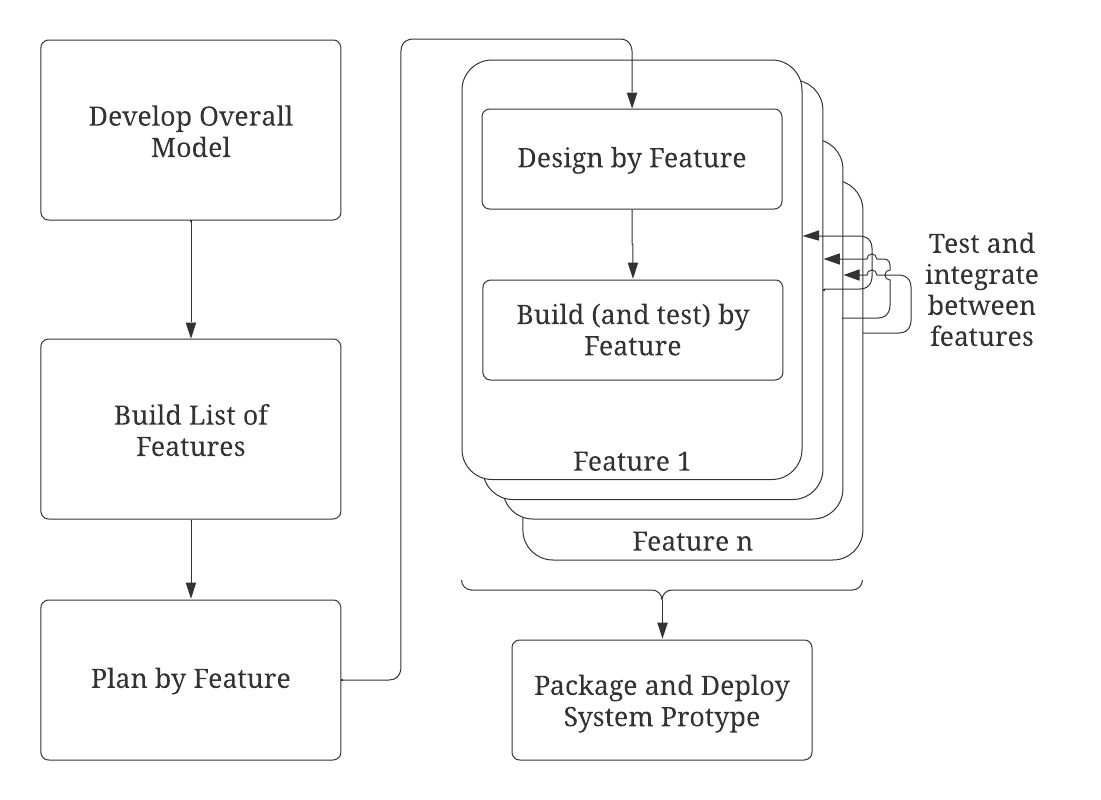
\includegraphics[width=\textwidth]{figures/Chapter3/Chapt3_DevFramework.jpeg}
    \caption{Modified Feature-Driven Development (FDD) Framework}
    \label{fig:FDDFramework}
\end{figure}

\subsection{Design, Building, Testing and Integration}

\textbf{Overall Model}

A high-level overall model or framework of what the application suite should be able to do based on general use-cases was first developed during the study’s proposal stage. It was there where the list of general features, to meet the general user requirements, were made. After which, the order of which each feature was to be designed, developed, tested, and integrated. This step ensured that each feature developed had their prerequisites met, facilitating the ease in integrating each of the application suite’s features into an overall cohesive system.

\textbf{Design and Development}

From the identified features, a rough design of how each feature would look like and how they integrate with each other was made. After which, following the FDD approach, each feature was designed and consequently developed, with the frontend (UI/UX) and backend (functions, data handling) codes of each feature being developed simultaneously.

\textbf{Testing and Integration}

\textbf{Alpha Testing and Feature Integration.} During and after the development of each feature, the feature is user-tested in order to ensure that the features work as intended and any bugs are immediately fixed. For features that rely on previous features to work (i.e. user account creation must work before user login), extensive user testing was done to confirm that the integration between each feature worked as intended. 

\textbf{User Tests.} Due to both time and technical constraints, testing was done solely by user testing rather than written and automated tests. Once the current feature and its prerequisite features have been tested, the development of the next feature would commence.

\textbf{Beta Testing.} Beta testing was conducted solely on the main user application by developers’ colleagues and relatives of varied ages (18, 24, 25, 30, 50, 54) to identify any remaining changes needed. Beta-testing of the PNP admin application was not possible due to time constraints, as it required to have a PNP staff (of different stations/precincts) assigned for receiving missing persons cases perform the tests. However, extensive alpha testing by developers was done to ensure that the PNP admin application was functional and intuitive.

\textbf{Implementation}

The final prototype is the fully functional application suite (including all the user interfaces) that meets the users’ requirements and passes all the tests during development.

\textbf{System Prototype}

The final product of the study, the HanApp main user app and the PNP app, is made available to the intended users. In this phase, routine maintenance and regular performance monitoring, particularly in the backend (traffic, database health, storage usage, API usage), is required to keep the application running smoothly. Post-release support would also include bug reporting and fixes, as well as backend and frontend optimizations to enhance the application’s efficiency and availability.

\section{Development Tools}
\subsection{Software}

\subsubsection{Github}
GitHub is a web-based tool that utilizes Git, an open source version control that enables several users to make distinct modifications to applications or software simultaneously \cite{digitalGovGitHub}. GitHub is currently being used by over 94 million software developers, 4 million plus organizations, and has created over 330 million repositories for varied software \cite{github}. 

Github was utilized in the project for storing the source code of the application suite and for the source version control during development, as well as for the repository for the LaTeX files for the study itself.

\subsubsection{Visual Studio Code}
Visual Studio Code (VS Code) is a compact yet capable source code editor for macOS, Windows, and Linux that runs on your desktop. It supports multiple programming and scripting languages like JavaScript, TypeScript, and Node.js, as well as a robust ecosystem of extensions for additional languages and runtimes (including C++, C\#, Java, Python, PHP, Go, and.NET) \cite{microsoft_2021}.

Visual Studio Code and Android Studio were used simultaneously as the primary source code editor, with Android Studio's Android Emulator being used to run the debug builds of the application suite.  

\subsubsection{Android Studio}
Android Studio is the official Integrated Development Environment (IDE) for developing Android mobile apps. It is based on the IntelliJ IDEA development tools and code editor. When compared to other IDEs, Android Studio is considered hefty; however, this is expected considering that it incorporates various integrations and add-ons like a flexible Gradle-based build system, built-in emulators, code templates, extensive testing tools, and many others to guarantee that development is as interactive and fluid as possible \cite{androidStudio}.

Android Studio comes with an Android Emulator which was the primary tool used for running and testing the application interfaces, as well as in debugging.

\subsubsection{Flutter}
Flutter is a Google open-source framework used for creating attractive, locally built, multi-platform apps out of a single codebase. For rapid efficiency and performance on any device, Flutter code compiles to ARM or Intel machine code, as well as JavaScript. Dart, a programming language designed for speedy programs on any platform, powers it \cite{flutter}. As the developers have aimed to deploy the proposed application on both the mobile (Android) platform for the main users, and on the Web (desktop)  platform for the side of PNP, Flutter is an outstanding choice out of all the available frameworks and languages.

Flutter (and the Dart programming language) was utilized in the development of HanApp's interfaces. Flutter packages were also imported for ease of development.

\subsubsection{Google Firebase}
As Firebase has a variety of products and services that it provides, such as Firebase Auth, which is a service that can authenticate users using only client-side code, Real-time Database, a NoSQL database service, and Firebase Storage, which is a file transfer service \cite{khawas2018application}, Firebase remains to be the most optimal choice for a serverless mobile application that may require the said services, such as with the proposed application.

Google Firebase is the sole and primary backend of the application suite. User authentication, database and data storage, and usage monitoring were all done under Firebase. Since Firebase is a serverless framework, utilizing Firebase as the application suite's backend allowed for development and testing without the use of a dedicated server infrastructure. 

\subsubsection{Google Maps}
Google Maps, one of the world’s most influential applications \cite{mehta2019google}, provides multiple location services needed in the application. This includes choosing the last seen location of the missing person being reported, or by integrating the maps view onto the application menu, where, users can see the location of the verified missing persons reports. 

\subsection{Hardware}
\subsubsection{Android Phone}
An Android phone is a type of smartphone that is operating using the operating system developed by Google, Android. Apart from the Android Studio's Android Emulator,  physical Android phones were utilized to test the debug and release builds of the application suite's main user mobile interface.

\subsubsection{Laptop}
The application was developed on laptop computers with the minimum specifications of an 8th generation Intel Core i3 CPU, and 8GB of RAM.

\subsection{Packages and Application Programming Interfaces (APIs)}

\subsubsection{Packages}
Software packages are a group of software programs that can be downloaded as a bundle of related products and used in the development of software.  They provide functionalities that are editable or customizable, in order to adjust to the specific requirements of organizations or developers that uses them \cite{jadhav2009evaluating}.

Packages in Flutter can be reviewed and downloaded from pub.dev, the official package archive for Flutter and Dart applications, which is also supported by Google \cite{pubdev}. Throughout the development of the applications, multiple verified packages from pub.dev have been used and are now essential to the functionality of the applications.

\paragraph{Firebase Packages.} Multiple Firebase packages from pub.dev have been utilized in the development of the application to better integrate the serverless backend service (Firebase) onto the applications' interface and services. These packages are firebase\_core, the overall prerequisite and helper package for all Firebase services in the Flutter application \cite{firebaseCore}, firebase\_auth, the package utilized in order to facilitate the registration, verification, log-in, and authentication persistence of users of the applications \cite{firebaseAuth}, and firebase\_storage and firebase\_database for the cloud storage needed by the images utilized by the applications, and the real-time database (RTDB) used to save multiple data needed by the applications \cite{firebaseAuth, firebaseStorage}.

\paragraph{Location Packages.} Packages were also needed in order to better facilitate and integrate maps and location services on the applications. These packages are google\_maps\_flutter, google\_maps\_flutter\_web, and location. The aforementioned google maps packages are used on the mobile application and the web applications respectively, for they are needed in order to display and better blend the user experience for using google maps services on the applications' targeted platforms. Location package, on the other hand, was used in order to ask for user permission before the application requests their current device's location.

\paragraph{Data Persistence Package.} Data persistence between views and states of the application is crucial in order to properly pass on volatile data from one page or interface, onto another within the application. For this purpose, the package shared\_preferences was used. This package allowed the developers to save data within the application itself or from the databases into a key-value pair in the platform-specific persistent storage for simple data like Strings and Boolean values, among other types \cite{sharedPreferences}.

\subsubsection{Application Programming Interfaces (APIs)}

\paragraph{Geocoding API.} The Geocoding API converts addresses directly into geographic coordinates, which may then be used to set markers on a map or position the map  \cite{geocoding}.

\paragraph{Maps SDK for Android API.} Maps SDK for Android is an API from the Google Cloud suite that adds maps functionality to Android apps and even on some embedded systems like Wear OS. This API enables Android-based hardware to use Google maps data, maps display, and maps gestures and responses. Additionally, it also provides some needed customizability on the maps interface by drawing polygons, lines, shortest paths, and customizable markers \cite{androidSDK}. 

\paragraph{Maps JavaScript API.} Maps JavaScript API is another API from the Google Cloud suite that enables maps functionality, customizability, and imagery for display on the web. The API features four map types, namely; roadmap, hybrid, terrain, and satellite \cite{javascriptSDK}.

\section{Application Requirements}

The following sections enumerate and discuss the backend, privacy and security, user interface, functional, and UI/UX design requirements that the the application suite needs to satisfy. For the purposes of tracking and verifying each feature during development and testing, a checklist of all features was developed. Table \ref{table:reqChecklist} lists down all the requirements and whether these requirements have been developed and achieved. 

% start of table
\begin{table}[!ht]
\caption{Checklist of Requirements}
\label{table:reqChecklist}
%table contents
\begin{tabular}{|ll|}
\hline
\multicolumn{1}{|c|}{\textbf{REQUIREMENTS}}                                                                                                                         & \multicolumn{1}{c|}{\textbf{\begin{tabular}[c]{@{}c@{}}ACCOMPLISHED\\ (Y/N)\end{tabular}}} \\ \hline
\multicolumn{2}{|l|}{\textbf{Backend Requirements}}                                                                                                                                                                                                              \\ \hline
\multicolumn{1}{|l|}{Serverless Architecture}                                                                                                                       &                                                                                     \\ \hline
\multicolumn{1}{|l|}{\begin{tabular}[c]{@{}l@{}}Realtime Database structure \\ for Main User and PNP profiles\end{tabular}}                                         &                                                                 {\hspace{1.75cm}}                           \\ \hline
\multicolumn{1}{|l|}{Realtime Database structure for Reports}                                                                                                       &                                                                                          \\ \hline
\multicolumn{1}{|l|}{Images and other media storage}                                                                                                                &                                                           {\hspace{1.75cm}}                                 \\ \hline
\multicolumn{2}{|l|}{\textbf{Privacy Requirements}}                                                                                                                                                                          \\ \hline
\multicolumn{1}{|l|}{User Password Encryption}                                                                                                                      &                                                                 {\hspace{1.75cm}}                           \\ \hline
\multicolumn{1}{|l|}{Data Privacy, Collection, and Usage}                                                                                                           &                                                          {\hspace{1.75cm}}                                  \\ \hline
\multicolumn{2}{|l|}{\textbf{User Interface Requirements}}                                                                                                                                                                                                       \\ \hline
\multicolumn{1}{|l|}{User (or Main) Interface}                                                                                                                      &                                                             {\hspace{1.75cm}}                               \\ \hline
\multicolumn{1}{|l|}{PNP Admin App Interface}                                                                                                                       &                                                             {\hspace{1.75cm}}                               \\ \hline
\multicolumn{2}{|l|}{\textbf{Functional Requirements}}                                                                                                                                                                                                           \\ \hline
\multicolumn{1}{|l|}{User Registration}                                                                                                                             &                                                               {\hspace{1.75cm}}                             \\ \hline
\multicolumn{1}{|l|}{PNP Admin Account Creation}                                                                                                                    &                                                               {\hspace{1.75cm}}                             \\ \hline
\multicolumn{1}{|l|}{Reporting and Receiving Updates}                                                                                                               &                                                                    {\hspace{1.75cm}}                        \\ \hline
\multicolumn{1}{|l|}{Save Report as Draft}                                                                                                               &                                                                    {\hspace{1.75cm}}                        \\ \hline
\multicolumn{1}{|l|}{Receive, Manage, and Verify Reports (PNP)}                                                                                                     &                                                            {\hspace{1.75cm}}                                \\ \hline
\multicolumn{1}{|l|}{\begin{tabular}[c]{@{}l@{}}Accessing PNP-Verified Reports and receiving \\ Location-based notification for PNP-verified MP cases\end{tabular}} &                                                {\hspace{1.75cm}}                                            \\ \hline
\multicolumn{2}{|l|}{\textbf{UI/UX Design Requirements}}                                                                                                                                                                                                         \\ \hline
\multicolumn{1}{|l|}{Application Icon Design}                                                                                                                       &                                                              {\hspace{1.75cm}}                              \\ \hline
\multicolumn{1}{|l|}{User Interface Design}                                                                                                                         &                                                              {\hspace{1.75cm}}                              \\ \hline
\multicolumn{1}{|l|}{User Experience Design}                                                                                                                        &                                                              {\hspace{1.75cm}}                              \\ \hline
\end{tabular}
\end{table}
% end of table

\subsection{Backend Requirements}

Listed below is the overall structure of all connections and relationships among all data, interfaces, users, and the serverless service. 

\subsubsection{Serverless Architecture}
The overall serverless architecture of the application suite and its system is portrayed in figure \ref{fig:ServerlessFirebase}. Firebase, as the serverless service being utilized, serves as the storage medium for all data being utilized in all of HanApp’s interfaces. 

\begin{figure}[!h]
    \centering
    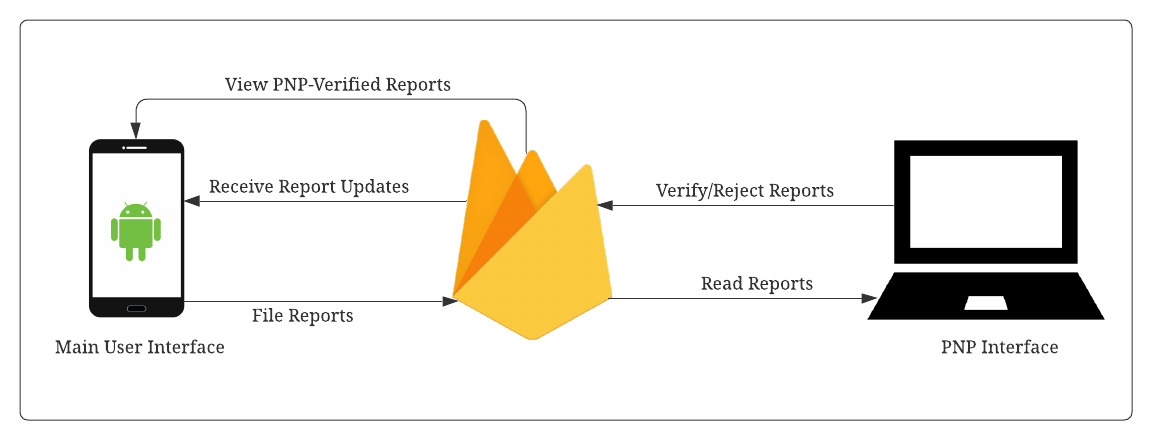
\includegraphics[width=\textwidth]{figures/Chapter3/Chapt3_ServerlessArchitecture.jpeg}
    \caption{Client-Serverless Architecture with Firebase}
    \label{fig:ServerlessFirebase}
\end{figure}

\subsubsection{Database Structure Design}
Creating a comprehensive map of the data to be used in the application suite (and how they interact with each other) was a crucial requirement prior to developing HanApp's database in Firebase's Realtime Database (RTDB). This would ensure the completeness and cohesiveness of the data, as well as minimize redundancy and confusion when developing the database. In order to achieve this, an Enhanced Entity-Relationship Diagram (ERD), shown in Figure \ref{fig:EERD}, was designed which provides an overview of the HanApp application suite's entities and their relations.

\begin{figure}[!h]
    \centering
    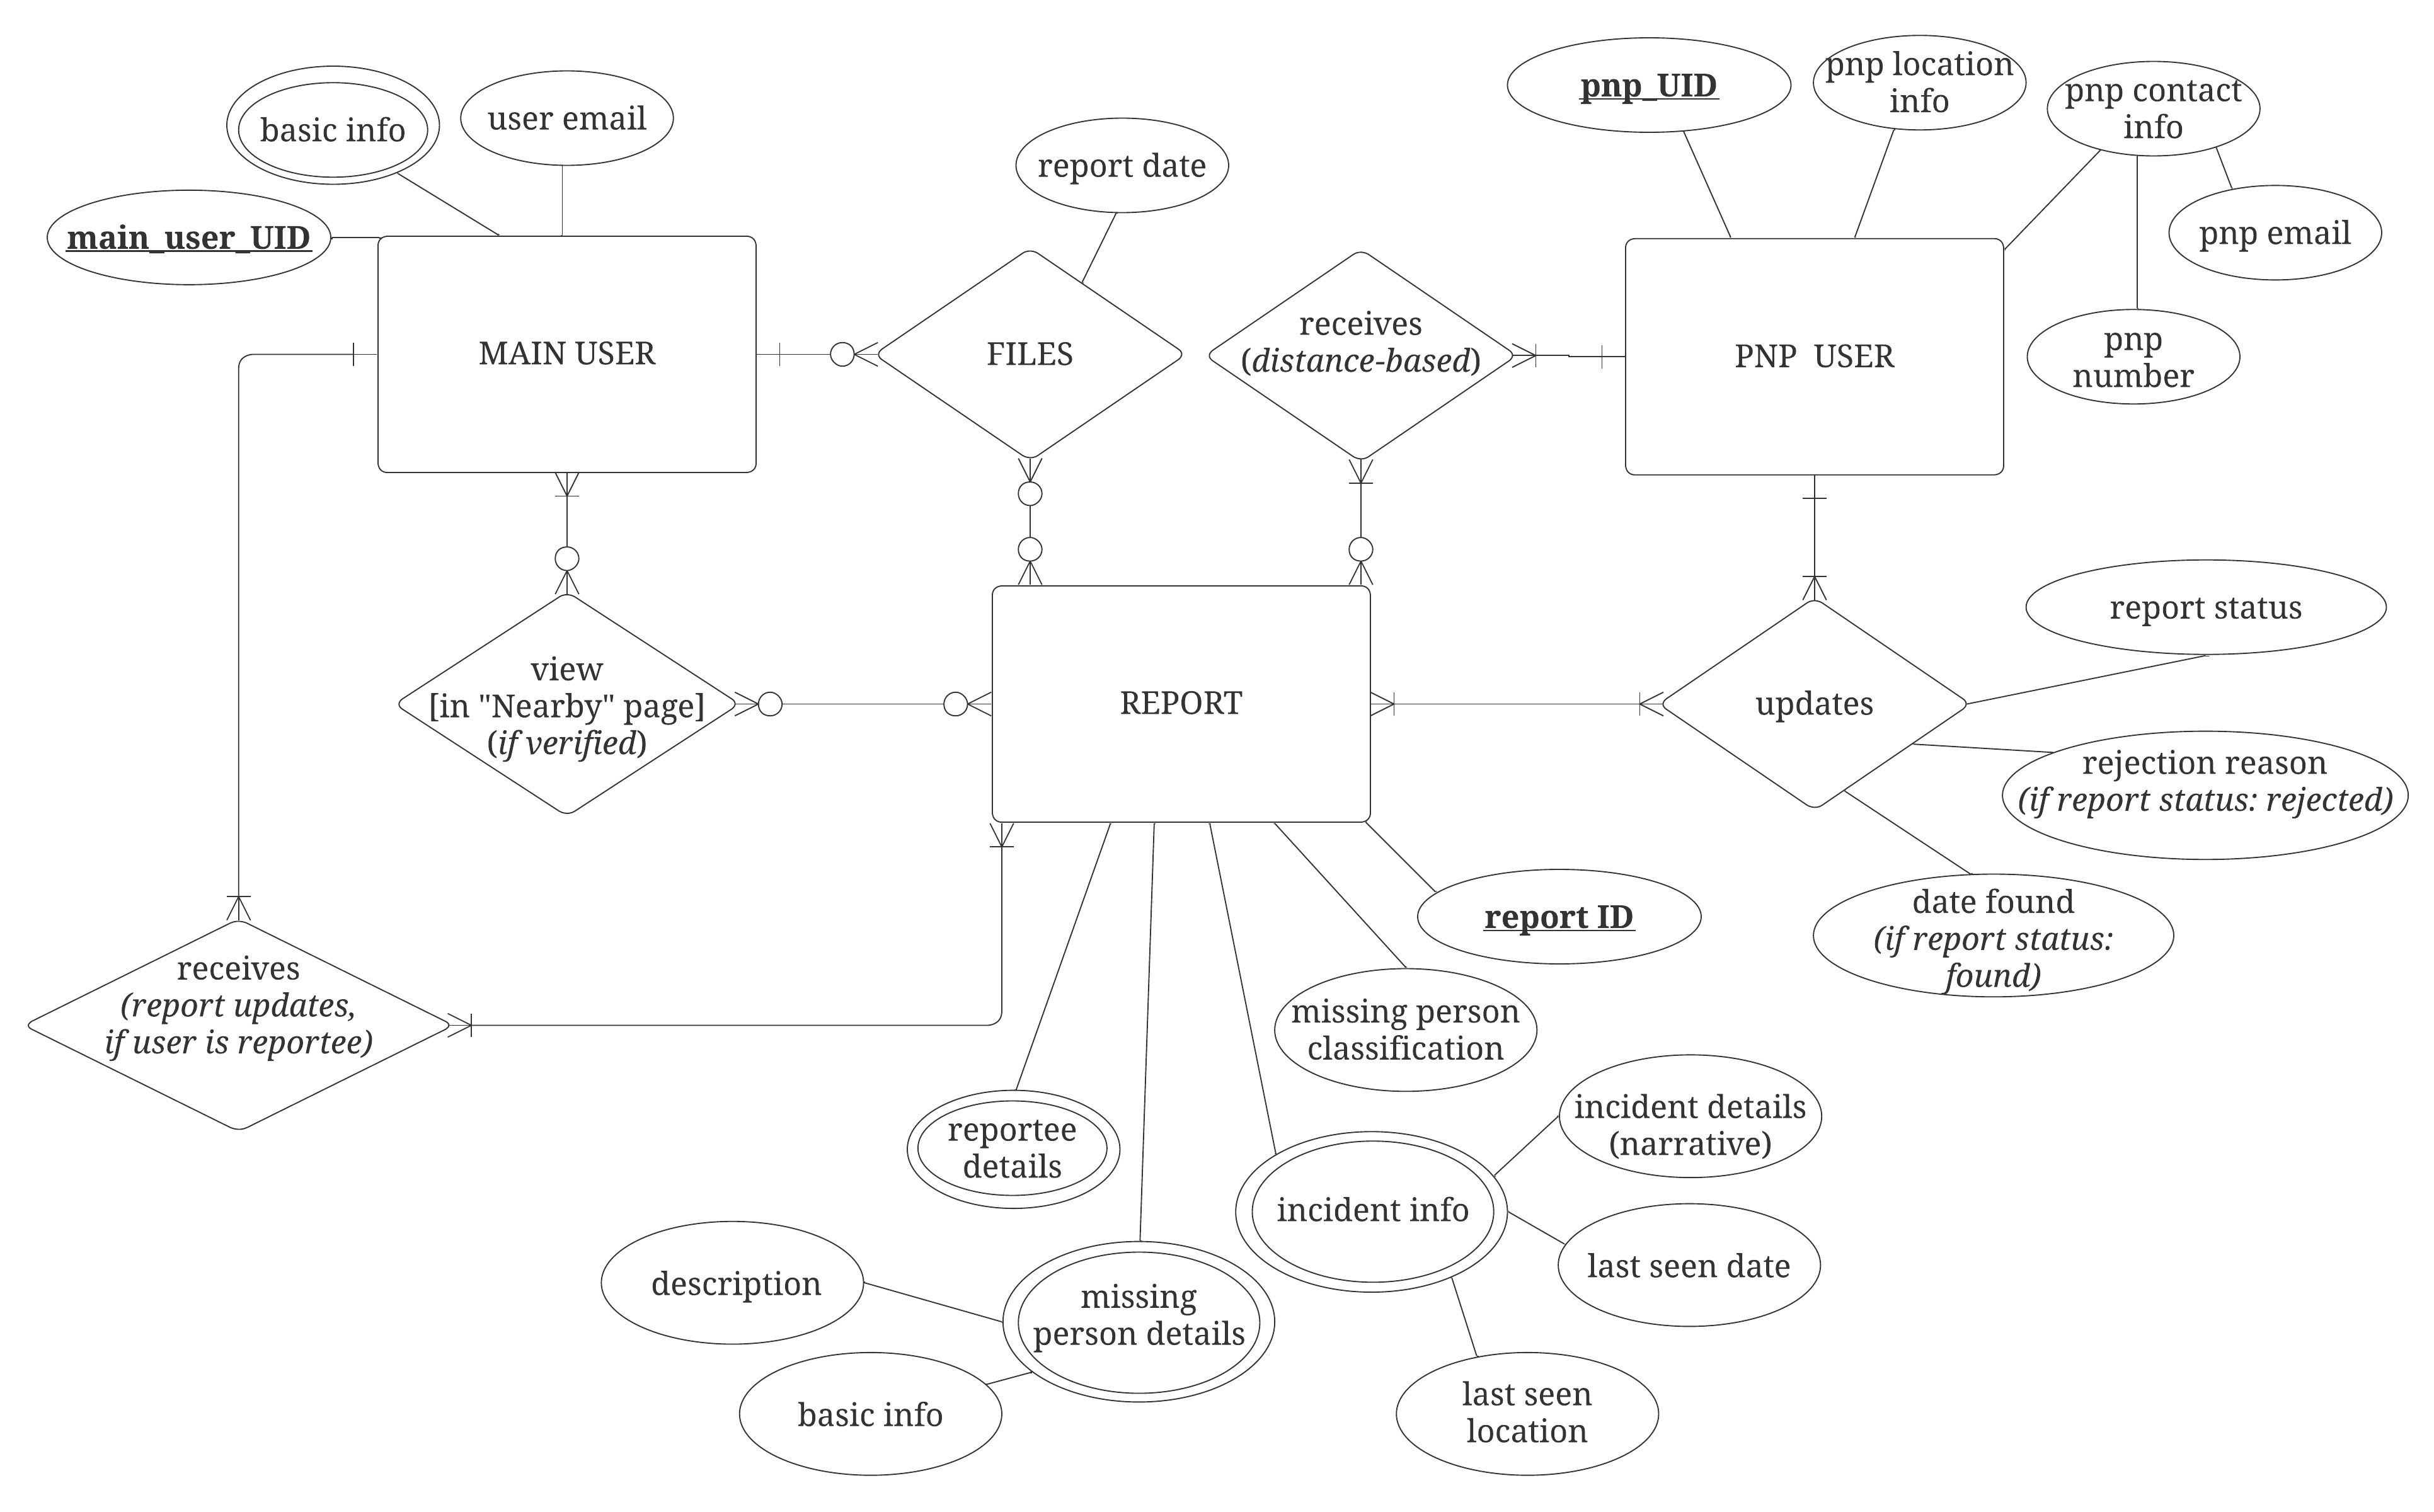
\includegraphics[width=\textwidth]{figures/Chapter3/eerd.jpeg}
    \caption{Enhanced Entity-Relationship Diagram for HanApp Database Structure}
    \label{fig:EERD}
\end{figure}

For a more compact and comprehensive visualization of the HanApp application suite’s database entities, relationships, and read/write rules, an Entity-Relationship(ER) - Database Schema hybrid diagram, as shown in Figure \ref{fig:hybridERDSchema}, was designed. The succeeding backend requirements were based on the aforementioned hybrid diagram.


\begin{figure}[ht!]
    \centering
    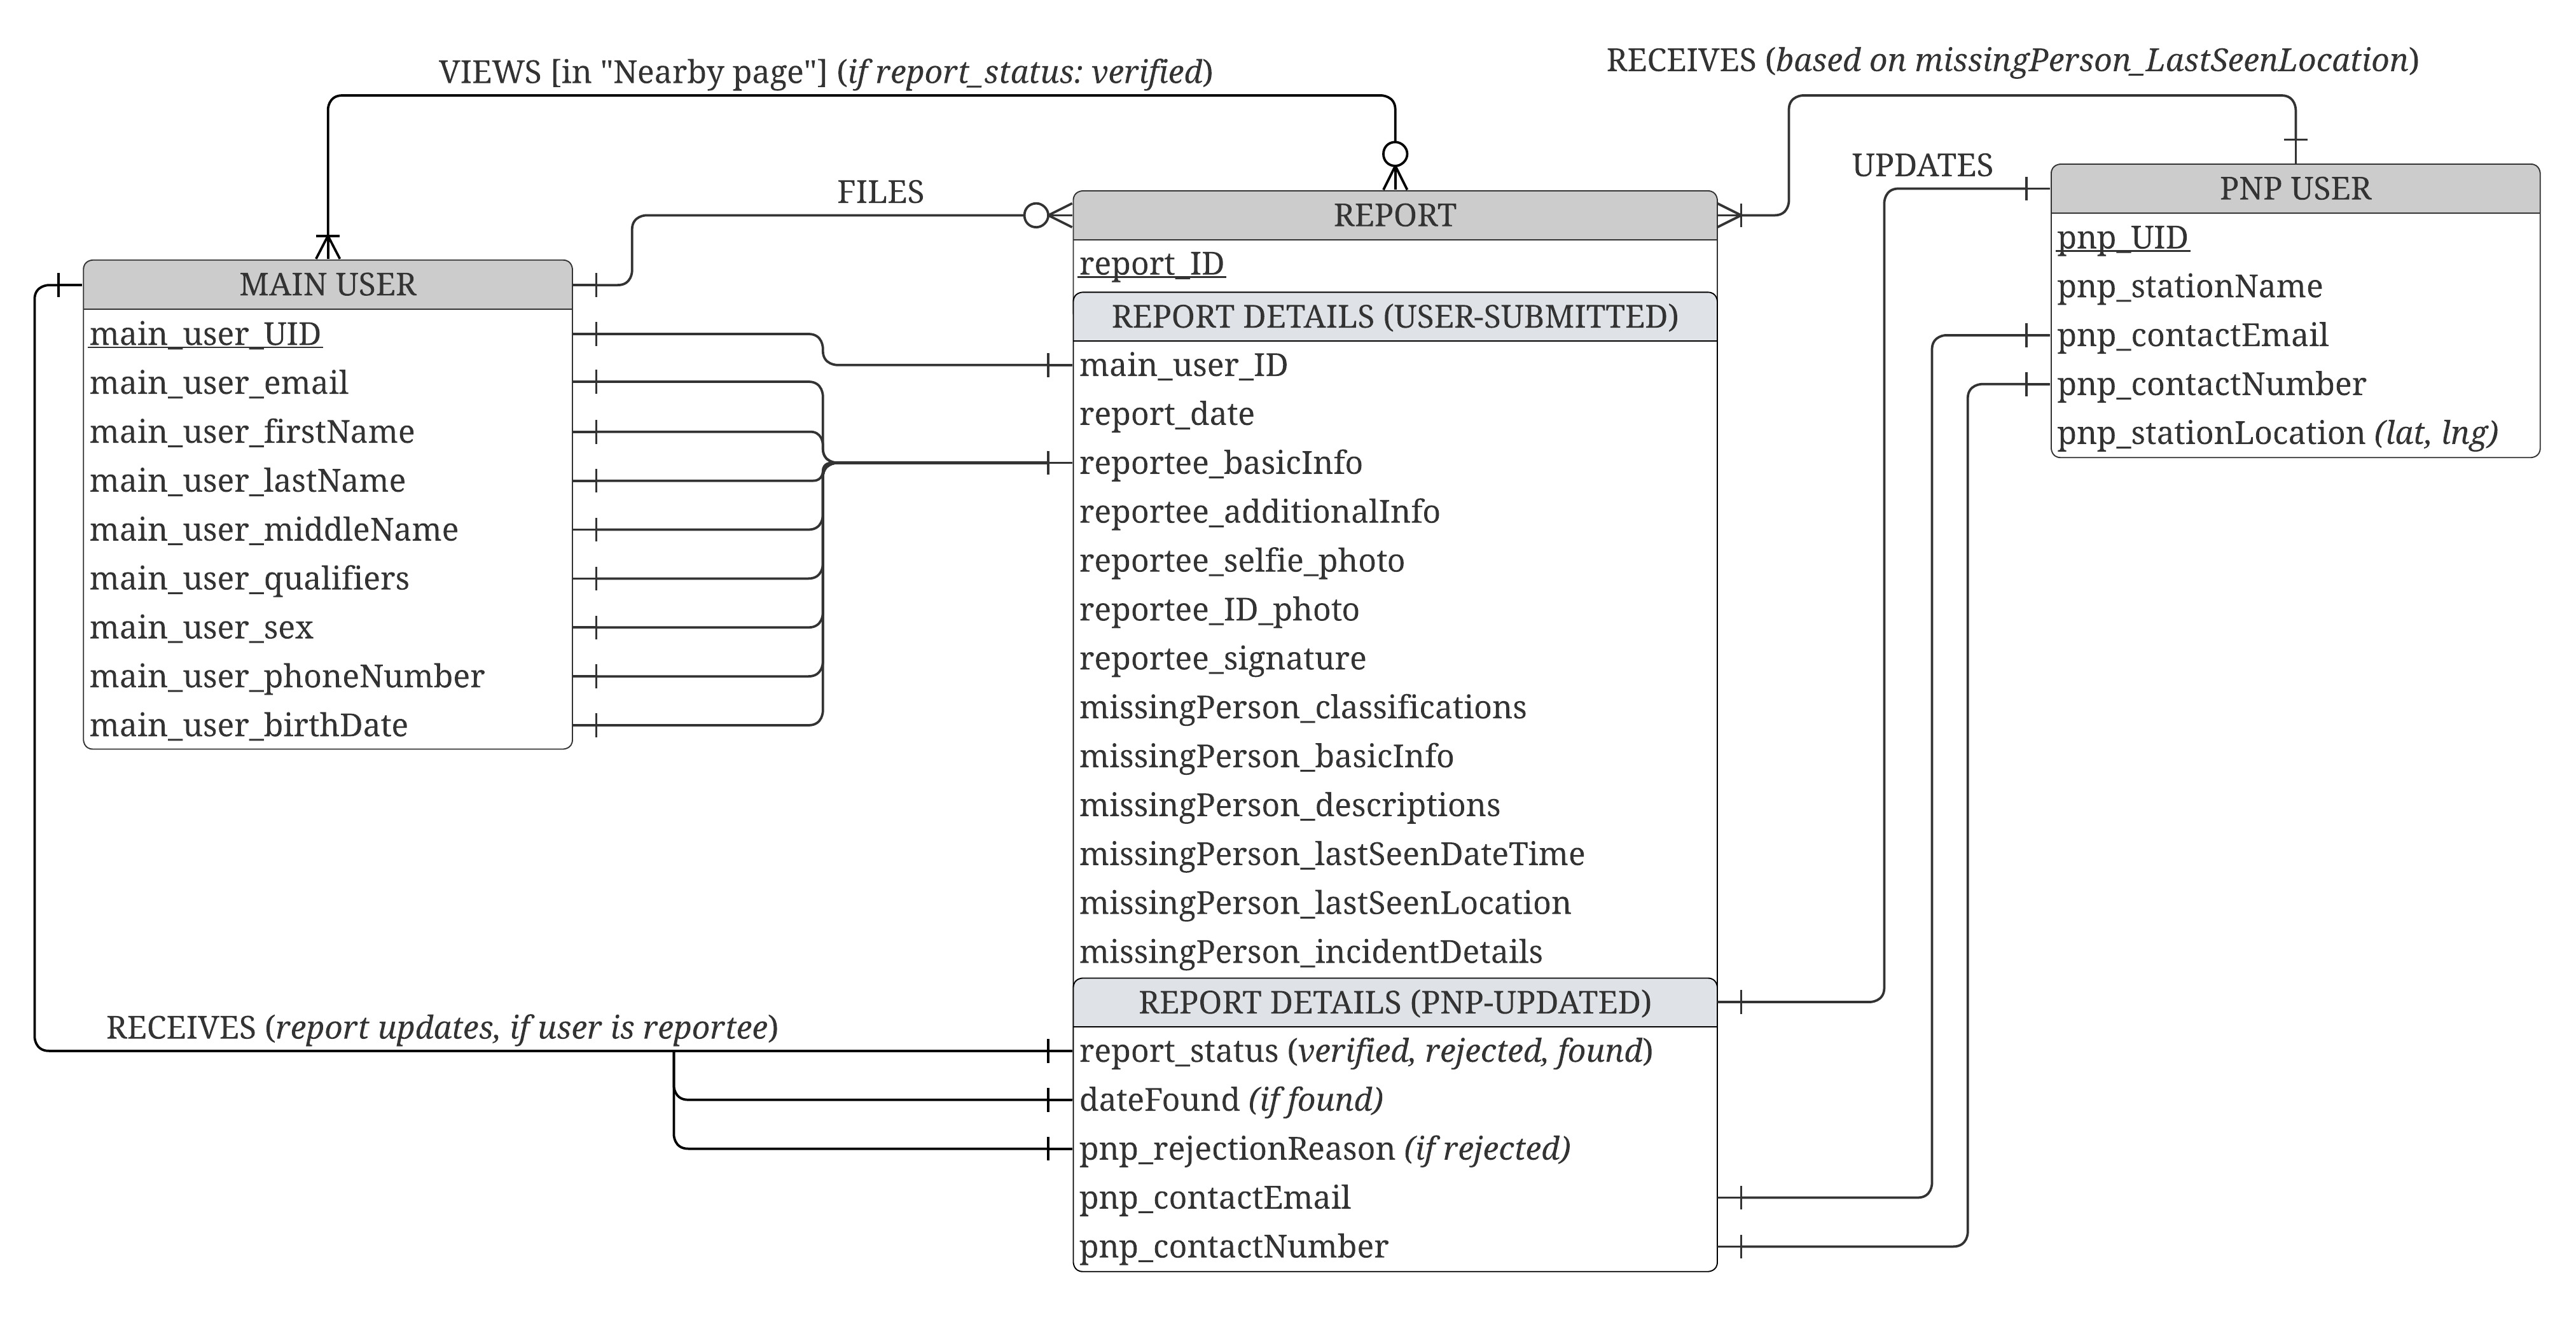
\includegraphics[width=\textwidth]{figures/Chapter3/erd_schema.jpeg}
    \caption{Entity-Relationship - Database Schema Hybrid Diagram for HanApp Database Structure}
    \label{fig:hybridERDSchema}
\end{figure}

\subsubsection{Realtime Database structure for Main User and PNP profiles}
Each profile type will be a node just under the root node as child nodes, namely, Main Users, and PNP Accounts. 

\subsubsection{Realtime Database structure for Reports}
As Firebase’s real-time database is structured as a tree, sent reports are listed as child nodes of the user who sent them, under a more general `Report' node. This way, it will make it easier to know who has filed what, and only the user who has filed an unverified report can directly see it. Once the PNP Admin interface has verified it, then that report will be displayed publicly.

\subsubsection{Images and other media storage}
The real-time database only functions on non-media data like text, integers, and location data; therefore, images used within the application interfaces (user image, missing person image) will be stored in Firebase’s cloud storage. 



\subsection{Privacy and Security Requirements}

Because the application deals with sensitive information, it is critical to consider security and data privacy concerns to ensure that their data is not illegally accessed or utilized beyond the purposes of the application.

\subsubsection{User Password Encryption}

Passwords for users (main and PNP admin users) should be encrypted so that neither the developers nor other users may access them. 

\subsubsection{Data Privacy, Collection, and Usage}

Users will also be required to agree to having their information used solely for the purposes of reporting and disseminating missing persons cases. In line with this, the user will be required to agree to having their data used and by the PNP in line with their guidelines and by the application for dissemination  once verified. Moreover, the users will be informed that their data is protected under the Data Privacy Act (RA 10173).

\textbf{Data collection scope}. The application will not collect information for any secondary purposes, and as such, no other information will be required from users apart from those used for logging into the account and reporting, disseminating, and viewing (verified) missing persons cases.

\textbf{Location Data Anonymity.} Lastly, user location data, which is utilized for location-based notification of verified missing persons cases, will not be collected by the application to protect users’ privacy.


\subsection{User Interface Requirements}

\subsubsection{User (or Main) Interface}

The User use-case diagram in Figure \ref{fig:UseCaseMain} illustrates all the possible tasks that a normal user could do within the main user application. User account creation will be done within the application itself, through Firebase Auth’s authentication service using a registered email address and password. After the user has registered and confirmed their email address, their account will be created. 

\begin{figure}[!h]
    \centering
    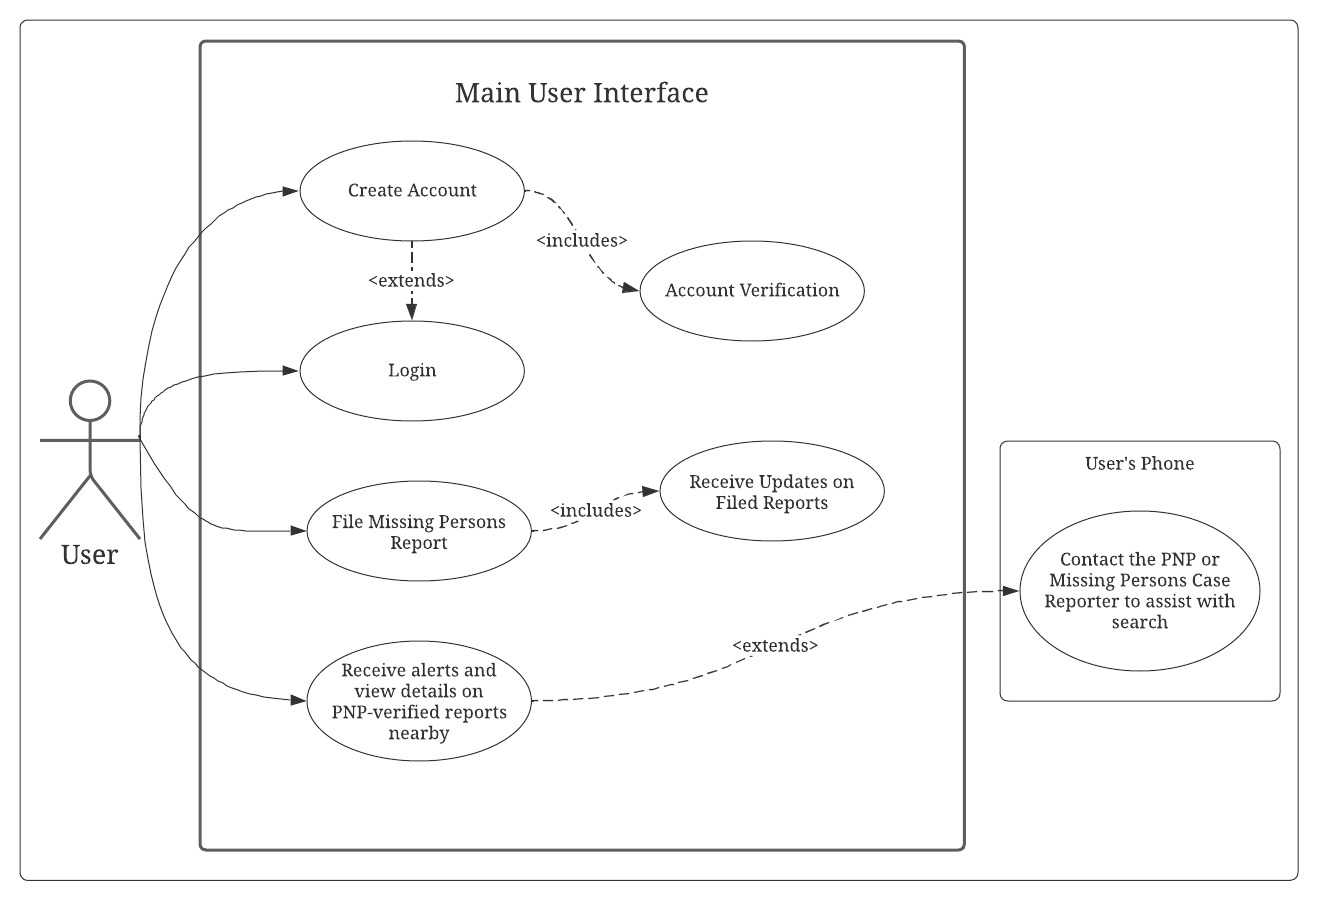
\includegraphics[width=\textwidth]{figures/Chapter3/Chapt3_UseCase_Main.jpeg}
    \caption{Use-Case Diagram for User (Main User Interface)}
    \label{fig:UseCaseMain}
\end{figure}

The main features of this application interface is with the reporting and viewing of missing persons cases. This is done through the application by filling out a form with the details required for the missing persons report, which would then be filed towards the most logically sound police-station. Users can also receive notifications and view information regarding  descriptions and features of any PNP-verified missing persons cases within their area.

\subsubsection{PNP Admin App Interface}

The PNP and PNP Admin interface use-case diagram is shown in Figure \ref{fig:UseCasePNP}. The PNP admin accounts are created in a different manner compared to the previously stated accounts. First, PNP admin accounts cannot be created through the PNP admin interface (e.g., a ``Register" option) in order to control and limit the number of admin users within a police station to only one, who can only handle missing persons reports within their vicinity. 

Local police stations can request PNP admin accounts from the developers in order for it to be recognized as a PNP account rather than any other user account. Once a PNP admin has logged in to the PNP admin interface, he or she, as an official, can then browse and either verify or reject missing person reports filed within their jurisdiction.
\begin{figure}[!h]
    \centering
    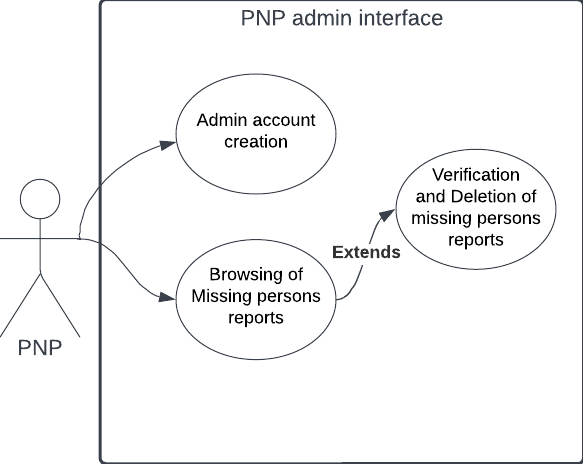
\includegraphics[scale=0.5]{figures/Chapter3/Chapt3_UseCase_PNP.png}
    \caption{Use-Case Diagram for PNP (PNP Admin Interface)}
    \label{fig:UseCasePNP}
\end{figure}


\subsection{Functional Requirements}

The following are the user requirements, for both the main users and PNP users, identified during the design phase of the application suite's development in order to meet the study's objectives. 

\subsubsection{User Registration}
Main application users should be able to launch their respective application interfaces and register through the log-in and registration page in-app. Once verified and registered, users can then utilize and log in into the application. 

\subsubsection{PNP Admin Account Creation}

For security reasons, creation of PNP Admin accounts will be highly regulated. As such, for the initial release build of the application suite, the PNP accounts are created upon the PNP's request to the developers to create their admin account.

As proof of concept and for testing purposes, the PNP Admin test accounts will be hard-coded by the developers to simulate the process of PNP requesting for an account. 


\subsubsection{Reporting and Receiving Updates}
General users should be able to fill out and send the MP case report form via the main app interface to the PNP station where the reported person went missing has the closest vicinity to, and receive updates via the main app with regards to the status of the report.

With regards to reporting, it is of utmost importance that the report form pages of the main user interface should be intuitive, and be able to condense and simplify the forms required in the PNP's guidelines on reporting missing persons cases.

As seen in Figure \ref{fig:seqDiaReport} sequence diagram, reporting and receiving updates is very straightforward: the user (reportee) needs to fill out the MP report form, it is then received by the PNP through their PNP Admin App interface, and if the person is indeed missing (and not yet reported, or registered as already found or dead in the PNP's own Missing and Found Person Database (MFPD)), then the PNP can verify the report. If any updates are made, such as if the MP is found, it will be reflected in the user’s app soon after.

\begin{figure}[ht!]
    \centering
    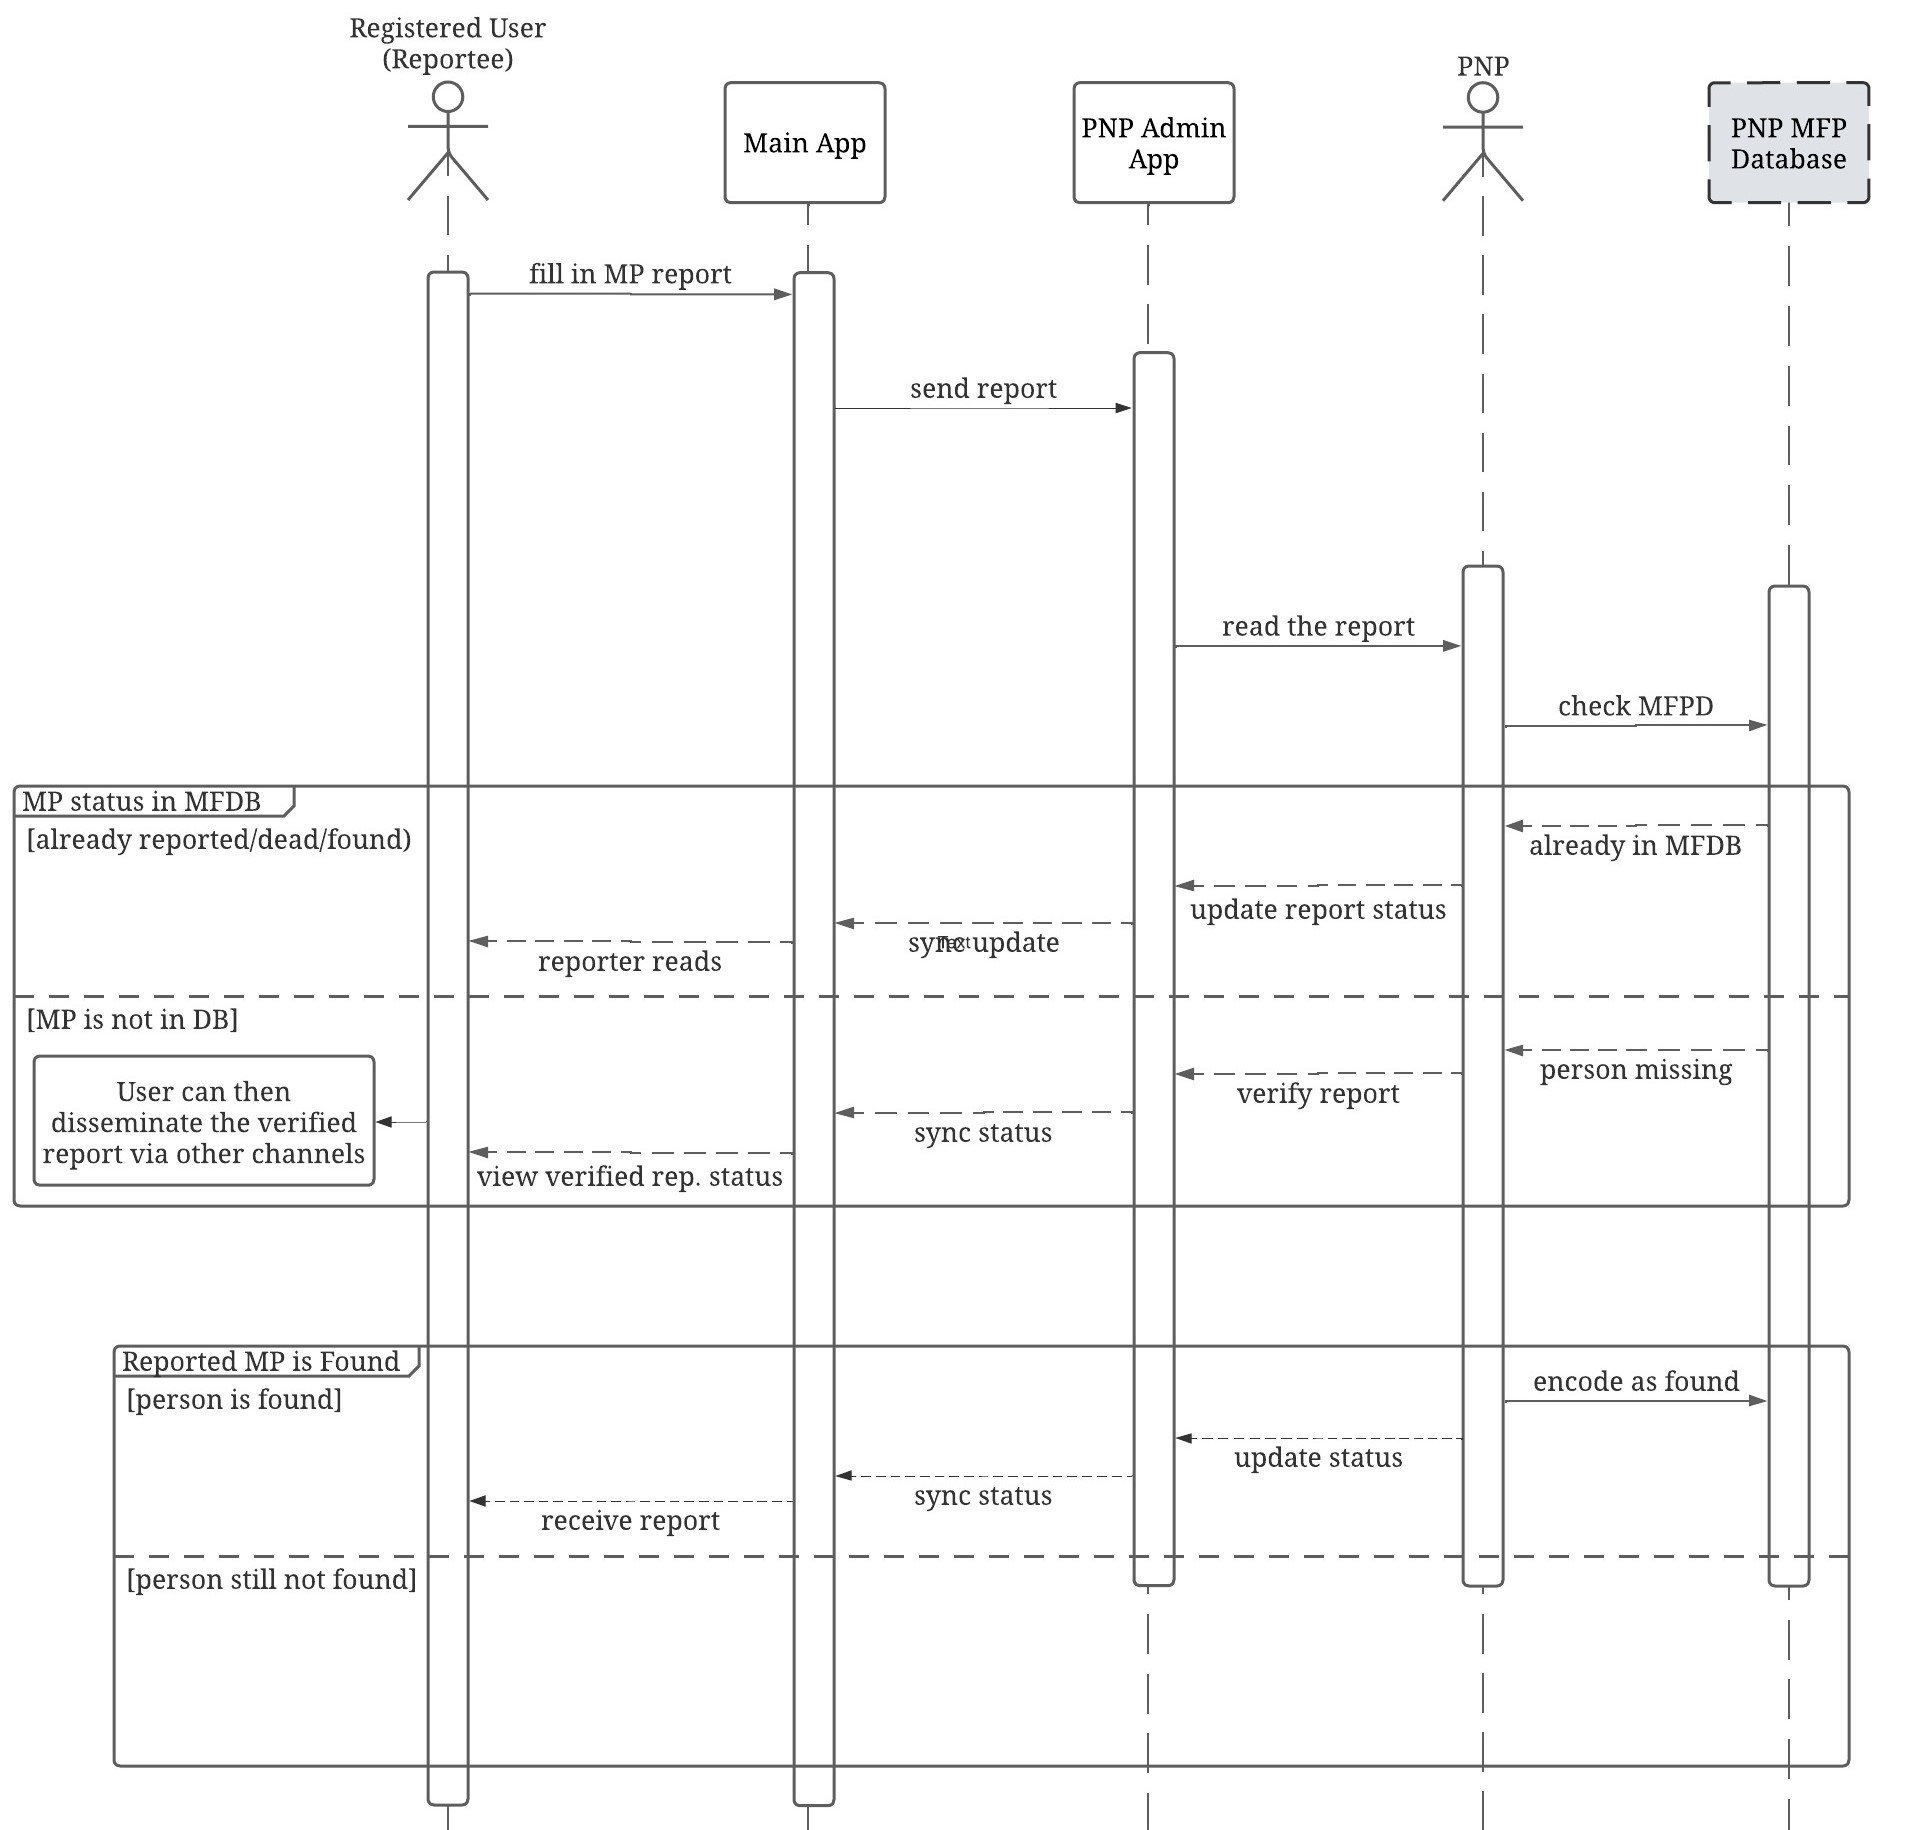
\includegraphics{figures/Chapter3/Chapt3_seqDiag_report.jpeg}
    \caption{Sequence Diagram for Reporting, Updating, and Verification of MP cases}
    \label{fig:seqDiaReport}
\end{figure}

It is also an important requirement that any reports made by users (reportee) are sent to the PNP Admin Account of the A/MP's last known location’s nearest PNP station, as mentioned prior. As seen in Figure \ref{fig:ERDReportee}, many users should be able to submit MP case reports of a specific location to the PNP through the application, but they will only be routed to the PNP Admin Account closest (and within the vicinity) of the missing person's last known location.
\begin{figure}[ht!]
    \centering
    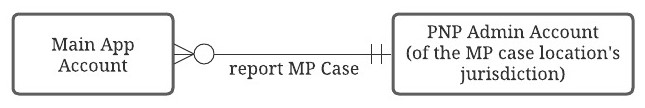
\includegraphics[width=\textwidth]{figures/Chapter3/Chapt3_ERDiag_reporteePNP.jpeg}
    \caption{Entity Relationship Diagram of Main App Account Reporting to PNP Admin Account}
    \label{fig:ERDReportee}
\end{figure}

\subsubsection{Save Report as Draft}
One of the main issues with in-person reporting  process is the number of fields and forms required to be filled-in completely in order for the PNP to proceed with processing the report. This issue is partially addressed  in the previous requirement, such that the researchers ensured that the forms are condensed and simplified. 

However, despite this, the report forms are still considerably lengthy, and it is possible that the reportee is unable to complete the form in one sitting. As such, it is crucial that the main user app's report forms feature a ``Save as Draft" feature that allows the user to either discard the report or save it as a draft which they can continue filling out at a later time.  

\subsubsection{Receive, Manage, and Verify Reports}

The PNP Admin should be able to receive reports from users through the PNP Admin app. PNP Admin should also be able to put updates on the report (i.e. MP case already reported, MP reported is already found, etc.), and also verify the report to state that the MP is categorized as missing. This can also be seen in the sequence diagram in Figure \ref{fig:seqDiaReport}. 

\subsubsection{Accessing PNP-Verified Reports and receiving Location-based notification for PNP-verified MP cases}

Users in a certain radius of the PNP-verified MP case  should receive notifications about an MP case in their area. Users can tap on the marker where the MP was last seen to view the concise details of the MP in the report. As seen in Figure \ref{fig:diagramLocation}, all users should be able to view all PNP-verified reports, including those outside their radius, but will only receive notifications for cases within the user's radius.

\begin{figure}[!h]
    \centering
    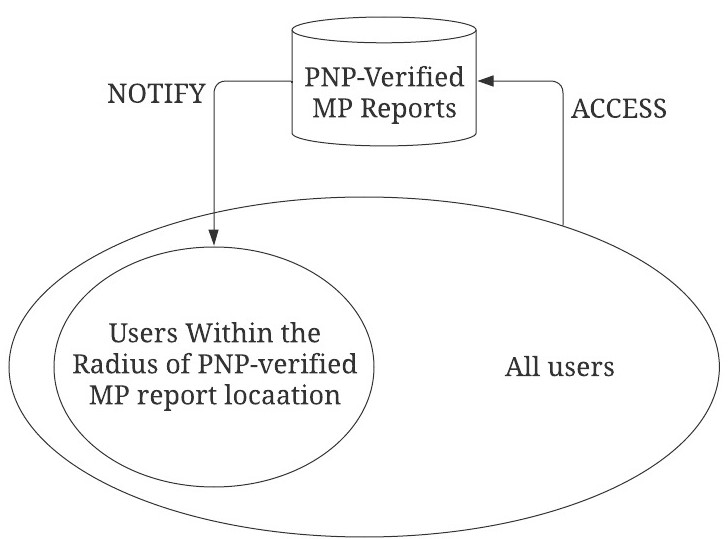
\includegraphics[scale = 1.50]{figures/Chapter3/Chapt3_Diag_locationBasedNotif.jpeg}
    \caption{Diagram for PNP-Verified Reports Access and Notification System}
    \label{fig:diagramLocation}
\end{figure}

\subsection{UI/UX Design Requirements}

As an application suite which is used in an emergency services and crisis context, HanApp's user interface and user experience (UI/UX) should have ease of use and accessibility as a priority. As such, listed below are the UI/UX  design requirements for the application suite.

\subsubsection{Application Icon Design}

HanApp's Icon design should be distinct, meaningful, and cohesive with the application suite's UI/UX design and color theme. It should give the users the impression that the application is about making reporting and dissemination of missing persons cases.

\subsubsection{User Interface Design}

\textbf{Colors.} The colors used in the application should prioritize accessibility and simplicity while still providing a cohesive and pleasing aesthetic. More importantly, colors should be of high contrast in order to make the application more accessible to those with color blindness.

\textbf{Text Font.} The chosen font family for the application suite should be legible and adequately-sized for readability. The text font choice should ensure that even those with mild visual impairment may still use the app.

\textbf{In-App Icons.} The icons to be used in the application should be obvious, commonly-used, and/or easy to understand.

\textbf{Layout and Spacing.} The layout of text form fields, buttons, and other visual elements should have appropriate sizes and spacing in order to minimize any user errors or confusion, and prevent the application pages from looking cramped.  

% \hfill\\
\textbf{User Experience Design}

\textbf{Application Language.} The language to be used in the application suite is English. Although the scope of operations for the application suite is the Philippines, English is the widely used language for education and business in the country and is a neutral language that allows the application to be accessible to most users. Moreover, the language used in the PNP's forms for filing and processing missing persons cases are also in English. More importantly, the language used in the application should be simple and straightforward in order to cater to more users regardless of educational background or cognitive abilities.

\textbf{Report Form Design and Validation.} 
The report forms are a major part of the application, and it is imperative that the forms are  straightforward and intuitive. As such, there should be thorough planning on the use of radio buttons, checkboxes, date pickers, text form fields, and other user input elements to ensure that filling of reports is not only easier but also minimizes user input error. Lastly, there should be validation checks to ensure that all information required by the PNP are provided completely and correctly by the reportee.               %LaTeX source file for Chapter 3: Methodology
%   Filename    : chapter_4.tex 
\chapter{Results and Discussions}
%\This chapter presents the results or the system of your SP. Include screenshots, tables, or graphs and provide the discussion of results.
This chapter presents the results of the study, specifically the HanApp application suite's various interfaces and screens, features, and backend framework implementation. As such, the figures shown herein are screenshots of HanApp's release build interfaces as well as the backend framework, particularly Firebase.

\section{PNP Admin Interface}
The PNP Admin interface focuses on the managing and administrative side of the applcation suite, providing the necessary access, features, and screens to manage all missing persons reports sent by users through HanApp's main user application interface.

\subsection{PNP Account Creation and Login Screen}

Figure \ref{fig:PNP1} Login page of the PNP-side app will authenticate the user to enforce access in the reports management system of the missing persons. Input fields are provided for username and password for PNP’s credentials. When the PNP Admin user is having troubles with regards to authentication or registration, they would need to contact the developers directly, either to get an admin account for their respective PNP outpost, or to reset the password of their corresponding admin accounts. 

\begin{figure}[!h]
    \centering
    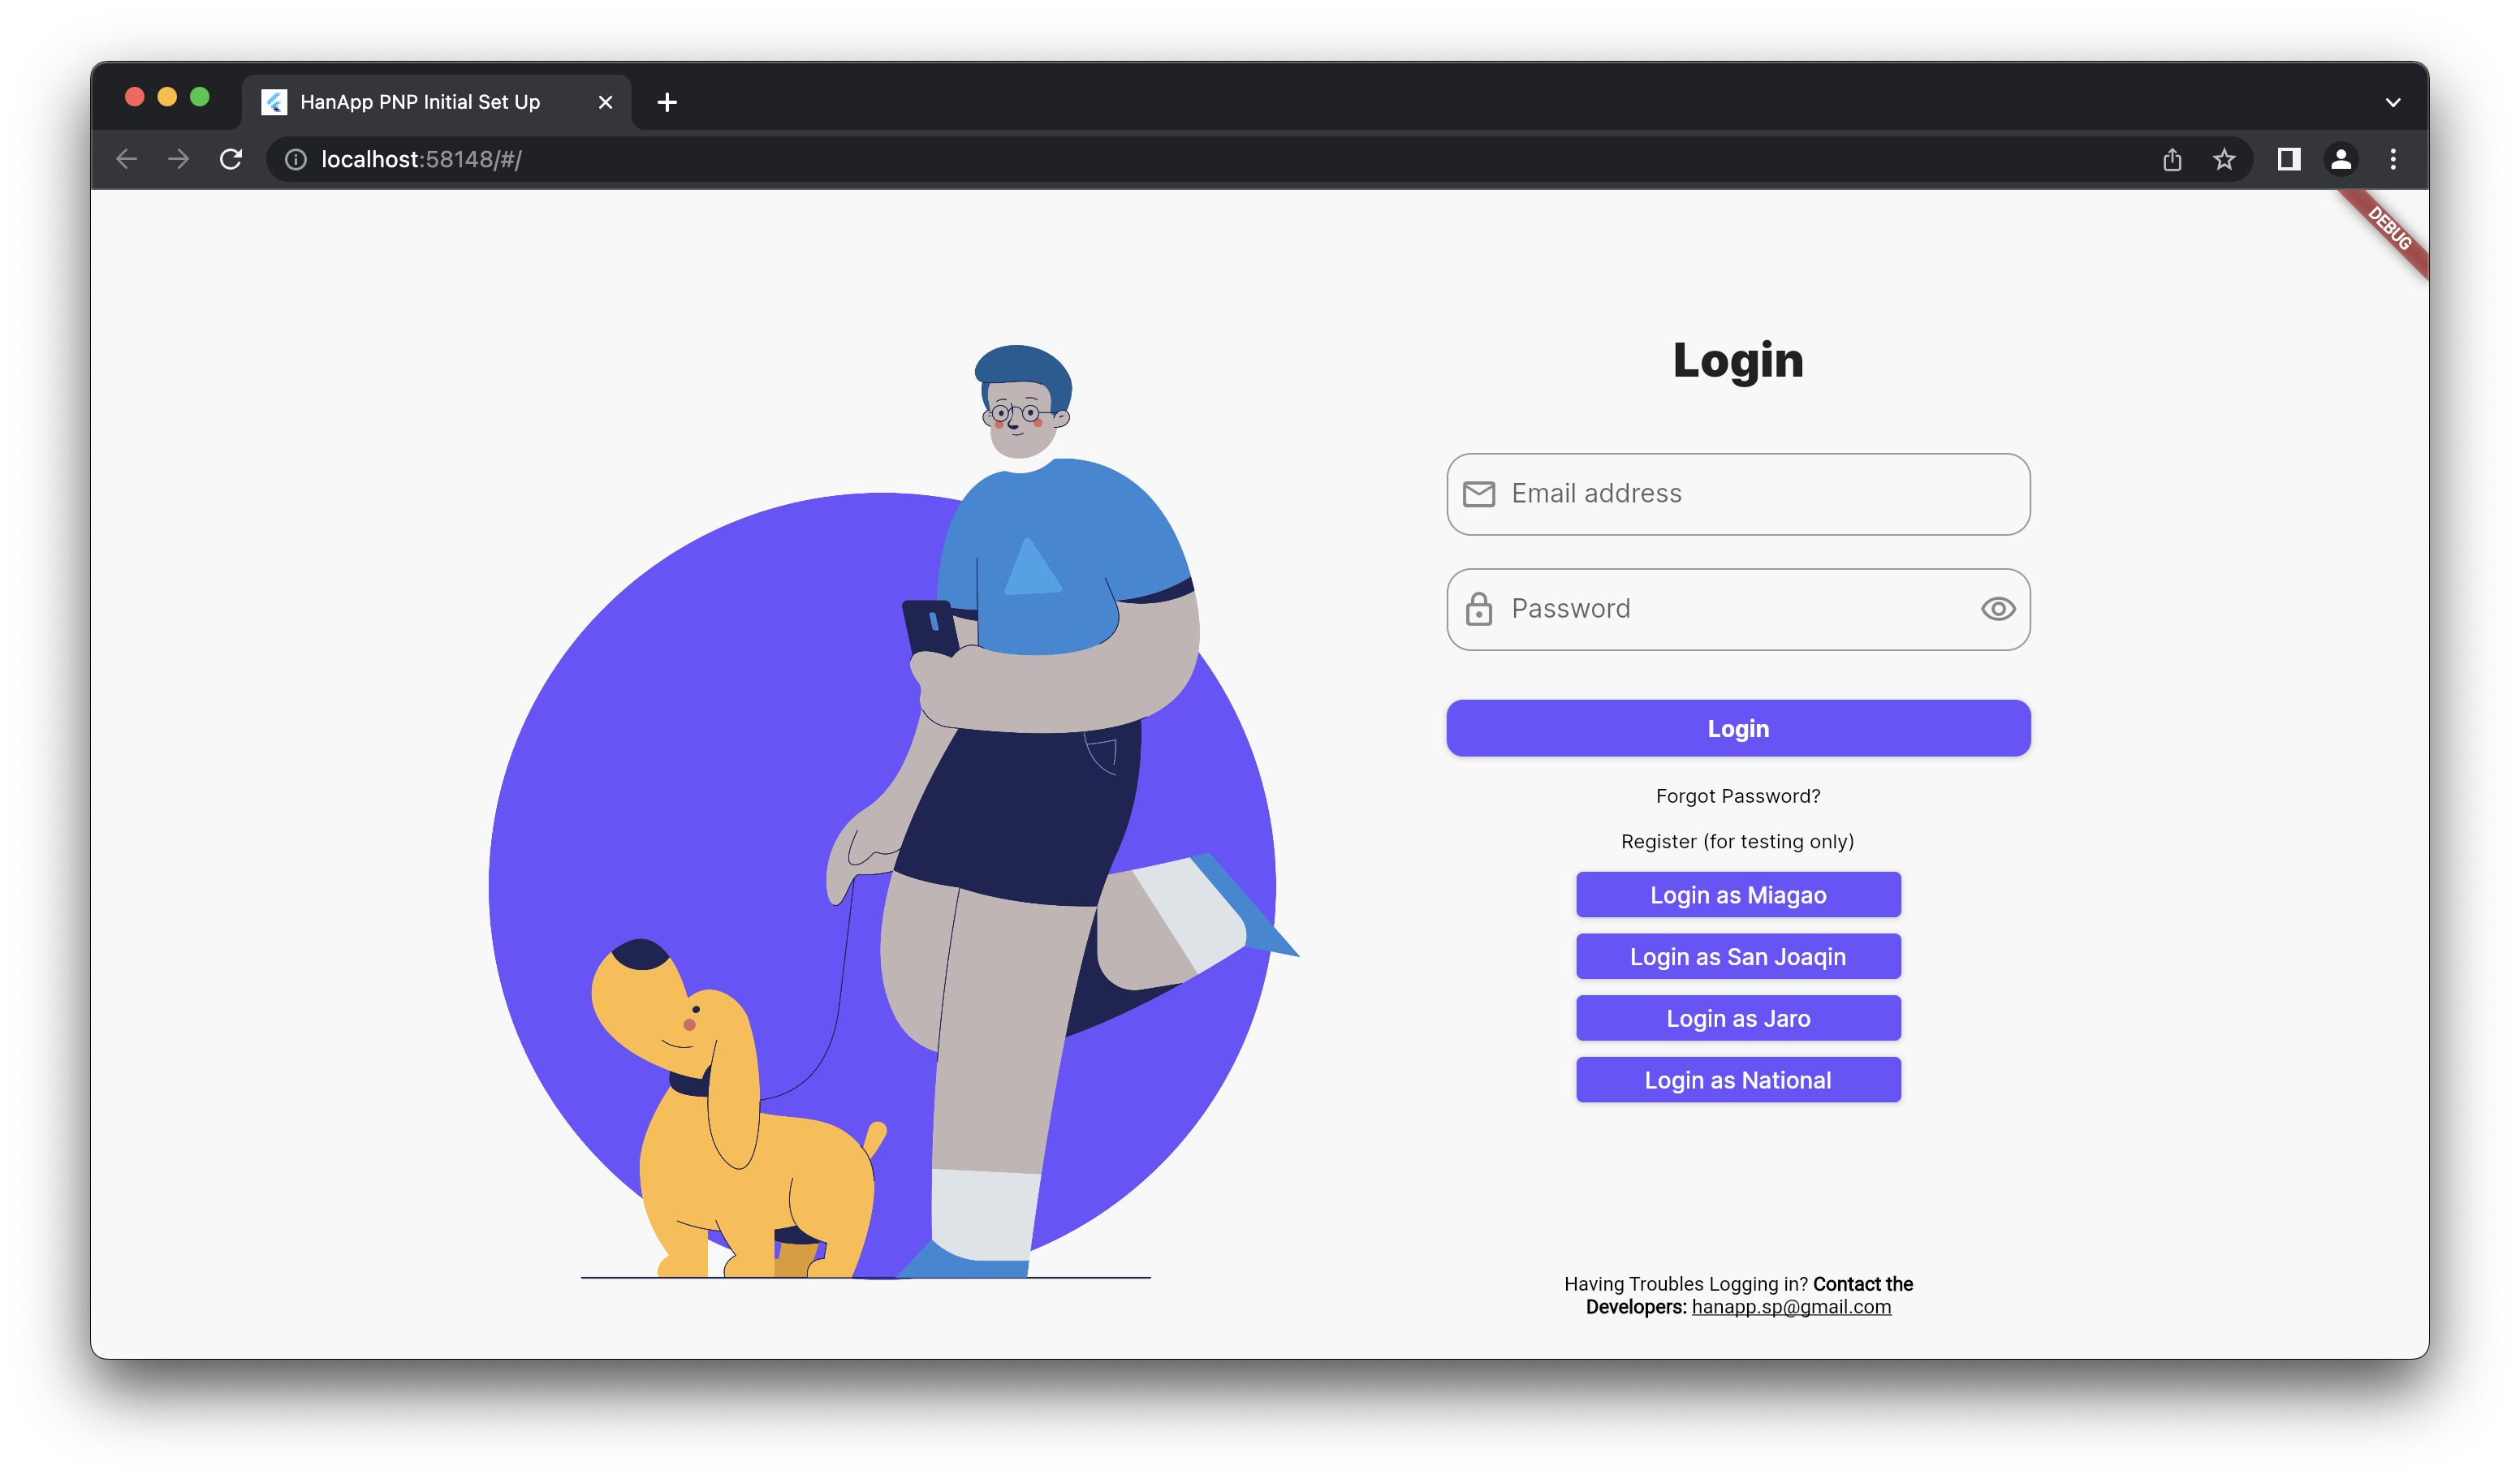
\includegraphics[scale=0.25]{figures/Chapter4/PNP/Login.png}
    \caption{PNP Admin Login Page}
    \label{fig:PNP1}
\end{figure}

\subsubsection{PNP Account Locations}

For the proof of concept, four hard-coded PNP accounts, namely; PNP Miagao, PNP San Joaqin, PNP Jaro, and the National PNP were created by the developers directly through Firebase console's Authentication page. These accounts have the corresponding location (their ``location data") of the PNP outposts in their locality (i.e. PNP San Joaqin account has the location of San Joaqin PNP outpost). 

The PNP location data are utilized to filter out where the reports, based on their MP's last seen location, should be filtering to. However, it is important to note that the National PNP account will receive all reports regardless of distance, this is in order to cater to the reports filed outside of the vicinity of the Miagao, San Joaqin, and  Jaro PNP accounts.

\begin{figure}[!h]
    \centering
    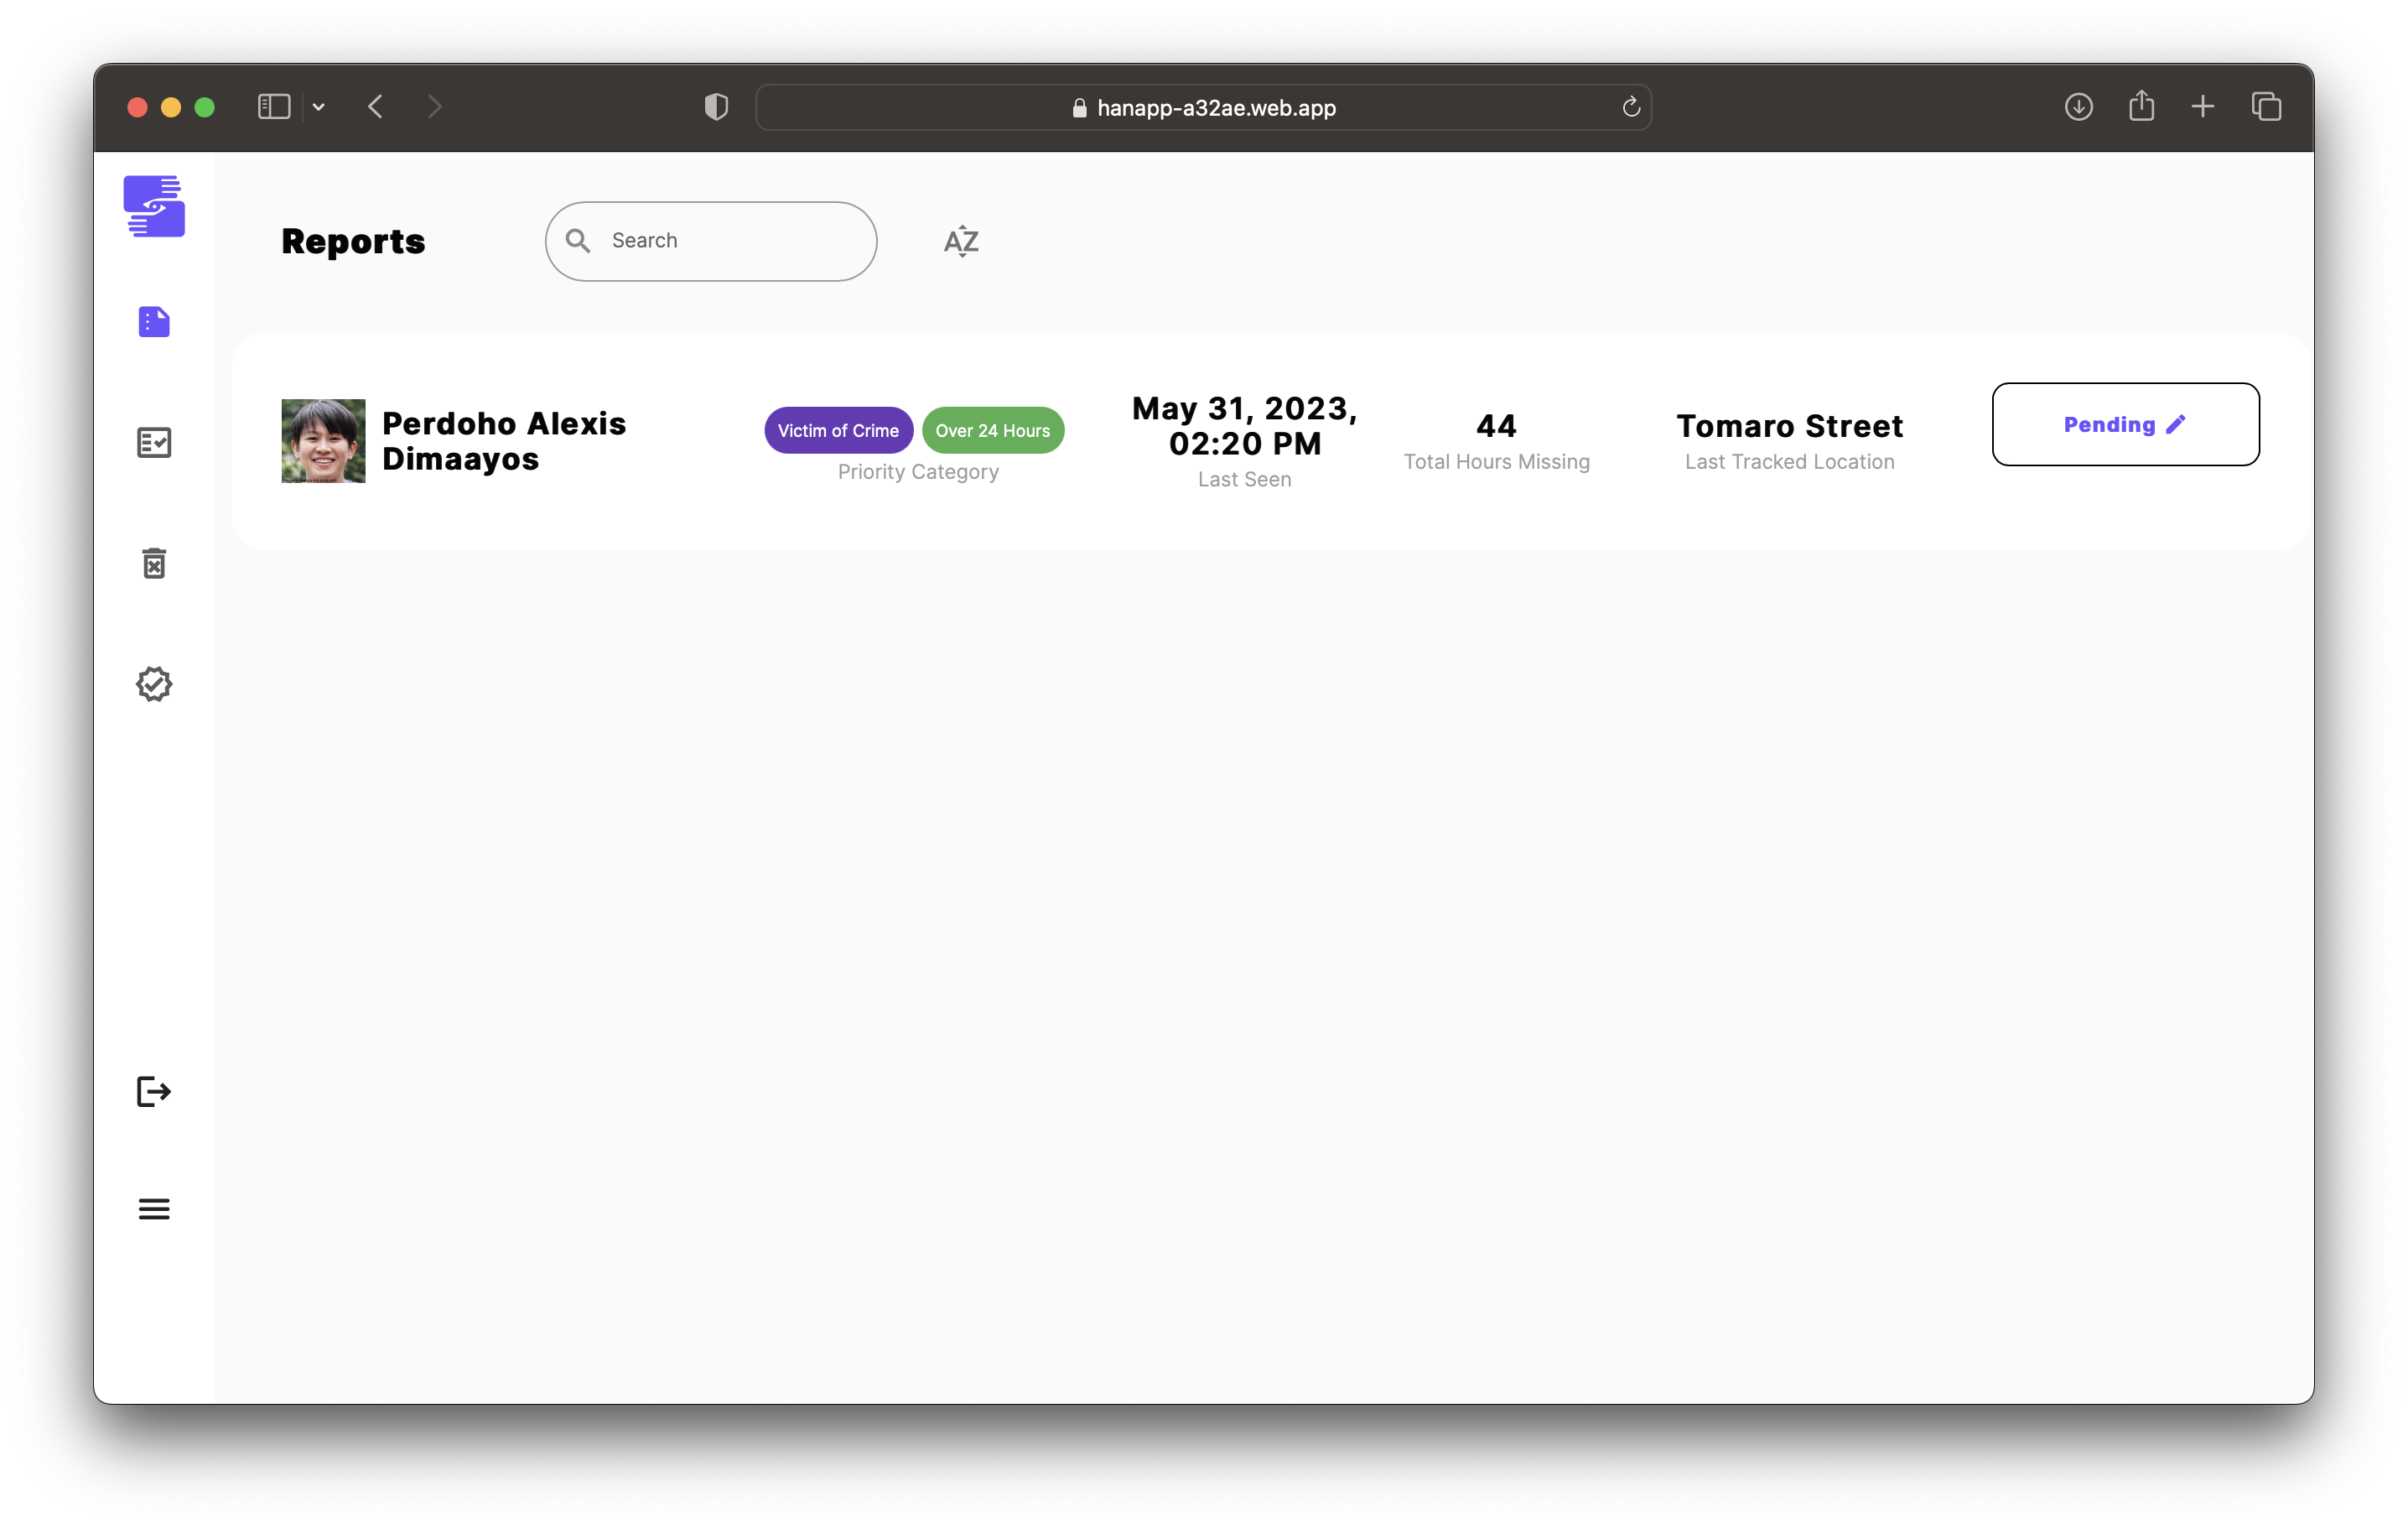
\includegraphics[scale=0.25]{figures/Chapter4/PNP/Pending.png}
    \caption{Admin Reports Management Suite View}
    \label{fig:PNP2}
\end{figure}
\subsection{PNP Admin Reports Management Suite}

Figure \ref{fig:PNP2} is the management suite for the PNP to access reports. The Reports page will have a scrollable list that will consist of the various details such as MP’s name, status of the report, time and date reported, and the location of MP. As for the status, a dropdown menu will be used to categorize each report namely, Received, Already Found, Verify Report, and Reported. For better management, reports are correctly being filtered into their respective statuses onto the different menus as seen on the left-hand side of the interface (i.e. verified reports will be on the verified menu).

\begin{figure}[!h]
    \centering
    \begin{subfigure}[c]{1\linewidth}
        \centering
        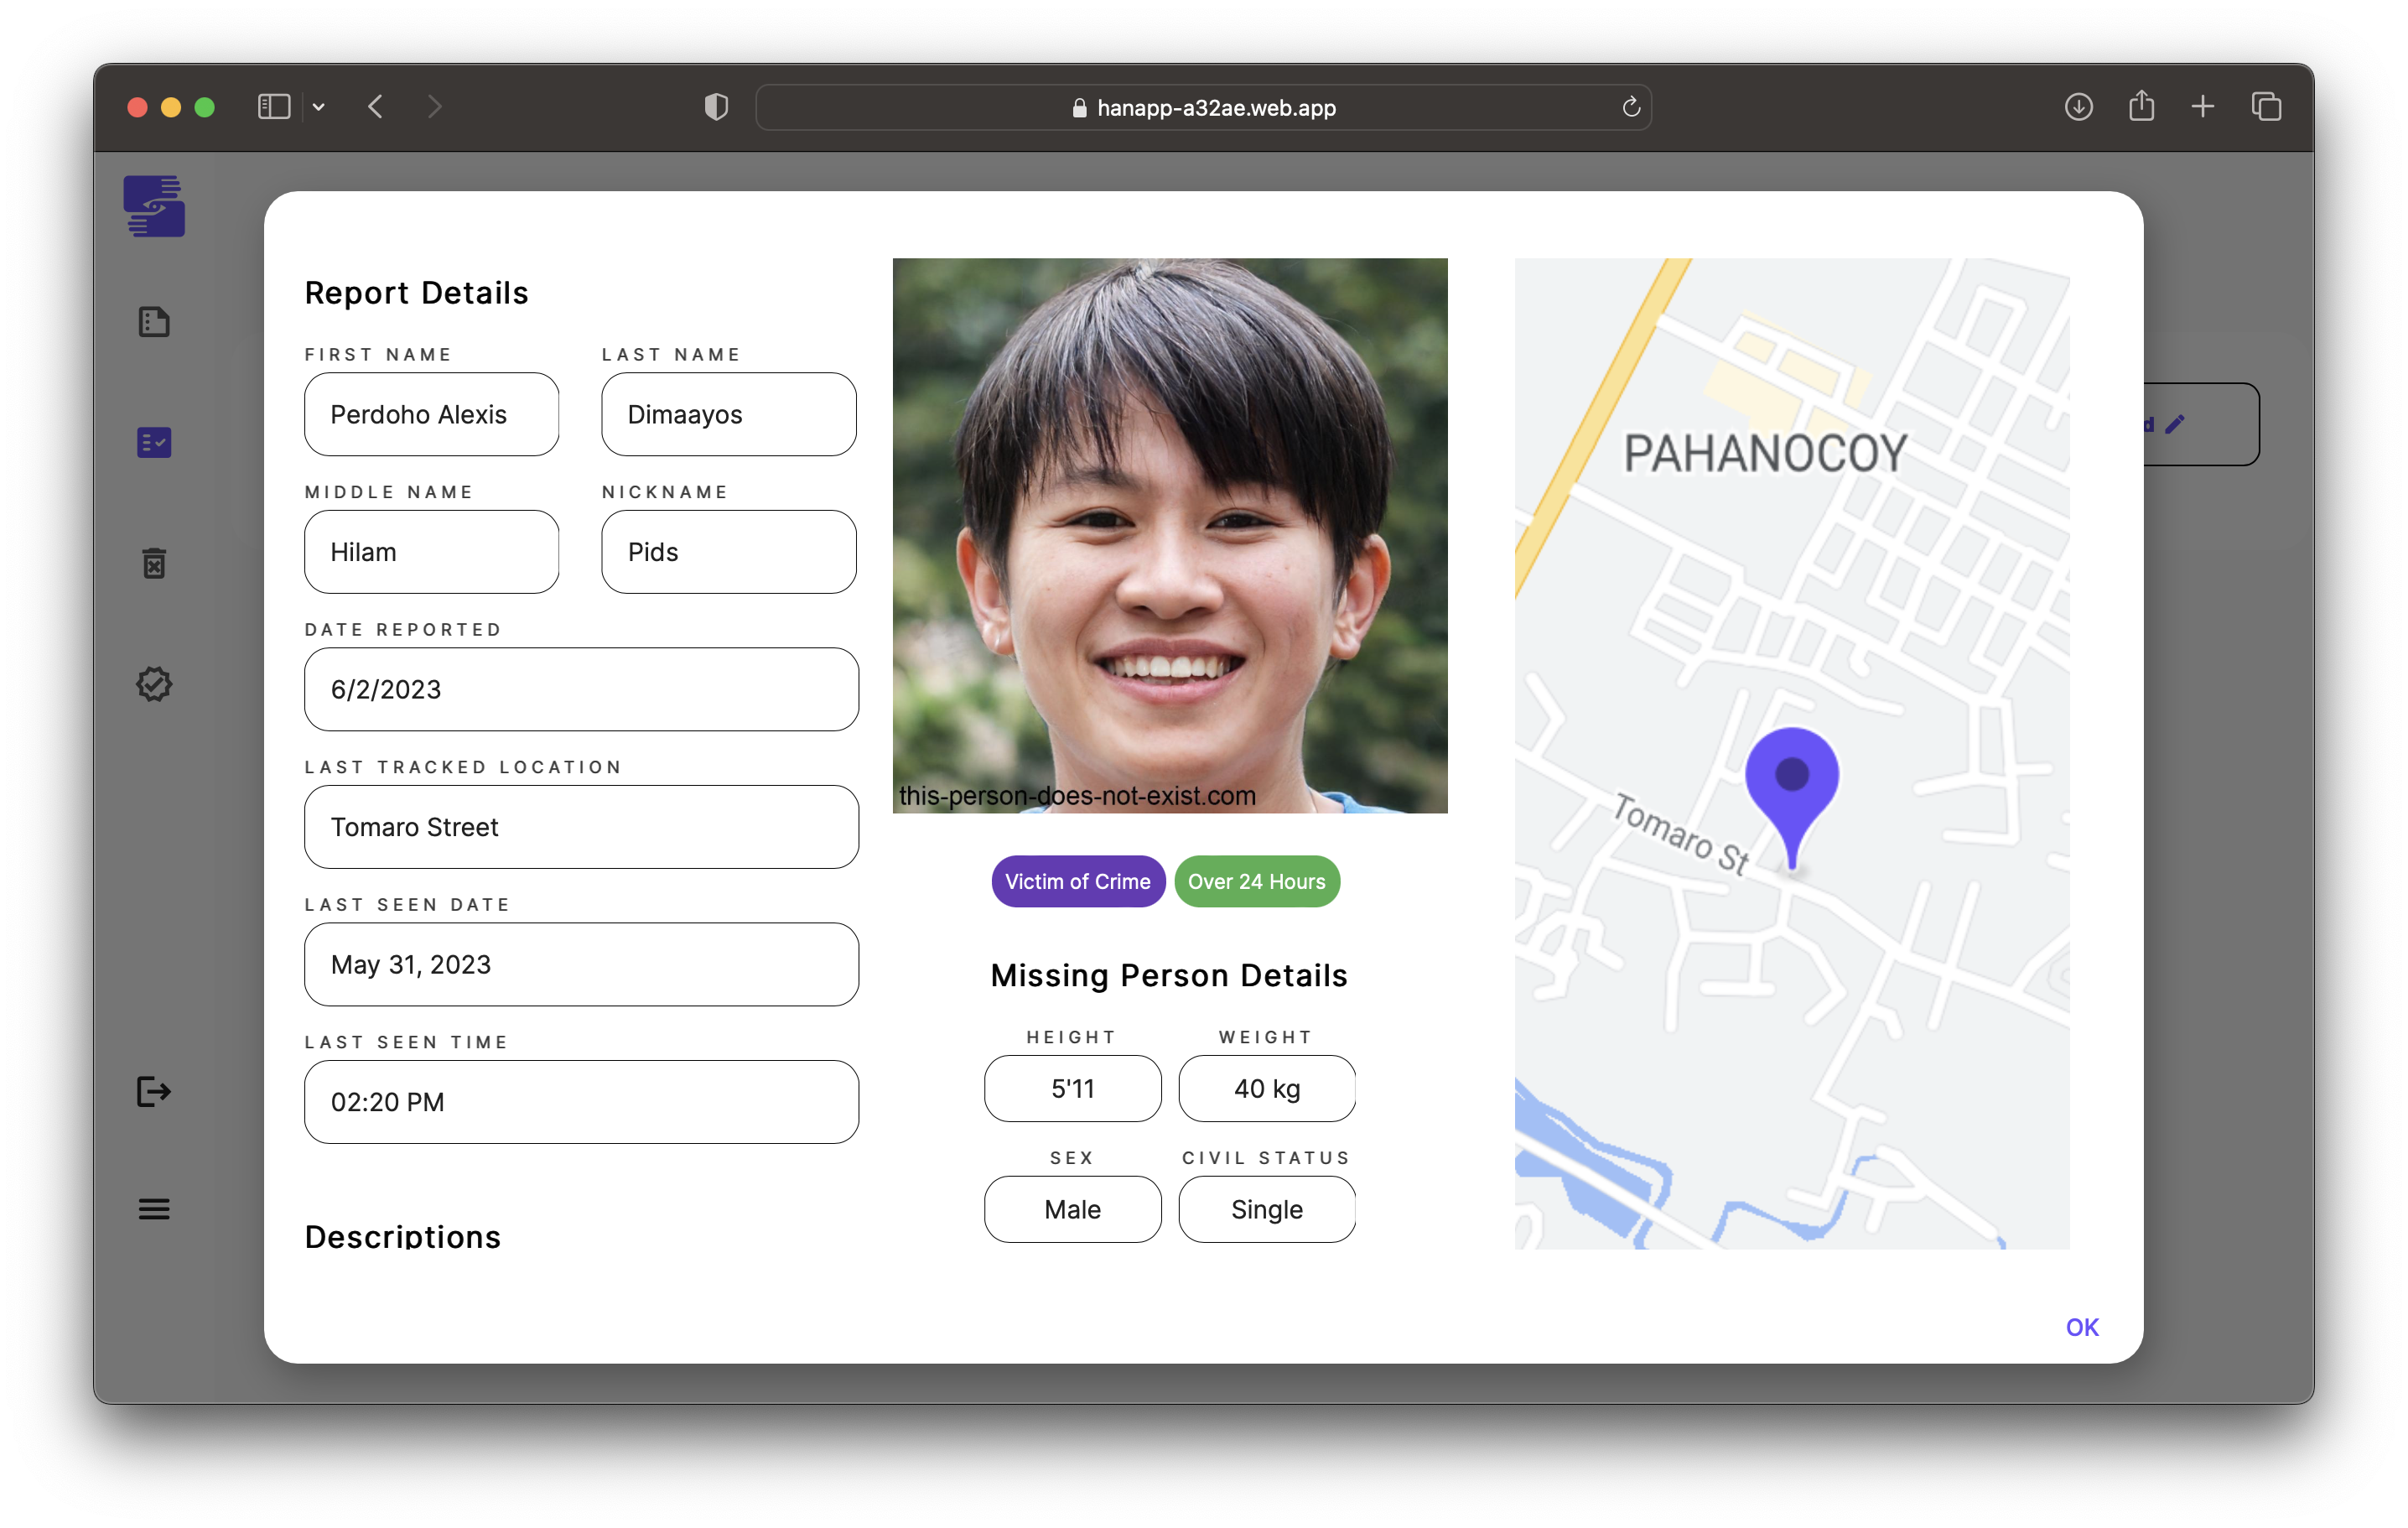
\includegraphics[scale=0.25]{figures/Chapter4/PNP/CaseView-1.png}
    \end{subfigure}
    \caption{Case View of Missing Person}
    \label{fig:reportDetails}
\end{figure}

\subsubsection{Viewing Report Details}

The report dialog box details the list of the necessary information that the reportee provided. Figure \ref{fig:reportDetails} illustrates missing person's descriptions, last seen location snapshot, and their picture that will be shown first to ease the process of identification. It is important to note that these are all the same and exact information required by the PNP when filing or verify a report of the missing person as per their guidelines on handling missing persons cases \cite{NationalPoliceCommission}. But compared to the numerous forms required in their guidelines, the details are more compact and summarized for their convenience. The data can be retrieved from the database through shared preferences plugin used.

\section{User or Main Interface}
The main interface will be subdivided into three various parts to cover all the features that was built throughout the process.

\subsection{User Registration, Authentication, and Login}
Authentication is necessary for the user-side. Figures \ref{fig:userLogin} and \ref{fig:userRegister} are the Login and Register page, respectively. Input fields will be provided for the registration such as email address, full name, sex, birth date, and a numeric input field will be observed for the phone number. To ensure that the user understands the Terms and Conditions and Privacy Policy, a hyperlinked text can be used to redirect them for their perusal. Then a register button will let the user account be registered and store in the database for authentication purposes.
\begin{figure}[!h]
    \centering
    \begin{minipage}[c]{0.50\linewidth}
        \centering
        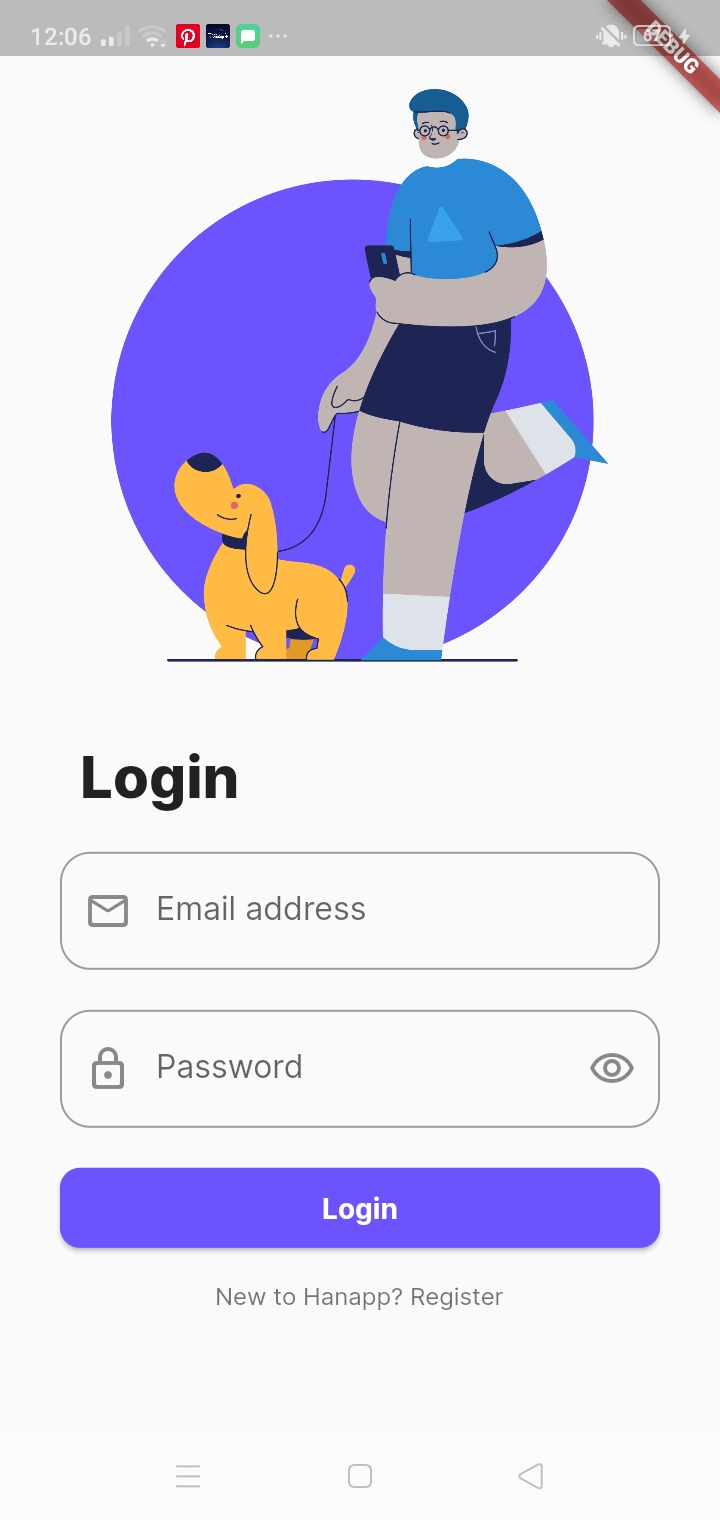
\includegraphics[scale=0.15]{figures/Chapter4/Main/Login.jpg}
        \caption{Login Page}
        \label{fig:userLogin}
    \end{minipage}
\end{figure}

In order to validate the authentication processes, use-case testing was initiated. The functionality of logging in meets the user requirement for a happy path since the expected output was observed. In order to mitigate any erroneous instances of unexpected outcome, incorrect credentials was utilized and as expected, the application will deter these circumstances.

\begin{figure}[!h]
    \centering
    \begin{subfigure}[c]{0.30\linewidth}
        \centering
        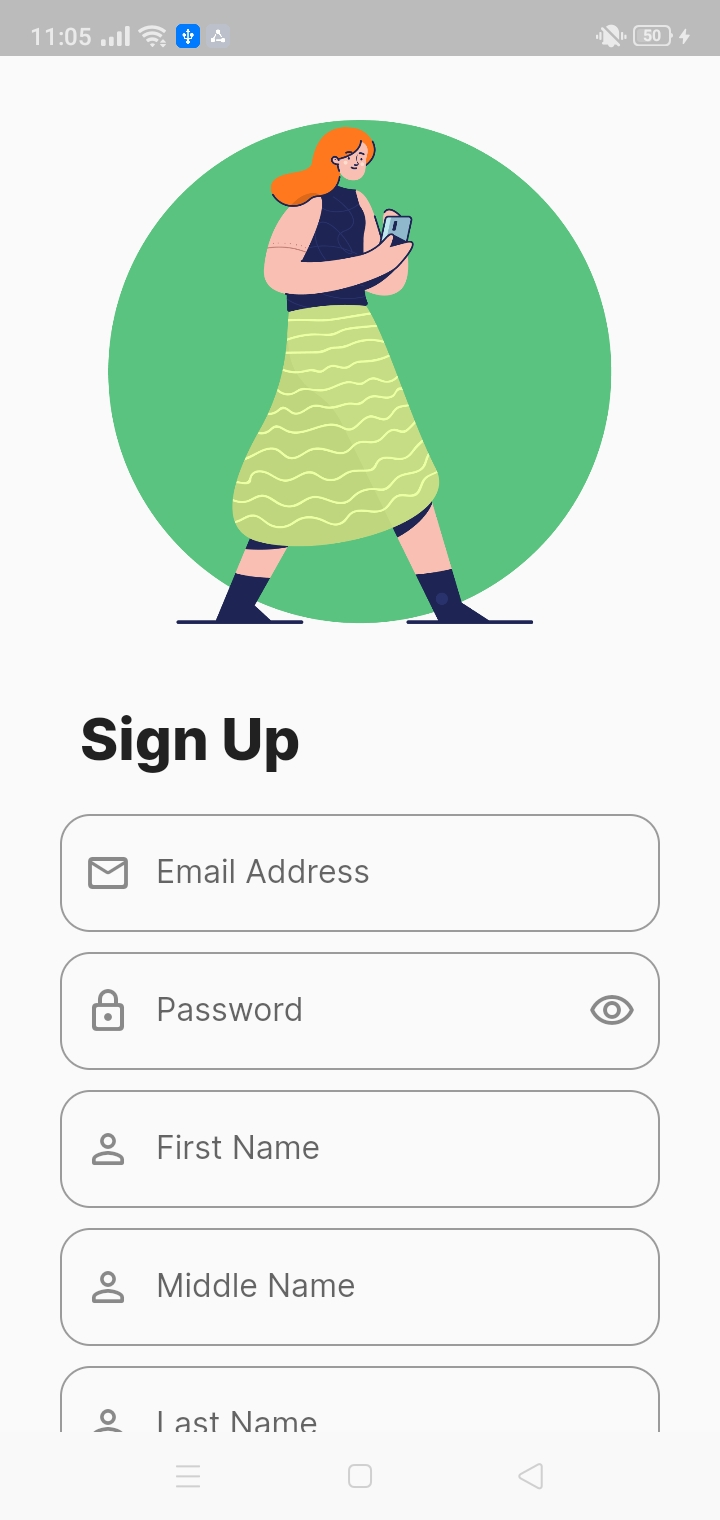
\includegraphics[scale=0.15]{figures/Chapter4/Main/SignUp-1.jpg}
    \end{subfigure}
    \centering
    \begin{subfigure}[c]{0.30\linewidth}
        \centering
        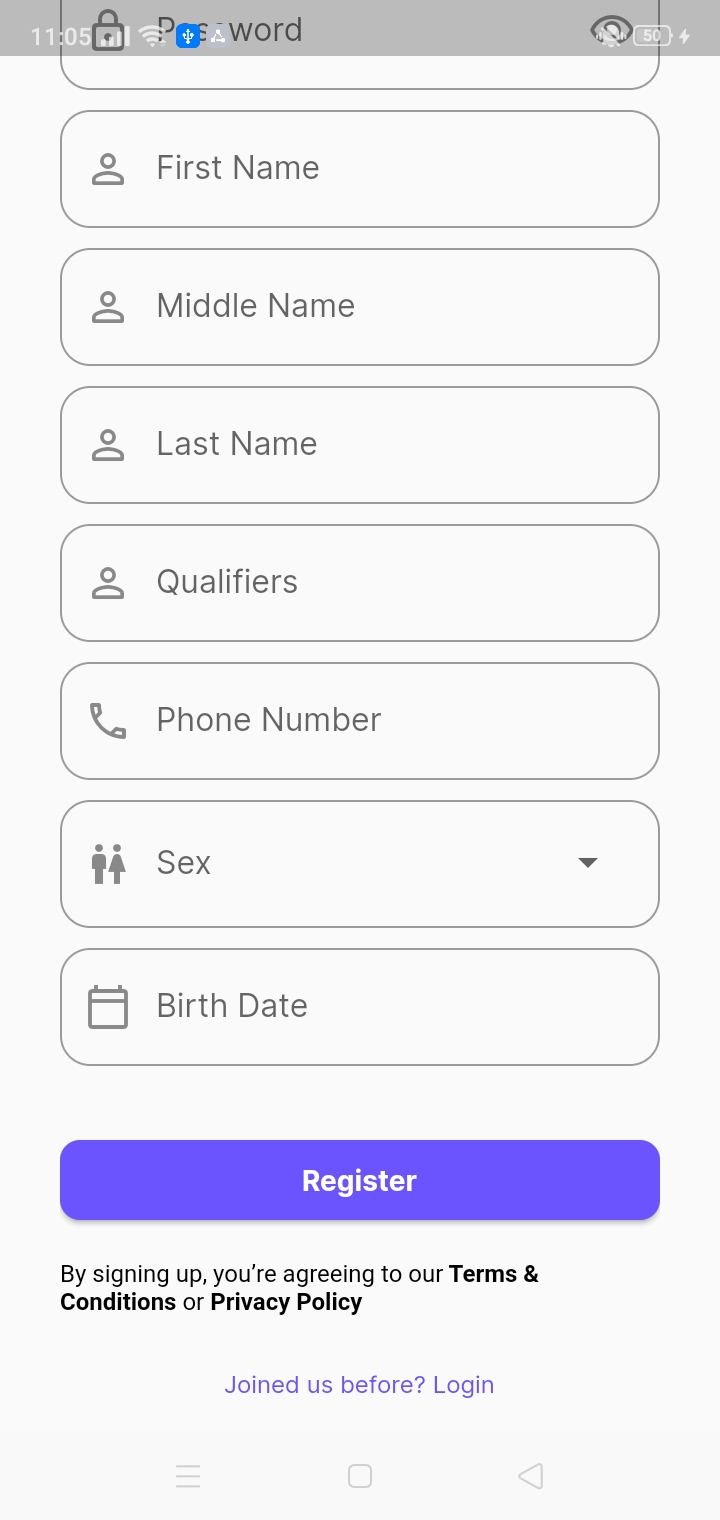
\includegraphics[scale=0.15]{figures/Chapter4/Main/SignUp-2.jpg}
    \end{subfigure}
    \caption{Sign Up Page}
    \label{fig:userRegister}
\end{figure}

\begin{figure}[!h]
    \centering
    \begin{subfigure}[c]{0.30\linewidth}
        \centering
        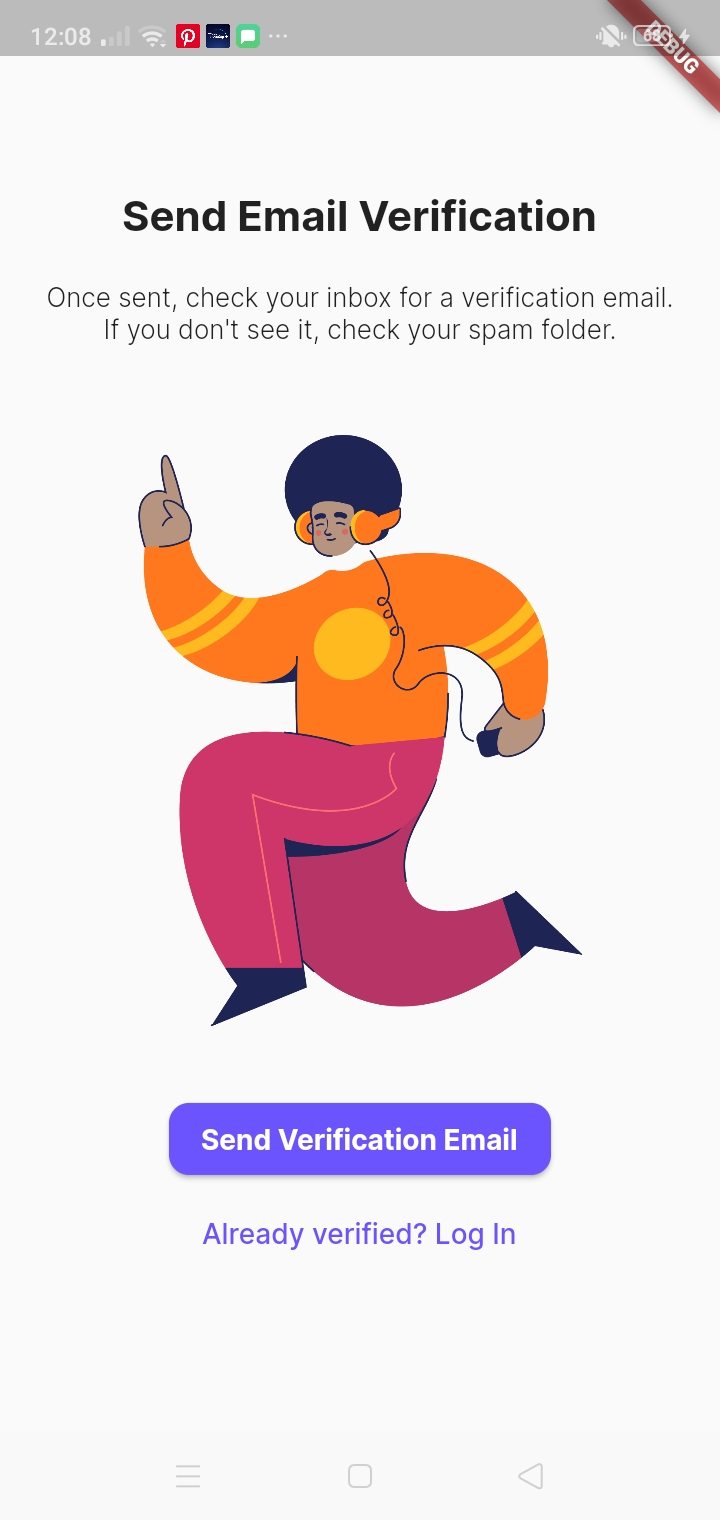
\includegraphics[scale=0.15]{figures/Chapter4/Main/Verification-1.jpg}
    \end{subfigure}
    \centering
    \begin{subfigure}[c]{0.30\linewidth}
        \centering
        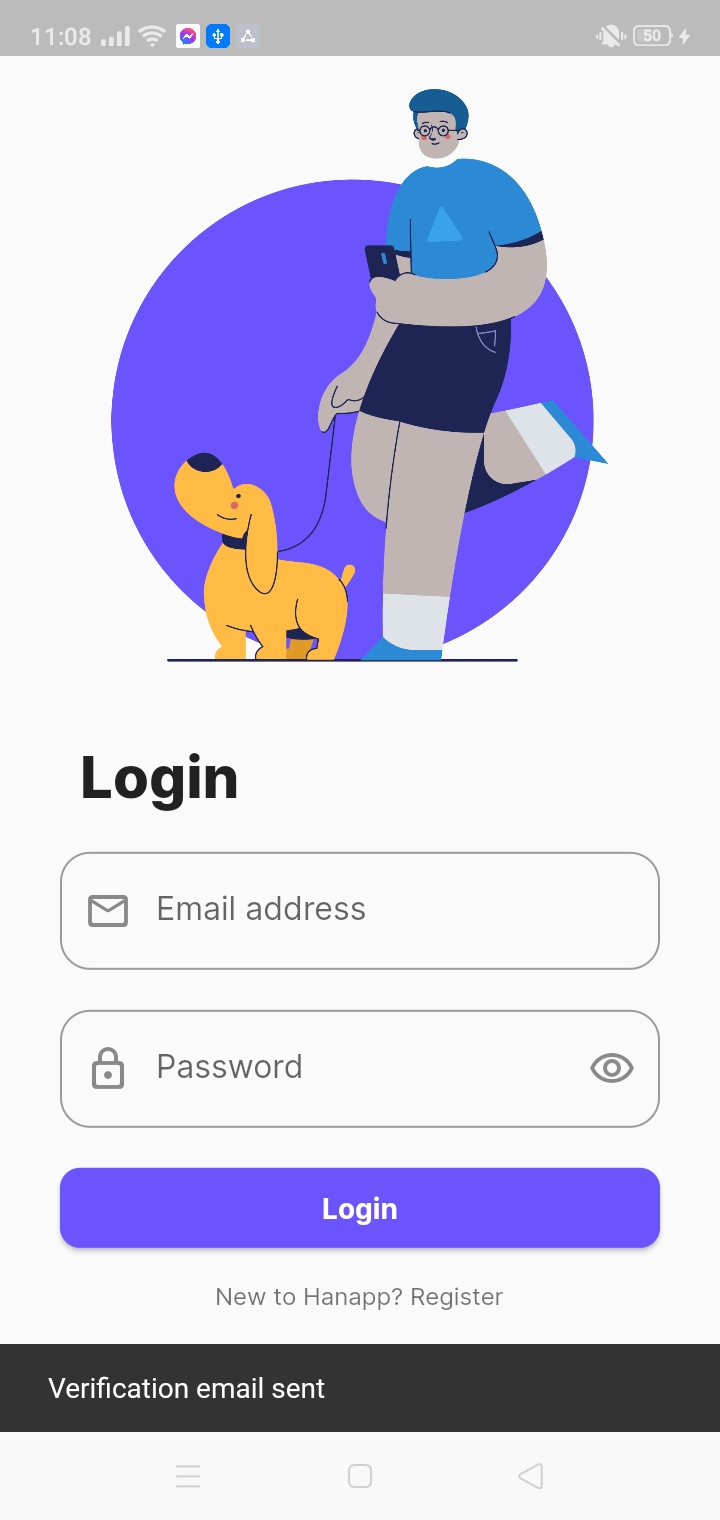
\includegraphics[scale=0.15]{figures/Chapter4/Main/Verification-2.jpg}
    \end{subfigure}
    \centering
    \begin{subfigure}[c]{0.30\linewidth}
        \centering
        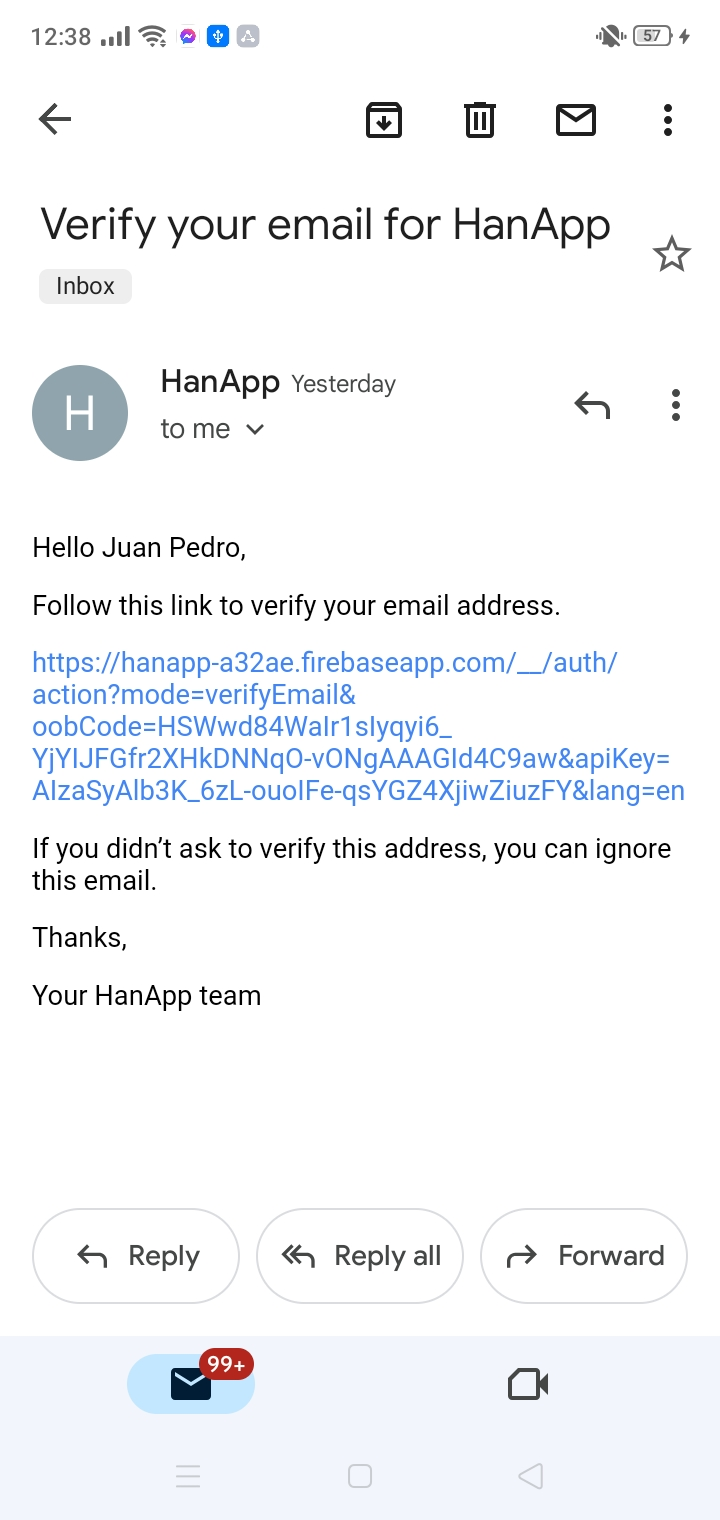
\includegraphics[scale=0.15]{figures/Chapter4/Main/Verification-3.jpg}
    \end{subfigure}
    \caption{Account Verification Process}
    \label{fig:accountVerification}
\end{figure}

\subsubsection{Account Verification}
In order to make sure that newly registered accounts are of human-origin and are legit accounts of potential users, accounts need to be authenticated first before being able to login. Figure \ref{fig:accountVerification}   illustrates the process of verification: first, after the user is registered, they will be redirected to a page where they will be given the choice to send email verification onto their newly registered email address for the application, or to redirect to the login page instead. If users select the option to send the verification email, they can then check their respective emails that ask for verification that, after clicking the link in the email, would mark their registered accounts as verified, allowing them to be able to login. If in some cases that users will opt-out of sending the verification email right after being registered, they still will be met with the same verification page if they try to login with a none email-verified account. 

\begin{figure}[!h]
    \centering
    \begin{minipage}[c]{0.40\linewidth}
        \centering
        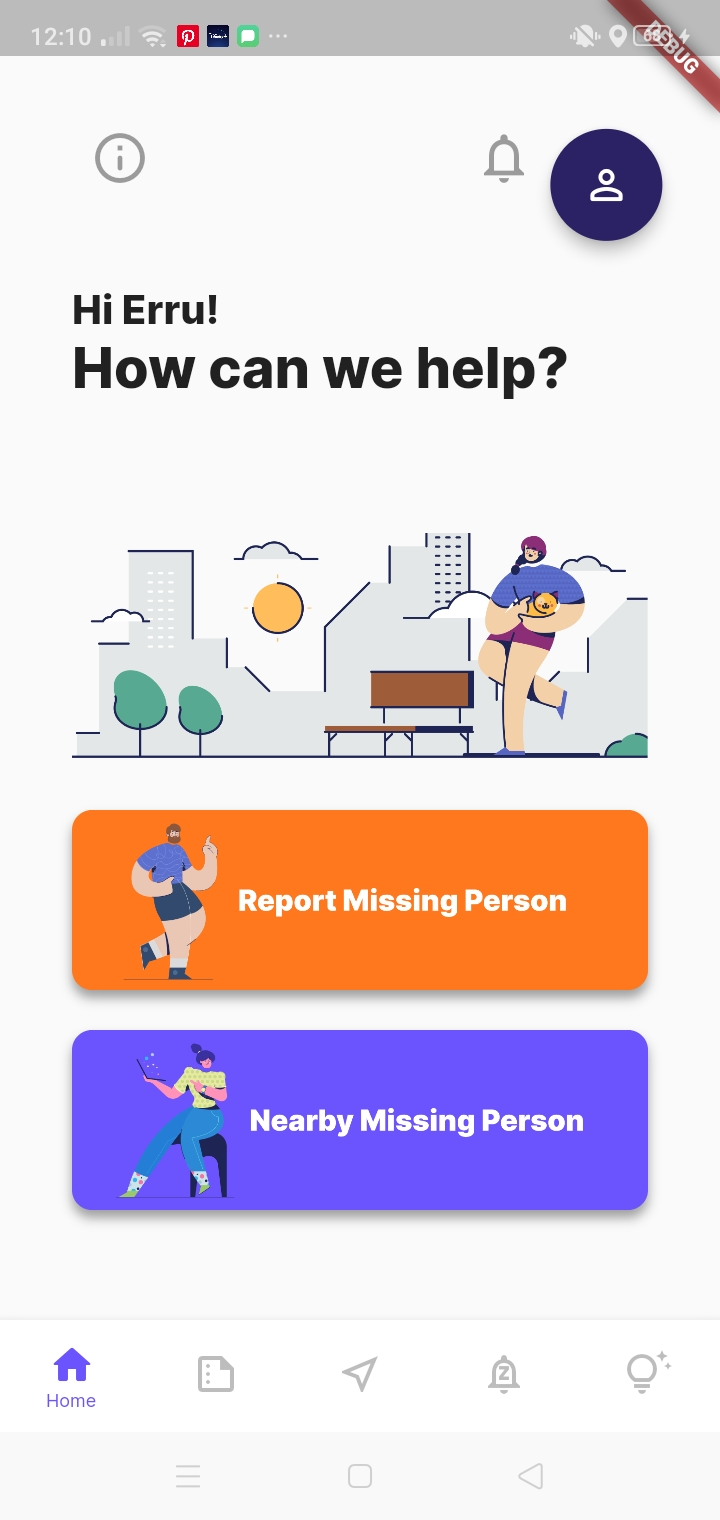
\includegraphics[scale=0.15]{figures/Chapter4/Main/Home.jpg}
        \caption{Home Page}
        \label{fig:userHome}
    \end{minipage}
    \centering
    \begin{minipage}[c]{0.40\linewidth}
        \centering
        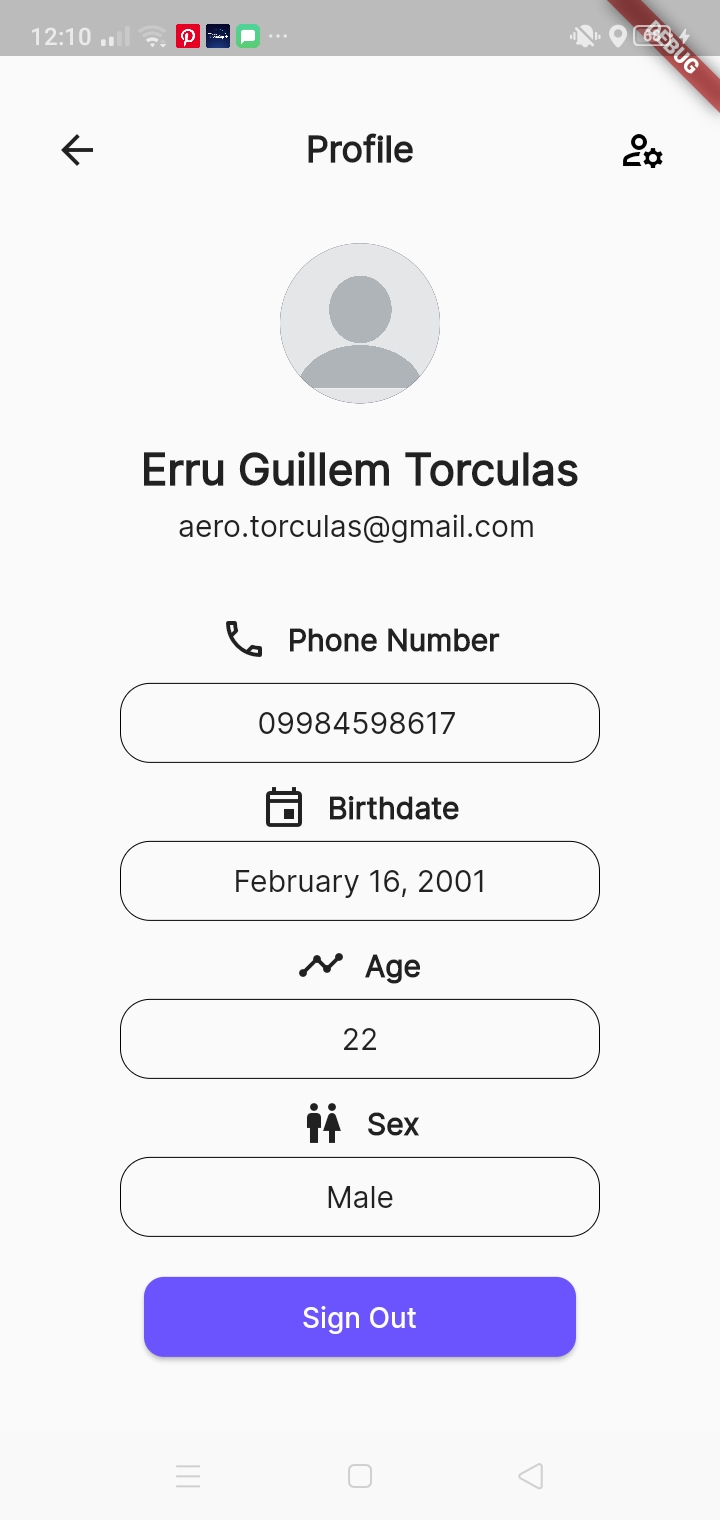
\includegraphics[scale=0.15]{figures/Chapter4/Main/Profile.jpg}
        \caption{Profile Page}
        \label{fig:userProfile}
    \end{minipage}
\end{figure}
Moreover, when user authentication is completed, the login button will let them proceed to the Home page of the application where the user will have two options: Report Missing or Nearby Missing persons as shown in \ref{fig:userHome}. This will allow the user to optimally choose what course of action are they going to take on by presenting these call to action button first. A bottom navigation bar will be visible throughout the user’s interaction of the app assuring that they can easily navigate the entire features offered to them. The navigation bar will consist of five (5) sections, namely, Home, Reports, Nearby, Notifications, and Updates. Each section will be utilized to build the features of the app and functions specifically to the needs of the user. Figure \ref{fig:userProfile} illustrates the profile page that will consist of the details about the user that was already pre-filled on the registration part. Thus, it will display: the concatenated full name of the user, email address used in account registration, birth-date, age, and lastly sex. In addition, a sign out button will also be provided in case the user decided to log out from their account.


\subsection{Report Pages}

The Report page is one of the integral parts of this application that would allow users to give necessary information in the event of a person missing. It streamlines the reporting process done by the PNP and replicates their incident report, one that had to be done in written format in their respective outposts, so that verification is manageable \cite{NationalPoliceCommission}. Input text fields will be used throughout this page. Accompanying it with dropdown menus for categorical information such as Gender, and Blood type. Physical indicators will have mostly text/paragraph input fields for elaborations and additional details that are needed to disclose such as body marks, tattoos, and the like.

\subsubsection{Report Page 1: Classifiers}
\begin{figure}[!h]
    \centering
    \begin{minipage}[c]{0.50\linewidth}
        \centering
        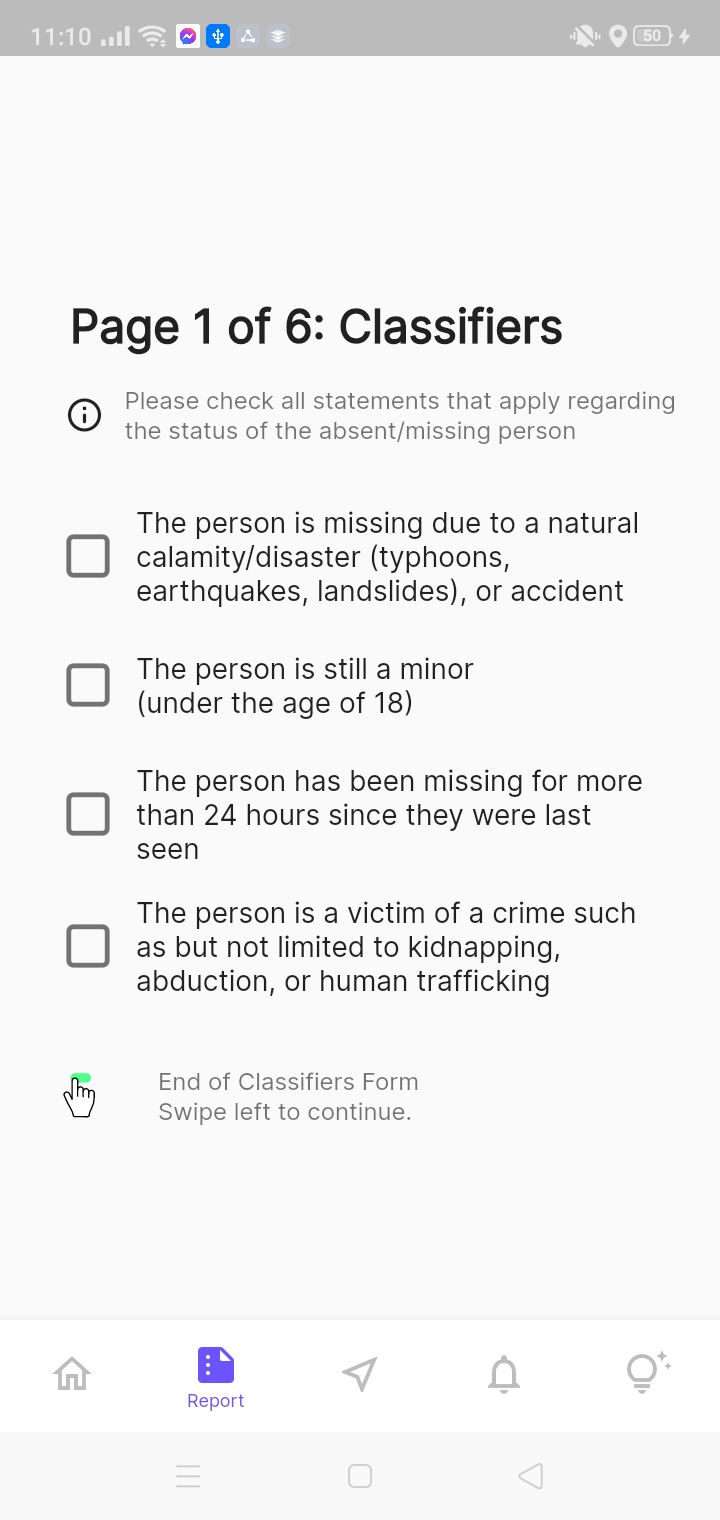
\includegraphics[scale=0.15]{figures/Chapter4/Main/p1.jpg}
        \caption{Report Form Page 1}
        \label{fig:p1}
    \end{minipage}
\end{figure}

On the first page of the reports section as seen in figure \ref{fig:p1}, the categorization of the missing person being reported is located. The reporting user will be met with checkboxes indicating that their person being reported is (1) a person missing due to natural calamities, (2) a person under the age of 18, and is therefore classified as a minor, (3) a person that has been missing for over 24 hours already, or lastly, (4) a person that is a victim of a crime such as, but not limited to, kidnapping, human trafficking, etc.

\subsubsection{Report Page 2: Reportee Details}

\begin{figure}[!h]
    \centering
    \begin{subfigure}[c]{0.30\linewidth}
        \centering
        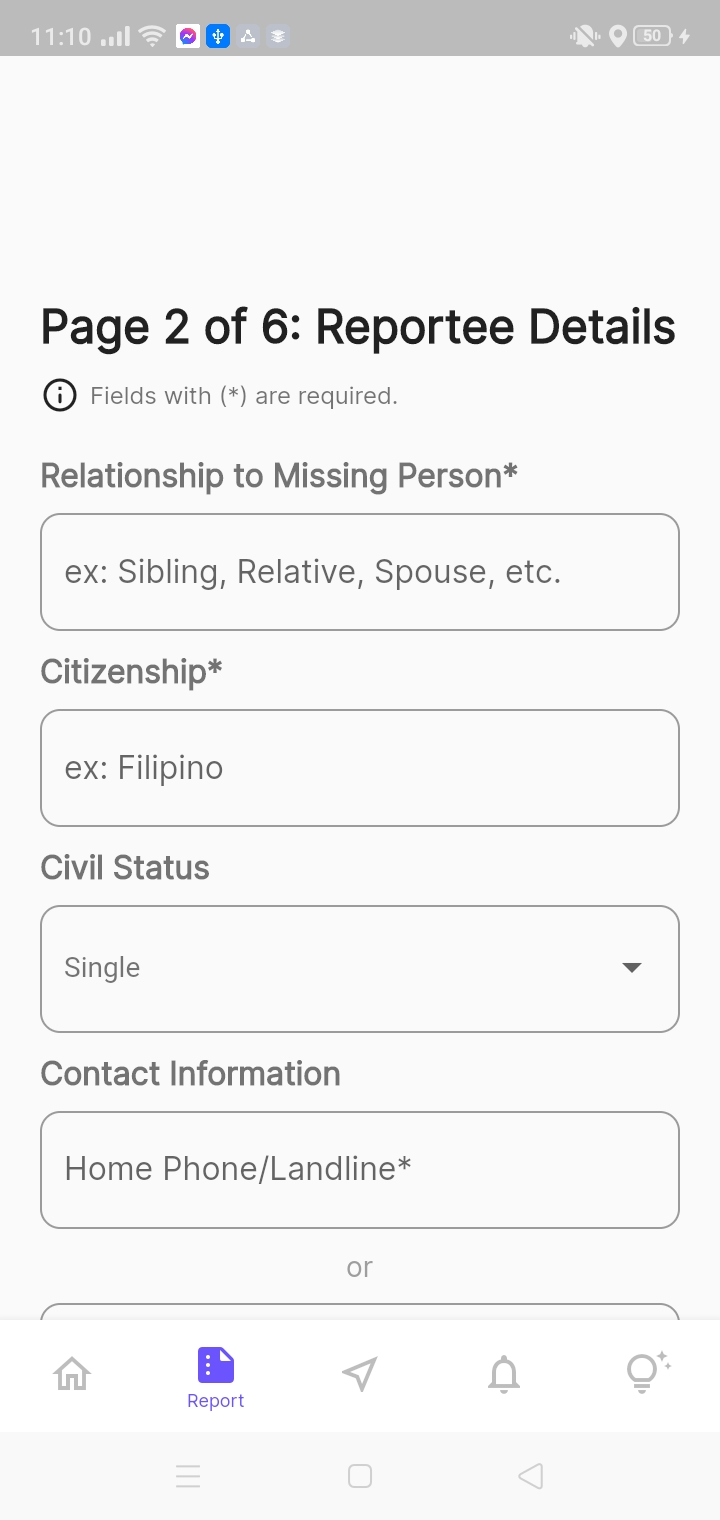
\includegraphics[scale=0.15]{figures/Chapter4/Main/p2-1.jpg}
    \end{subfigure}
    \centering
    \begin{subfigure}[c]{0.30\linewidth}
        \centering
        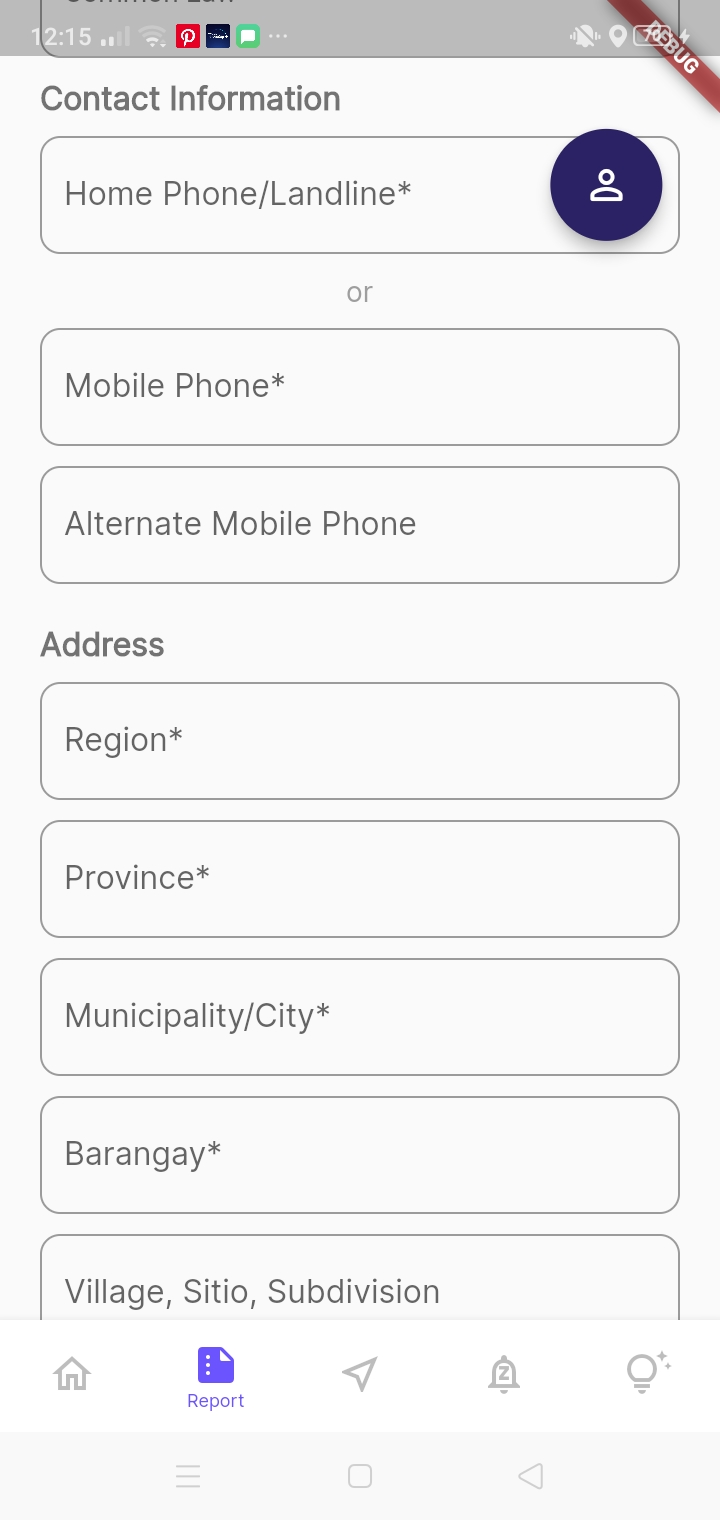
\includegraphics[scale=0.15]{figures/Chapter4/Main/p2-2.jpg}
    \end{subfigure}
    \centering
    \begin{subfigure}[c]{0.30\linewidth}
        \centering
        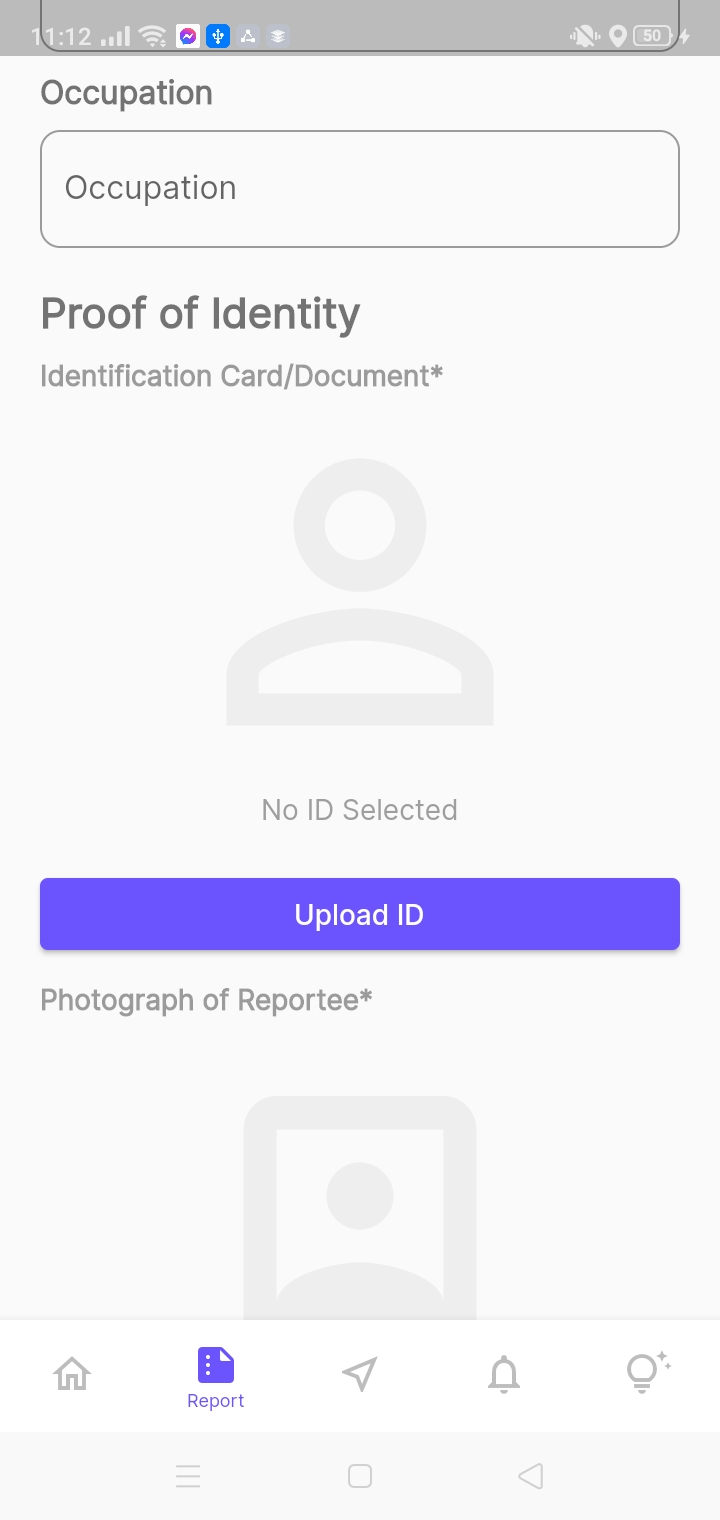
\includegraphics[scale=0.15]{figures/Chapter4/Main/p2-3.jpg}
    \end{subfigure}
    \caption{Report Form Page 2}
    \label{fig:ReportPage2}
\end{figure}

On the second page of the reports page, as seen in figure \ref{fig:ReportPage2}, the reportee will be asked to fill out required information about them. This includes the reportee's relationship to the missing person, contact information, address, citizenship, and the proofs of identity through a picture of his/her identification card (ID), and a selfie. The selfie serves as a secondary authentication measure in lieu of reporting remotely rather than in person, and also allows the PNP to verify if the user's face matches that of the photo in their submitted ID. The reportee's basic information such as name, birth-date, age, and sex are no longer required to be re-entered since they are now already found in the user's profile. 

\textbf{List of Valid IDs}. In Report Page 2, to avoid confusion when submitting reportee IDs as proof of identity and minimize issues during report verification by the PNP, it is imperative to provide the reportee with a list of Valid IDs that are required by the PNP when filing a report. The list is shown when the users tap the ``information" (i) icon seen in Figure \ref{fig:ReportPage2} under proof of identity, while the pop-up dialogue enumerating the list of Valid IDs is shown in Figure \ref{fig:validIDs}.

The list of Valid IDs include government-issued IDs or other IDs (such as work or school IDs) that should at least have the reportee's name, photo, and birth date for verification purposes. If the user does not have their ID at the moment of filling out the report, they can make use of the ``Save as Draft" feature to allow them to upload their ID at a later time once available.
\begin{figure}[!h]
    \centering
    \begin{subfigure}[c]{0.40\linewidth}
        \centering
        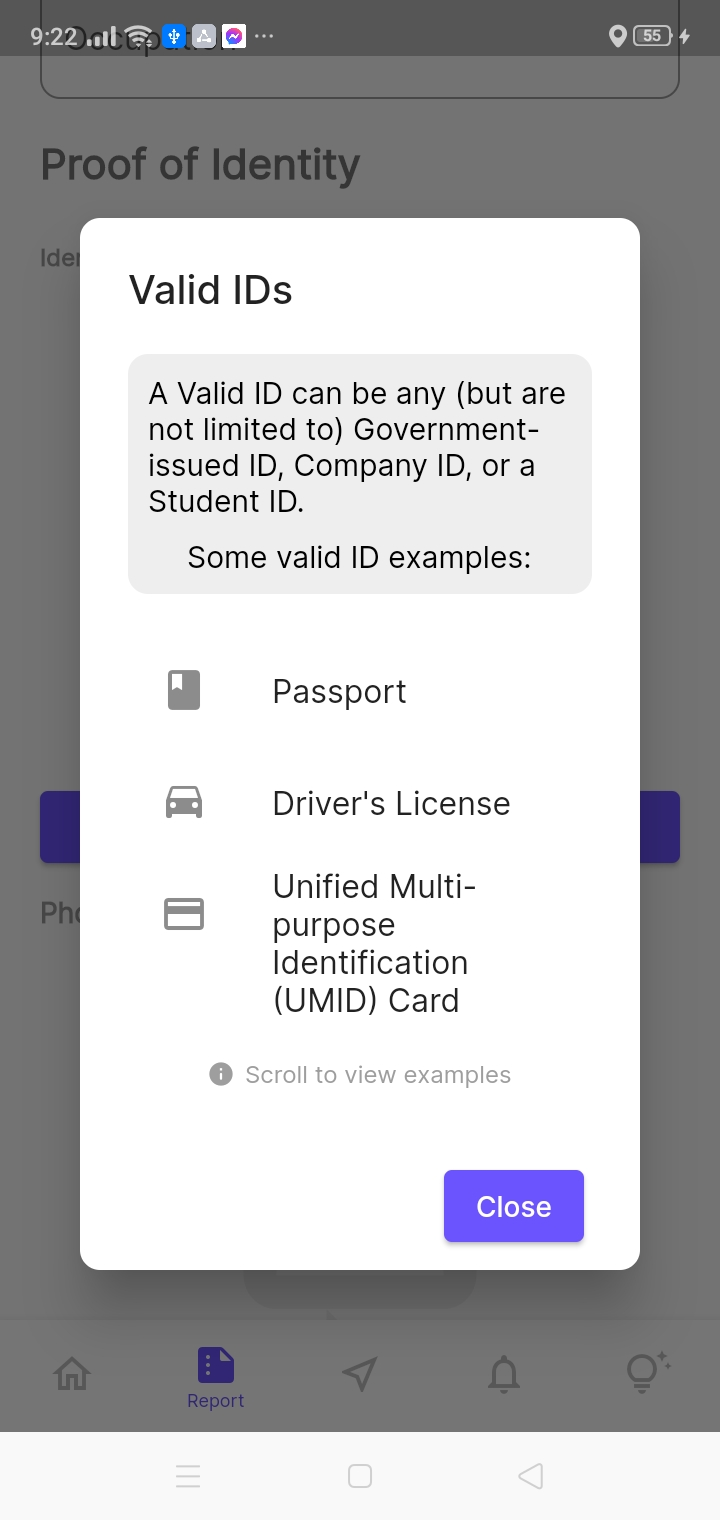
\includegraphics[scale=0.15]{figures/Chapter4/Main/validID.jpg}
    \end{subfigure}
    \caption{Valid IDs Information for Proof of Identity}
    \label{fig:validIDs}
\end{figure}

\subsubsection{Report Page 3: Absent/Missing Person Details}

The third page of the reports section, as seen in figure \ref{fig:ReportPage3}, requires the necessary information about the reported missing person such as their name, birth-date, sex, address, and contact information. It is important to note the specific usage of the term ``Absent/Missing Person" as it is the same term used in PNP's required forms when handling missing persons cases, specifically ``Annex C: Checklist for Absent/Missing Person".

\begin{figure}[!h]
    \centering
    \begin{subfigure}[c]{0.30\linewidth}
        \centering
        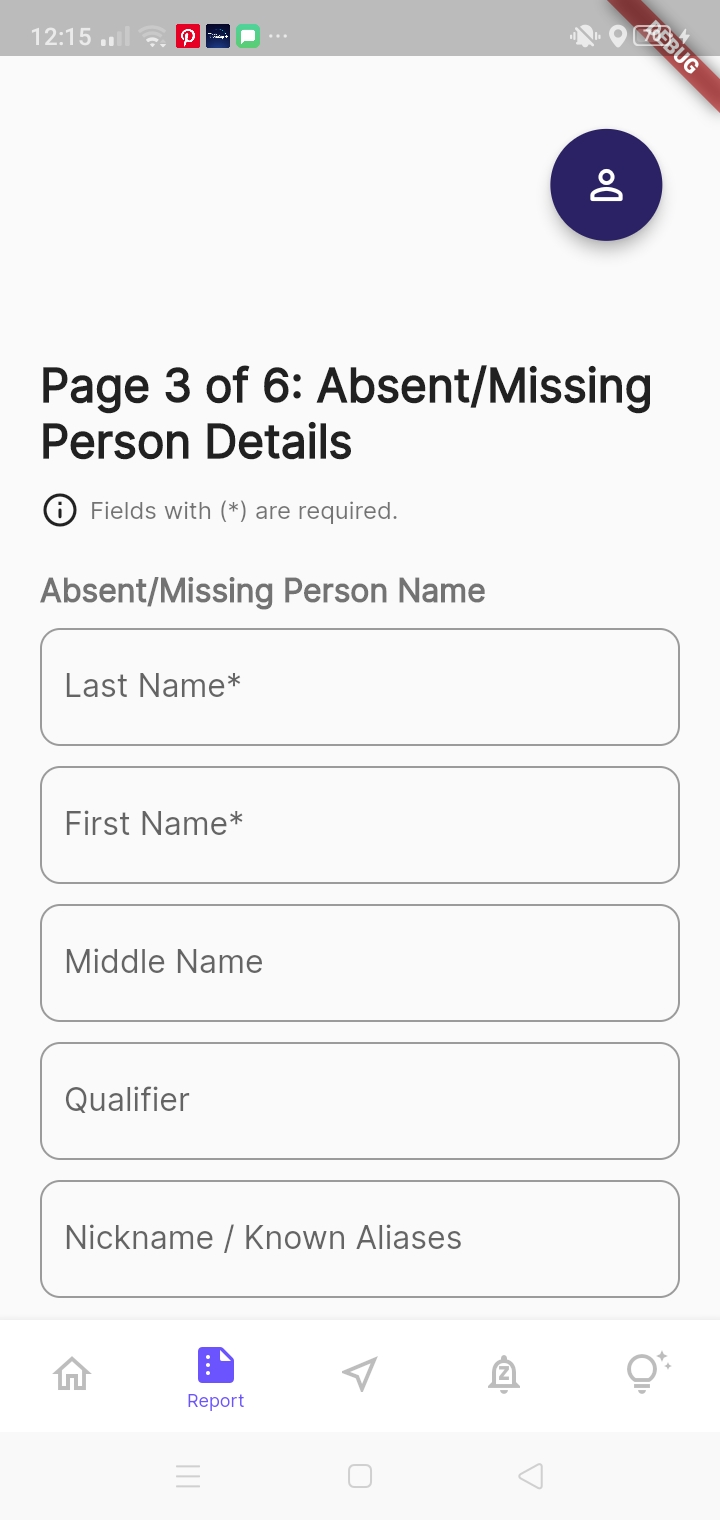
\includegraphics[scale=0.15]{figures/Chapter4/Main/p3-1.jpg}
    \end{subfigure}
    \centering
    \begin{subfigure}[c]{0.30\linewidth}
        \centering
        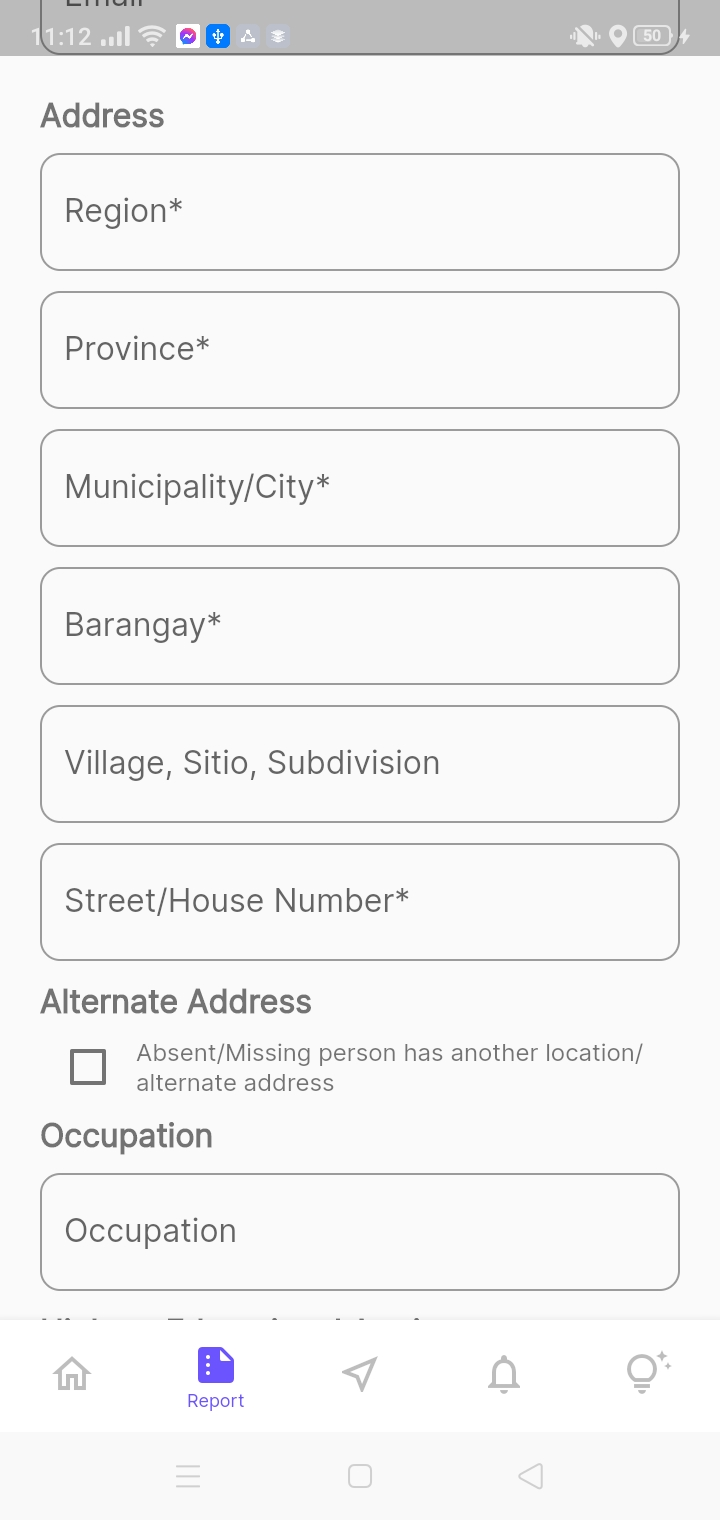
\includegraphics[scale=0.15]{figures/Chapter4/Main/p3-3.jpg}
    \end{subfigure}
    \centering
    \begin{subfigure}[c]{0.30\linewidth}
        \centering
        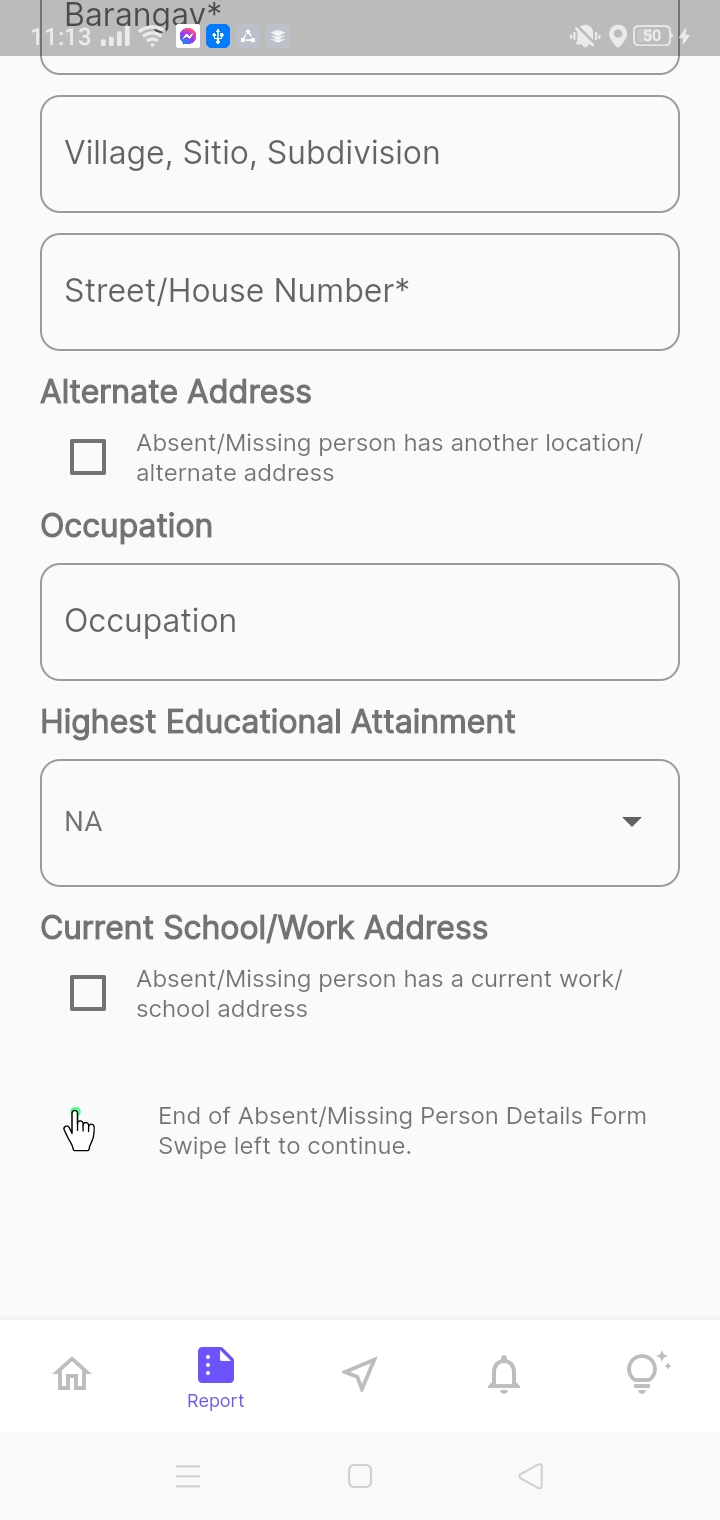
\includegraphics[scale=0.15]{figures/Chapter4/Main/p3-4.jpg}
    \end{subfigure}
    \caption{Report Form Page 3}
    \label{fig:ReportPage3}
\end{figure}

\subsubsection{Report Page 4: Absent/Missing Person Description}

The fourth page of the reports section, seen in figure \ref{fig:ReportPage4} still focuses on the information regarding the missing person. This time, however, are information relating to things that can most likely help strangers identify the missing person such as scars, marks, tattoos, hair color, eye color, prosthetic, birth defects, last known clothing and accessories, height, weight, blood type, medications, social media accounts, and of course, the last photograph of the missing person. Dental and Fingerprint records can also be added if the reportee wants to.

\begin{figure}[!h]
    \centering
    \begin{subfigure}[c]{0.30\linewidth}
        \centering
        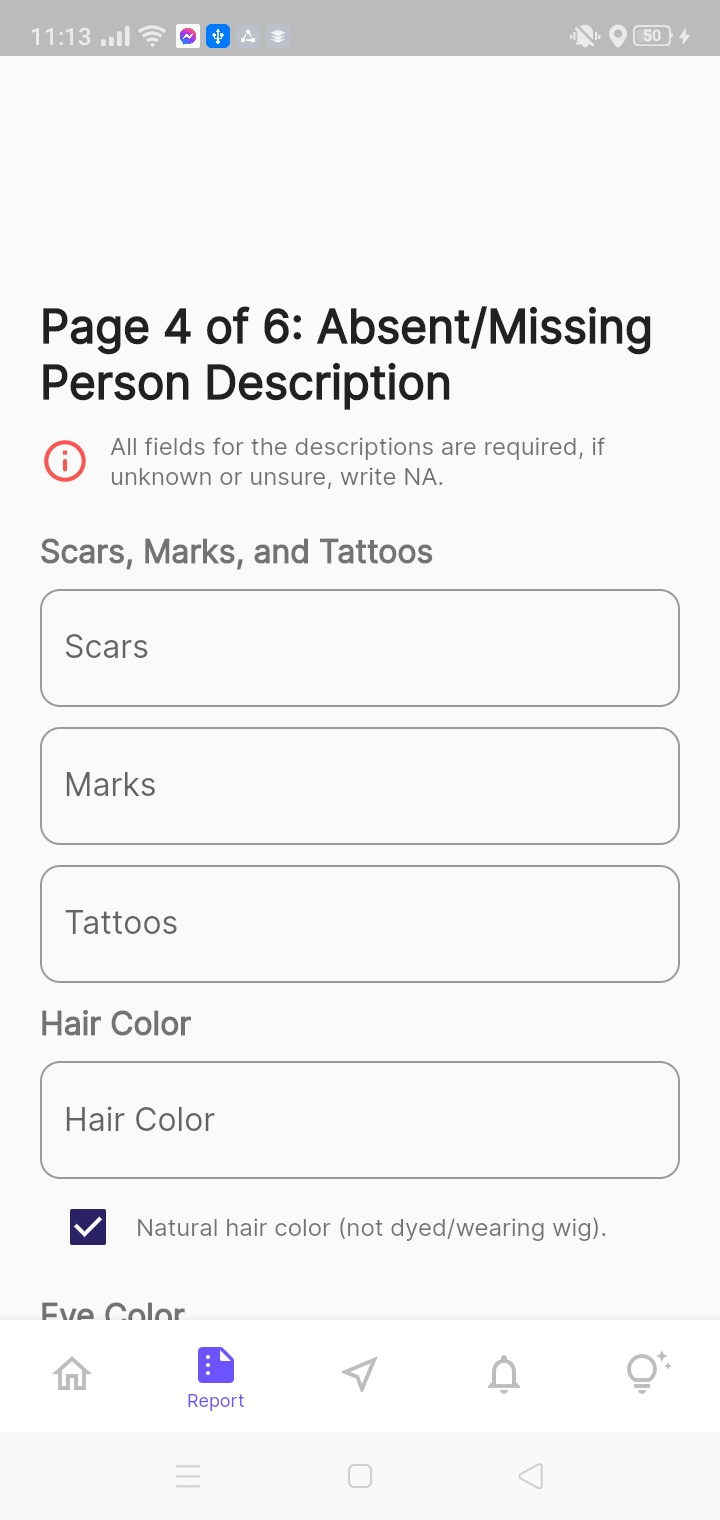
\includegraphics[scale=0.15]{figures/Chapter4/Main/p4-1.jpg}
    \end{subfigure}
    \centering
    \begin{subfigure}[c]{0.30\linewidth}
        \centering
        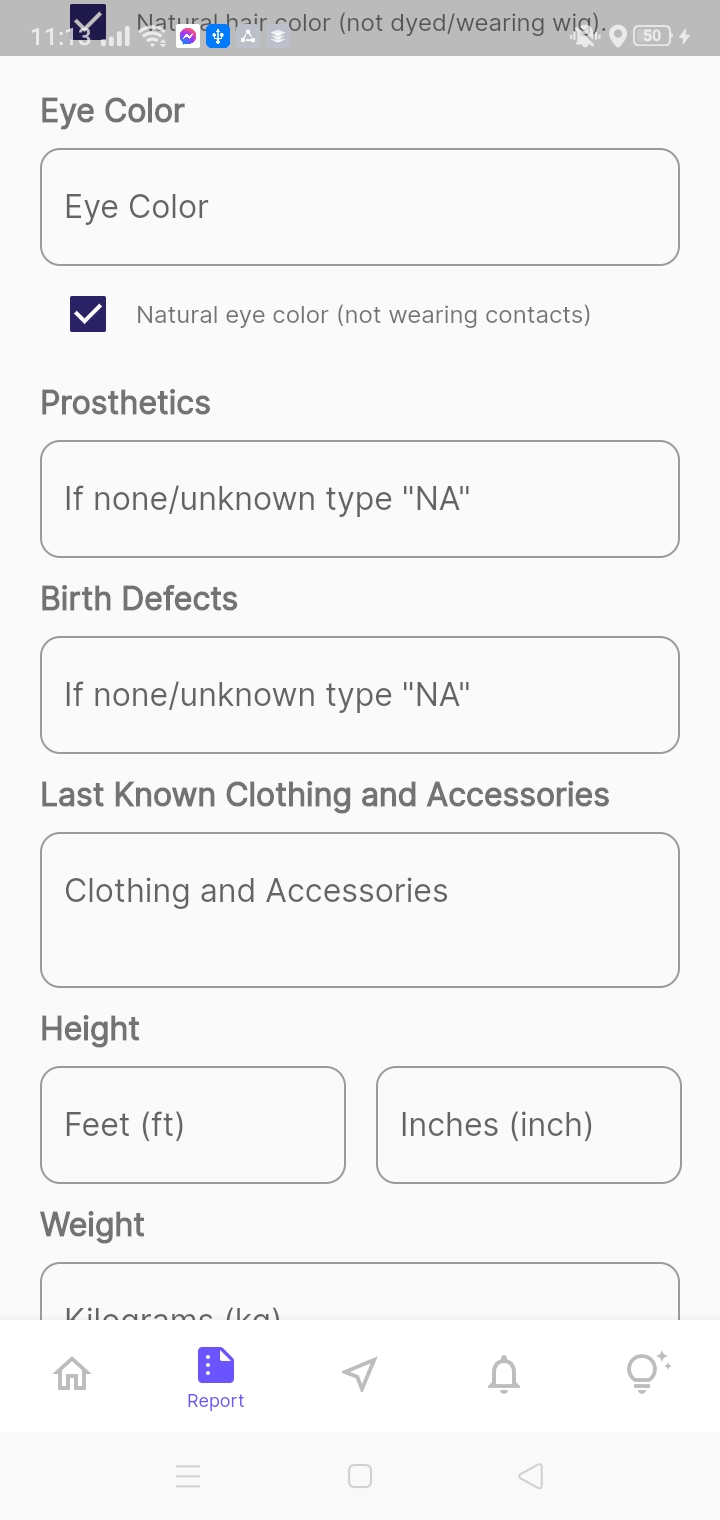
\includegraphics[scale=0.15]{figures/Chapter4/Main/p4-2.jpg}
    \end{subfigure}
    \centering
    \begin{subfigure}[c]{0.30\linewidth}
        \centering
        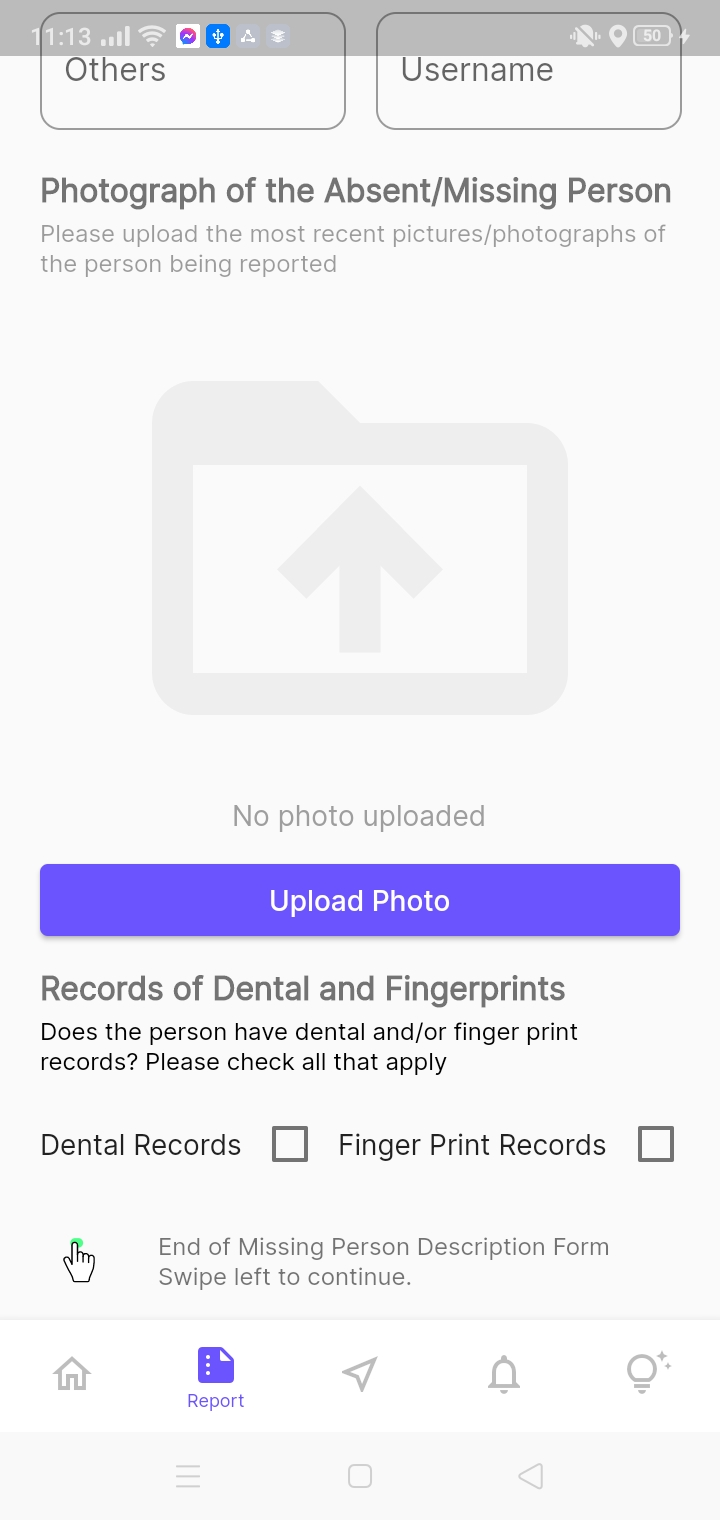
\includegraphics[scale=0.15]{figures/Chapter4/Main/p4-4.jpg}
    \end{subfigure}
    \caption{Report Form Page 4}
    \label{fig:ReportPage4}
\end{figure}

\subsubsection{Report Page 5: Incident Details}

The fifth page of the reports, as seen in figure \ref{fig:ReportPage5} requires information about the incident relating the disappearance of the missing person and is based on the ``Narrative of the Incident" section of the PNP's Incident Report Form which is used for reporting incidents including those of missing persons cases.

\begin{figure}[!h]
    \centering
    \begin{subfigure}[c]{0.30\linewidth}
        \centering
        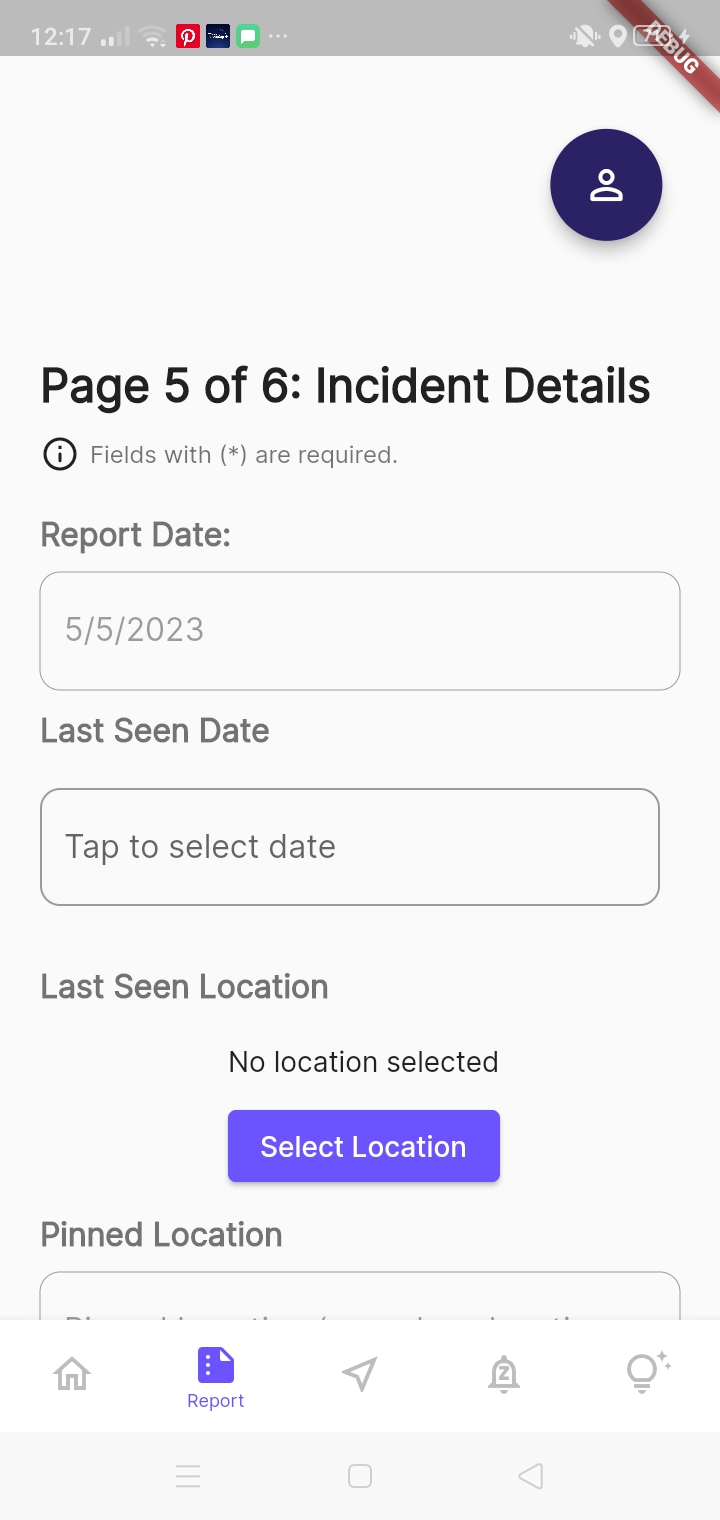
\includegraphics[scale=0.15]{figures/Chapter4/Main/p5-1.jpg}
    \end{subfigure}
    \centering
    \begin{subfigure}[c]{0.30\linewidth}
        \centering
        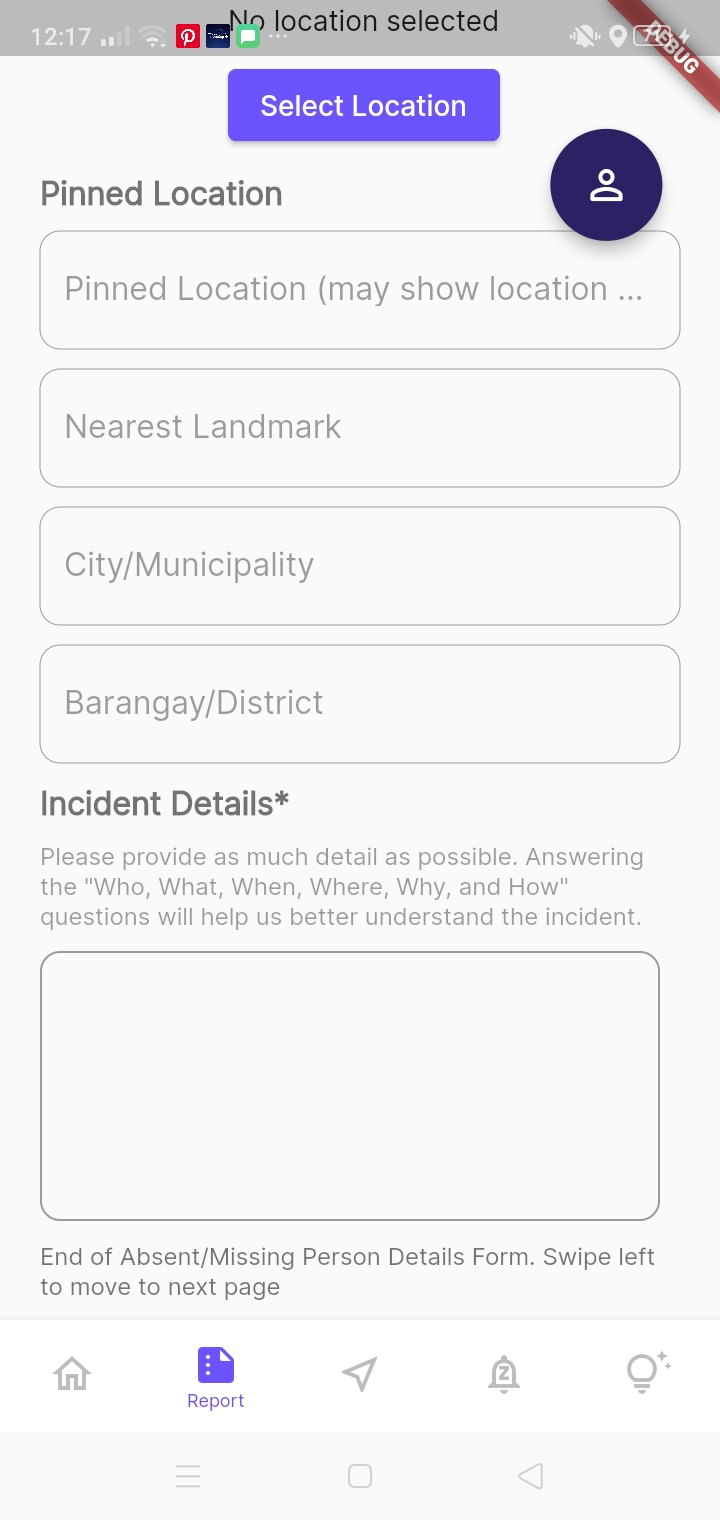
\includegraphics[scale=0.15]{figures/Chapter4/Main/p5-2.jpg}
    \end{subfigure}
    \centering
    \begin{subfigure}[c]{0.30\linewidth}
        \centering
        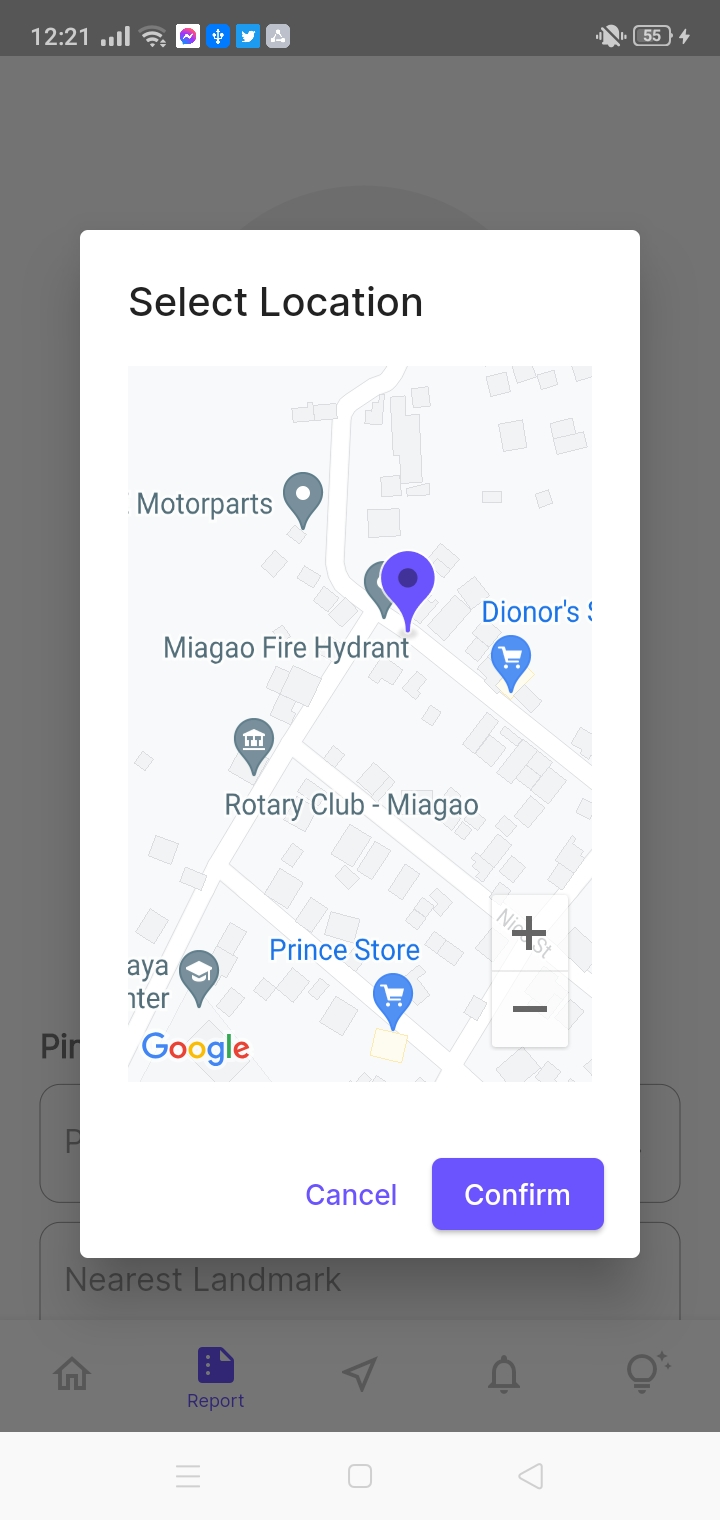
\includegraphics[scale=0.15]{figures/Chapter4/Main/p5-3.jpg}
    \end{subfigure}
    \caption{Report Form Page 5}
    \label{fig:ReportPage5}
\end{figure}

The page requires information such as the report date, which is filled in as the current date, the last seen date, where users will be asked to select the date in a calendar when the missing person was last seen, the last seen location, where the users will be prompted to pin the location the missing person was last seen in a dialog that displays a map centered at the current location of the reportee, and the incident details, where users can input further details they deem as necessary in order to aide in the finding of the missing person. 

\subsubsection{Report Page 6: Confirmation and Authorization}

The sixth, and the last page, as seen in figure \ref{fig:ReportPage6} asks for the confirmation and authorization of the user to finally submit the report that they have filled out. The page would require the signature of the reportee on the signature pad provided citing that, by signing the report, they agree to have the information submitted published and adhere to the rules and responsibilities that come with them submitting the report to the PNP interface for verification. After which, the users can then submit the form to PNP.

\begin{figure}[!h]
    \centering
    \begin{subfigure}[c]{0.40\linewidth}
        \centering
        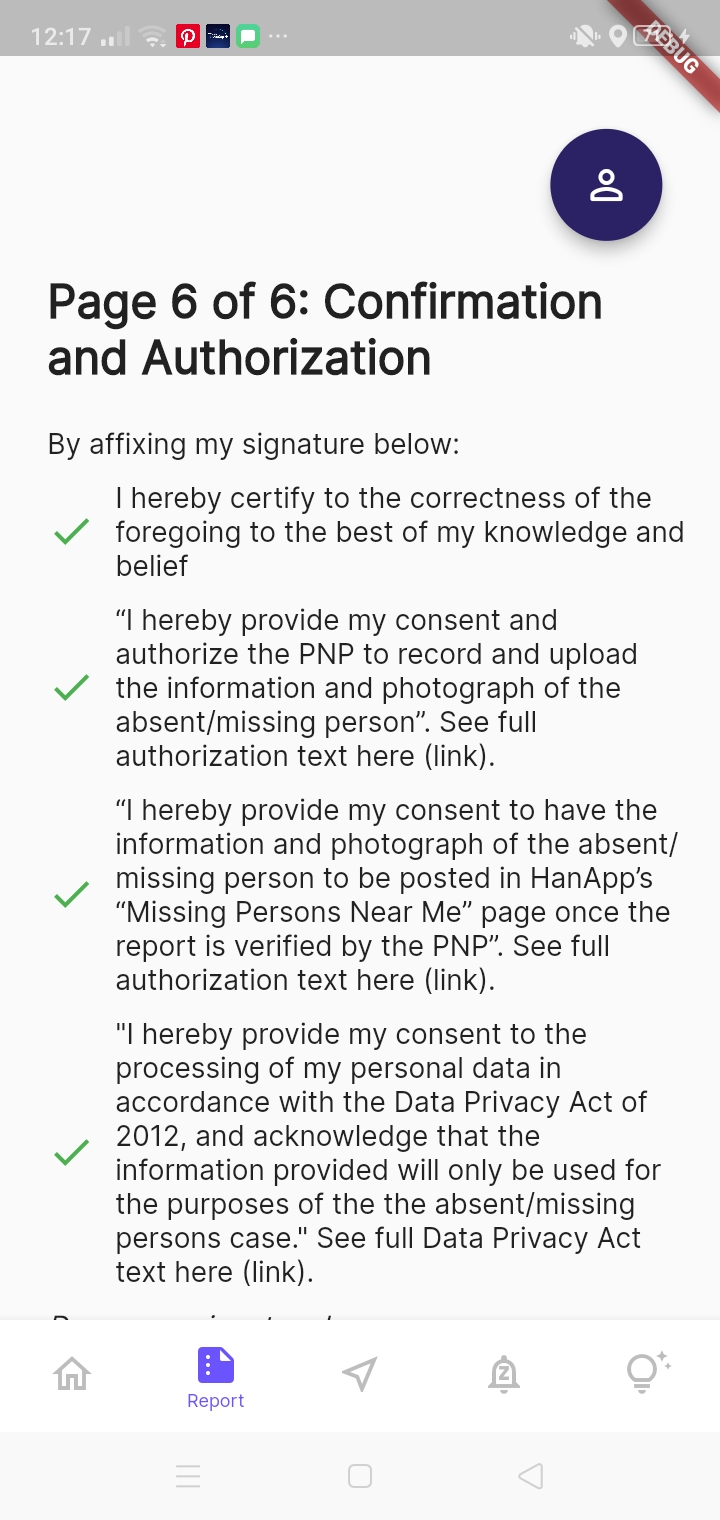
\includegraphics[scale=0.15]{figures/Chapter4/Main/p6-1.jpg}
    \end{subfigure}
    \centering
    \begin{subfigure}[c]{0.40\linewidth}
        \centering
        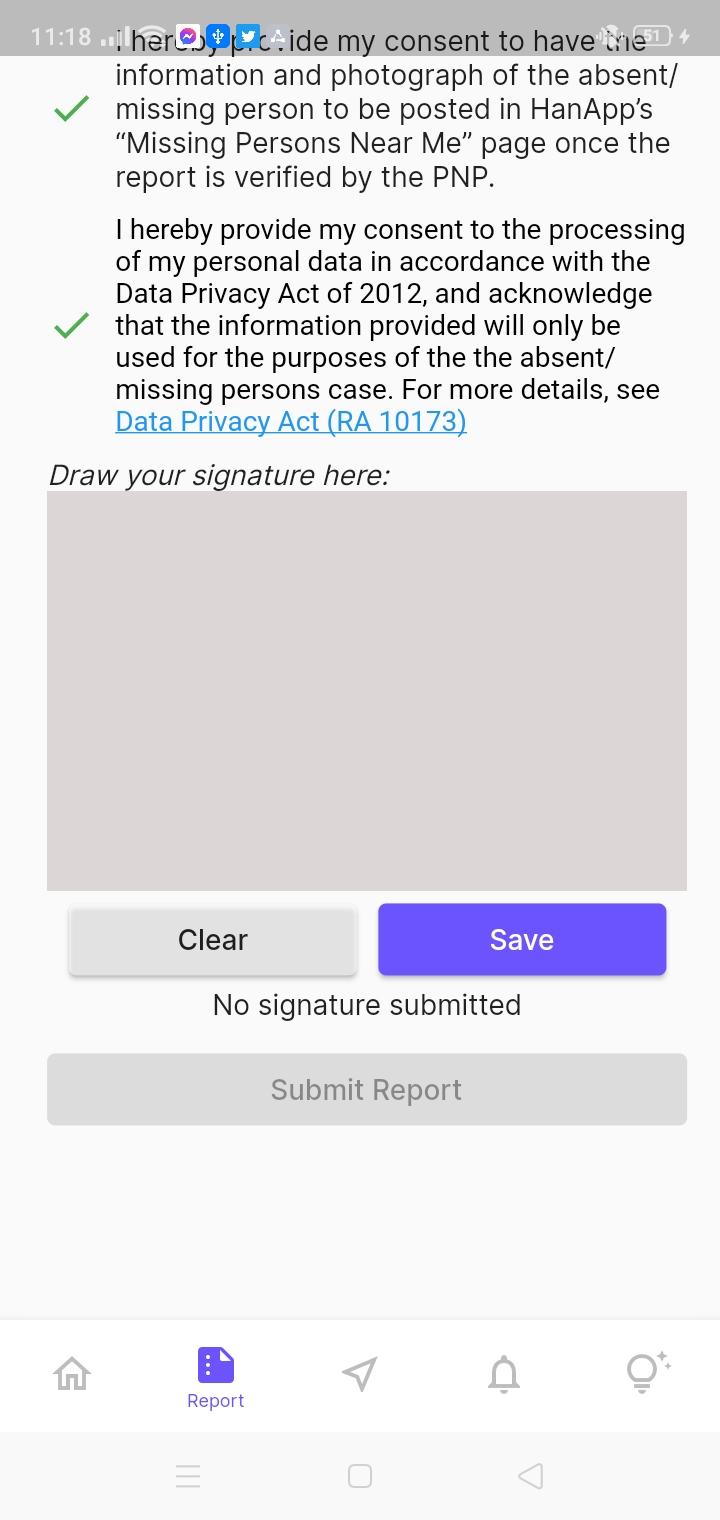
\includegraphics[scale=0.15]{figures/Chapter4/Main/p6-2.jpg}
    \end{subfigure}
    \caption{Report Form Page 6}
    \label{fig:ReportPage6}
\end{figure}

\subsubsection{Report Page Feature: ``Save Report as Draft"}
Upon leaving the report page, by switching to a different page in the main user application, the user is prompted with the options to either discard their report or save it as a draft. If ``Save Draft" is chosen, the user will be shown a confirmation snackbar informing them that the draft of their report has been saved. When the user returns to the report pages with an existing draft page, they will also be shown a snackbar informing them that they are continuing an existing report. These are shown in Figure \ref{fig:saveDraft}.

With this feature, the user will be able to fill out the report at their own pace and convenience. This drastically improves the user (reportee) experience, especially when compared to in-person reporting where they are required to submit all the required information upon filing.
\begin{figure}[!h]
    \centering
    \begin{subfigure}[c]{0.30\linewidth}
        \centering
        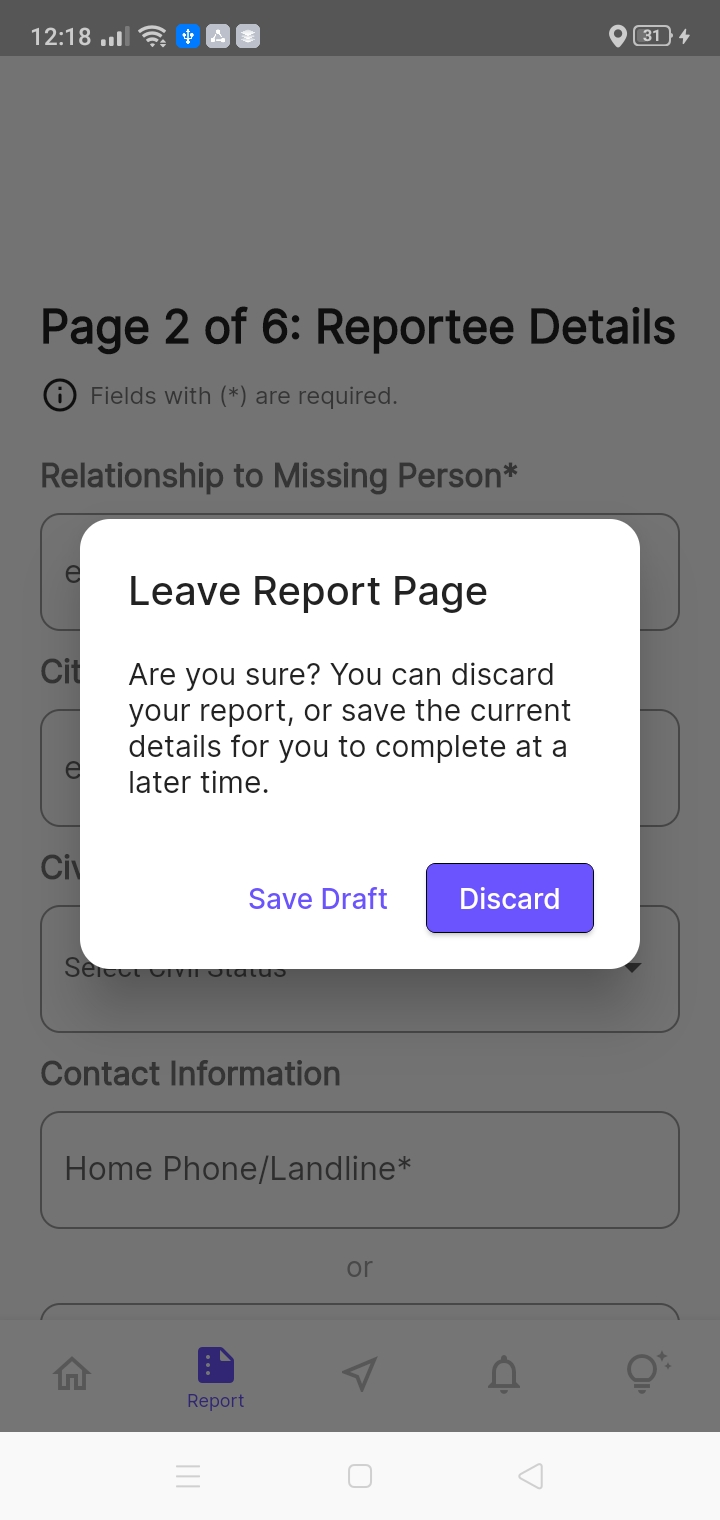
\includegraphics[scale=0.15]{figures/Chapter4/Main/leaveDialog.jpg}
    \end{subfigure}
    \centering
    \begin{subfigure}[c]{0.30\linewidth}
        \centering
        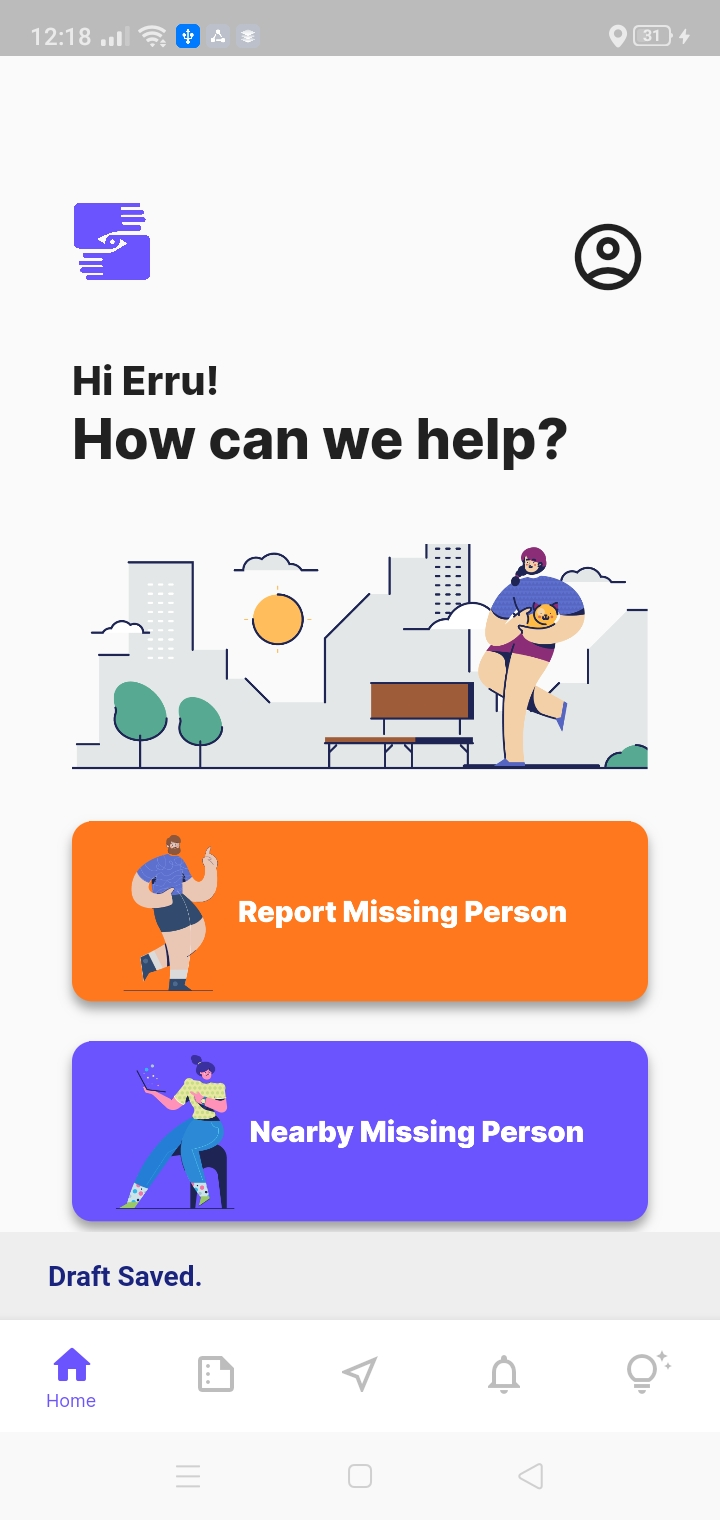
\includegraphics[scale=0.15]{figures/Chapter4/Main/draftSaved.jpg}
    \end{subfigure}
    \centering
    \begin{subfigure}[c]{0.30\linewidth}
        \centering
        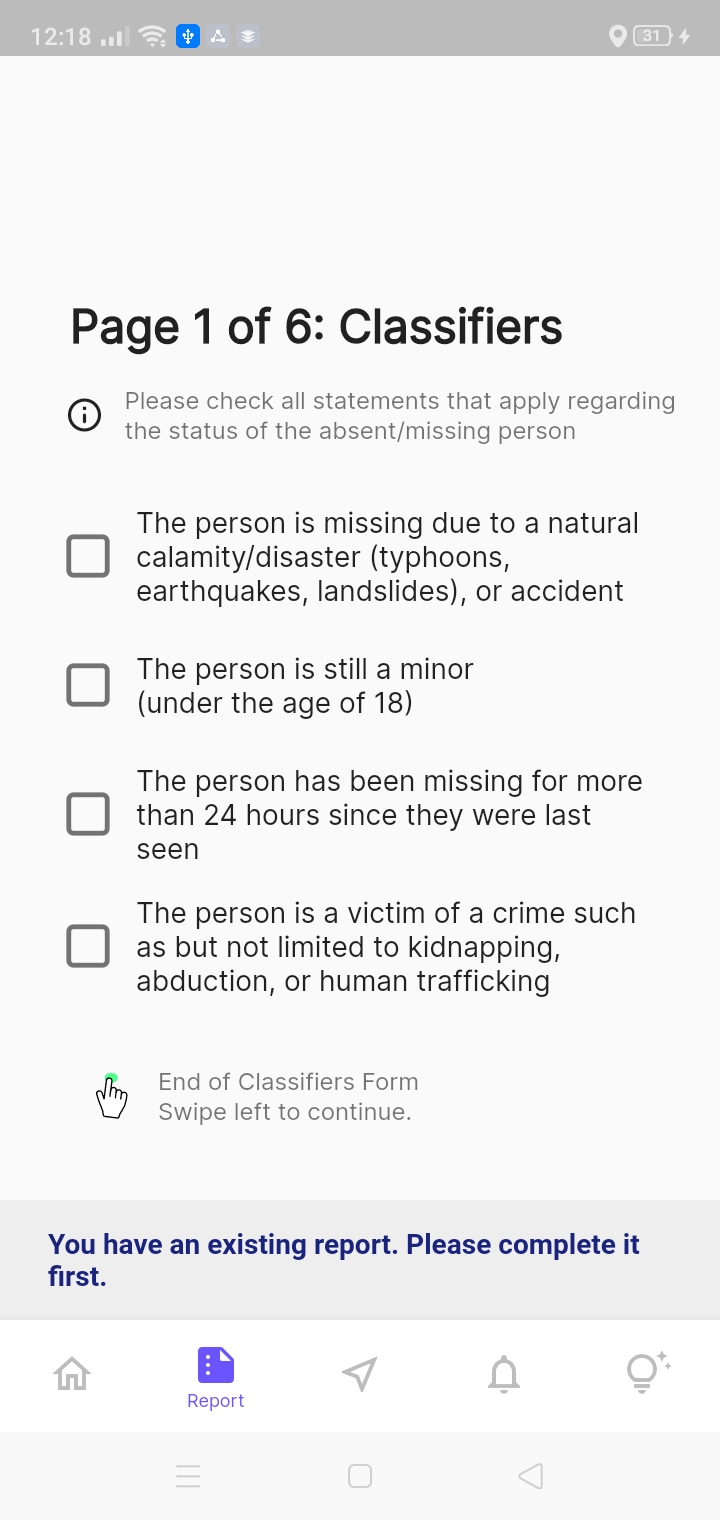
\includegraphics[scale=0.15]{figures/Chapter4/Main/existingReport.jpg}
    \end{subfigure}
    \caption{Save Report As Draft}
    \label{fig:saveDraft}
\end{figure}

\subsection{Nearby Page}

Figure \ref{fig:userTracking} is the interface of tracking missing persons near the user. A location marker will guide the current or last seen whereabouts of a missing person. Only the verified reports that was identified by the PNP through their reports management suite will only be shown. This will allow reports to be validated thoroughly on their end. Apart from that, the user has the liberty to navigate the map, may it be street view or city-wide view by pinching the screen. Also, users can zoom in and zoom out depending on their preference. Landmarks and familiar streets will be shown to guide the users easily on the whereabouts of the missing person. Considering, for example, that a 5-km radius will be visible, it will then encircle the last place the MP was seen.

\begin{figure}[!h]
    \centering
    \begin{subfigure}[c]{0.40\linewidth}
        \centering
        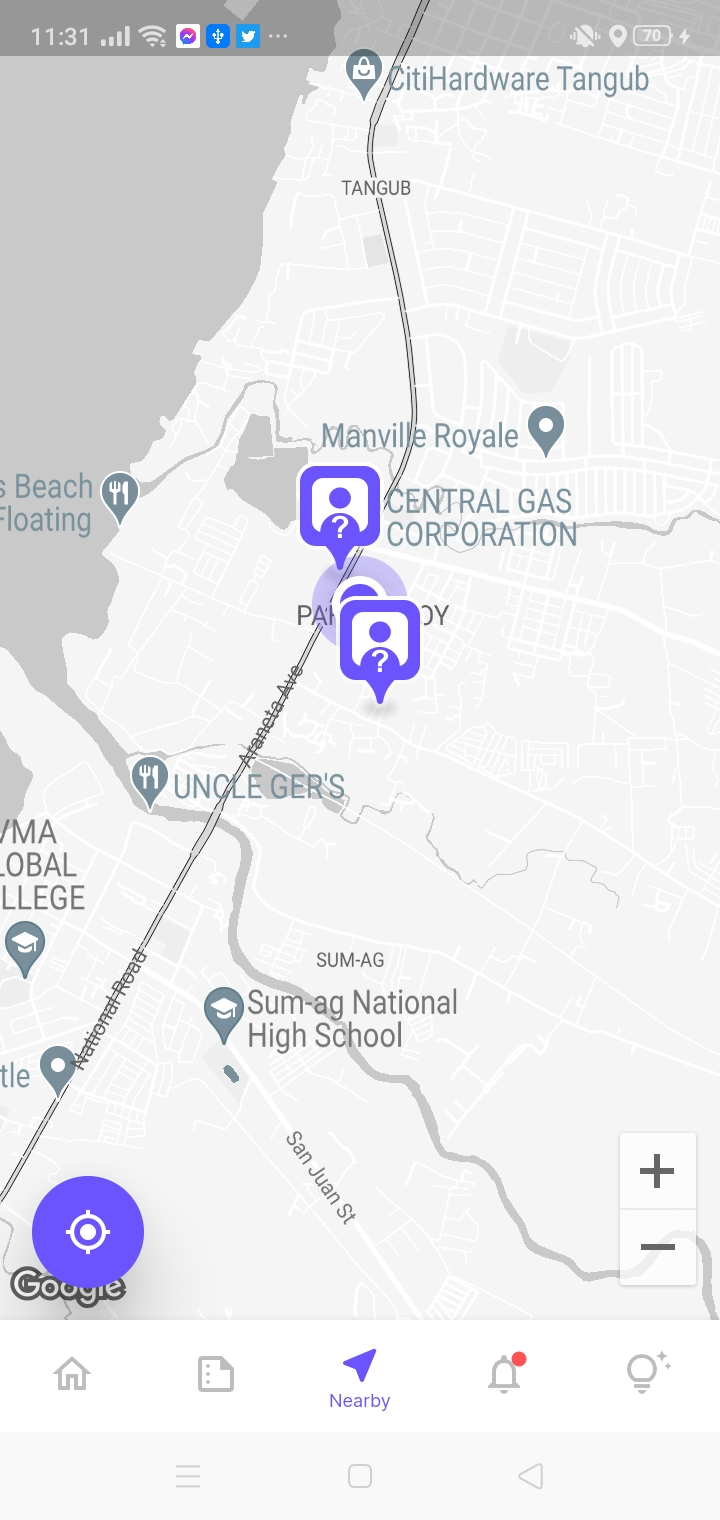
\includegraphics[scale=0.15]{figures/Chapter4/Main/Nearby-1.jpg}
    \end{subfigure}
    \centering
    \begin{subfigure}[c]{0.40\linewidth}
        \centering
        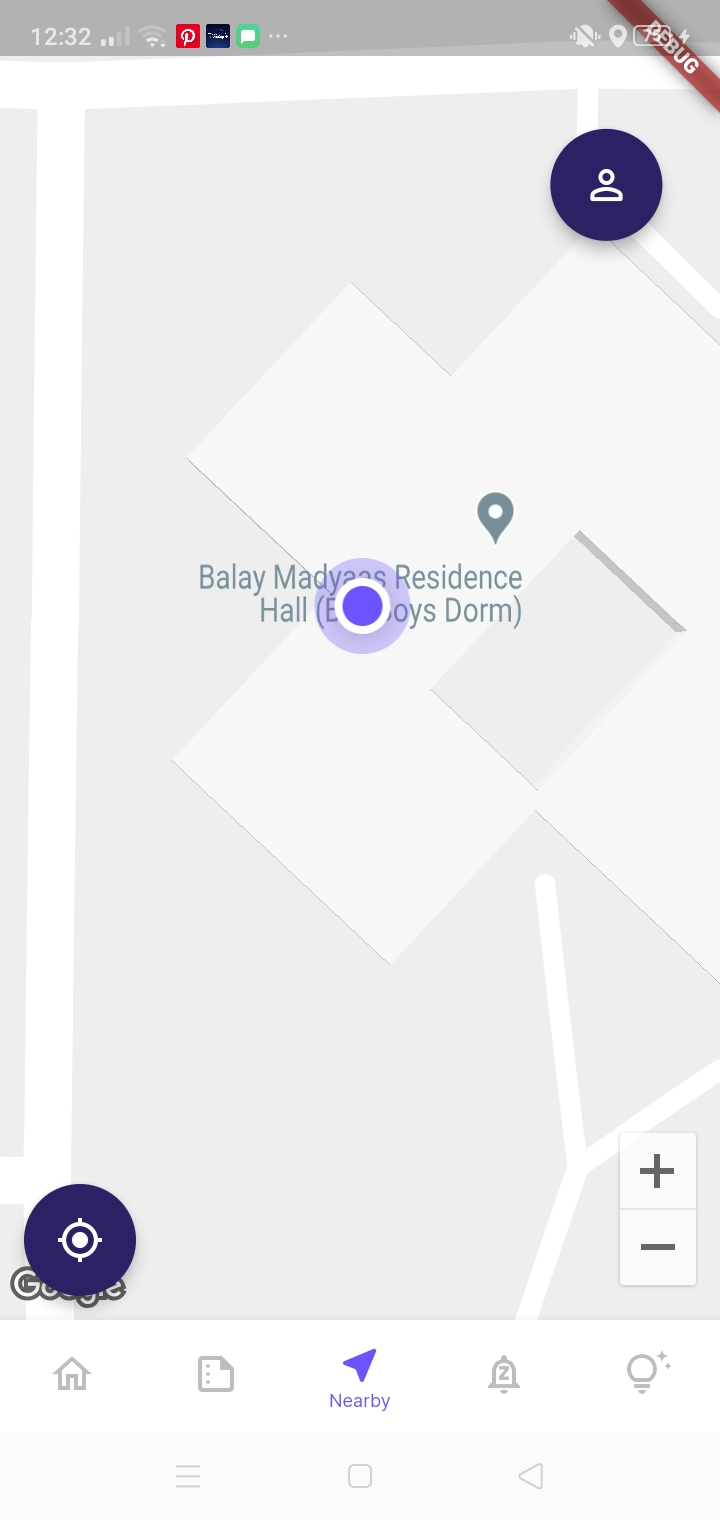
\includegraphics[scale=0.15]{figures/Chapter4/Main/Nearby-2.jpg}
    \end{subfigure}
    \caption{Missing Persons and User Location in Nearby}
    \label{fig:userTracking}
\end{figure}

Another thing that the application also wants to note is how the user can tap on the MPs icon to see the details of descriptions pertaining to the individual. Importantly, there is an additional feature that permits the user to find the nearest route going to the last seen location of the missing person by clicking the 'right turn' icon that will redirect them to Google Maps app, given that they have it on their phone installed. Through all of this, it will enable a swift identification of the person and give the authorities a leeway to make necessary course of action to find these reported missing persons.

\begin{figure}[!h]
    \centering
    \begin{subfigure}[c]{0.30\linewidth}
        \centering
        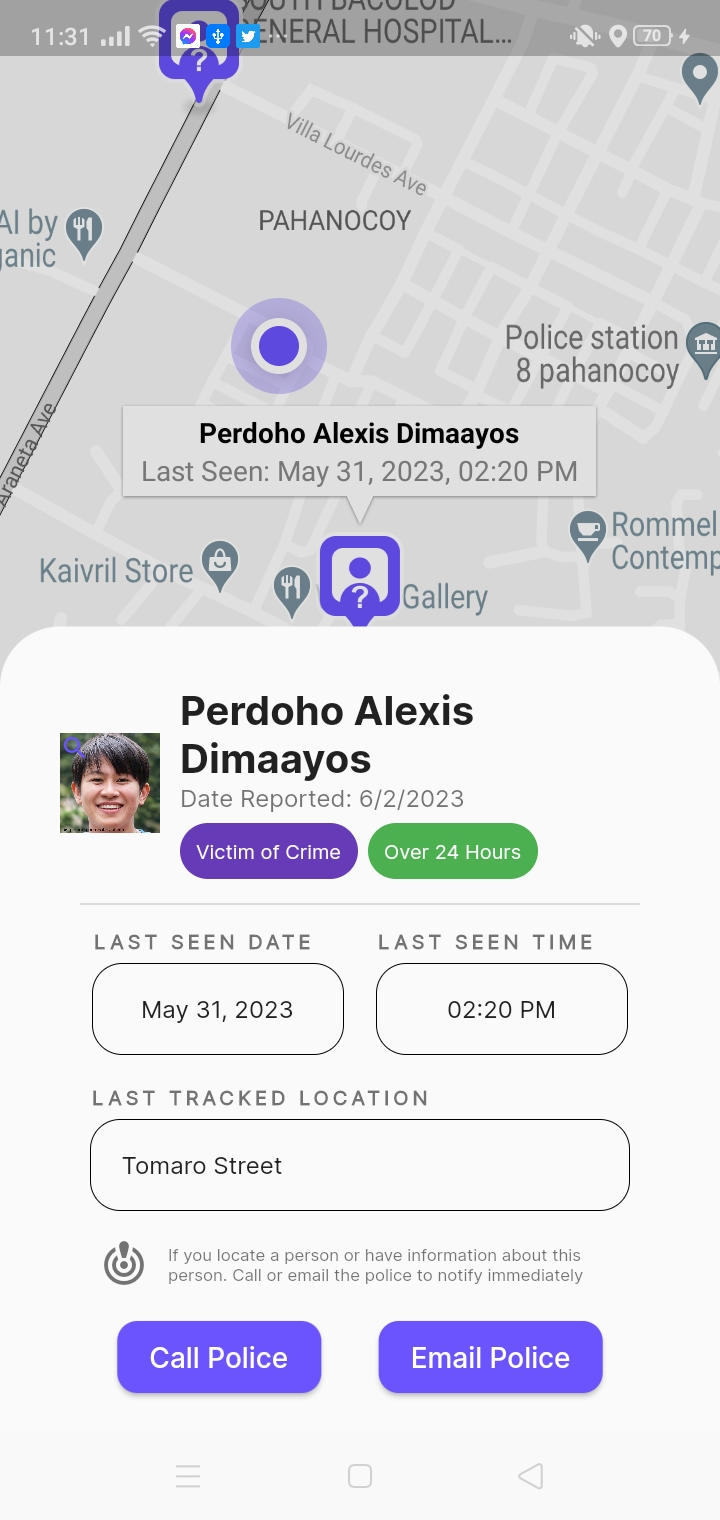
\includegraphics[scale=0.15]{figures/Chapter4/Main/NearbyMP-1.jpg}
    \end{subfigure}
    \centering
    \begin{subfigure}[c]{0.30\linewidth}
        \centering
        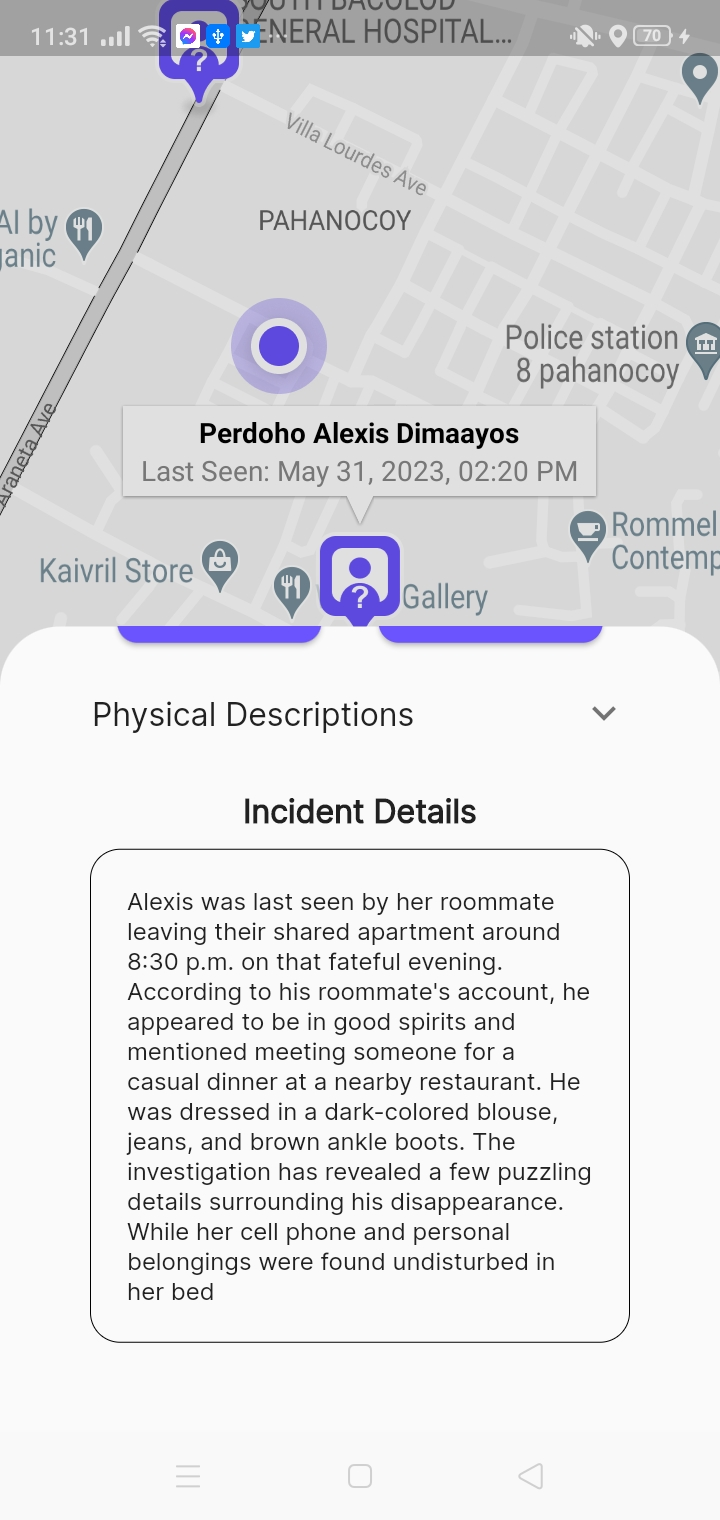
\includegraphics[scale=0.15]{figures/Chapter4/Main/NearbyMP-2.jpg}
    \end{subfigure}
    \centering
    \begin{subfigure}[c]{0.30\linewidth}
        \centering
        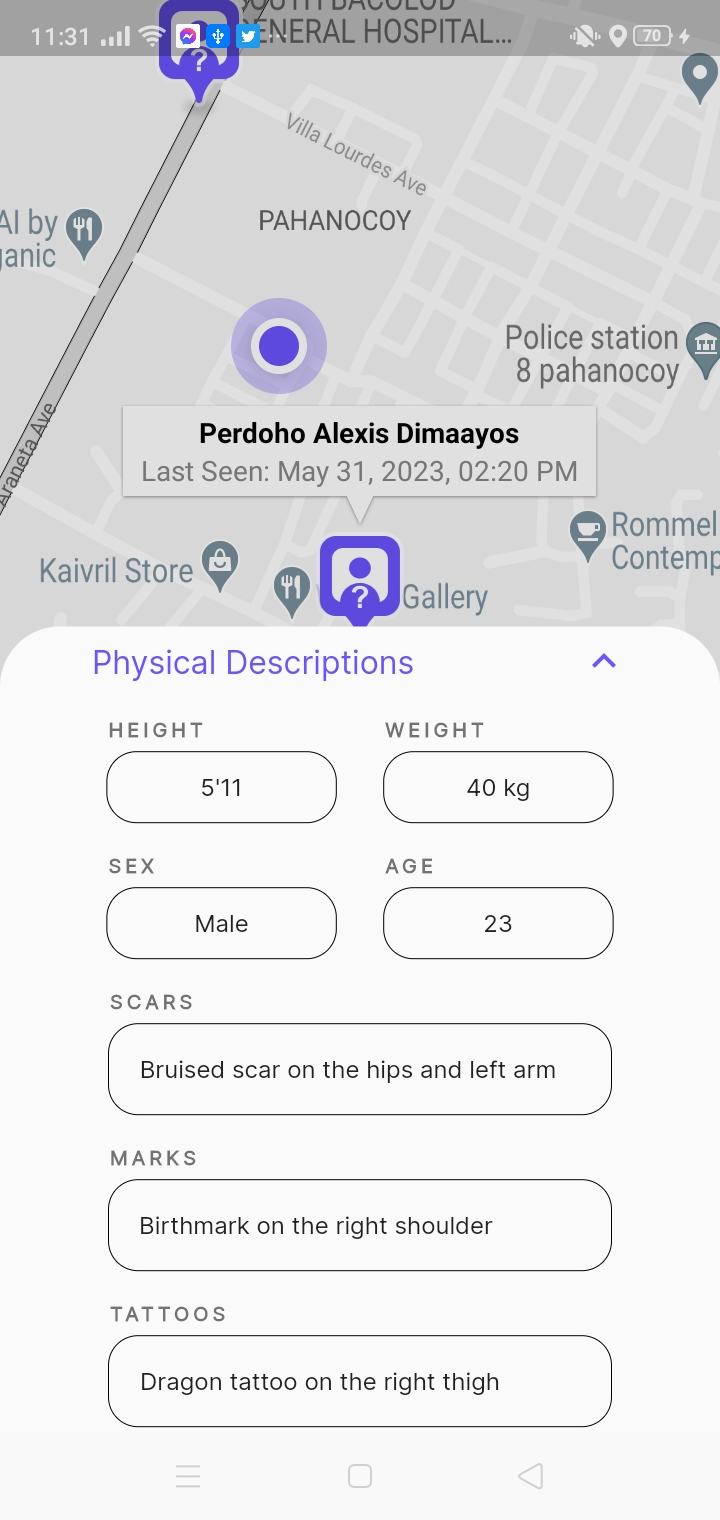
\includegraphics[scale=0.15]{figures/Chapter4/Main/NearbyMP-3.jpg}
    \end{subfigure}
    \caption{Missing Person Details in Nearby}
    \label{fig:notifications}
\end{figure}

\subsection{Notifications Page}

Figure \ref{fig:notifications} illustrates the verified reports by the PNP as shown in \ref{fig:NavRail}. This would allow an easy access to information regarding the missing person in real-time. Not only that, but the user will be alerted by a missing person through the notifications icon red dot in the bottom navigation bar. The each notification will be redirected to the nearby page which gives the user the missing persons' vicinity of their last seen location in the maps.  

\begin{figure}[!h]
    \centering
    \begin{subfigure}[c]{0.30\linewidth}
        \centering
        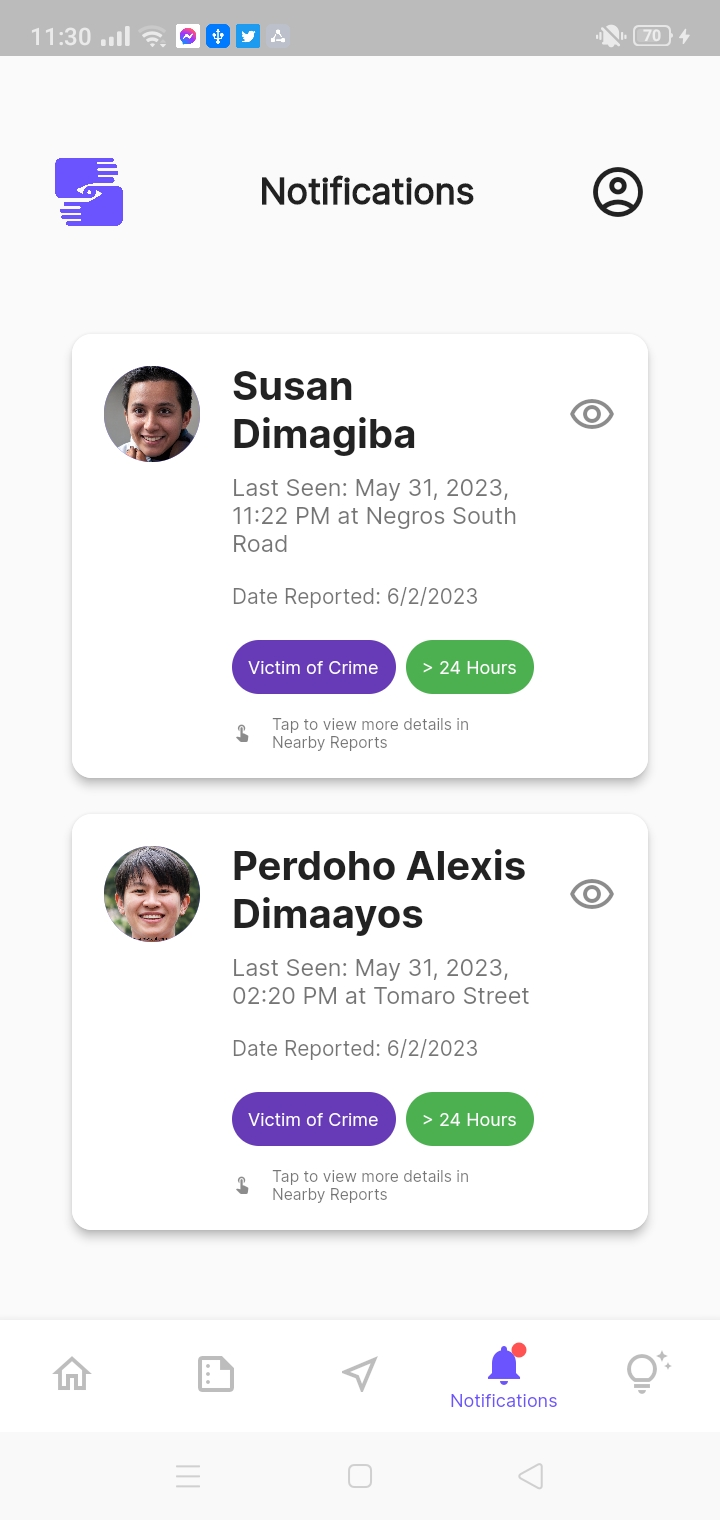
\includegraphics[scale=0.15]{figures/Chapter4/Main/Notifications-1.jpg}
    \end{subfigure}
    \centering
    \begin{subfigure}[c]{0.30\linewidth}
        \centering
        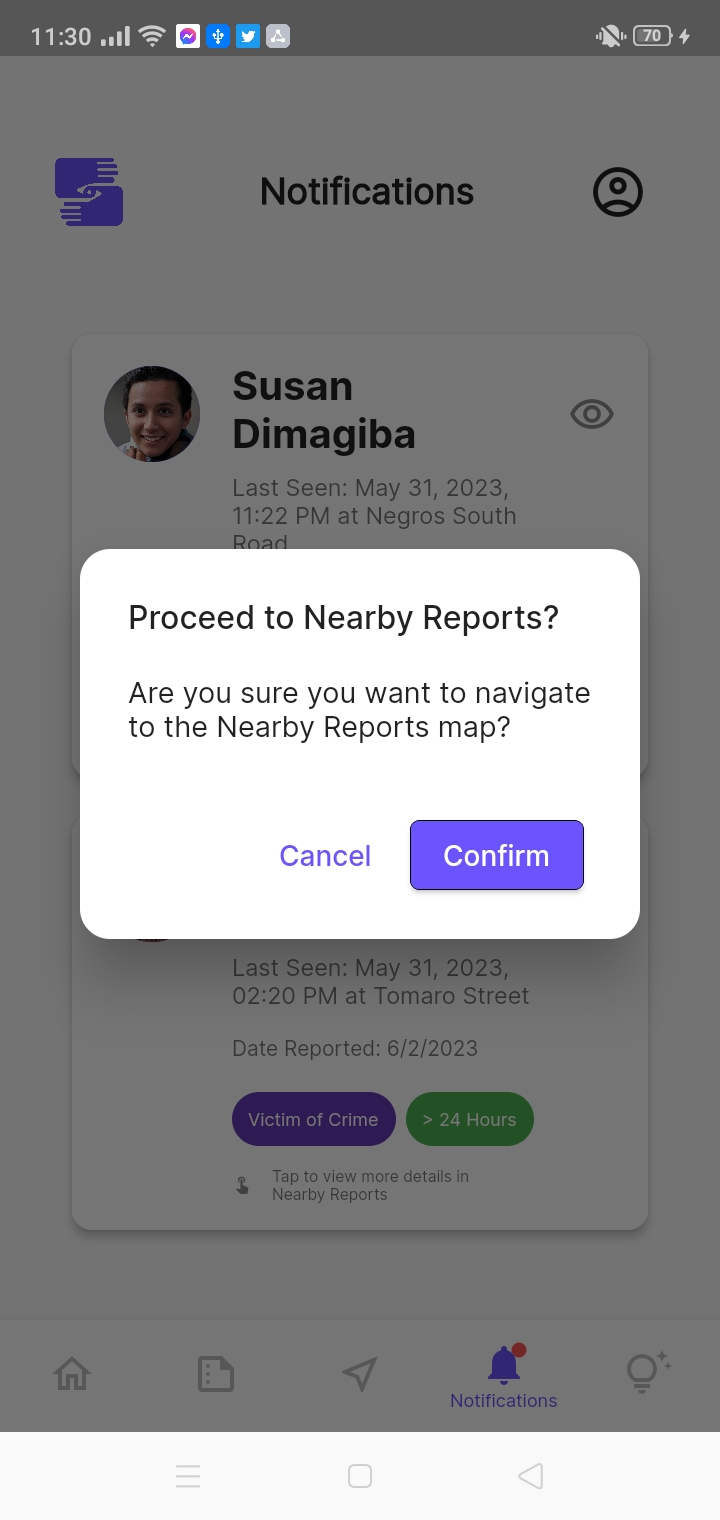
\includegraphics[scale=0.15]{figures/Chapter4/Main/Notifications-2.jpg}
    \end{subfigure}
    \centering
    \begin{subfigure}[c]{0.30\linewidth}
        \centering
        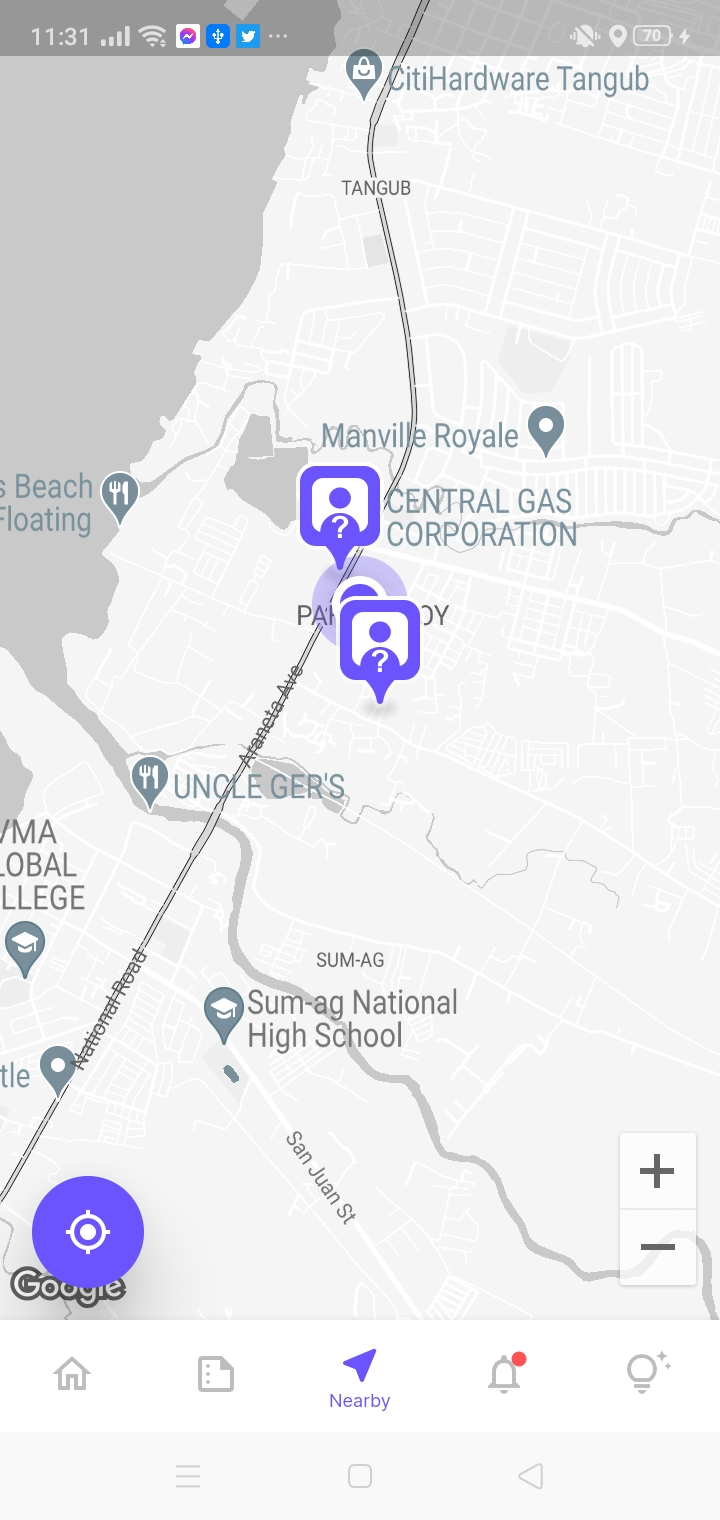
\includegraphics[scale=0.15]{figures/Chapter4/Main/Nearby-1.jpg}
    \end{subfigure}
    \caption{Navigating Notifications Page to Nearby}
    \label{fig:notifications}
\end{figure}

\subsection{Updates Page}

Figure \ref{fig:userReportStatus} demonstrates how the user can visibly see the status of their reported missing persons through the Updates section. For instance, when the user submits their report, the PNP has the liberty to change the status of their report given the information that was forwarded to them as shown in Figure \ref{fig:PNP2}. Not only that, but they will also inspect and verify these as it is sensitive and crucial at this point to confirm whether it needs urgent attention or not (reports with incomplete details would be a factor here). The update of the status is real-time, so when the PNP change its status to a different one, it will automatically change in the user side. The update tags of the reports will consist of four (4) statuses to choose from, namely, Received, Verified, Rejected, or Found. All of these are directly shown to the Updates section of the user's account.

\begin{figure}[!h]
    \centering
    \begin{subfigure}[c]{0.20\linewidth}
        \centering
        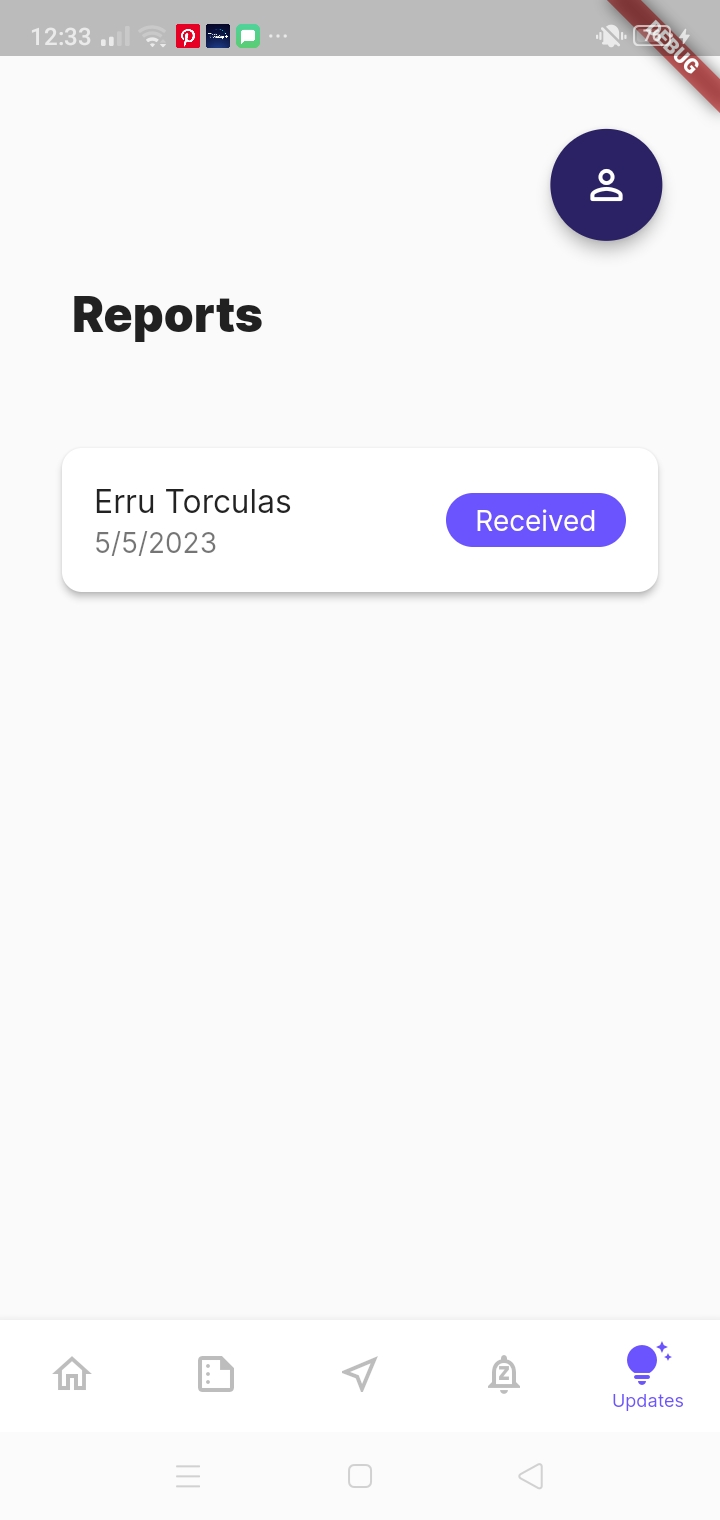
\includegraphics[scale=0.10]{figures/Chapter4/Main/Report-1.jpg}
        \caption{Received}
        \label{fig:StatusReceived}
    \end{subfigure}
    \centering
    \begin{subfigure}[c]{0.20\linewidth}
        \centering
        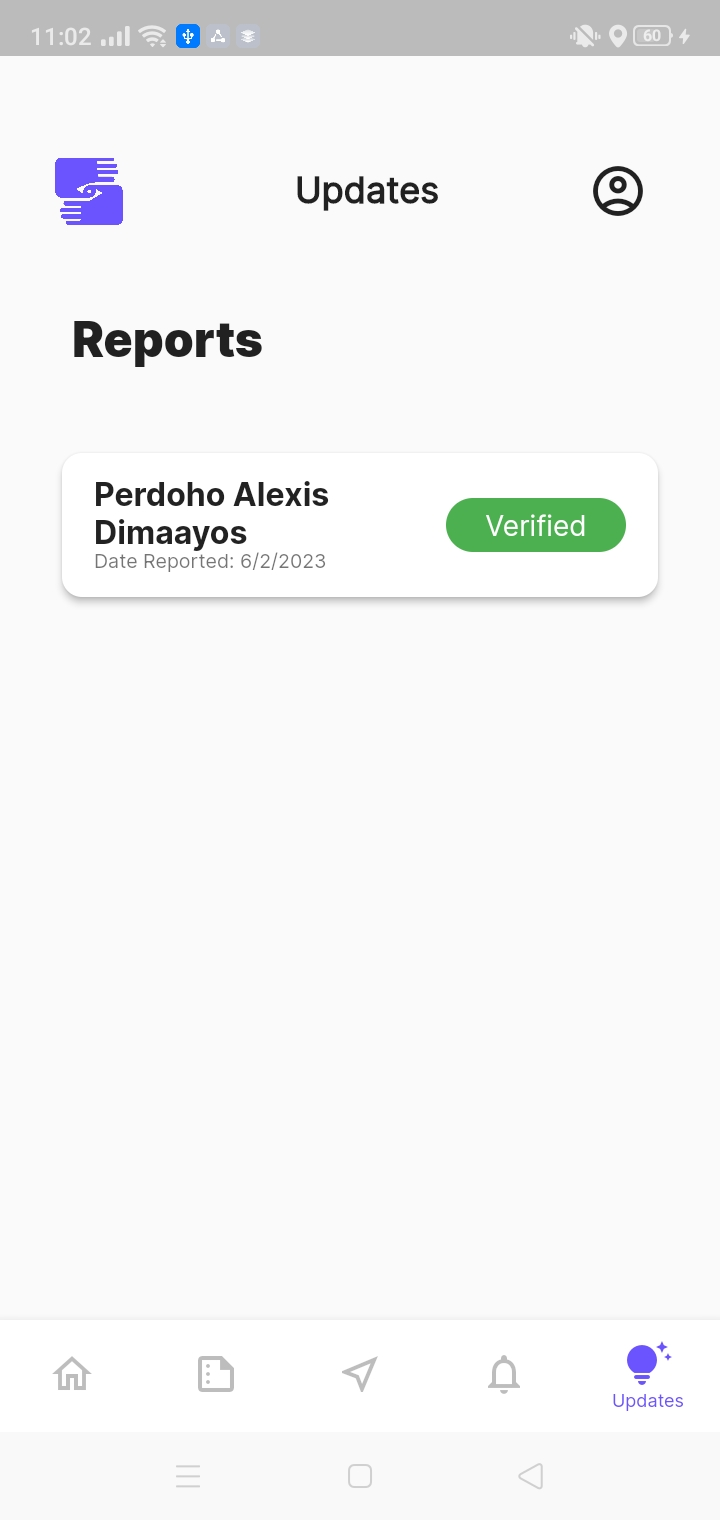
\includegraphics[scale=0.10]{figures/Chapter4/Main/Report-2.jpg}
        \caption{Verified}
        \label{fig:StatusVerified}
    \end{subfigure}
    \centering
    \begin{subfigure}[c]{0.20\linewidth}
        \centering
        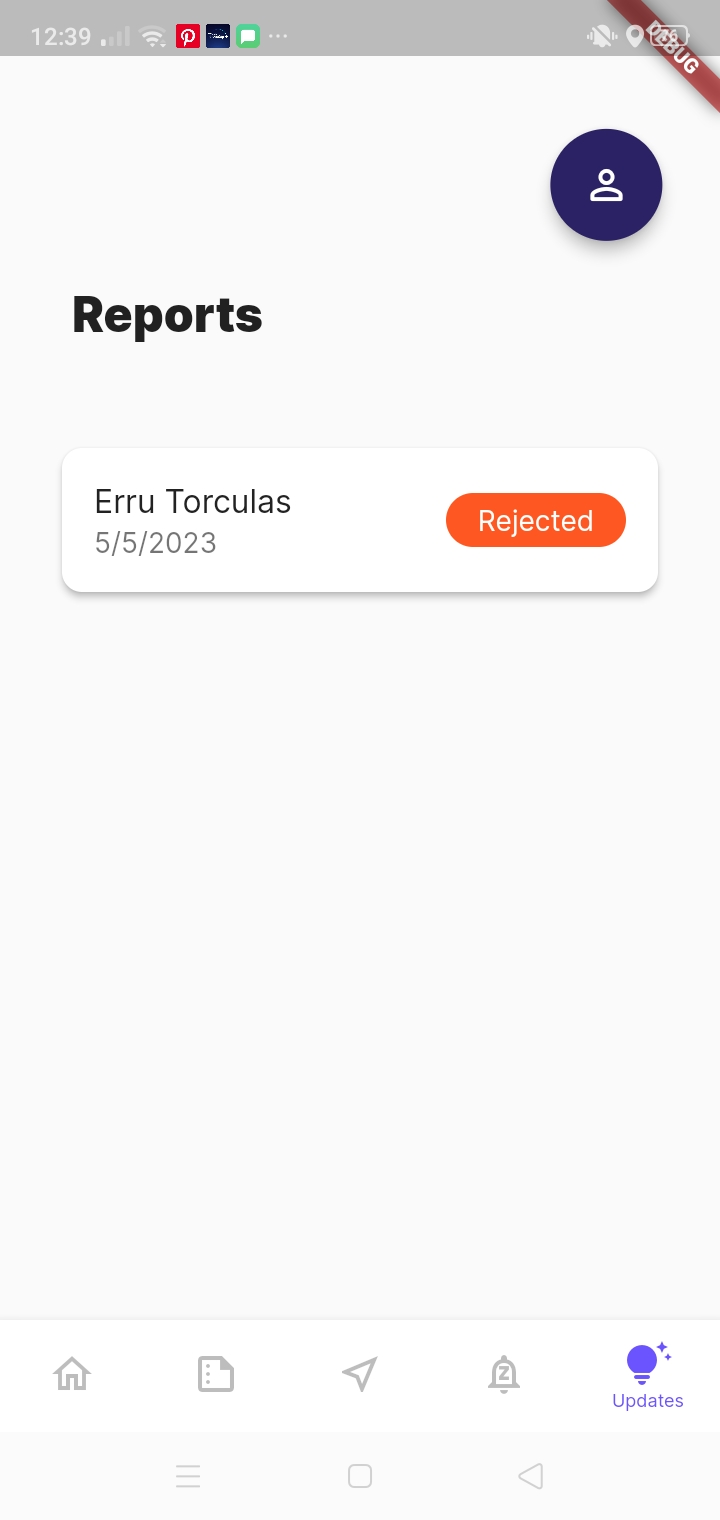
\includegraphics[scale=0.10]{figures/Chapter4/Main/Report-3.jpg}
        \caption{Rejected}
        \label{fig:StatusRejected}
    \end{subfigure}
        \centering
    \begin{subfigure}[c]{0.20\linewidth}
        \centering
        \includegraphics[scale=0.10]{figures/Chapter4/Main/Report-4.jpg}
        \caption{Found}
        \label{fig:StatusFound}
    \end{subfigure}
    \caption{Updates Page with Status of Report}
    \label{fig:userReportStatus}
\end{figure}

\section{UI/UX Design Implementation}

\subsection{Application Suite Logo}

The HanApp logo, as seen in Figure \ref{fig:hanappLogo}, is an indigo-colored logo of two horizontally-oriented hands whose thumbs meet in between and form an ``eye", and with the fingers forming ``speed lines". The two hands in the logo have various meanings: (1) connecting the PNP and the reporter, (2) connecting the reporter to the general community, and (3) the missing person reuniting with the reporter, whereas the eye in the middle imply that the application is about looking for missing persons. Moreover, the ``speed lines" formed by the fingers help imply that the application makes the process of reporting, verifying, disseminating, and resolving missing persons cases faster. 

As such, HanApp logo meets the application logo requirement such that it is distinct, meaningful, and cohesive with the HanApp's UI/UX design and color theme.
\begin{figure}[!h]
    \centering
    \begin{minipage}[c]{0.50\linewidth}
        \centering
        \includegraphics[scale=0.15]{figures/hanappLogo.png}
        \caption{HanApp Application Logo}
        \label{fig:hanappLogo}
    \end{minipage}
\end{figure}

\subsection{UI/UX Design}

As shown in the preceding sections, the UI/UX design of the application suite were able to meet the UI/UX Design requirements listed in the previous chapter, namely:

\begin{enumerate}
    \item The application's frontend design ensures accessibility and ease of use in its choice of font size and family, layout, and colors.
    \item The English language is utilized throughout the entire application with no grammatical errors and with the use of simple and straightforward wordings.
    \item The report form pages were simplified and incorporated the use of checkboxes, radio buttons, buttons for save/upload prompts, and text fields as well as validators, ensuring not only ease of use but also the completeness and correctness in the submitted reports. 
\end{enumerate}

\section{Backend Framework - Firebase}

Firebase handles both account management and data management. As such, the following sections will discuss and show the backend framework at which user accounts and reports data is stored and managed.

\subsection{User Accounts Authentication and Storage}

As seen in Figure \ref{fig:firebaseAuth}, user accounts are stored in Firebase's Authentication page. It shows the user account's unique UID, email, date created, and last signed in page. Firebase also handles the authentication service which was shown in the user account authentication section above.
\begin{figure}[!h]
    \centering
    \begin{minipage}[c]{1\linewidth}
        \centering
        \includegraphics[scale=0.25]{figures/Chapter4/Firebase/authentication.png}
        \caption{Authentication Database}
        \label{fig:firebaseAuth}
    \end{minipage}
\end{figure}
\subsection{Realtime Database (RTDB) for User Data and Reports}

All user data (for main and PNP accounts) and their reports are stored in the RTDB as seen in Figure \ref{fig:firebaseRTDB}. There are three main ``nodes" storing the Main Users user data, PNP Accounts user data, and Reports data. The Reports node stores and organizes all reports that have been submitted through the application under each user.
\begin{figure}[!h]
    \centering
    \begin{minipage}[c]{1\linewidth}
        \centering
        \includegraphics[scale=0.25]{figures/Chapter4/Firebase/rtdbReports.png}
        \caption{Realtime Database User Data and Reports}
        \label{fig:firebaseRTDB}
    \end{minipage}
\end{figure}
\subsubsection{Firebase Storage for Images Submitted in Reports}

Figure \ref{fig:firebaseStorage} contains all the images submitted in the reports including the reportee's signature. As seen in the header address line, images are organized under a ``Reports" node, under each ``User" node, and under each ``Report Number" node. This setup allows for a more organized way of storing images submitted for easier retrieval.
\begin{figure}[!h]
    \centering
    \begin{minipage}[c]{1\linewidth}
        \centering
        \includegraphics[scale=0.25]{figures/Chapter4/Firebase/storage.png}
        \caption{Firebase Storage}
        \label{fig:firebaseStorage}
    \end{minipage}
\end{figure}
\section{Data Privacy and Security Measures}

\subsection{Password Security}

As seen in Figure \ref{fig:passwordHash}, in the Firebase Authentication Console, the password for each user is not displayed, only their email (as Identifier), the account the date was created and last signed in, and their unique Firebase UID. 

Moreover, Firebase Authentication uses hash scripts to encrypt password to avoid encrypted password data from being used even when spoofed in unsafe networks.

\begin{figure}[!h]
    \centering
    \begin{minipage}[c]{1\linewidth}
        \centering
        \includegraphics[scale=0.25]{figures/Chapter4/Firebase/passwordHash.png}
        \caption{Firebase Storage}
        \label{fig:passwordHash}
    \end{minipage}
\end{figure}

\subsection{Data Privacy, Collection, and Usage}

\subsubsection{Data Scope}

To limit data privacy issues, the HanApp application suite only collects and stores information from users that pertain to account management (signing up, logging in), and reporting (reportee, absent/missing person, and incident information) and dissemination of missing persons cases. Furthermore, all the data required in the missing persons report form are the same information required by the PNP guidelines on missing persons cases, except for the reportee ID and selfie photograph which were included in lieu of  reporting and presenting their ID in-person.

\subsubsection{User Agreements on Report Data}

Prior to submitting a missing persons report, users are informed that by affixing their signature to the report, they:
\begin{itemize}
    \item Certify to the correctness of information being submitted
    \item Consent and authorize the PNP to record and upload the information and photograph (most recent photo of the absent/missing person) to the Missing Person Website
    \item Consent to have the aforementioned information posted in HanApp's ``Nearby Missing Persons" page once the report is verified by the PNP
    \item Consent to the processing of their personal data in accordance with the Data Privacy Act of 2012, and acknowledge that their information will only be used for the purposes of the absent/missing persons case.
\end{itemize}

This is shown in the Confirmation and Authorization page of the Report Form, as seen in Figure \ref{fig:ReportPage6}. The users are also provided a link to official government websites containing the PNP Memorandum Circular 2016-033 and the Data Privacy Act of 2012 for their perusal.


\subsubsection{Location Data Usage and Anonymity}

The only location data being stored are the last seen location of the absent/missing person as they are required for the verification and dissemination of reports. Users' current location data will be read by the application for the purpose of location-based notifications for PNP-verified missing persons reports near the user's location. However, this data is not collected or stored in the HanApp's backend database. 


\section{Limitations and Issues}

This section discusses the technological and resource limitations and issues encountered during the application suite’s development, testing, and implementation. It is crucial to note that, while these do not hinder the application suite from working nor prevent it from meeting its requirements, they do have an impact on the quality of service provided by HanApp's system prototype. 

\subsection{Geocoding Limitations}

This is with regards to the Report form’s “last known location selector” in the main user application. As shown earlier, the user is prompted to select the last known location by pinning it on a map, this then retrieves the latitude and longitude of the pinned location. The Flutter geocoding package is then used to handle the Google Geocoding API to retrieve information from Google Maps in order to perform reverse geocoding which is the process of fetching the address based on the latitude and longitude provided. 

The main issue with this is that the address retrieved from geocoding may sometimes be incomplete or inaccurate. For example, the geocoding API retrieves “locality” and “sublocality” information. While the locality, which should be the city or town address, is retrieved accurately, the sublocality, which should be the barangay, returns either the barangay or the district depending on what is registered as “sublocality” for that location. Additionally, the sublocality may not be registered in some circumstances and no barangay/district address is returned. 

Although this issue is circumvented through the use of location snapshots (a snapshot of the pinned location in Google Maps) which allow both the PNP and users who are able to view PNP-verified reports to determine the barangay or district from the snapshot, it does affect the last known location address written on the report.

\subsection{PNP Resources and Data Limitations}

\subsubsection{Absence of PNP Station Directory}

There is currently no comprehensive national directory that lists every police station in the country. Because of this, the address and contact information of every station must be manually searched and entered into a database. As a result, each police station’s HanApp account had its location and contact information hard-coded for testing purposes.

\subsubsection{\textbf{Absence of PNP Precinct Map Data}}

The PNP station in charge incidents is based on the location of the incident. In missing persons cases, the case should be reported to and is handled by a certain police station if the last known location of the absent/missing person is within its precinct (or area of jurisdiction). As such, the report routing through HanApp should also forward missing persons reports to the police station in whose jurisdiction covers the selected last known location. The problem is that there is no PNP station precinct map data.

In the absence of precinct map data, the HanApp system prototype routes the reports to the PNP station account nearest to the selected last known location of the absent/missing person. However, this may sometimes result in misrouting. For example, the last known location of the missing person is closest to the Police Station A than it is to the Police Station B, but the location may actually be within the Police Station B’s precinct or area of jurisdiction.

\newpage
\section{Summary of Results}

To summarize the results of the study, the checklist of application requirements, Table \ref{table:reqChecklist}, as seen in the previous chapter, was updated to show whether all the requirements for HanApp application suite have been met. As seen in Table \ref{table:results_reqChecklist}, all requirements for the application's system prototype were satisfied.
\begin{table}[]
\caption{Requirements Checklist Results}
\label{table:results_reqChecklist}
\begin{tabular}{|lc|}
\hline
\multicolumn{1}{|c|}{\textbf{REQUIREMENTS}}                                                                                                                         & \textbf{\begin{tabular}[c]{@{}c@{}}ACCOMPLISHED\\ (Y/N)\end{tabular}} \\ \hline
\multicolumn{2}{|l|}{\textbf{Backend Requirements}}                                                                                                                                                                                         \\ \hline
\multicolumn{1}{|l|}{Serverless Architecture}                                                                                                                       & Y                                                                     \\ \hline
\multicolumn{1}{|l|}{\begin{tabular}[c]{@{}l@{}}Realtime Database structure \\ for Main User and PNP profiles\end{tabular}}                                         & Y                                                                     \\ \hline
\multicolumn{1}{|l|}{Realtime Database structure for Reports}                                                                                                       & Y                                                                     \\ \hline
\multicolumn{1}{|l|}{Images and other media storage}                                                                                                                & Y                                                                     \\ \hline
\multicolumn{2}{|l|}{\textbf{Privacy Requirements}}                                                                                                                                                                                         \\ \hline
\multicolumn{1}{|l|}{User Password Encryption}                                                                                                                      & Y                                                                     \\ \hline
\multicolumn{1}{|l|}{Data Privacy, Collection, and Usage}                                                                                                           & Y                                                                     \\ \hline
\multicolumn{2}{|l|}{\textbf{User Interface Requirements}}                                                                                                                                                                                  \\ \hline
\multicolumn{1}{|l|}{User (or Main) Interface}                                                                                                                      & Y                                                                     \\ \hline
\multicolumn{1}{|l|}{PNP Admin App Interface}                                                                                                                       & Y                                                                     \\ \hline
\multicolumn{2}{|l|}{\textbf{Functional Requirements}}                                                                                                                                                                                      \\ \hline
\multicolumn{1}{|l|}{User Registration}                                                                                                                             & Y                                                                     \\ \hline
\multicolumn{1}{|l|}{PNP Admin Account Creation}                                                                                                                    & Y                                                                     \\ \hline
\multicolumn{1}{|l|}{Reporting and Receiving Updates}                                                                                                               & Y                                                                     \\ \hline
\multicolumn{1}{|l|}{Save Report as Draft}                                                                                                               & Y                                                                                                \\ \hline

\multicolumn{1}{|l|}{Receive, Manage, and Verify Reports (PNP)}                                                                                                     & Y                                                                     \\ \hline
\multicolumn{1}{|l|}{\begin{tabular}[c]{@{}l@{}}Accessing PNP-Verified Reports and receiving \\ Location-based notification for PNP-verified MP cases\end{tabular}} & Y                                                                     \\ \hline
\multicolumn{2}{|l|}{\textbf{UI/UX Design Requirements}}                                                                                                                                                                                    \\ \hline
\multicolumn{1}{|l|}{Application Icon Design}                                                                                                                       & Y                                                                     \\ \hline
\multicolumn{1}{|l|}{User Interface Design}                                                                                                                         & Y                                                                     \\ \hline
\multicolumn{1}{|l|}{User Experience Design}                                                                                                                        & Y                                                                     \\ \hline
\end{tabular}
\end{table}
For the main user application interface (and its features), the pre-final stable build of the application was alpha tested and were agreed on to meet the requirements. As for the PNP admin application interface, extensive alpha testing by the developers was conducted prior to verifying that the requirements for the PNP admin application interface were satisfied. Overall, despite the limitations and issues encountered, all the requirements and features were met and incorporated into HanApp's system prototype.

               %LaTeX source file for Chapter 4: Results and Discussions
%   Filename    : chapter_5.tex 
\chapter{Conclusion}
This chapter  summarizes your SP and provides conclusions regarding your results and analyses.  Provide recommendations on what ought to be done with your SP or provide further directions on the topic you covered.                %Chapter 5: conclusion and recommendations
%   Filename    : chapter_6.tex 
\chapter*{References}
\markboth{REFERENCES}{REFERENCES}
\bibliographystyle{apacite}       
\bibliography{myreferences}                    %Chapter 6: references



% removed appendix, no content
%\appendix                         %specify appendices
%%%%%%%%%%%%%%%%%%%%%%%%%%%%%%%%%%%%%%%%%%%%%%%%%%%%%%%%%%%%%%%%%%%%%%%%%%%%%%%%%%%%%%%%%%%%%%%%%%%%%%%
%
%   Filename    : appendix_A.tex 
%
%   Description : This file is for including the Research Ethics Documents (delegated as Appendix A) 
%                 
%%%%%%%%%%%%%%%%%%%%%%%%%%%%%%%%%%%%%%%%%%%%%%%%%%%%%%%%%%%%%%%%%%%%%%%%%%%%%%%%%%%%%%%%%%%%%%%%%%%%%%

\chapter{User/Main Interface}
\label{sec:appendixa}

\begin{figure}[!h]
    \centering
    \begin{subfigure}[c]{0.30\linewidth}
        \centering
        \includegraphics[scale=0.15]{figures/Chapter4/Main/PermissionOff.jpg}
    \end{subfigure}
    \centering
    \begin{subfigure}[c]{0.30\linewidth}
        \centering
        \includegraphics[scale=0.15]{figures/Chapter4/Main/b4-Home.jpg}
    \end{subfigure}
    \centering
    \begin{subfigure}[c]{0.30\linewidth}
        \centering
        \includegraphics[scale=0.15]{figures/Chapter4/Main/Home.jpg}
    \end{subfigure}
    \caption{Location Permissions Call-to-action}
    \label{fig:locationPermission}
\end{figure}

\begin{figure}[!h]
    \centering
    \begin{subfigure}[c]{0.30\linewidth}
        \centering
        \includegraphics[scale=0.15]{figures/Chapter4/Main/Nearby-1.jpg}
    \end{subfigure}
    \centering
    \begin{subfigure}[c]{0.30\linewidth}
        \centering
        \includegraphics[scale=0.15]{figures/Chapter4/Main/CallPNP.jpg}
    \end{subfigure}
    \centering
    \begin{subfigure}[c]{0.30\linewidth}
        \centering
        \includegraphics[scale=0.15]{figures/Chapter4/Main/EmailPNP.jpg}
    \end{subfigure}
    \caption{Contact Nearest PNP Station}
    \label{fig:contactPNP}
\end{figure}

\begin{figure}[!h]
    \centering
    \begin{subfigure}[c]{0.40\linewidth}
        \centering
        \includegraphics[scale=0.15]{figures/Chapter4/Main/leaveDialog.jpg}
    \end{subfigure}
    \centering
    \begin{subfigure}[c]{0.40\linewidth}
        \centering
        \includegraphics[scale=0.15]{figures/Chapter4/Main/reportDiscarded.jpg}
    \end{subfigure}
    \caption{Discard Report}
    \label{fig:submitReport}
\end{figure}


\begin{figure}[!h]
    \centering
    \begin{subfigure}[c]{0.40\linewidth}
        \centering
        \includegraphics[scale=0.15]{figures/Chapter4/Main/NoNotifications.jpg}
    \end{subfigure}
    \centering
    \begin{subfigure}[c]{0.40\linewidth}
        \centering
        \includegraphics[scale=0.15]{figures/Chapter4/Main/NoUpdates.jpg}
    \end{subfigure}
    \caption{Empty State Pages}
    \label{fig:submitReport}
\end{figure}

\begin{figure}[!h]
    \centering
    \begin{subfigure}[c]{0.40\linewidth}
        \centering
        \includegraphics[scale=0.15]{figures/Chapter4/Main/Report-3.jpg}
    \end{subfigure}
    \centering
    \begin{subfigure}[c]{0.40\linewidth}
        \centering
        \includegraphics[scale=0.15]{figures/Chapter4/Main/Report-3-1.jpg}
    \end{subfigure}
    \caption{Rejected Report}
    \label{fig:removeNotification}
\end{figure}

\begin{figure}[!h]
    \centering
    \begin{subfigure}[c]{0.40\linewidth}
        \centering
        \includegraphics[scale=0.15]{figures/Chapter4/Main/Notifications-1.jpg}
    \end{subfigure}
    \centering
    \begin{subfigure}[c]{0.40\linewidth}
        \centering
        \includegraphics[scale=0.15]{figures/Chapter4/Main/Notifications-3.jpg}
    \end{subfigure}
    \caption{Remove/Hide Notifications}
    \label{fig:removeNotification}
\end{figure}

\begin{figure}[!h]
    \centering
    \begin{subfigure}[c]{0.40\linewidth}
        \centering
        \includegraphics[scale=0.15]{figures/Chapter4/Main/SubmitReport-1.jpg}
    \end{subfigure}
    \centering
    \begin{subfigure}[c]{0.40\linewidth}
        \centering
        \includegraphics[scale=0.15]{figures/Chapter4/Main/SubmitReport-2.jpg}
    \end{subfigure}
    \caption{Confirm Submission of Report}
    \label{fig:submitReport}
\end{figure}
% Save the file you want to include in PDF format.
% Uncomment the commant below specifying the correct appendix file. 
%\includepdf[pages=-, scale = 0.9, pagecommand={}, offset = -30 0]{appendixA.pdf}

              %LaTeX source file for Appendix A
%%%%%%%%%%%%%%%%%%%%%%%%%%%%%%%%%%%%%%%%%%%%%%%%%%%%%%%%%%%%%%%%%%%%%%%%%%%%%%%%%%%%%%%%%%%%%%%%%%%%%%%
%
%   Filename    : appendix_B.tex
%
%   Description : This file will contain information about your Resource Persons
%                 
%%%%%%%%%%%%%%%%%%%%%%%%%%%%%%%%%%%%%%%%%%%%%%%%%%%%%%%%%%%%%%%%%%%%%%%%%%%%%%%%%%%%%%%%%%%%%%%%%%%%%%

\chapter{PNP Interface}
\label{sec:appendixb}
\begin{figure}[!h]
    \centering
    \begin{subfigure}[c]{1\linewidth}
        \centering
        \includegraphics[scale=0.25]{figures/Chapter4/PNP/Verified.png}
    \end{subfigure}
    \caption{Navigation Rail View}
    \label{fig:NavRail}
\end{figure}

\begin{figure}[!h]
    \centering
    \begin{subfigure}[c]{1\linewidth}
        \centering
        \includegraphics[scale=0.25]{figures/Chapter4/PNP/CaseView-1.png}
    \end{subfigure}
    \centering
    \begin{subfigure}[c]{1\linewidth}
        \centering
        \includegraphics[scale=0.25]{figures/Chapter4/PNP/CaseView-2.png}
    \end{subfigure}
    \caption{Case View of Missing Person}
    \label{fig:caseViewDetails}
\end{figure}

\begin{figure}[!h]
    \centering
    \begin{subfigure}[c]{1\linewidth}
        \centering
        \includegraphics[scale=0.25]{figures/Chapter4/PNP/Reportee.png}
    \end{subfigure}
    \caption{Reportee Details View}
    \label{fig:ReporteeDetails}
\end{figure}

\begin{figure}[!h]
    \centering
    \begin{subfigure}[c]{1\linewidth}
        \centering
        \includegraphics[scale=0.25]{figures/Chapter4/PNP/NoReportsPNP.png}
    \end{subfigure}
    \caption{Empty State of No Reports}
    \label{fig:NoReportsPNP}
\end{figure}

\begin{figure}[!h]
    \centering
    \begin{subfigure}[c]{1\linewidth}
        \centering
        \includegraphics[scale=0.20]{figures/Chapter4/PNP/ChangeStatus-3.png}
    \end{subfigure}
    \centering
    \begin{subfigure}[c]{1\linewidth}
        \centering
        \includegraphics[scale=0.20]{figures/Chapter4/PNP/ChangeStatus-4.png}
    \end{subfigure}
    \centering
    \begin{subfigure}[c]{1\linewidth}
        \centering
        \includegraphics[scale=0.20]{figures/Chapter4/PNP/Already Found.png}
    \end{subfigure}
    \caption{Change Status to Already Found}
    \label{fig:ChangeStatusFound}
\end{figure}

\begin{figure}[!h]
    \centering
    \begin{subfigure}[c]{1\linewidth}
        \centering
        \includegraphics[scale=0.20]{figures/Chapter4/PNP/Rejected-1.png}
    \end{subfigure}
    \centering
    \begin{subfigure}[c]{1\linewidth}
        \centering
        \includegraphics[scale=0.20]{figures/Chapter4/PNP/Rejected-2.png}
    \end{subfigure}
    \centering
    \begin{subfigure}[c]{1\linewidth}
        \centering
        \includegraphics[scale=0.20]{figures/Chapter4/PNP/Rejected-4.png}
    \end{subfigure}
    \caption{Change Status to Rejected}
    \label{fig:ChangeStatusRejected}
\end{figure}

%
%  Indicate your resource persons here:
%
%	<full name and title, e.g., Dr. Juan de la Cruz>
%	<profession, e.g., faculty>
%	<department, e.g., Division of Physical Sciences and Mathematics>
%	<name of institution, e.g., University of the Philippines Visayas>
%	<e-mail address>
%
%

%
%  the following shows 3 examples, replace entries with your own
%

%\newcommand{\resperson}[4]{\textbf{#1} \\ #2 \\ #3 \\ \url{#4}\vspace{0.5em}\\}

%\resperson{Dr. Firstname1 Lastname1}{Adviser}{Affiliation1}{emailaddr@domain.com}
%\resperson{Mr. Firstname2 Lastname2}{Role2}{Affiliation2}{emailaddr2@domain.com}
%\resperson{Ms. Firstname3 Lastname3}{Role3}{Affiliation3}{emailaddr3@domain.net}              %LaTeX source file for Appendix B

%\bibliographystyle{apacite}       %-- specified APA style for bibliograpy
                                				% www.ctan.org/tex-archive/biblio/bibtex/contrib/apacite/
 				                                 %-- bibliographic entries are handled via bibtex; refer to www.bibtex.org for more details
%\bibliography{myreferences}       

\end{document}

      
\graphicspath{{figures/}}  %figures is the name of the folder containing images JPG or PNG
\usepackage{caption}
\usepackage{subcaption}
\usepackage{indentfirst} %indents first paragraphs, will not work since
\setlength{\parindent}{0pt} %this is here.
\usepackage{setspace}
\setstretch{1.15}
\begin{document}
%   Filename    : title_page.tex 
\begin{titlepage}
\centering

%-- **EDIT** the following line to indicate your thesis title
\thestitle{HanApp: A Missing Persons Reporting and Tracking Application in the Philippines}

\vspace{1.75cm}
A Special Problem\\
Presented to\\
the Faculty of the Division of Physical Sciences and Mathematics\\
College of Arts and Sciences\\
University of the Philippines Visayas\\
Miag-ao, Iloilo

\vspace{1.75cm}
In Partial Fulfillment\\
of the Requirements for the Degree of\\
Bachelor of Science in Computer Science
\vspace{1.75cm}
by\\

\vspace{1cm}
% list in alphabetical order by lastnames
GUIDES, Emmanuel Tarek Shayne\\
HISMAÑA, Nikko Gabriel \\
TORCULAS, Erru  \\
% LASTNAME4, FirstName4  \\

\vspace{1.75cm}
Francis DIMZON \\
Adviser\\
%Firstname LASTNAME \\
%Co-Adviser

\vspace{1.75cm}
\today
\end{titlepage}
      %includes LaTeX source file for the Title Page 

\pagenumbering{roman}   %number pages as i, ii, iii, etc...
\setcounter{page}{2}
%   Filename    : approval.tex 
\begin{center}
\textbf{Approval Sheet}
	
The Division of Physical Sciences and Mathematics, College of Arts and Sciences, University of the Philippines Visayas 

certifies that this is the approved version of the following special problem:

\thestitle{HanApp: A Missing Persons Reporting and Alerting Application Suite in the Philippines}
\end{center}

{\small\textbf{Approved by:}}

\newlength{\maxnamewidth}
\setlength{\maxnamewidth}{\widthof{Prof. Francis D. Dimzon}}

\newcommand{\signaturerule}{\rule{10em}{.4pt}}
	\begin{tabular}{lll}
		\bfseries Name  & \bfseries Signature & \bfseries Date\\ \\
		\underline{Prof. Francis D. Dimzon} &\signaturerule  & \signaturerule\\ 
		(Adviser)\\ \\
		% \signaturerule &\signaturerule &\signaturerule\\
		% (Co-Adviser)\\ \\
		% \signaturerule &\signaturerule &\signaturerule\\
		% (Reader)\\ \\
            \underline{\makebox[\maxnamewidth][l]{Dr. Arnel L. Tampos}}&\signaturerule &\signaturerule\\
		(Division Chair)

	\end{tabular}
%   Filename    : declaration.tex 
\begin{center}
	Division of Physical Sciences and Mathematics\\
	College of Arts and Sciences\\
	University of the Philippines Visayas 
	
		\textbf{Declaration}
		\end{center}

We,  Guides, Emmanuel Tarek Shayne, Hismaña, Nikko Gabriel, and Torculas, Erru, hereby certify that this Special Problem, including the pdf file, has been written by us  and is the record of work carried out by us. Any significant borrowings have been properly acknowledged and referred.

	\begin{tabular}{lll}
	\bfseries Name  & \bfseries Signature & \bfseries Date\\ \\
    Guides, Emmanuel \\ Tarek Shayne \\
	\signaturerule &\signaturerule  & \signaturerule\\ 
	(Student)\\ \\
    Hismaña, Nikko Gabriel \\
	\signaturerule &\signaturerule &\signaturerule\\
	(Student)\\ \\
    Torculas, Erru \\
	\signaturerule &\signaturerule &\signaturerule\\
	(Student)
\end{tabular}




%   Filename    : dedication.tex 
\begin{center}
	\textbf{Dedication}
\end{center}

%insert dedication to family/friends/significant inviduals. More personal compared to acknowledgement. guide: https://capella.libanswers.com/doctoralsupport/faq/132979
Lorem ipsum.
%   Filename    : acknowledgment.tex 
\begin{center}
	\textbf{Acknowledgment}
\end{center}

``Hello, world.''
%   Filename    : abstract.tex 
\begin{abstract}
    Missing persons cases remain a persistent problem in the Philippines. Although these cases typically occur after natural or man-made disasters, estimates indicate a significant number of missing persons cases outside these settings. While the Philippine National Police (PNP) has developed measures to address this issue, the current system has not taken advantage of recent technology nor leveraged or enabled community-based efforts.
    
    To address these shortcomings, the research developed “HanApp”, an application that streamlines the missing persons case reporting, management, and verification process, and enables community-based search efforts
    
    The suite comprises two application interfaces developed using Flutter Framework for cross-platform compatibility, and utilizes Flutter development packages, Google Location Services, Google Maps Platform APIs, and Firebase serverless framework, database, and storage to achieve these features. 
    
    The main user application enables users to sign up for an account, report missing persons cases, receive updates on the status of their submitted reports, as well as get notified and view PNP-verified missing persons cases in their vicinity. Additionally, the PNP application enables PNP accounts to receive, manage, and verify missing persons cases that occur within their station’s area of jurisdiction.
    
    
    \begin{flushleft}
    \begin{tabular}{lp{4.25in}}
    \hspace{-0.5em}\textbf{Keywords:}\hspace{0.25em} & missing persons, case reporting and verification, community-based search, location-based notification\\
    \end{tabular}
    \end{flushleft}
    \end{abstract}
            %includes the the Abstract page
\tableofcontents                  %generate the Table of Contents
\newpage
\listoffigures                    %generate List of Figures
\newpage                       
%\listoftables                     %generate List of Tables
\newpage
\pagenumbering{arabic}            %number pages as 1, 2, 3, etc...
\setcounter{page}{1}              
%   Filename    : chapter_1.tex 
\chapter{Introduction}
\label{sec:researchdesc}    %labels help you reference sections of your document

\section{Overview of the Current State of Technology}
\label{sec:overview}
As defined by the International Commission on missing person, subjectively, anyone who is being sought by at least another person and whose location or whereabouts are unknown can be classified as a missing person \cite{icmpMissing}. However, each country has their own standard or policies for legally defining a "missing" person, and as such, accurate statistics on the average rate of missing persons globally are harder to discern. This, together with the unconfirmed number of the unreported cases of missing persons, people who voluntarily go missing, or even victims of disasters and conflict, brings to light how obscure and challenging a search for a missing person can be.

With this, there have been efforts globally to implement technologies and systems for organizing and solving this problem. The AMBER (America's Missing Broadcast Emergency Response) alert system, while not a standalone application, is a system that geo-locates and uses various forms of effective media such as smartphones, television, or radio to disseminate information about missing or abducted children in the United States in order to elicit citizen tips and responses in order to expedite the rescue of the said missing and/or abducted children \cite{griffin2007preliminary}.

NamUs, or the National Missing and Unidentified Persons System in the United States, is an integrated set of two databases: one for the information about unrecorded persons whose remains are inside the United States, and another for all profiles of missing persons and their information. Being publicly accessible for all entries and searches, the NamUs database has contributed to multiple projects, studies, works, and investigations for law enforcement \cite{murray2018history}. 

A push for a national Missing and Found Person Database (MFPD) in a 2016 Memorandum Circular from the National Police Commission in the Philippines has defined the database as a repository of all the names and relevant information about reported missing and found persons in the country. A website called the “Missing Person Website” was also defined in the memorandum, with the purpose of posting and displaying the name, picture, and other relevant information about missing and found persons \cite{NationalPoliceCommission}. The said database, however, is not open to the public unlike the NamUs. With further probing and scouring, the researchers have found that there is no clear, standardized, and modernized level of technology applied in the filing, dissemination, and searching for missing persons in the Philippines.

Currently, the standard procedure for filing missing persons (MP) cases in the Philippines is through the desk officers in their respective local police offices. This process can be cumbersome and counter-intuitive, particularly in cases wherein the missing person is a child or a victim of an accident in which the case recording, investigation, and monitoring need to begin immediately \cite{NationalPoliceCommission}.

In response to this, the researchers aim to develop an application suite that leverages current technology to streamline the processes required in the filing, managing, and verifying of missing persons cases. The application suite is modeled after the AMBER alert system, such that it uses location and map services in both pushing area-wide alerts or notifications and also in tagging the missing person's last seen location on a map. As such, the application suite enables community cooperation in the search for missing persons through the dissemination of PNP-verified missing persons reports. 


\section{Problem Statement}
The Philippine Statistics Authority (2021) have only reported missing persons statistics for cases involving natural and man-made disasters: namely 5,000 MPs in 2020 and 12,000 MPs in 2021. \cite{PSAOpenStat}. On the other hand, the Philippine News Agency (2021) shared data from the DOJ which reported over 1.2 million reports of missing and/or exploited children in 2020, and 2.8 million reports in 2021 \cite{pulta_2021}. These, unfortunately, are only among the few publicly available numbers provided by national agencies with regards to MP cases in the Philippines.

Orion Support Incorporated (2015) estimated 35,000 MP reports each year in the country. With this, it relatively coincides with the rate of 1.7 persons per 1,000 Filipinos \cite{orion_2021}. However, the obscurity of reporting these missing persons cases has troubled not only the community but also authorities to develop effective measures and guidelines to quickly act on missing persons cases.

The dire situation of these missing persons cases causes distress to their beloved in which our culture is deeply ingrained to familiarity and closeness of kinship or other relationships in the same nature.  Moreover, unresolved MP cases in the Philippines have drastic effects on the socio-economic health of the community, affecting not only the MP’s immediate family but the missing individual’s network and area. As MP cases remain unresolved, the sense of security in the area as well as the competence of local authorities are put into question, causing friction and conflict in the community. 

Although the PNP adopted MC 2016-033 which established a unified Missing and Found Persons Database (MFPD) and the process for receiving and handling MP reports in order to handle this issue, these guidelines stipulated that MP case reporting can only be done in person in the station of the area where the disappearance occurred and required the user to fill out numerous forms \cite{NationalPoliceCommission}. Requiring the MP case reportee to travel and file the case in-person takes away valuable time, and neglects to utilize existing technology to streamline the process and have them receive, verify, and act on the case immediately. Moreover, the PNP has advised the public against posting and sharing of unverified MP cases on social media \cite{madarang_2022}.

As such, there is a need for a system that leverages the use of existing technology to streamline and accelerate the reporting and verification process, and notify users of PNP-verified missing persons cases in their area. The creation of the missing persons reports and alerts application suite, "HanApp", addresses the aforementioned issues by enabling users to file and receive updates on missing persons cases, get alerts and view PNP-verified missing persons cases, and also allowing the PNP to receive, manage, and verify missing persons reports online.

\section{Research Objectives}
\label{sec:researchobjectives}

\subsection{General Objective}
\label{sec:generalobjective}

The general objective of this study is to develop an application suite with mobile and desktop interfaces for users who want to report and get updates on missing persons cases, users who want to be altered by and view verified missing persons cases in their area, and the PNP in order to expedite and simplify the filing, managing, verifying, disseminating, and resolving of missing persons cases. The application will be called "HanApp", a portmanteau of ``Hanap" (Tagalog for ``find") and App (for ``application"). 

\subsection{Specific Objectives}
\label{sec:specificobjectives}

This study specifically seeks:

\begin{enumerate}
   \item To develop an application that would allow users to easily report missing persons to the PNP and receive updates on such reports, as well as a PNP counterpart application that will enable the PNP to quickly receive, verify, manage, and respond to reports.
   \item To integrate a serverless database system which securely stores and manages User and PNP accounts, login authorizations, and reports without the need for a server infrastructure or dependence on local data storage, allowing the application suite to be used in any operating-system compatible device.
   \item To integrate geolocation services that allow for report routing so that reports are received and managed by the corresponding PNP account of the case’s jurisdiction. 
   \item To implement location-based notifications so that users can receive alerts and view information about missing persons near their current location so they can assist in the search, thus promoting a community-based approach in resolving missing persons cases.
\end{enumerate}

\section{Definition of Terms and Acronyms}

\textbf{Child} - refers to any person under the age of 18.

\textbf{Absent Person} - according to the PNP guidelines, absent persons are defined as those who are not in their domicile or place where they are supposed to be present in less than 24 hours, and whose families/relatives/significant others have no clue as to their whereabouts but there is no apparent risk and do not require police investigation.

\textbf{Absent/Missing Person (\textbf{A/MP}) }- in accordance with the PNP guidelines and the affixed checklist when receiving and processing missing person cases, the term (A/MP) can refer to the reported person whose whereabouts is unknown and whose classification as Absent or Missing is not yet finalized.

\textbf{Database} - - also referred to as “\textbf{serverless database}”, refers to the application’s own public database containing the reports filed to the PNP pending their verification, the PNP-verified missing persons reports which will be used to notify nearby users of missing persons cases in their area.

\textbf{HanApp} -  also referred to as “\textbf{the application suite}”, refers to the set of applications and its various interfaces developed in this study. The interfaces include:
\begin{itemize}
    \item \textbf{Main (or User) App} - refers to the main application that has the features: reporting and getting updates on missing persons cases, receive alerts/notifications and view PNP-verified missing persons cases near their current location
    \item \textbf{PNP Admin App} - also referred to as “\textbf{PNP Application/App}”, refers to the application interface that is accessed by the PNP in which they receive, manage, verify, and provide updates on received missing persons reports.
\end{itemize}

\textbf{Located/Found} - will be used to denote that the missing person has been identified and reunited with their family or guardian.

\textbf{Missing person (MP)} - will refer to any person who is classified under the PNP guidelines as missing; an adult person who is missing is required under the guidelines to have not been located after 24 hours, whereas a child that has gone missing is immediately referred to as an MP.

\textbf{Missing and Found Person Database (MFPD)} - refers to the PNP’s own private database where they manage Missing and Found Persons cases, and will not be accessible by the application suite.

\textbf{PNP-verified report} - refers to the report filed through the Main/User App that has been verified as complete and legitimate by the PNP precinct personnel through the PNP App.

\textbf{Reportee} - refers to the user filing the missing person CASE report via the main application, and is able to view the status of their reports through the main user application.

\section{Scope and Limitations of the Research}
\label{sec:scopelimitations}

HanApp primarily aims to streamline and hasten the filing and verification of missing persons reports to the PNP and create an intuitive platform for the alerting and dissemination of PNP-verified missing persons reports.

HanApp covers the following classifications of missing persons in accordance to the PNP Guidelines: absent person that has not been located 24 hours from their perceived disappearance, missing children, missing victim of natural calamities and human-induced disasters/accidents, and missing persons believed to be a victim of violence and crimes.

Furthermore, HanApp employs a serverless approach in its accounts and data management through Firebase, as well as online services such as Google Maps and other location based services, all of which rely on stable internet connectivity, be it through mobile data or Wi-Fi. As a result, HanApp is an exclusively online application.

Finally, in order to facilitate report filing and management, as well as alerting and disseminating PNP-verified missing persons reports, a serverless database powered by Firebase is used to store the missing persons reports. It should be noted that this is a separate and different database from the PNP’s own “Missing and Found Persons” database (MFPD) and is exclusive to the application suite.

\subsection{User and Information Access}
\label{sec:userInfoAcccess}
The application will only have three interfaces which will cater to its two primary users — the general user, and the PNP personnel/helpdesk in charge of missing persons cases. Since this is an online-only application suite with a mobile interface for the main users and a desktop interface for the PNP, and the application’s scope is limited to the Philippines, only users in the Philippines with compatible smartphones and access to the internet will be able to use the app.

Due to the sensitivity of the data being handled, it’s important to define the scope and limits of each user’s access to address data privacy and security concerns.

\begin{enumerate}
    \item The general users refer to the general public who either wish to report a missing persons case, or assist with search efforts for missing persons. They will only have access to information regarding their registered account, the updates provided by PNP on the report they filed, and the information included in the PNP-verified missing persons in their area.
    \item The PNP personnel/helpdesk in charge of missing persons cases and have access to their HanApp PNP account will only have access to information provided through reports, and will not be given access to any other information from the users or their devices.
\end{enumerate}

Moreover, the application’s administrators and developers will only have access to the serverless database containing the submitted reports and the (PNP and User) account names and emails at most. As such, user passwords and user’s current location information will not be accessible by anyone apart from the users themselves. 

The PNP’s own private “Missing and Found Person Database” and all information therein will be separate from the serverless database to be used for storing missing persons reports, and will not be accessed by the application, the application’s users, nor its administrators.

\section{Significance of the Research}
\label{sec:significance}
The research’s application suite and its framework aim to consolidate and streamline the process of filing, managing, and verifying missing persons reports, and also allow for an efficient way to disseminate PNP-verified missing persons reports. Thus, accelerating the process of resolving missing persons cases through quicker report verification, location-based alerts, and leveraging community-based search efforts. 

This application and framework will be of great significance to affected individuals whose loved ones have gone missing by allowing them to report and ultimately locate the whereabouts of these missing individuals with ease.

Moreover, the application could serve as a great tool to the PNP by making it faster and more convenient to receive, manage, and verify missing persons reports, thus allowing them to act faster on missing persons cases while simultaneously reducing the propagation of unverified reports. In addition, the data that will be generated from the application suite’s usage by the public and the PNP can be used as reference regarding the statistics relating to missing persons in the country. 

The focal point of this research paves the way for a systematic and technological breakthrough here in the Philippines through the development of an application suite that could potentially assist in resolving missing person cases by hastening the reporting and dissemination process.

Lastly, the novelty of this study could potentially provide a baseline framework for similar studies impacting the creation of not only a more robust system for reporting missing persons cases in the country, but also the modernization of crime/incident reporting to the PNP through the use of online software rather than exclusively-in-person reporting.





               %LaTeX source file for Chapter 1: Introduction
%   Filename    : chapter_2.tex 
\chapter{Review of Related Literature}
\label{sec:relatedlit}

\section{Missing Persons Reporting and Finder Applications}

The paper written by Desale H., Tavasalkar P., Vare S., and Shintre R. titled “Android Crime reporter and Missing Person Finder”, details some key insights that can be extremely helpful for the development of the project \cite{desale2020android}. As the title suggests, the study proposed an application that allows users in India to directly report not only missing persons cases but also other crimes to the authorities through the app, with the goal of hastening the reporting process and, subsequently, solving the crime. 

Moreover,  their application features a ``panic" feature to quickly record a crime and an ``alert" feature to immediately inform authorities of wanted criminal sightings. The proposed app also allowed the user to get updates regarding their submitted case, and allowed authorities to track cases more conveniently.  This aspect of the application is directly in line with the goals of the study and is proof of the viability and significance of the HanApp framework.

One key difference with this application compared to HanApp, however, is that this only sends case reports and notifications directly to the police with the sole purpose of expediting the filing of these cases. Whereas HanApp's framework expanded the scope by enabling and enforcing the dissemination of verified information with regards to missing persons cases.

\section{Mobile Applications for Alerting the Community Regarding Missing Persons}

A mobile alert application determined to engage community volunteers to help in locating missing persons with dementia called the “Community ASAP system” was developed and documented in a paper by Neubauer, et. al. (2021). The findings of the study’s simulation of the Community ASAP system highlighted the importance of police services in these cases on account of their primary and direct involvement, and the effectiveness of community response and participation to the occurrence of missing persons with dementia. The approach also proves to be viable even for people who have no social media which is popular for being an accessible medium to disseminate information regarding missing persons \cite{neubauer2021mobile}.

“CoSMiC”, a mobile application designed to crowdsource information about lost and missing children in situ is another approach towards applying techniques and technologies in locating missing persons. The main concern that the CoSMiC mobile application prioritizes to solve is with regards to the urgency and criticality that ensues whenever a child goes missing within a neighborhood. The application aims to digitize crowdsourcing for finding missing children through a landmark-based location history of the lost child that was chronologically and locationally procured within the network of crowdsourced information \cite{shin2014cosmic}.

The urgency, reasoning, and crowdsourcing proposition and concerns by the above studies also reflect one of the main aims of the application being proposed; the alerting and disseminating of information regarding missing persons in order to encourage and widen the scope of community participation in resolving missing persons cases.

\section{Serverless Application Model}

Serverless does not mean “server-less”. Serverless Computing is an up-and-coming paradigm and framework for the development and deployment of multiple applications, now relying on services through the cloud. A recent shift of enterprise applications’ architectures into containers, microservices, and serverless backend services has pushed the paradigm even more. Serverless platforms offer new features that make creating scalable microservices and applications easier and more cost efficient, promoting themselves as the next stage in cloud computing architectural evolution \cite{castro2017serverless}. One example of an application development software used in a serverless framework is Google’s Firebase, an example of BaaS (Backend-as-a-Service).

The application suite, HanApp, also utilizes serverless computing as its paradigm. Knowing the general scenarios, perception, and support towards this new paradigm in software development is essential as it helped in the decision-making of the developers during the development of the application suite.

\subsection{Google Firebase}

As defined by Khawas, C. and Shah, P. in their study titled “Application of Firebase in Android App Development-A Study” (2018), Firebase is one of the relatively new and even faster approaches towards handling large amounts of unstructured data as compared to the traditional Relational Database Management Systems (RDBMS) through developing serverless applications 
\cite{khawas2018application}.

In a paper by Hannula, T. (2021) titled “Unity mobile application with a serverless Firebase backend”, where a lo-fi themed Android mobile application prototype was developed, both NoSQL database services that are Firebase Realtime Database and Cloud Firestore were both utilized in managing the backend of the application the author has developed. Both services have enabled the application to be simplified and streamlined as Firebase handles the maintenance of the data in the Realtime Database and Cloud Storage \cite{hannula2021unity}.

As stated by the definition and example above, Google Firebase, an approach for serverless computing, was a promising choice for the chosen serverless framework for HanApp. Knowing the benefits and how Firebase was implemented on mobile applications was crucial in the development of HanApp.


\section{Location Services in Missing Persons Applications}

\subsection{Global Positioning System (GPS)}

The Global Positioning System (GPS) is, in itself, a United States-owned service that offers positioning, navigation, \& timing (PNT) services to its users. As it is free, open, and reliable, GPS has been used and integrated countless times on a myriad of applications, including ones that are implemented in mobile platforms \cite{gpsGov}.

A seamless application of the Global Positioning System to Android mobile phones was implemented in a paper titled ``Abhaya: An Android App for the Safety of Women" by Yarrabothu, R. S., and Thota, B. (2015). The paper describes an app called “Abhaya”, where it employs a quick and easy-to-use alert button from the application integrated within the smartphone, in which a single tap can identify the location or place of the user through the use of GPS services and would thus then send a message comprising the location URL to all registered contacts of the user. Additionally, Abhaya also calls the first person in the registered contact list of the user and periodically sends an SMS every five minutes to the registered contacts until the stop button has been tapped \cite{yarrabothu2015abhaya}.

A paper titled “Mobile phone application for reporting and tracking missing persons in Kenya”, by Elizabeth Mutisya for the Strathmore University (2017), describes developing a centralized system and a mobile application, that hopes to organize the rather inefficient process in Kenya with regards to addressing missing persons cases. The said application uses GPS to determine and tag the location of a missing person, given that missing person has the application on hand, as well as of the sightings reported to increase the effectiveness of the app. It also utilizes the currently centralized database, National Missing and Unidentified Persons System (NamUs) in Kenya to both counter-check, verify, and assist in finding these said missing persons. A web application was also developed in order to assist those who would still want to access the software but do not have the smartphone needed for it to run the application (Android). The application was developed incrementally, starting on a smaller scale and gradually increasing in complexity using the Agile methodology \cite{mutisya2017mobile}.

%Mutisya, E. (2017) has proposed the utilization of the Global Positioning System (GPS) in the assistance in providing more details about the disappearance of a missing person. This approach has exemplified the fact that GPS services can be applied in finding missing persons. The Abhaya application \cite{yarrabothu2015abhaya} eventually provided the option for continuous tracking of the user or the missing person, provided that he or she has enabled the GPS in the proposed application, as periodically sending SMS instead of real-time tracking requires less processing power compared to the latter.

Overall, the utilization of the Global Positioning System (GPS) has provided an exemplary mechanism for tracking down missing persons by either identifying the last location the person was found or a real-time continuous tracking. This employs heightened identification of an individual’s whereabouts thus expediting the searching process.

\subsection{Google Maps Platform}

There have been numerous online mapping services available to the public, arguably the most popular of which is Google Maps. Google Maps, a web mapping service by Google, provides satellite imagery, street maps, real-time traffic conditions, and also route planning \cite{antony_2021}. Its closest competitor, Bing Maps, was developed by Microsoft, and a study showed that both provided near-similar accuracy in geocoding \cite{kilic2020accuracy}. However, due to the fact that Google Maps is more feature-rich, and has over 1 billion active users monthly — which translates to frequent location mapping and verification, Google Maps is considered to be the better option \cite{lookingbill2019google}.

Furthermore, Google has made it possible for developers to integrate and utilize Google Maps in the development of applications that require maps and location data. This is offered through the Google Maps Platform which is a collection of APIs, SDKs, and tools to easily embed and allow data retrieval from Google Maps to applications \cite{googleDevelopers}. In fact, there have been numerous studies showing the application of Google Maps and their open APIs. 

In Ghana, Google Maps together with GPS was used to successfully map accurate digital postal addresses to a separate application (GhanaPostGPS) by overlaying it over Google Maps through their API \cite{gah2018using}. Another study utilized GPS, Google Maps, and GSM technology (for texting location details) for parents and school authorities to accurately monitor children’s location in a timely manner which could be valuable if they go missing \cite{sunehra2016children}.

Google Maps and the Google Maps Platform’s open APIs and SDKs, together with GPS technology, makes it a viable technology to be used for developing apps for locating MPs in the country.

\subsection{Location based notification and alarm applications}
Technology and tools such as GPS and Google Maps (and the Google Maps Platform APIs), has made it possible to create applications to notify or alarm the user when they’re at (or near) certain locations. In 2013, an Android application was developed using Google Places API (offered in the Google Maps Platform) and GPS called “GEO ALERT” which would alert a traveler when they’re at a certain spot and it would show them a history of that specific location \cite{garg2013geo}. Another study proposed a location-based notification and alarm Android application utilizing GPS and LBS (location-based service), and it notified the user if a friend is nearby and alarms when the user enters a marked location on the map \cite{kanfade2018location}. More recently in 2022, a study titled “Travellert: A Location Based Alarm Application” developed an application using GPS and Google Maps Platform APIs and GPS which alerted a traveler when they were near their destination to avoid missing their stops \cite{travellert}.

The existence of these studies and location-based notification and alarm applications provide proof of feasibility in using GPS, Google Maps, and similar technologies on how to approach the development of the app’s location-based notification system for alerting users of PNP-verified MP cases near them.

\subsection{Simplified User Experience and Interface Design for Crisis and Emergency-related Applications}

User experience (UX) design is critical in developing effective methods for locating missing people. When someone goes missing, their loved ones may go through a painful and difficult situation. UX design may assist in the development of tools and systems that make the search process simpler, more efficient, and less overwhelming. Hence, in addition to psychological and behavioral factors, the emotional experience of experiencing criminal behavior must be understood. There is an occurrence of the circumplex of emotions, which presents emotions in a circular order based on the aspects of arousal/non-arousal and pleasure/displeasure \cite{hunt_2020, suchana_2021}. Following this premise, the app will relatively be designed in a calm approach in order to mitigate individuals' emotional experiences during distress. The emotional needs of the users are the top-most priority and need to be taken into account for better user experience. 
 
Designing intuitive and simple-to-use search systems is an important part of UX design in missing persons instances. Everyone should be able to use the platform, including those who are not tech-savvy or have low resources. Illustrations are critical in increasing the user experience of an app \cite{suchana_2021}. They can be used to convey important information, improve the app's aesthetic appeal, and give a feeling of consistency and identity. With that said, the outlined and rounded features of the material design hinges on the notion to help customers through the search process, thus, the design is basic, with clear directions and user-friendly navigation. Also, the color scheme follows a high-contrast theme that helps critical information stand out and be more easily identified. Indigo, a borderline shade of blue and purple, exudes a personality that is calm, trustworthy, and approachable in times of crisis which often results in reliability \cite{babich_2017}. Apart from that, this also caters users who are visually-challenged, especially color-blind users, to interact with the app without hassle. Deuteranomaly and Protanomaly are the common types of colorblindedness that impedes most people \cite{babich_2017, NEI_2019}. Both of them make an individual unable to tell the difference between red and green, hence indigo was utilized to recuperate their needs. 
 
Furthermore, the app also focuses on the usability framework that leverages user experiences. Since the app focuses on a distress manner, the application expects to perform smoothly without consuming excessive phone resources and the content relevancy is determined by the app's goal and the information's proximity to the time and location of the hazard event. Tan, et.al. (2020) established the human-computer interaction frameworks that best suit in times of crisis which can be advantageous for user retention and usability. As a result, another crucial concern in missing persons UX design is ensuring that the platform provides useful and up-to-date information \cite{tan_etal_2020}. This information comprises the missing person's physical description, last known location, and any identifying features. It also contains information about the search activities, such as progress, fresh leads, and how individuals can help with the search.
               %LaTeX source file for Chapter 2: Review of Related Literature
%   Filename    : chapter_3.tex 
\chapter{Research Methodology}

\section{Research Activities}
\subsection{Development Framework}
The application suite is an interconnected and interdependent system, such that one feature is either dependent on or a prerequisite of another (i.e. the registration feature is required before the reporting and verification feature, the reporting and verification features are required before developing the feature that alerts and lets users to view PNP-verified cases near the user’s location, and so on).

Due to this reason, the researchers have adopted a modified version of the Feature-Driven Development (FDD) agile framework. FDD approaches software development by developing an overall model, listing all features (and how they interact), planning each feature, then focusing on designing and building one feature at a time \cite{productplan2022}. This modified version of FDD includes testing after each feature is built and integrated, and the system prototype was released only when all features have been built, integrated, and tested.

As seen in Figure \ref{fig:FDDFramework}, HanApp’s system was developed by first designing the entire model, listing all the features, planning the order by which to develop the features so that they can be integrated, and then building and integrating the features in said order.
\begin{figure}[!h]
    \centering
    \includegraphics[width=\textwidth]{figures/Chapter3/Chapt3_DevFramework.jpeg}
    \caption{Modified Feature-Driven Development (FDD) Framework}
    \label{fig:FDDFramework}
\end{figure}

\subsection{Design, Building, Testing and Integration}

\textbf{Overall Model}

A high-level overall model or framework of what the application suite should be able to do based on general use-cases was first developed during the study’s proposal stage. It was there where the list of general features, to meet the general user requirements, were made. After which, the order of which each feature was to be designed, developed, tested, and integrated. This step ensured that each feature developed had their prerequisites met, facilitating the ease in integrating each of the application suite’s features into an overall cohesive system.

\textbf{Design and Development}

From the identified features, a rough design of how each feature would look like and how they integrate with each other was made. After which, following the FDD approach, each feature was designed and consequently developed, with the frontend (UI/UX) and backend (functions, data handling) codes of each feature being developed simultaneously.

\textbf{Testing and Integration}

\textbf{Alpha Testing and Feature Integration.} During and after the development of each feature, the feature is user-tested in order to ensure that the features work as intended and any bugs are immediately fixed. For features that rely on previous features to work (i.e. user account creation must work before user login), extensive user testing was done to confirm that the integration between each feature worked as intended. 

\textbf{User Tests.} Due to both time and technical constraints, testing was done solely by user testing rather than written and automated tests. Once the current feature and its prerequisite features have been tested, the development of the next feature would commence.

\textbf{Beta Testing.} Beta testing was conducted solely on the main user application by developers’ colleagues and relatives of varied ages (18, 24, 25, 30, 50, 54) to identify any remaining changes needed. Beta-testing of the PNP admin application was not possible due to time constraints, as it required to have a PNP staff (of different stations/precincts) assigned for receiving missing persons cases perform the tests. However, extensive alpha testing by developers was done to ensure that the PNP admin application was functional and intuitive.

\textbf{Implementation}

The final prototype is the fully functional application suite (including all the user interfaces) that meets the users’ requirements and passes all the tests during development.

\textbf{System Prototype}

The final product of the study, the HanApp main user app and the PNP app, is made available to the intended users. In this phase, routine maintenance and regular performance monitoring, particularly in the backend (traffic, database health, storage usage, API usage), is required to keep the application running smoothly. Post-release support would also include bug reporting and fixes, as well as backend and frontend optimizations to enhance the application’s efficiency and availability.

\section{Development Tools}
\subsection{Software}

\subsubsection{Github}
GitHub is a web-based tool that utilizes Git, an open source version control that enables several users to make distinct modifications to applications or software simultaneously \cite{digitalGovGitHub}. GitHub is currently being used by over 94 million software developers, 4 million plus organizations, and has created over 330 million repositories for varied software \cite{github}. 

Github was utilized in the project for storing the source code of the application suite and for the source version control during development, as well as for the repository for the LaTeX files for the study itself.

\subsubsection{Visual Studio Code}
Visual Studio Code (VS Code) is a compact yet capable source code editor for macOS, Windows, and Linux that runs on your desktop. It supports multiple programming and scripting languages like JavaScript, TypeScript, and Node.js, as well as a robust ecosystem of extensions for additional languages and runtimes (including C++, C\#, Java, Python, PHP, Go, and.NET) \cite{microsoft_2021}.

Visual Studio Code and Android Studio were used simultaneously as the primary source code editor, with Android Studio's Android Emulator being used to run the debug builds of the application suite.  

\subsubsection{Android Studio}
Android Studio is the official Integrated Development Environment (IDE) for developing Android mobile apps. It is based on the IntelliJ IDEA development tools and code editor. When compared to other IDEs, Android Studio is considered hefty; however, this is expected considering that it incorporates various integrations and add-ons like a flexible Gradle-based build system, built-in emulators, code templates, extensive testing tools, and many others to guarantee that development is as interactive and fluid as possible \cite{androidStudio}.

Android Studio comes with an Android Emulator which was the primary tool used for running and testing the application interfaces, as well as in debugging.

\subsubsection{Flutter}
Flutter is a Google open-source framework used for creating attractive, locally built, multi-platform apps out of a single codebase. For rapid efficiency and performance on any device, Flutter code compiles to ARM or Intel machine code, as well as JavaScript. Dart, a programming language designed for speedy programs on any platform, powers it \cite{flutter}. As the developers have aimed to deploy the proposed application on both the mobile (Android) platform for the main users, and on the Web (desktop)  platform for the side of PNP, Flutter is an outstanding choice out of all the available frameworks and languages.

Flutter (and the Dart programming language) was utilized in the development of HanApp's interfaces. Flutter packages were also imported for ease of development.

\subsubsection{Google Firebase}
As Firebase has a variety of products and services that it provides, such as Firebase Auth, which is a service that can authenticate users using only client-side code, Real-time Database, a NoSQL database service, and Firebase Storage, which is a file transfer service \cite{khawas2018application}, Firebase remains to be the most optimal choice for a serverless mobile application that may require the said services, such as with the proposed application.

Google Firebase is the sole and primary backend of the application suite. User authentication, database and data storage, and usage monitoring were all done under Firebase. Since Firebase is a serverless framework, utilizing Firebase as the application suite's backend allowed for development and testing without the use of a dedicated server infrastructure. 

\subsubsection{Google Maps}
Google Maps, one of the world’s most influential applications \cite{mehta2019google}, provides multiple location services needed in the application. This includes choosing the last seen location of the missing person being reported, or by integrating the maps view onto the application menu, where, users can see the location of the verified missing persons reports. 

\subsection{Hardware}
\subsubsection{Android Phone}
An Android phone is a type of smartphone that is operating using the operating system developed by Google, Android. Apart from the Android Studio's Android Emulator,  physical Android phones were utilized to test the debug and release builds of the application suite's main user mobile interface.

\subsubsection{Laptop}
The application was developed on laptop computers with the minimum specifications of an 8th generation Intel Core i3 CPU, and 8GB of RAM.

\subsection{Packages and Application Programming Interfaces (APIs)}

\subsubsection{Packages}
Software packages are a group of software programs that can be downloaded as a bundle of related products and used in the development of software.  They provide functionalities that are editable or customizable, in order to adjust to the specific requirements of organizations or developers that uses them \cite{jadhav2009evaluating}.

Packages in Flutter can be reviewed and downloaded from pub.dev, the official package archive for Flutter and Dart applications, which is also supported by Google \cite{pubdev}. Throughout the development of the applications, multiple verified packages from pub.dev have been used and are now essential to the functionality of the applications.

\paragraph{Firebase Packages.} Multiple Firebase packages from pub.dev have been utilized in the development of the application to better integrate the serverless backend service (Firebase) onto the applications' interface and services. These packages are firebase\_core, the overall prerequisite and helper package for all Firebase services in the Flutter application \cite{firebaseCore}, firebase\_auth, the package utilized in order to facilitate the registration, verification, log-in, and authentication persistence of users of the applications \cite{firebaseAuth}, and firebase\_storage and firebase\_database for the cloud storage needed by the images utilized by the applications, and the real-time database (RTDB) used to save multiple data needed by the applications \cite{firebaseAuth, firebaseStorage}.

\paragraph{Location Packages.} Packages were also needed in order to better facilitate and integrate maps and location services on the applications. These packages are google\_maps\_flutter, google\_maps\_flutter\_web, and location. The aforementioned google maps packages are used on the mobile application and the web applications respectively, for they are needed in order to display and better blend the user experience for using google maps services on the applications' targeted platforms. Location package, on the other hand, was used in order to ask for user permission before the application requests their current device's location.

\paragraph{Data Persistence Package.} Data persistence between views and states of the application is crucial in order to properly pass on volatile data from one page or interface, onto another within the application. For this purpose, the package shared\_preferences was used. This package allowed the developers to save data within the application itself or from the databases into a key-value pair in the platform-specific persistent storage for simple data like Strings and Boolean values, among other types \cite{sharedPreferences}.

\subsubsection{Application Programming Interfaces (APIs)}

\paragraph{Geocoding API.} The Geocoding API converts addresses directly into geographic coordinates, which may then be used to set markers on a map or position the map  \cite{geocoding}.

\paragraph{Maps SDK for Android API.} Maps SDK for Android is an API from the Google Cloud suite that adds maps functionality to Android apps and even on some embedded systems like Wear OS. This API enables Android-based hardware to use Google maps data, maps display, and maps gestures and responses. Additionally, it also provides some needed customizability on the maps interface by drawing polygons, lines, shortest paths, and customizable markers \cite{androidSDK}. 

\paragraph{Maps JavaScript API.} Maps JavaScript API is another API from the Google Cloud suite that enables maps functionality, customizability, and imagery for display on the web. The API features four map types, namely; roadmap, hybrid, terrain, and satellite \cite{javascriptSDK}.

\section{Application Requirements}

The following sections enumerate and discuss the backend, privacy and security, user interface, functional, and UI/UX design requirements that the the application suite needs to satisfy. For the purposes of tracking and verifying each feature during development and testing, a checklist of all features was developed. Table \ref{table:reqChecklist} lists down all the requirements and whether these requirements have been developed and achieved. 

% start of table
\begin{table}[!ht]
\caption{Checklist of Requirements}
\label{table:reqChecklist}
%table contents
\begin{tabular}{|ll|}
\hline
\multicolumn{1}{|c|}{\textbf{REQUIREMENTS}}                                                                                                                         & \multicolumn{1}{c|}{\textbf{\begin{tabular}[c]{@{}c@{}}ACCOMPLISHED\\ (Y/N)\end{tabular}}} \\ \hline
\multicolumn{2}{|l|}{\textbf{Backend Requirements}}                                                                                                                                                                                                              \\ \hline
\multicolumn{1}{|l|}{Serverless Architecture}                                                                                                                       &                                                                                     \\ \hline
\multicolumn{1}{|l|}{\begin{tabular}[c]{@{}l@{}}Realtime Database structure \\ for Main User and PNP profiles\end{tabular}}                                         &                                                                 {\hspace{1.75cm}}                           \\ \hline
\multicolumn{1}{|l|}{Realtime Database structure for Reports}                                                                                                       &                                                                                          \\ \hline
\multicolumn{1}{|l|}{Images and other media storage}                                                                                                                &                                                           {\hspace{1.75cm}}                                 \\ \hline
\multicolumn{2}{|l|}{\textbf{Privacy Requirements}}                                                                                                                                                                          \\ \hline
\multicolumn{1}{|l|}{User Password Encryption}                                                                                                                      &                                                                 {\hspace{1.75cm}}                           \\ \hline
\multicolumn{1}{|l|}{Data Privacy, Collection, and Usage}                                                                                                           &                                                          {\hspace{1.75cm}}                                  \\ \hline
\multicolumn{2}{|l|}{\textbf{User Interface Requirements}}                                                                                                                                                                                                       \\ \hline
\multicolumn{1}{|l|}{User (or Main) Interface}                                                                                                                      &                                                             {\hspace{1.75cm}}                               \\ \hline
\multicolumn{1}{|l|}{PNP Admin App Interface}                                                                                                                       &                                                             {\hspace{1.75cm}}                               \\ \hline
\multicolumn{2}{|l|}{\textbf{Functional Requirements}}                                                                                                                                                                                                           \\ \hline
\multicolumn{1}{|l|}{User Registration}                                                                                                                             &                                                               {\hspace{1.75cm}}                             \\ \hline
\multicolumn{1}{|l|}{PNP Admin Account Creation}                                                                                                                    &                                                               {\hspace{1.75cm}}                             \\ \hline
\multicolumn{1}{|l|}{Reporting and Receiving Updates}                                                                                                               &                                                                    {\hspace{1.75cm}}                        \\ \hline
\multicolumn{1}{|l|}{Save Report as Draft}                                                                                                               &                                                                    {\hspace{1.75cm}}                        \\ \hline
\multicolumn{1}{|l|}{Receive, Manage, and Verify Reports (PNP)}                                                                                                     &                                                            {\hspace{1.75cm}}                                \\ \hline
\multicolumn{1}{|l|}{\begin{tabular}[c]{@{}l@{}}Accessing PNP-Verified Reports and receiving \\ Location-based notification for PNP-verified MP cases\end{tabular}} &                                                {\hspace{1.75cm}}                                            \\ \hline
\multicolumn{2}{|l|}{\textbf{UI/UX Design Requirements}}                                                                                                                                                                                                         \\ \hline
\multicolumn{1}{|l|}{Application Icon Design}                                                                                                                       &                                                              {\hspace{1.75cm}}                              \\ \hline
\multicolumn{1}{|l|}{User Interface Design}                                                                                                                         &                                                              {\hspace{1.75cm}}                              \\ \hline
\multicolumn{1}{|l|}{User Experience Design}                                                                                                                        &                                                              {\hspace{1.75cm}}                              \\ \hline
\end{tabular}
\end{table}
% end of table

\subsection{Backend Requirements}

Listed below is the overall structure of all connections and relationships among all data, interfaces, users, and the serverless service. 

\subsubsection{Serverless Architecture}
The overall serverless architecture of the application suite and its system is portrayed in figure \ref{fig:ServerlessFirebase}. Firebase, as the serverless service being utilized, serves as the storage medium for all data being utilized in all of HanApp’s interfaces. 

\begin{figure}[!h]
    \centering
    \includegraphics[width=\textwidth]{figures/Chapter3/Chapt3_ServerlessArchitecture.jpeg}
    \caption{Client-Serverless Architecture with Firebase}
    \label{fig:ServerlessFirebase}
\end{figure}

\subsubsection{Database Structure Design}
Creating a comprehensive map of the data to be used in the application suite (and how they interact with each other) was a crucial requirement prior to developing HanApp's database in Firebase's Realtime Database (RTDB). This would ensure the completeness and cohesiveness of the data, as well as minimize redundancy and confusion when developing the database. In order to achieve this, an Enhanced Entity-Relationship Diagram (ERD), shown in Figure \ref{fig:EERD}, was designed which provides an overview of the HanApp application suite's entities and their relations.

\begin{figure}[!h]
    \centering
    \includegraphics[width=\textwidth]{figures/Chapter3/eerd.jpeg}
    \caption{Enhanced Entity-Relationship Diagram for HanApp Database Structure}
    \label{fig:EERD}
\end{figure}

For a more compact and comprehensive visualization of the HanApp application suite’s database entities, relationships, and read/write rules, an Entity-Relationship(ER) - Database Schema hybrid diagram, as shown in Figure \ref{fig:hybridERDSchema}, was designed. The succeeding backend requirements were based on the aforementioned hybrid diagram.


\begin{figure}[ht!]
    \centering
    \includegraphics[width=\textwidth]{figures/Chapter3/erd_schema.jpeg}
    \caption{Entity-Relationship - Database Schema Hybrid Diagram for HanApp Database Structure}
    \label{fig:hybridERDSchema}
\end{figure}

\subsubsection{Realtime Database structure for Main User and PNP profiles}
Each profile type will be a node just under the root node as child nodes, namely, Main Users, and PNP Accounts. 

\subsubsection{Realtime Database structure for Reports}
As Firebase’s real-time database is structured as a tree, sent reports are listed as child nodes of the user who sent them, under a more general `Report' node. This way, it will make it easier to know who has filed what, and only the user who has filed an unverified report can directly see it. Once the PNP Admin interface has verified it, then that report will be displayed publicly.

\subsubsection{Images and other media storage}
The real-time database only functions on non-media data like text, integers, and location data; therefore, images used within the application interfaces (user image, missing person image) will be stored in Firebase’s cloud storage. 



\subsection{Privacy and Security Requirements}

Because the application deals with sensitive information, it is critical to consider security and data privacy concerns to ensure that their data is not illegally accessed or utilized beyond the purposes of the application.

\subsubsection{User Password Encryption}

Passwords for users (main and PNP admin users) should be encrypted so that neither the developers nor other users may access them. 

\subsubsection{Data Privacy, Collection, and Usage}

Users will also be required to agree to having their information used solely for the purposes of reporting and disseminating missing persons cases. In line with this, the user will be required to agree to having their data used and by the PNP in line with their guidelines and by the application for dissemination  once verified. Moreover, the users will be informed that their data is protected under the Data Privacy Act (RA 10173).

\textbf{Data collection scope}. The application will not collect information for any secondary purposes, and as such, no other information will be required from users apart from those used for logging into the account and reporting, disseminating, and viewing (verified) missing persons cases.

\textbf{Location Data Anonymity.} Lastly, user location data, which is utilized for location-based notification of verified missing persons cases, will not be collected by the application to protect users’ privacy.


\subsection{User Interface Requirements}

\subsubsection{User (or Main) Interface}

The User use-case diagram in Figure \ref{fig:UseCaseMain} illustrates all the possible tasks that a normal user could do within the main user application. User account creation will be done within the application itself, through Firebase Auth’s authentication service using a registered email address and password. After the user has registered and confirmed their email address, their account will be created. 

\begin{figure}[!h]
    \centering
    \includegraphics[width=\textwidth]{figures/Chapter3/Chapt3_UseCase_Main.jpeg}
    \caption{Use-Case Diagram for User (Main User Interface)}
    \label{fig:UseCaseMain}
\end{figure}

The main features of this application interface is with the reporting and viewing of missing persons cases. This is done through the application by filling out a form with the details required for the missing persons report, which would then be filed towards the most logically sound police-station. Users can also receive notifications and view information regarding  descriptions and features of any PNP-verified missing persons cases within their area.

\subsubsection{PNP Admin App Interface}

The PNP and PNP Admin interface use-case diagram is shown in Figure \ref{fig:UseCasePNP}. The PNP admin accounts are created in a different manner compared to the previously stated accounts. First, PNP admin accounts cannot be created through the PNP admin interface (e.g., a ``Register" option) in order to control and limit the number of admin users within a police station to only one, who can only handle missing persons reports within their vicinity. 

Local police stations can request PNP admin accounts from the developers in order for it to be recognized as a PNP account rather than any other user account. Once a PNP admin has logged in to the PNP admin interface, he or she, as an official, can then browse and either verify or reject missing person reports filed within their jurisdiction.
\begin{figure}[!h]
    \centering
    \includegraphics[scale=0.5]{figures/Chapter3/Chapt3_UseCase_PNP.png}
    \caption{Use-Case Diagram for PNP (PNP Admin Interface)}
    \label{fig:UseCasePNP}
\end{figure}


\subsection{Functional Requirements}

The following are the user requirements, for both the main users and PNP users, identified during the design phase of the application suite's development in order to meet the study's objectives. 

\subsubsection{User Registration}
Main application users should be able to launch their respective application interfaces and register through the log-in and registration page in-app. Once verified and registered, users can then utilize and log in into the application. 

\subsubsection{PNP Admin Account Creation}

For security reasons, creation of PNP Admin accounts will be highly regulated. As such, for the initial release build of the application suite, the PNP accounts are created upon the PNP's request to the developers to create their admin account.

As proof of concept and for testing purposes, the PNP Admin test accounts will be hard-coded by the developers to simulate the process of PNP requesting for an account. 


\subsubsection{Reporting and Receiving Updates}
General users should be able to fill out and send the MP case report form via the main app interface to the PNP station where the reported person went missing has the closest vicinity to, and receive updates via the main app with regards to the status of the report.

With regards to reporting, it is of utmost importance that the report form pages of the main user interface should be intuitive, and be able to condense and simplify the forms required in the PNP's guidelines on reporting missing persons cases.

As seen in Figure \ref{fig:seqDiaReport} sequence diagram, reporting and receiving updates is very straightforward: the user (reportee) needs to fill out the MP report form, it is then received by the PNP through their PNP Admin App interface, and if the person is indeed missing (and not yet reported, or registered as already found or dead in the PNP's own Missing and Found Person Database (MFPD)), then the PNP can verify the report. If any updates are made, such as if the MP is found, it will be reflected in the user’s app soon after.

\begin{figure}[ht!]
    \centering
    \includegraphics{figures/Chapter3/Chapt3_seqDiag_report.jpeg}
    \caption{Sequence Diagram for Reporting, Updating, and Verification of MP cases}
    \label{fig:seqDiaReport}
\end{figure}

It is also an important requirement that any reports made by users (reportee) are sent to the PNP Admin Account of the A/MP's last known location’s nearest PNP station, as mentioned prior. As seen in Figure \ref{fig:ERDReportee}, many users should be able to submit MP case reports of a specific location to the PNP through the application, but they will only be routed to the PNP Admin Account closest (and within the vicinity) of the missing person's last known location.
\begin{figure}[ht!]
    \centering
    \includegraphics[width=\textwidth]{figures/Chapter3/Chapt3_ERDiag_reporteePNP.jpeg}
    \caption{Entity Relationship Diagram of Main App Account Reporting to PNP Admin Account}
    \label{fig:ERDReportee}
\end{figure}

\subsubsection{Save Report as Draft}
One of the main issues with in-person reporting  process is the number of fields and forms required to be filled-in completely in order for the PNP to proceed with processing the report. This issue is partially addressed  in the previous requirement, such that the researchers ensured that the forms are condensed and simplified. 

However, despite this, the report forms are still considerably lengthy, and it is possible that the reportee is unable to complete the form in one sitting. As such, it is crucial that the main user app's report forms feature a ``Save as Draft" feature that allows the user to either discard the report or save it as a draft which they can continue filling out at a later time.  

\subsubsection{Receive, Manage, and Verify Reports}

The PNP Admin should be able to receive reports from users through the PNP Admin app. PNP Admin should also be able to put updates on the report (i.e. MP case already reported, MP reported is already found, etc.), and also verify the report to state that the MP is categorized as missing. This can also be seen in the sequence diagram in Figure \ref{fig:seqDiaReport}. 

\subsubsection{Accessing PNP-Verified Reports and receiving Location-based notification for PNP-verified MP cases}

Users in a certain radius of the PNP-verified MP case  should receive notifications about an MP case in their area. Users can tap on the marker where the MP was last seen to view the concise details of the MP in the report. As seen in Figure \ref{fig:diagramLocation}, all users should be able to view all PNP-verified reports, including those outside their radius, but will only receive notifications for cases within the user's radius.

\begin{figure}[!h]
    \centering
    \includegraphics[scale = 1.50]{figures/Chapter3/Chapt3_Diag_locationBasedNotif.jpeg}
    \caption{Diagram for PNP-Verified Reports Access and Notification System}
    \label{fig:diagramLocation}
\end{figure}

\subsection{UI/UX Design Requirements}

As an application suite which is used in an emergency services and crisis context, HanApp's user interface and user experience (UI/UX) should have ease of use and accessibility as a priority. As such, listed below are the UI/UX  design requirements for the application suite.

\subsubsection{Application Icon Design}

HanApp's Icon design should be distinct, meaningful, and cohesive with the application suite's UI/UX design and color theme. It should give the users the impression that the application is about making reporting and dissemination of missing persons cases.

\subsubsection{User Interface Design}

\textbf{Colors.} The colors used in the application should prioritize accessibility and simplicity while still providing a cohesive and pleasing aesthetic. More importantly, colors should be of high contrast in order to make the application more accessible to those with color blindness.

\textbf{Text Font.} The chosen font family for the application suite should be legible and adequately-sized for readability. The text font choice should ensure that even those with mild visual impairment may still use the app.

\textbf{In-App Icons.} The icons to be used in the application should be obvious, commonly-used, and/or easy to understand.

\textbf{Layout and Spacing.} The layout of text form fields, buttons, and other visual elements should have appropriate sizes and spacing in order to minimize any user errors or confusion, and prevent the application pages from looking cramped.  

% \hfill\\
\textbf{User Experience Design}

\textbf{Application Language.} The language to be used in the application suite is English. Although the scope of operations for the application suite is the Philippines, English is the widely used language for education and business in the country and is a neutral language that allows the application to be accessible to most users. Moreover, the language used in the PNP's forms for filing and processing missing persons cases are also in English. More importantly, the language used in the application should be simple and straightforward in order to cater to more users regardless of educational background or cognitive abilities.

\textbf{Report Form Design and Validation.} 
The report forms are a major part of the application, and it is imperative that the forms are  straightforward and intuitive. As such, there should be thorough planning on the use of radio buttons, checkboxes, date pickers, text form fields, and other user input elements to ensure that filling of reports is not only easier but also minimizes user input error. Lastly, there should be validation checks to ensure that all information required by the PNP are provided completely and correctly by the reportee.               %LaTeX source file for Chapter 3: Methodology
%   Filename    : chapter_4.tex 
\chapter{Results and Discussions}
%\This chapter presents the results or the system of your SP. Include screenshots, tables, or graphs and provide the discussion of results.
This chapter presents the results of the study, specifically the HanApp application suite's various interfaces and screens, features, and backend framework implementation. As such, the figures shown herein are screenshots of HanApp's release build interfaces as well as the backend framework, particularly Firebase.

\section{PNP Admin Interface}
The PNP Admin interface focuses on the managing and administrative side of the applcation suite, providing the necessary access, features, and screens to manage all missing persons reports sent by users through HanApp's main user application interface.

\subsection{PNP Account Creation and Login Screen}

Figure \ref{fig:PNP1} Login page of the PNP-side app will authenticate the user to enforce access in the reports management system of the missing persons. Input fields are provided for username and password for PNP’s credentials. When the PNP Admin user is having troubles with regards to authentication or registration, they would need to contact the developers directly, either to get an admin account for their respective PNP outpost, or to reset the password of their corresponding admin accounts. 

\begin{figure}[!h]
    \centering
    \includegraphics[scale=0.25]{figures/Chapter4/PNP/Login.png}
    \caption{PNP Admin Login Page}
    \label{fig:PNP1}
\end{figure}

\subsubsection{PNP Account Locations}

For the proof of concept, four hard-coded PNP accounts, namely; PNP Miagao, PNP San Joaqin, PNP Jaro, and the National PNP were created by the developers directly through Firebase console's Authentication page. These accounts have the corresponding location (their ``location data") of the PNP outposts in their locality (i.e. PNP San Joaqin account has the location of San Joaqin PNP outpost). 

The PNP location data are utilized to filter out where the reports, based on their MP's last seen location, should be filtering to. However, it is important to note that the National PNP account will receive all reports regardless of distance, this is in order to cater to the reports filed outside of the vicinity of the Miagao, San Joaqin, and  Jaro PNP accounts.

\begin{figure}[!h]
    \centering
    \includegraphics[scale=0.25]{figures/Chapter4/PNP/Pending.png}
    \caption{Admin Reports Management Suite View}
    \label{fig:PNP2}
\end{figure}
\subsection{PNP Admin Reports Management Suite}

Figure \ref{fig:PNP2} is the management suite for the PNP to access reports. The Reports page will have a scrollable list that will consist of the various details such as MP’s name, status of the report, time and date reported, and the location of MP. As for the status, a dropdown menu will be used to categorize each report namely, Received, Already Found, Verify Report, and Reported. For better management, reports are correctly being filtered into their respective statuses onto the different menus as seen on the left-hand side of the interface (i.e. verified reports will be on the verified menu).

\begin{figure}[!h]
    \centering
    \begin{subfigure}[c]{1\linewidth}
        \centering
        \includegraphics[scale=0.25]{figures/Chapter4/PNP/CaseView-1.png}
    \end{subfigure}
    \caption{Case View of Missing Person}
    \label{fig:reportDetails}
\end{figure}

\subsubsection{Viewing Report Details}

The report dialog box details the list of the necessary information that the reportee provided. Figure \ref{fig:reportDetails} illustrates missing person's descriptions, last seen location snapshot, and their picture that will be shown first to ease the process of identification. It is important to note that these are all the same and exact information required by the PNP when filing or verify a report of the missing person as per their guidelines on handling missing persons cases \cite{NationalPoliceCommission}. But compared to the numerous forms required in their guidelines, the details are more compact and summarized for their convenience. The data can be retrieved from the database through shared preferences plugin used.

\section{User or Main Interface}
The main interface will be subdivided into three various parts to cover all the features that was built throughout the process.

\subsection{User Registration, Authentication, and Login}
Authentication is necessary for the user-side. Figures \ref{fig:userLogin} and \ref{fig:userRegister} are the Login and Register page, respectively. Input fields will be provided for the registration such as email address, full name, sex, birth date, and a numeric input field will be observed for the phone number. To ensure that the user understands the Terms and Conditions and Privacy Policy, a hyperlinked text can be used to redirect them for their perusal. Then a register button will let the user account be registered and store in the database for authentication purposes.
\begin{figure}[!h]
    \centering
    \begin{minipage}[c]{0.50\linewidth}
        \centering
        \includegraphics[scale=0.15]{figures/Chapter4/Main/Login.jpg}
        \caption{Login Page}
        \label{fig:userLogin}
    \end{minipage}
\end{figure}

In order to validate the authentication processes, use-case testing was initiated. The functionality of logging in meets the user requirement for a happy path since the expected output was observed. In order to mitigate any erroneous instances of unexpected outcome, incorrect credentials was utilized and as expected, the application will deter these circumstances.

\begin{figure}[!h]
    \centering
    \begin{subfigure}[c]{0.30\linewidth}
        \centering
        \includegraphics[scale=0.15]{figures/Chapter4/Main/SignUp-1.jpg}
    \end{subfigure}
    \centering
    \begin{subfigure}[c]{0.30\linewidth}
        \centering
        \includegraphics[scale=0.15]{figures/Chapter4/Main/SignUp-2.jpg}
    \end{subfigure}
    \caption{Sign Up Page}
    \label{fig:userRegister}
\end{figure}

\begin{figure}[!h]
    \centering
    \begin{subfigure}[c]{0.30\linewidth}
        \centering
        \includegraphics[scale=0.15]{figures/Chapter4/Main/Verification-1.jpg}
    \end{subfigure}
    \centering
    \begin{subfigure}[c]{0.30\linewidth}
        \centering
        \includegraphics[scale=0.15]{figures/Chapter4/Main/Verification-2.jpg}
    \end{subfigure}
    \centering
    \begin{subfigure}[c]{0.30\linewidth}
        \centering
        \includegraphics[scale=0.15]{figures/Chapter4/Main/Verification-3.jpg}
    \end{subfigure}
    \caption{Account Verification Process}
    \label{fig:accountVerification}
\end{figure}

\subsubsection{Account Verification}
In order to make sure that newly registered accounts are of human-origin and are legit accounts of potential users, accounts need to be authenticated first before being able to login. Figure \ref{fig:accountVerification}   illustrates the process of verification: first, after the user is registered, they will be redirected to a page where they will be given the choice to send email verification onto their newly registered email address for the application, or to redirect to the login page instead. If users select the option to send the verification email, they can then check their respective emails that ask for verification that, after clicking the link in the email, would mark their registered accounts as verified, allowing them to be able to login. If in some cases that users will opt-out of sending the verification email right after being registered, they still will be met with the same verification page if they try to login with a none email-verified account. 

\begin{figure}[!h]
    \centering
    \begin{minipage}[c]{0.40\linewidth}
        \centering
        \includegraphics[scale=0.15]{figures/Chapter4/Main/Home.jpg}
        \caption{Home Page}
        \label{fig:userHome}
    \end{minipage}
    \centering
    \begin{minipage}[c]{0.40\linewidth}
        \centering
        \includegraphics[scale=0.15]{figures/Chapter4/Main/Profile.jpg}
        \caption{Profile Page}
        \label{fig:userProfile}
    \end{minipage}
\end{figure}
Moreover, when user authentication is completed, the login button will let them proceed to the Home page of the application where the user will have two options: Report Missing or Nearby Missing persons as shown in \ref{fig:userHome}. This will allow the user to optimally choose what course of action are they going to take on by presenting these call to action button first. A bottom navigation bar will be visible throughout the user’s interaction of the app assuring that they can easily navigate the entire features offered to them. The navigation bar will consist of five (5) sections, namely, Home, Reports, Nearby, Notifications, and Updates. Each section will be utilized to build the features of the app and functions specifically to the needs of the user. Figure \ref{fig:userProfile} illustrates the profile page that will consist of the details about the user that was already pre-filled on the registration part. Thus, it will display: the concatenated full name of the user, email address used in account registration, birth-date, age, and lastly sex. In addition, a sign out button will also be provided in case the user decided to log out from their account.


\subsection{Report Pages}

The Report page is one of the integral parts of this application that would allow users to give necessary information in the event of a person missing. It streamlines the reporting process done by the PNP and replicates their incident report, one that had to be done in written format in their respective outposts, so that verification is manageable \cite{NationalPoliceCommission}. Input text fields will be used throughout this page. Accompanying it with dropdown menus for categorical information such as Gender, and Blood type. Physical indicators will have mostly text/paragraph input fields for elaborations and additional details that are needed to disclose such as body marks, tattoos, and the like.

\subsubsection{Report Page 1: Classifiers}
\begin{figure}[!h]
    \centering
    \begin{minipage}[c]{0.50\linewidth}
        \centering
        \includegraphics[scale=0.15]{figures/Chapter4/Main/p1.jpg}
        \caption{Report Form Page 1}
        \label{fig:p1}
    \end{minipage}
\end{figure}

On the first page of the reports section as seen in figure \ref{fig:p1}, the categorization of the missing person being reported is located. The reporting user will be met with checkboxes indicating that their person being reported is (1) a person missing due to natural calamities, (2) a person under the age of 18, and is therefore classified as a minor, (3) a person that has been missing for over 24 hours already, or lastly, (4) a person that is a victim of a crime such as, but not limited to, kidnapping, human trafficking, etc.

\subsubsection{Report Page 2: Reportee Details}

\begin{figure}[!h]
    \centering
    \begin{subfigure}[c]{0.30\linewidth}
        \centering
        \includegraphics[scale=0.15]{figures/Chapter4/Main/p2-1.jpg}
    \end{subfigure}
    \centering
    \begin{subfigure}[c]{0.30\linewidth}
        \centering
        \includegraphics[scale=0.15]{figures/Chapter4/Main/p2-2.jpg}
    \end{subfigure}
    \centering
    \begin{subfigure}[c]{0.30\linewidth}
        \centering
        \includegraphics[scale=0.15]{figures/Chapter4/Main/p2-3.jpg}
    \end{subfigure}
    \caption{Report Form Page 2}
    \label{fig:ReportPage2}
\end{figure}

On the second page of the reports page, as seen in figure \ref{fig:ReportPage2}, the reportee will be asked to fill out required information about them. This includes the reportee's relationship to the missing person, contact information, address, citizenship, and the proofs of identity through a picture of his/her identification card (ID), and a selfie. The selfie serves as a secondary authentication measure in lieu of reporting remotely rather than in person, and also allows the PNP to verify if the user's face matches that of the photo in their submitted ID. The reportee's basic information such as name, birth-date, age, and sex are no longer required to be re-entered since they are now already found in the user's profile. 

\textbf{List of Valid IDs}. In Report Page 2, to avoid confusion when submitting reportee IDs as proof of identity and minimize issues during report verification by the PNP, it is imperative to provide the reportee with a list of Valid IDs that are required by the PNP when filing a report. The list is shown when the users tap the ``information" (i) icon seen in Figure \ref{fig:ReportPage2} under proof of identity, while the pop-up dialogue enumerating the list of Valid IDs is shown in Figure \ref{fig:validIDs}.

The list of Valid IDs include government-issued IDs or other IDs (such as work or school IDs) that should at least have the reportee's name, photo, and birth date for verification purposes. If the user does not have their ID at the moment of filling out the report, they can make use of the ``Save as Draft" feature to allow them to upload their ID at a later time once available.
\begin{figure}[!h]
    \centering
    \begin{subfigure}[c]{0.40\linewidth}
        \centering
        \includegraphics[scale=0.15]{figures/Chapter4/Main/validID.jpg}
    \end{subfigure}
    \caption{Valid IDs Information for Proof of Identity}
    \label{fig:validIDs}
\end{figure}

\subsubsection{Report Page 3: Absent/Missing Person Details}

The third page of the reports section, as seen in figure \ref{fig:ReportPage3}, requires the necessary information about the reported missing person such as their name, birth-date, sex, address, and contact information. It is important to note the specific usage of the term ``Absent/Missing Person" as it is the same term used in PNP's required forms when handling missing persons cases, specifically ``Annex C: Checklist for Absent/Missing Person".

\begin{figure}[!h]
    \centering
    \begin{subfigure}[c]{0.30\linewidth}
        \centering
        \includegraphics[scale=0.15]{figures/Chapter4/Main/p3-1.jpg}
    \end{subfigure}
    \centering
    \begin{subfigure}[c]{0.30\linewidth}
        \centering
        \includegraphics[scale=0.15]{figures/Chapter4/Main/p3-3.jpg}
    \end{subfigure}
    \centering
    \begin{subfigure}[c]{0.30\linewidth}
        \centering
        \includegraphics[scale=0.15]{figures/Chapter4/Main/p3-4.jpg}
    \end{subfigure}
    \caption{Report Form Page 3}
    \label{fig:ReportPage3}
\end{figure}

\subsubsection{Report Page 4: Absent/Missing Person Description}

The fourth page of the reports section, seen in figure \ref{fig:ReportPage4} still focuses on the information regarding the missing person. This time, however, are information relating to things that can most likely help strangers identify the missing person such as scars, marks, tattoos, hair color, eye color, prosthetic, birth defects, last known clothing and accessories, height, weight, blood type, medications, social media accounts, and of course, the last photograph of the missing person. Dental and Fingerprint records can also be added if the reportee wants to.

\begin{figure}[!h]
    \centering
    \begin{subfigure}[c]{0.30\linewidth}
        \centering
        \includegraphics[scale=0.15]{figures/Chapter4/Main/p4-1.jpg}
    \end{subfigure}
    \centering
    \begin{subfigure}[c]{0.30\linewidth}
        \centering
        \includegraphics[scale=0.15]{figures/Chapter4/Main/p4-2.jpg}
    \end{subfigure}
    \centering
    \begin{subfigure}[c]{0.30\linewidth}
        \centering
        \includegraphics[scale=0.15]{figures/Chapter4/Main/p4-4.jpg}
    \end{subfigure}
    \caption{Report Form Page 4}
    \label{fig:ReportPage4}
\end{figure}

\subsubsection{Report Page 5: Incident Details}

The fifth page of the reports, as seen in figure \ref{fig:ReportPage5} requires information about the incident relating the disappearance of the missing person and is based on the ``Narrative of the Incident" section of the PNP's Incident Report Form which is used for reporting incidents including those of missing persons cases.

\begin{figure}[!h]
    \centering
    \begin{subfigure}[c]{0.30\linewidth}
        \centering
        \includegraphics[scale=0.15]{figures/Chapter4/Main/p5-1.jpg}
    \end{subfigure}
    \centering
    \begin{subfigure}[c]{0.30\linewidth}
        \centering
        \includegraphics[scale=0.15]{figures/Chapter4/Main/p5-2.jpg}
    \end{subfigure}
    \centering
    \begin{subfigure}[c]{0.30\linewidth}
        \centering
        \includegraphics[scale=0.15]{figures/Chapter4/Main/p5-3.jpg}
    \end{subfigure}
    \caption{Report Form Page 5}
    \label{fig:ReportPage5}
\end{figure}

The page requires information such as the report date, which is filled in as the current date, the last seen date, where users will be asked to select the date in a calendar when the missing person was last seen, the last seen location, where the users will be prompted to pin the location the missing person was last seen in a dialog that displays a map centered at the current location of the reportee, and the incident details, where users can input further details they deem as necessary in order to aide in the finding of the missing person. 

\subsubsection{Report Page 6: Confirmation and Authorization}

The sixth, and the last page, as seen in figure \ref{fig:ReportPage6} asks for the confirmation and authorization of the user to finally submit the report that they have filled out. The page would require the signature of the reportee on the signature pad provided citing that, by signing the report, they agree to have the information submitted published and adhere to the rules and responsibilities that come with them submitting the report to the PNP interface for verification. After which, the users can then submit the form to PNP.

\begin{figure}[!h]
    \centering
    \begin{subfigure}[c]{0.40\linewidth}
        \centering
        \includegraphics[scale=0.15]{figures/Chapter4/Main/p6-1.jpg}
    \end{subfigure}
    \centering
    \begin{subfigure}[c]{0.40\linewidth}
        \centering
        \includegraphics[scale=0.15]{figures/Chapter4/Main/p6-2.jpg}
    \end{subfigure}
    \caption{Report Form Page 6}
    \label{fig:ReportPage6}
\end{figure}

\subsubsection{Report Page Feature: ``Save Report as Draft"}
Upon leaving the report page, by switching to a different page in the main user application, the user is prompted with the options to either discard their report or save it as a draft. If ``Save Draft" is chosen, the user will be shown a confirmation snackbar informing them that the draft of their report has been saved. When the user returns to the report pages with an existing draft page, they will also be shown a snackbar informing them that they are continuing an existing report. These are shown in Figure \ref{fig:saveDraft}.

With this feature, the user will be able to fill out the report at their own pace and convenience. This drastically improves the user (reportee) experience, especially when compared to in-person reporting where they are required to submit all the required information upon filing.
\begin{figure}[!h]
    \centering
    \begin{subfigure}[c]{0.30\linewidth}
        \centering
        \includegraphics[scale=0.15]{figures/Chapter4/Main/leaveDialog.jpg}
    \end{subfigure}
    \centering
    \begin{subfigure}[c]{0.30\linewidth}
        \centering
        \includegraphics[scale=0.15]{figures/Chapter4/Main/draftSaved.jpg}
    \end{subfigure}
    \centering
    \begin{subfigure}[c]{0.30\linewidth}
        \centering
        \includegraphics[scale=0.15]{figures/Chapter4/Main/existingReport.jpg}
    \end{subfigure}
    \caption{Save Report As Draft}
    \label{fig:saveDraft}
\end{figure}

\subsection{Nearby Page}

Figure \ref{fig:userTracking} is the interface of tracking missing persons near the user. A location marker will guide the current or last seen whereabouts of a missing person. Only the verified reports that was identified by the PNP through their reports management suite will only be shown. This will allow reports to be validated thoroughly on their end. Apart from that, the user has the liberty to navigate the map, may it be street view or city-wide view by pinching the screen. Also, users can zoom in and zoom out depending on their preference. Landmarks and familiar streets will be shown to guide the users easily on the whereabouts of the missing person. Considering, for example, that a 5-km radius will be visible, it will then encircle the last place the MP was seen.

\begin{figure}[!h]
    \centering
    \begin{subfigure}[c]{0.40\linewidth}
        \centering
        \includegraphics[scale=0.15]{figures/Chapter4/Main/Nearby-1.jpg}
    \end{subfigure}
    \centering
    \begin{subfigure}[c]{0.40\linewidth}
        \centering
        \includegraphics[scale=0.15]{figures/Chapter4/Main/Nearby-2.jpg}
    \end{subfigure}
    \caption{Missing Persons and User Location in Nearby}
    \label{fig:userTracking}
\end{figure}

Another thing that the application also wants to note is how the user can tap on the MPs icon to see the details of descriptions pertaining to the individual. Importantly, there is an additional feature that permits the user to find the nearest route going to the last seen location of the missing person by clicking the 'right turn' icon that will redirect them to Google Maps app, given that they have it on their phone installed. Through all of this, it will enable a swift identification of the person and give the authorities a leeway to make necessary course of action to find these reported missing persons.

\begin{figure}[!h]
    \centering
    \begin{subfigure}[c]{0.30\linewidth}
        \centering
        \includegraphics[scale=0.15]{figures/Chapter4/Main/NearbyMP-1.jpg}
    \end{subfigure}
    \centering
    \begin{subfigure}[c]{0.30\linewidth}
        \centering
        \includegraphics[scale=0.15]{figures/Chapter4/Main/NearbyMP-2.jpg}
    \end{subfigure}
    \centering
    \begin{subfigure}[c]{0.30\linewidth}
        \centering
        \includegraphics[scale=0.15]{figures/Chapter4/Main/NearbyMP-3.jpg}
    \end{subfigure}
    \caption{Missing Person Details in Nearby}
    \label{fig:notifications}
\end{figure}

\subsection{Notifications Page}

Figure \ref{fig:notifications} illustrates the verified reports by the PNP as shown in \ref{fig:NavRail}. This would allow an easy access to information regarding the missing person in real-time. Not only that, but the user will be alerted by a missing person through the notifications icon red dot in the bottom navigation bar. The each notification will be redirected to the nearby page which gives the user the missing persons' vicinity of their last seen location in the maps.  

\begin{figure}[!h]
    \centering
    \begin{subfigure}[c]{0.30\linewidth}
        \centering
        \includegraphics[scale=0.15]{figures/Chapter4/Main/Notifications-1.jpg}
    \end{subfigure}
    \centering
    \begin{subfigure}[c]{0.30\linewidth}
        \centering
        \includegraphics[scale=0.15]{figures/Chapter4/Main/Notifications-2.jpg}
    \end{subfigure}
    \centering
    \begin{subfigure}[c]{0.30\linewidth}
        \centering
        \includegraphics[scale=0.15]{figures/Chapter4/Main/Nearby-1.jpg}
    \end{subfigure}
    \caption{Navigating Notifications Page to Nearby}
    \label{fig:notifications}
\end{figure}

\subsection{Updates Page}

Figure \ref{fig:userReportStatus} demonstrates how the user can visibly see the status of their reported missing persons through the Updates section. For instance, when the user submits their report, the PNP has the liberty to change the status of their report given the information that was forwarded to them as shown in Figure \ref{fig:PNP2}. Not only that, but they will also inspect and verify these as it is sensitive and crucial at this point to confirm whether it needs urgent attention or not (reports with incomplete details would be a factor here). The update of the status is real-time, so when the PNP change its status to a different one, it will automatically change in the user side. The update tags of the reports will consist of four (4) statuses to choose from, namely, Received, Verified, Rejected, or Found. All of these are directly shown to the Updates section of the user's account.

\begin{figure}[!h]
    \centering
    \begin{subfigure}[c]{0.20\linewidth}
        \centering
        \includegraphics[scale=0.10]{figures/Chapter4/Main/Report-1.jpg}
        \caption{Received}
        \label{fig:StatusReceived}
    \end{subfigure}
    \centering
    \begin{subfigure}[c]{0.20\linewidth}
        \centering
        \includegraphics[scale=0.10]{figures/Chapter4/Main/Report-2.jpg}
        \caption{Verified}
        \label{fig:StatusVerified}
    \end{subfigure}
    \centering
    \begin{subfigure}[c]{0.20\linewidth}
        \centering
        \includegraphics[scale=0.10]{figures/Chapter4/Main/Report-3.jpg}
        \caption{Rejected}
        \label{fig:StatusRejected}
    \end{subfigure}
        \centering
    \begin{subfigure}[c]{0.20\linewidth}
        \centering
        \includegraphics[scale=0.10]{figures/Chapter4/Main/Report-4.jpg}
        \caption{Found}
        \label{fig:StatusFound}
    \end{subfigure}
    \caption{Updates Page with Status of Report}
    \label{fig:userReportStatus}
\end{figure}

\section{UI/UX Design Implementation}

\subsection{Application Suite Logo}

The HanApp logo, as seen in Figure \ref{fig:hanappLogo}, is an indigo-colored logo of two horizontally-oriented hands whose thumbs meet in between and form an ``eye", and with the fingers forming ``speed lines". The two hands in the logo have various meanings: (1) connecting the PNP and the reporter, (2) connecting the reporter to the general community, and (3) the missing person reuniting with the reporter, whereas the eye in the middle imply that the application is about looking for missing persons. Moreover, the ``speed lines" formed by the fingers help imply that the application makes the process of reporting, verifying, disseminating, and resolving missing persons cases faster. 

As such, HanApp logo meets the application logo requirement such that it is distinct, meaningful, and cohesive with the HanApp's UI/UX design and color theme.
\begin{figure}[!h]
    \centering
    \begin{minipage}[c]{0.50\linewidth}
        \centering
        \includegraphics[scale=0.15]{figures/hanappLogo.png}
        \caption{HanApp Application Logo}
        \label{fig:hanappLogo}
    \end{minipage}
\end{figure}

\subsection{UI/UX Design}

As shown in the preceding sections, the UI/UX design of the application suite were able to meet the UI/UX Design requirements listed in the previous chapter, namely:

\begin{enumerate}
    \item The application's frontend design ensures accessibility and ease of use in its choice of font size and family, layout, and colors.
    \item The English language is utilized throughout the entire application with no grammatical errors and with the use of simple and straightforward wordings.
    \item The report form pages were simplified and incorporated the use of checkboxes, radio buttons, buttons for save/upload prompts, and text fields as well as validators, ensuring not only ease of use but also the completeness and correctness in the submitted reports. 
\end{enumerate}

\section{Backend Framework - Firebase}

Firebase handles both account management and data management. As such, the following sections will discuss and show the backend framework at which user accounts and reports data is stored and managed.

\subsection{User Accounts Authentication and Storage}

As seen in Figure \ref{fig:firebaseAuth}, user accounts are stored in Firebase's Authentication page. It shows the user account's unique UID, email, date created, and last signed in page. Firebase also handles the authentication service which was shown in the user account authentication section above.
\begin{figure}[!h]
    \centering
    \begin{minipage}[c]{1\linewidth}
        \centering
        \includegraphics[scale=0.25]{figures/Chapter4/Firebase/authentication.png}
        \caption{Authentication Database}
        \label{fig:firebaseAuth}
    \end{minipage}
\end{figure}
\subsection{Realtime Database (RTDB) for User Data and Reports}

All user data (for main and PNP accounts) and their reports are stored in the RTDB as seen in Figure \ref{fig:firebaseRTDB}. There are three main ``nodes" storing the Main Users user data, PNP Accounts user data, and Reports data. The Reports node stores and organizes all reports that have been submitted through the application under each user.
\begin{figure}[!h]
    \centering
    \begin{minipage}[c]{1\linewidth}
        \centering
        \includegraphics[scale=0.25]{figures/Chapter4/Firebase/rtdbReports.png}
        \caption{Realtime Database User Data and Reports}
        \label{fig:firebaseRTDB}
    \end{minipage}
\end{figure}
\subsubsection{Firebase Storage for Images Submitted in Reports}

Figure \ref{fig:firebaseStorage} contains all the images submitted in the reports including the reportee's signature. As seen in the header address line, images are organized under a ``Reports" node, under each ``User" node, and under each ``Report Number" node. This setup allows for a more organized way of storing images submitted for easier retrieval.
\begin{figure}[!h]
    \centering
    \begin{minipage}[c]{1\linewidth}
        \centering
        \includegraphics[scale=0.25]{figures/Chapter4/Firebase/storage.png}
        \caption{Firebase Storage}
        \label{fig:firebaseStorage}
    \end{minipage}
\end{figure}
\section{Data Privacy and Security Measures}

\subsection{Password Security}

As seen in Figure \ref{fig:passwordHash}, in the Firebase Authentication Console, the password for each user is not displayed, only their email (as Identifier), the account the date was created and last signed in, and their unique Firebase UID. 

Moreover, Firebase Authentication uses hash scripts to encrypt password to avoid encrypted password data from being used even when spoofed in unsafe networks.

\begin{figure}[!h]
    \centering
    \begin{minipage}[c]{1\linewidth}
        \centering
        \includegraphics[scale=0.25]{figures/Chapter4/Firebase/passwordHash.png}
        \caption{Firebase Storage}
        \label{fig:passwordHash}
    \end{minipage}
\end{figure}

\subsection{Data Privacy, Collection, and Usage}

\subsubsection{Data Scope}

To limit data privacy issues, the HanApp application suite only collects and stores information from users that pertain to account management (signing up, logging in), and reporting (reportee, absent/missing person, and incident information) and dissemination of missing persons cases. Furthermore, all the data required in the missing persons report form are the same information required by the PNP guidelines on missing persons cases, except for the reportee ID and selfie photograph which were included in lieu of  reporting and presenting their ID in-person.

\subsubsection{User Agreements on Report Data}

Prior to submitting a missing persons report, users are informed that by affixing their signature to the report, they:
\begin{itemize}
    \item Certify to the correctness of information being submitted
    \item Consent and authorize the PNP to record and upload the information and photograph (most recent photo of the absent/missing person) to the Missing Person Website
    \item Consent to have the aforementioned information posted in HanApp's ``Nearby Missing Persons" page once the report is verified by the PNP
    \item Consent to the processing of their personal data in accordance with the Data Privacy Act of 2012, and acknowledge that their information will only be used for the purposes of the absent/missing persons case.
\end{itemize}

This is shown in the Confirmation and Authorization page of the Report Form, as seen in Figure \ref{fig:ReportPage6}. The users are also provided a link to official government websites containing the PNP Memorandum Circular 2016-033 and the Data Privacy Act of 2012 for their perusal.


\subsubsection{Location Data Usage and Anonymity}

The only location data being stored are the last seen location of the absent/missing person as they are required for the verification and dissemination of reports. Users' current location data will be read by the application for the purpose of location-based notifications for PNP-verified missing persons reports near the user's location. However, this data is not collected or stored in the HanApp's backend database. 


\section{Limitations and Issues}

This section discusses the technological and resource limitations and issues encountered during the application suite’s development, testing, and implementation. It is crucial to note that, while these do not hinder the application suite from working nor prevent it from meeting its requirements, they do have an impact on the quality of service provided by HanApp's system prototype. 

\subsection{Geocoding Limitations}

This is with regards to the Report form’s “last known location selector” in the main user application. As shown earlier, the user is prompted to select the last known location by pinning it on a map, this then retrieves the latitude and longitude of the pinned location. The Flutter geocoding package is then used to handle the Google Geocoding API to retrieve information from Google Maps in order to perform reverse geocoding which is the process of fetching the address based on the latitude and longitude provided. 

The main issue with this is that the address retrieved from geocoding may sometimes be incomplete or inaccurate. For example, the geocoding API retrieves “locality” and “sublocality” information. While the locality, which should be the city or town address, is retrieved accurately, the sublocality, which should be the barangay, returns either the barangay or the district depending on what is registered as “sublocality” for that location. Additionally, the sublocality may not be registered in some circumstances and no barangay/district address is returned. 

Although this issue is circumvented through the use of location snapshots (a snapshot of the pinned location in Google Maps) which allow both the PNP and users who are able to view PNP-verified reports to determine the barangay or district from the snapshot, it does affect the last known location address written on the report.

\subsection{PNP Resources and Data Limitations}

\subsubsection{Absence of PNP Station Directory}

There is currently no comprehensive national directory that lists every police station in the country. Because of this, the address and contact information of every station must be manually searched and entered into a database. As a result, each police station’s HanApp account had its location and contact information hard-coded for testing purposes.

\subsubsection{\textbf{Absence of PNP Precinct Map Data}}

The PNP station in charge incidents is based on the location of the incident. In missing persons cases, the case should be reported to and is handled by a certain police station if the last known location of the absent/missing person is within its precinct (or area of jurisdiction). As such, the report routing through HanApp should also forward missing persons reports to the police station in whose jurisdiction covers the selected last known location. The problem is that there is no PNP station precinct map data.

In the absence of precinct map data, the HanApp system prototype routes the reports to the PNP station account nearest to the selected last known location of the absent/missing person. However, this may sometimes result in misrouting. For example, the last known location of the missing person is closest to the Police Station A than it is to the Police Station B, but the location may actually be within the Police Station B’s precinct or area of jurisdiction.

\newpage
\section{Summary of Results}

To summarize the results of the study, the checklist of application requirements, Table \ref{table:reqChecklist}, as seen in the previous chapter, was updated to show whether all the requirements for HanApp application suite have been met. As seen in Table \ref{table:results_reqChecklist}, all requirements for the application's system prototype were satisfied.
\begin{table}[]
\caption{Requirements Checklist Results}
\label{table:results_reqChecklist}
\begin{tabular}{|lc|}
\hline
\multicolumn{1}{|c|}{\textbf{REQUIREMENTS}}                                                                                                                         & \textbf{\begin{tabular}[c]{@{}c@{}}ACCOMPLISHED\\ (Y/N)\end{tabular}} \\ \hline
\multicolumn{2}{|l|}{\textbf{Backend Requirements}}                                                                                                                                                                                         \\ \hline
\multicolumn{1}{|l|}{Serverless Architecture}                                                                                                                       & Y                                                                     \\ \hline
\multicolumn{1}{|l|}{\begin{tabular}[c]{@{}l@{}}Realtime Database structure \\ for Main User and PNP profiles\end{tabular}}                                         & Y                                                                     \\ \hline
\multicolumn{1}{|l|}{Realtime Database structure for Reports}                                                                                                       & Y                                                                     \\ \hline
\multicolumn{1}{|l|}{Images and other media storage}                                                                                                                & Y                                                                     \\ \hline
\multicolumn{2}{|l|}{\textbf{Privacy Requirements}}                                                                                                                                                                                         \\ \hline
\multicolumn{1}{|l|}{User Password Encryption}                                                                                                                      & Y                                                                     \\ \hline
\multicolumn{1}{|l|}{Data Privacy, Collection, and Usage}                                                                                                           & Y                                                                     \\ \hline
\multicolumn{2}{|l|}{\textbf{User Interface Requirements}}                                                                                                                                                                                  \\ \hline
\multicolumn{1}{|l|}{User (or Main) Interface}                                                                                                                      & Y                                                                     \\ \hline
\multicolumn{1}{|l|}{PNP Admin App Interface}                                                                                                                       & Y                                                                     \\ \hline
\multicolumn{2}{|l|}{\textbf{Functional Requirements}}                                                                                                                                                                                      \\ \hline
\multicolumn{1}{|l|}{User Registration}                                                                                                                             & Y                                                                     \\ \hline
\multicolumn{1}{|l|}{PNP Admin Account Creation}                                                                                                                    & Y                                                                     \\ \hline
\multicolumn{1}{|l|}{Reporting and Receiving Updates}                                                                                                               & Y                                                                     \\ \hline
\multicolumn{1}{|l|}{Save Report as Draft}                                                                                                               & Y                                                                                                \\ \hline

\multicolumn{1}{|l|}{Receive, Manage, and Verify Reports (PNP)}                                                                                                     & Y                                                                     \\ \hline
\multicolumn{1}{|l|}{\begin{tabular}[c]{@{}l@{}}Accessing PNP-Verified Reports and receiving \\ Location-based notification for PNP-verified MP cases\end{tabular}} & Y                                                                     \\ \hline
\multicolumn{2}{|l|}{\textbf{UI/UX Design Requirements}}                                                                                                                                                                                    \\ \hline
\multicolumn{1}{|l|}{Application Icon Design}                                                                                                                       & Y                                                                     \\ \hline
\multicolumn{1}{|l|}{User Interface Design}                                                                                                                         & Y                                                                     \\ \hline
\multicolumn{1}{|l|}{User Experience Design}                                                                                                                        & Y                                                                     \\ \hline
\end{tabular}
\end{table}
For the main user application interface (and its features), the pre-final stable build of the application was alpha tested and were agreed on to meet the requirements. As for the PNP admin application interface, extensive alpha testing by the developers was conducted prior to verifying that the requirements for the PNP admin application interface were satisfied. Overall, despite the limitations and issues encountered, all the requirements and features were met and incorporated into HanApp's system prototype.

               %LaTeX source file for Chapter 4: Results and Discussions
%   Filename    : chapter_5.tex 
\chapter{Conclusion}
This chapter  summarizes your SP and provides conclusions regarding your results and analyses.  Provide recommendations on what ought to be done with your SP or provide further directions on the topic you covered.                %Chapter 5: conclusion and recommendations
%   Filename    : chapter_6.tex 
\chapter*{References}
\markboth{REFERENCES}{REFERENCES}
\bibliographystyle{apacite}       
\bibliography{myreferences}                    %Chapter 6: references



% removed appendix, no content
%\appendix                         %specify appendices
%%%%%%%%%%%%%%%%%%%%%%%%%%%%%%%%%%%%%%%%%%%%%%%%%%%%%%%%%%%%%%%%%%%%%%%%%%%%%%%%%%%%%%%%%%%%%%%%%%%%%%%
%
%   Filename    : appendix_A.tex 
%
%   Description : This file is for including the Research Ethics Documents (delegated as Appendix A) 
%                 
%%%%%%%%%%%%%%%%%%%%%%%%%%%%%%%%%%%%%%%%%%%%%%%%%%%%%%%%%%%%%%%%%%%%%%%%%%%%%%%%%%%%%%%%%%%%%%%%%%%%%%

\chapter{User/Main Interface}
\label{sec:appendixa}

\begin{figure}[!h]
    \centering
    \begin{subfigure}[c]{0.30\linewidth}
        \centering
        \includegraphics[scale=0.15]{figures/Chapter4/Main/PermissionOff.jpg}
    \end{subfigure}
    \centering
    \begin{subfigure}[c]{0.30\linewidth}
        \centering
        \includegraphics[scale=0.15]{figures/Chapter4/Main/b4-Home.jpg}
    \end{subfigure}
    \centering
    \begin{subfigure}[c]{0.30\linewidth}
        \centering
        \includegraphics[scale=0.15]{figures/Chapter4/Main/Home.jpg}
    \end{subfigure}
    \caption{Location Permissions Call-to-action}
    \label{fig:locationPermission}
\end{figure}

\begin{figure}[!h]
    \centering
    \begin{subfigure}[c]{0.30\linewidth}
        \centering
        \includegraphics[scale=0.15]{figures/Chapter4/Main/Nearby-1.jpg}
    \end{subfigure}
    \centering
    \begin{subfigure}[c]{0.30\linewidth}
        \centering
        \includegraphics[scale=0.15]{figures/Chapter4/Main/CallPNP.jpg}
    \end{subfigure}
    \centering
    \begin{subfigure}[c]{0.30\linewidth}
        \centering
        \includegraphics[scale=0.15]{figures/Chapter4/Main/EmailPNP.jpg}
    \end{subfigure}
    \caption{Contact Nearest PNP Station}
    \label{fig:contactPNP}
\end{figure}

\begin{figure}[!h]
    \centering
    \begin{subfigure}[c]{0.40\linewidth}
        \centering
        \includegraphics[scale=0.15]{figures/Chapter4/Main/leaveDialog.jpg}
    \end{subfigure}
    \centering
    \begin{subfigure}[c]{0.40\linewidth}
        \centering
        \includegraphics[scale=0.15]{figures/Chapter4/Main/reportDiscarded.jpg}
    \end{subfigure}
    \caption{Discard Report}
    \label{fig:submitReport}
\end{figure}


\begin{figure}[!h]
    \centering
    \begin{subfigure}[c]{0.40\linewidth}
        \centering
        \includegraphics[scale=0.15]{figures/Chapter4/Main/NoNotifications.jpg}
    \end{subfigure}
    \centering
    \begin{subfigure}[c]{0.40\linewidth}
        \centering
        \includegraphics[scale=0.15]{figures/Chapter4/Main/NoUpdates.jpg}
    \end{subfigure}
    \caption{Empty State Pages}
    \label{fig:submitReport}
\end{figure}

\begin{figure}[!h]
    \centering
    \begin{subfigure}[c]{0.40\linewidth}
        \centering
        \includegraphics[scale=0.15]{figures/Chapter4/Main/Report-3.jpg}
    \end{subfigure}
    \centering
    \begin{subfigure}[c]{0.40\linewidth}
        \centering
        \includegraphics[scale=0.15]{figures/Chapter4/Main/Report-3-1.jpg}
    \end{subfigure}
    \caption{Rejected Report}
    \label{fig:removeNotification}
\end{figure}

\begin{figure}[!h]
    \centering
    \begin{subfigure}[c]{0.40\linewidth}
        \centering
        \includegraphics[scale=0.15]{figures/Chapter4/Main/Notifications-1.jpg}
    \end{subfigure}
    \centering
    \begin{subfigure}[c]{0.40\linewidth}
        \centering
        \includegraphics[scale=0.15]{figures/Chapter4/Main/Notifications-3.jpg}
    \end{subfigure}
    \caption{Remove/Hide Notifications}
    \label{fig:removeNotification}
\end{figure}

\begin{figure}[!h]
    \centering
    \begin{subfigure}[c]{0.40\linewidth}
        \centering
        \includegraphics[scale=0.15]{figures/Chapter4/Main/SubmitReport-1.jpg}
    \end{subfigure}
    \centering
    \begin{subfigure}[c]{0.40\linewidth}
        \centering
        \includegraphics[scale=0.15]{figures/Chapter4/Main/SubmitReport-2.jpg}
    \end{subfigure}
    \caption{Confirm Submission of Report}
    \label{fig:submitReport}
\end{figure}
% Save the file you want to include in PDF format.
% Uncomment the commant below specifying the correct appendix file. 
%\includepdf[pages=-, scale = 0.9, pagecommand={}, offset = -30 0]{appendixA.pdf}

              %LaTeX source file for Appendix A
%%%%%%%%%%%%%%%%%%%%%%%%%%%%%%%%%%%%%%%%%%%%%%%%%%%%%%%%%%%%%%%%%%%%%%%%%%%%%%%%%%%%%%%%%%%%%%%%%%%%%%%
%
%   Filename    : appendix_B.tex
%
%   Description : This file will contain information about your Resource Persons
%                 
%%%%%%%%%%%%%%%%%%%%%%%%%%%%%%%%%%%%%%%%%%%%%%%%%%%%%%%%%%%%%%%%%%%%%%%%%%%%%%%%%%%%%%%%%%%%%%%%%%%%%%

\chapter{PNP Interface}
\label{sec:appendixb}
\begin{figure}[!h]
    \centering
    \begin{subfigure}[c]{1\linewidth}
        \centering
        \includegraphics[scale=0.25]{figures/Chapter4/PNP/Verified.png}
    \end{subfigure}
    \caption{Navigation Rail View}
    \label{fig:NavRail}
\end{figure}

\begin{figure}[!h]
    \centering
    \begin{subfigure}[c]{1\linewidth}
        \centering
        \includegraphics[scale=0.25]{figures/Chapter4/PNP/CaseView-1.png}
    \end{subfigure}
    \centering
    \begin{subfigure}[c]{1\linewidth}
        \centering
        \includegraphics[scale=0.25]{figures/Chapter4/PNP/CaseView-2.png}
    \end{subfigure}
    \caption{Case View of Missing Person}
    \label{fig:caseViewDetails}
\end{figure}

\begin{figure}[!h]
    \centering
    \begin{subfigure}[c]{1\linewidth}
        \centering
        \includegraphics[scale=0.25]{figures/Chapter4/PNP/Reportee.png}
    \end{subfigure}
    \caption{Reportee Details View}
    \label{fig:ReporteeDetails}
\end{figure}

\begin{figure}[!h]
    \centering
    \begin{subfigure}[c]{1\linewidth}
        \centering
        \includegraphics[scale=0.25]{figures/Chapter4/PNP/NoReportsPNP.png}
    \end{subfigure}
    \caption{Empty State of No Reports}
    \label{fig:NoReportsPNP}
\end{figure}

\begin{figure}[!h]
    \centering
    \begin{subfigure}[c]{1\linewidth}
        \centering
        \includegraphics[scale=0.20]{figures/Chapter4/PNP/ChangeStatus-3.png}
    \end{subfigure}
    \centering
    \begin{subfigure}[c]{1\linewidth}
        \centering
        \includegraphics[scale=0.20]{figures/Chapter4/PNP/ChangeStatus-4.png}
    \end{subfigure}
    \centering
    \begin{subfigure}[c]{1\linewidth}
        \centering
        \includegraphics[scale=0.20]{figures/Chapter4/PNP/Already Found.png}
    \end{subfigure}
    \caption{Change Status to Already Found}
    \label{fig:ChangeStatusFound}
\end{figure}

\begin{figure}[!h]
    \centering
    \begin{subfigure}[c]{1\linewidth}
        \centering
        \includegraphics[scale=0.20]{figures/Chapter4/PNP/Rejected-1.png}
    \end{subfigure}
    \centering
    \begin{subfigure}[c]{1\linewidth}
        \centering
        \includegraphics[scale=0.20]{figures/Chapter4/PNP/Rejected-2.png}
    \end{subfigure}
    \centering
    \begin{subfigure}[c]{1\linewidth}
        \centering
        \includegraphics[scale=0.20]{figures/Chapter4/PNP/Rejected-4.png}
    \end{subfigure}
    \caption{Change Status to Rejected}
    \label{fig:ChangeStatusRejected}
\end{figure}

%
%  Indicate your resource persons here:
%
%	<full name and title, e.g., Dr. Juan de la Cruz>
%	<profession, e.g., faculty>
%	<department, e.g., Division of Physical Sciences and Mathematics>
%	<name of institution, e.g., University of the Philippines Visayas>
%	<e-mail address>
%
%

%
%  the following shows 3 examples, replace entries with your own
%

%\newcommand{\resperson}[4]{\textbf{#1} \\ #2 \\ #3 \\ \url{#4}\vspace{0.5em}\\}

%\resperson{Dr. Firstname1 Lastname1}{Adviser}{Affiliation1}{emailaddr@domain.com}
%\resperson{Mr. Firstname2 Lastname2}{Role2}{Affiliation2}{emailaddr2@domain.com}
%\resperson{Ms. Firstname3 Lastname3}{Role3}{Affiliation3}{emailaddr3@domain.net}              %LaTeX source file for Appendix B

%\bibliographystyle{apacite}       %-- specified APA style for bibliograpy
                                				% www.ctan.org/tex-archive/biblio/bibtex/contrib/apacite/
 				                                 %-- bibliographic entries are handled via bibtex; refer to www.bibtex.org for more details
%\bibliography{myreferences}       

\end{document}

      
\graphicspath{{figures/}}  %figures is the name of the folder containing images JPG or PNG
\usepackage{caption}
\usepackage{subcaption}
\usepackage{indentfirst} %indents first paragraphs, will not work since
\setlength{\parindent}{0pt} %this is here.
\usepackage{setspace}
\setstretch{1.15}
% \setstretch{2} % for double-spacing

\usepackage[compact]{titlesec}
\titlespacing*{\section}
{0pt}{5pt}{0pt}
\titlespacing*{\subsubsection}
{0pt}{5pt}{0pt}
\titlespacing*{\subsection}
{0pt}{5pt}{0pt}

\begin{document}
%   Filename    : title_page.tex 
\begin{titlepage}
\centering

%-- **EDIT** the following line to indicate your thesis title
\thestitle{HanApp: A Missing Persons Reporting and Tracking Application in the Philippines}

\vspace{1.75cm}
A Special Problem\\
Presented to\\
the Faculty of the Division of Physical Sciences and Mathematics\\
College of Arts and Sciences\\
University of the Philippines Visayas\\
Miag-ao, Iloilo

\vspace{1.75cm}
In Partial Fulfillment\\
of the Requirements for the Degree of\\
Bachelor of Science in Computer Science
\vspace{1.75cm}
by\\

\vspace{1cm}
% list in alphabetical order by lastnames
GUIDES, Emmanuel Tarek Shayne\\
HISMAÑA, Nikko Gabriel \\
TORCULAS, Erru  \\
% LASTNAME4, FirstName4  \\

\vspace{1.75cm}
Francis DIMZON \\
Adviser\\
%Firstname LASTNAME \\
%Co-Adviser

\vspace{1.75cm}
\today
\end{titlepage}
      %includes LaTeX source file for the Title Page 

\pagenumbering{roman}   %number pages as i, ii, iii, etc...
\setcounter{page}{2}
%   Filename    : approval.tex 
\begin{center}
\textbf{Approval Sheet}
	
The Division of Physical Sciences and Mathematics, College of Arts and Sciences, University of the Philippines Visayas 

certifies that this is the approved version of the following special problem:

\thestitle{HanApp: A Missing Persons Reporting and Alerting Application Suite in the Philippines}
\end{center}

{\small\textbf{Approved by:}}

\newlength{\maxnamewidth}
\setlength{\maxnamewidth}{\widthof{Prof. Francis D. Dimzon}}

\newcommand{\signaturerule}{\rule{10em}{.4pt}}
	\begin{tabular}{lll}
		\bfseries Name  & \bfseries Signature & \bfseries Date\\ \\
		\underline{Prof. Francis D. Dimzon} &\signaturerule  & \signaturerule\\ 
		(Adviser)\\ \\
		% \signaturerule &\signaturerule &\signaturerule\\
		% (Co-Adviser)\\ \\
		% \signaturerule &\signaturerule &\signaturerule\\
		% (Reader)\\ \\
            \underline{\makebox[\maxnamewidth][l]{Dr. Arnel L. Tampos}}&\signaturerule &\signaturerule\\
		(Division Chair)

	\end{tabular}
%   Filename    : declaration.tex 
\begin{center}
	Division of Physical Sciences and Mathematics\\
	College of Arts and Sciences\\
	University of the Philippines Visayas 
	
		\textbf{Declaration}
		\end{center}

We,  Guides, Emmanuel Tarek Shayne, Hismaña, Nikko Gabriel, and Torculas, Erru, hereby certify that this Special Problem, including the pdf file, has been written by us  and is the record of work carried out by us. Any significant borrowings have been properly acknowledged and referred.

	\begin{tabular}{lll}
	\bfseries Name  & \bfseries Signature & \bfseries Date\\ \\
    Guides, Emmanuel \\ Tarek Shayne \\
	\signaturerule &\signaturerule  & \signaturerule\\ 
	(Student)\\ \\
    Hismaña, Nikko Gabriel \\
	\signaturerule &\signaturerule &\signaturerule\\
	(Student)\\ \\
    Torculas, Erru \\
	\signaturerule &\signaturerule &\signaturerule\\
	(Student)
\end{tabular}




%   Filename    : dedication.tex 
\begin{center}
	\textbf{Dedication}
\end{center}

%insert dedication to family/friends/significant inviduals. More personal compared to acknowledgement. guide: https://capella.libanswers.com/doctoralsupport/faq/132979
Lorem ipsum.
%   Filename    : acknowledgment.tex 
\begin{center}
	\textbf{Acknowledgment}
\end{center}

``Hello, world.''
%   Filename    : abstract.tex 
\begin{abstract}
    Missing persons cases remain a persistent problem in the Philippines. Although these cases typically occur after natural or man-made disasters, estimates indicate a significant number of missing persons cases outside these settings. While the Philippine National Police (PNP) has developed measures to address this issue, the current system has not taken advantage of recent technology nor leveraged or enabled community-based efforts.
    
    To address these shortcomings, the research developed “HanApp”, an application that streamlines the missing persons case reporting, management, and verification process, and enables community-based search efforts
    
    The suite comprises two application interfaces developed using Flutter Framework for cross-platform compatibility, and utilizes Flutter development packages, Google Location Services, Google Maps Platform APIs, and Firebase serverless framework, database, and storage to achieve these features. 
    
    The main user application enables users to sign up for an account, report missing persons cases, receive updates on the status of their submitted reports, as well as get notified and view PNP-verified missing persons cases in their vicinity. Additionally, the PNP application enables PNP accounts to receive, manage, and verify missing persons cases that occur within their station’s area of jurisdiction.
    
    
    \begin{flushleft}
    \begin{tabular}{lp{4.25in}}
    \hspace{-0.5em}\textbf{Keywords:}\hspace{0.25em} & missing persons, case reporting and verification, community-based search, location-based notification\\
    \end{tabular}
    \end{flushleft}
    \end{abstract}
            %includes the the Abstract page
\tableofcontents                  %generate the Table of Contents
\newpage
\listoffigures                    %generate List of Figures
\newpage                       
\listoftables                     %generate List of Tables
\newpage
\pagenumbering{arabic}            %number pages as 1, 2, 3, etc...
\setcounter{page}{1}              
%   Filename    : chapter_1.tex 
\chapter{Introduction}
\label{sec:researchdesc}    %labels help you reference sections of your document

\section{Overview of the Current State of Technology}
\label{sec:overview}
As defined by the International Commission on missing person, subjectively, anyone who is being sought by at least another person and whose location or whereabouts are unknown can be classified as a missing person \cite{icmpMissing}. However, each country has their own standard or policies for legally defining a "missing" person, and as such, accurate statistics on the average rate of missing persons globally are harder to discern. This, together with the unconfirmed number of the unreported cases of missing persons, people who voluntarily go missing, or even victims of disasters and conflict, brings to light how obscure and challenging a search for a missing person can be.

With this, there have been efforts globally to implement technologies and systems for organizing and solving this problem. The AMBER (America's Missing Broadcast Emergency Response) alert system, while not a standalone application, is a system that geo-locates and uses various forms of effective media such as smartphones, television, or radio to disseminate information about missing or abducted children in the United States in order to elicit citizen tips and responses in order to expedite the rescue of the said missing and/or abducted children \cite{griffin2007preliminary}.

NamUs, or the National Missing and Unidentified Persons System in the United States, is an integrated set of two databases: one for the information about unrecorded persons whose remains are inside the United States, and another for all profiles of missing persons and their information. Being publicly accessible for all entries and searches, the NamUs database has contributed to multiple projects, studies, works, and investigations for law enforcement \cite{murray2018history}. 

A push for a national Missing and Found Person Database (MFPD) in a 2016 Memorandum Circular from the National Police Commission in the Philippines has defined the database as a repository of all the names and relevant information about reported missing and found persons in the country. A website called the “Missing Person Website” was also defined in the memorandum, with the purpose of posting and displaying the name, picture, and other relevant information about missing and found persons \cite{NationalPoliceCommission}. The said database, however, is not open to the public unlike the NamUs. With further probing and scouring, the researchers have found that there is no clear, standardized, and modernized level of technology applied in the filing, dissemination, and searching for missing persons in the Philippines.

Currently, the standard procedure for filing missing persons (MP) cases in the Philippines is through the desk officers in their respective local police offices. This process can be cumbersome and counter-intuitive, particularly in cases wherein the missing person is a child or a victim of an accident in which the case recording, investigation, and monitoring need to begin immediately \cite{NationalPoliceCommission}.

In response to this, the researchers aim to develop an application suite that leverages current technology to streamline the processes required in the filing, managing, and verifying of missing persons cases. The application suite is modeled after the AMBER alert system, such that it uses location and map services in both pushing area-wide alerts or notifications and also in tagging the missing person's last seen location on a map. As such, the application suite enables community cooperation in the search for missing persons through the dissemination of PNP-verified missing persons reports. 


\section{Problem Statement}
The Philippine Statistics Authority (2021) have only reported missing persons statistics for cases involving natural and man-made disasters: namely 5,000 MPs in 2020 and 12,000 MPs in 2021. \cite{PSAOpenStat}. On the other hand, the Philippine News Agency (2021) shared data from the DOJ which reported over 1.2 million reports of missing and/or exploited children in 2020, and 2.8 million reports in 2021 \cite{pulta_2021}. These, unfortunately, are only among the few publicly available numbers provided by national agencies with regards to MP cases in the Philippines.

Orion Support Incorporated (2015) estimated 35,000 MP reports each year in the country. With this, it relatively coincides with the rate of 1.7 persons per 1,000 Filipinos \cite{orion_2021}. However, the obscurity of reporting these missing persons cases has troubled not only the community but also authorities to develop effective measures and guidelines to quickly act on missing persons cases.

The dire situation of these missing persons cases causes distress to their beloved in which our culture is deeply ingrained to familiarity and closeness of kinship or other relationships in the same nature.  Moreover, unresolved MP cases in the Philippines have drastic effects on the socio-economic health of the community, affecting not only the MP’s immediate family but the missing individual’s network and area. As MP cases remain unresolved, the sense of security in the area as well as the competence of local authorities are put into question, causing friction and conflict in the community. 

Although the PNP adopted MC 2016-033 which established a unified Missing and Found Persons Database (MFPD) and the process for receiving and handling MP reports in order to handle this issue, these guidelines stipulated that MP case reporting can only be done in person in the station of the area where the disappearance occurred and required the user to fill out numerous forms \cite{NationalPoliceCommission}. Requiring the MP case reportee to travel and file the case in-person takes away valuable time, and neglects to utilize existing technology to streamline the process and have them receive, verify, and act on the case immediately. Moreover, the PNP has advised the public against posting and sharing of unverified MP cases on social media \cite{madarang_2022}.

As such, there is a need for a system that leverages the use of existing technology to streamline and accelerate the reporting and verification process, and notify users of PNP-verified missing persons cases in their area. The creation of the missing persons reports and alerts application suite, "HanApp", addresses the aforementioned issues by enabling users to file and receive updates on missing persons cases, get alerts and view PNP-verified missing persons cases, and also allowing the PNP to receive, manage, and verify missing persons reports online.

\section{Research Objectives}
\label{sec:researchobjectives}

\subsection{General Objective}
\label{sec:generalobjective}

The general objective of this study is to develop an application suite with mobile and desktop interfaces for users who want to report and get updates on missing persons cases, users who want to be altered by and view verified missing persons cases in their area, and the PNP in order to expedite and simplify the filing, managing, verifying, disseminating, and resolving of missing persons cases. The application will be called "HanApp", a portmanteau of ``Hanap" (Tagalog for ``find") and App (for ``application"). 

\subsection{Specific Objectives}
\label{sec:specificobjectives}

This study specifically seeks:

\begin{enumerate}
   \item To develop an application that would allow users to easily report missing persons to the PNP and receive updates on such reports, as well as a PNP counterpart application that will enable the PNP to quickly receive, verify, manage, and respond to reports.
   \item To integrate a serverless database system which securely stores and manages User and PNP accounts, login authorizations, and reports without the need for a server infrastructure or dependence on local data storage, allowing the application suite to be used in any operating-system compatible device.
   \item To integrate geolocation services that allow for report routing so that reports are received and managed by the corresponding PNP account of the case’s jurisdiction. 
   \item To implement location-based notifications so that users can receive alerts and view information about missing persons near their current location so they can assist in the search, thus promoting a community-based approach in resolving missing persons cases.
\end{enumerate}

\section{Definition of Terms and Acronyms}

\textbf{Child} - refers to any person under the age of 18.

\textbf{Absent Person} - according to the PNP guidelines, absent persons are defined as those who are not in their domicile or place where they are supposed to be present in less than 24 hours, and whose families/relatives/significant others have no clue as to their whereabouts but there is no apparent risk and do not require police investigation.

\textbf{Absent/Missing Person (\textbf{A/MP}) }- in accordance with the PNP guidelines and the affixed checklist when receiving and processing missing person cases, the term (A/MP) can refer to the reported person whose whereabouts is unknown and whose classification as Absent or Missing is not yet finalized.

\textbf{Database} - - also referred to as “\textbf{serverless database}”, refers to the application’s own public database containing the reports filed to the PNP pending their verification, the PNP-verified missing persons reports which will be used to notify nearby users of missing persons cases in their area.

\textbf{HanApp} -  also referred to as “\textbf{the application suite}”, refers to the set of applications and its various interfaces developed in this study. The interfaces include:
\begin{itemize}
    \item \textbf{Main (or User) App} - refers to the main application that has the features: reporting and getting updates on missing persons cases, receive alerts/notifications and view PNP-verified missing persons cases near their current location
    \item \textbf{PNP Admin App} - also referred to as “\textbf{PNP Application/App}”, refers to the application interface that is accessed by the PNP in which they receive, manage, verify, and provide updates on received missing persons reports.
\end{itemize}

\textbf{Located/Found} - will be used to denote that the missing person has been identified and reunited with their family or guardian.

\textbf{Missing person (MP)} - will refer to any person who is classified under the PNP guidelines as missing; an adult person who is missing is required under the guidelines to have not been located after 24 hours, whereas a child that has gone missing is immediately referred to as an MP.

\textbf{Missing and Found Person Database (MFPD)} - refers to the PNP’s own private database where they manage Missing and Found Persons cases, and will not be accessible by the application suite.

\textbf{PNP-verified report} - refers to the report filed through the Main/User App that has been verified as complete and legitimate by the PNP precinct personnel through the PNP App.

\textbf{Reportee} - refers to the user filing the missing person CASE report via the main application, and is able to view the status of their reports through the main user application.

\section{Scope and Limitations of the Research}
\label{sec:scopelimitations}

HanApp primarily aims to streamline and hasten the filing and verification of missing persons reports to the PNP and create an intuitive platform for the alerting and dissemination of PNP-verified missing persons reports.

HanApp covers the following classifications of missing persons in accordance to the PNP Guidelines: absent person that has not been located 24 hours from their perceived disappearance, missing children, missing victim of natural calamities and human-induced disasters/accidents, and missing persons believed to be a victim of violence and crimes.

Furthermore, HanApp employs a serverless approach in its accounts and data management through Firebase, as well as online services such as Google Maps and other location based services, all of which rely on stable internet connectivity, be it through mobile data or Wi-Fi. As a result, HanApp is an exclusively online application.

Finally, in order to facilitate report filing and management, as well as alerting and disseminating PNP-verified missing persons reports, a serverless database powered by Firebase is used to store the missing persons reports. It should be noted that this is a separate and different database from the PNP’s own “Missing and Found Persons” database (MFPD) and is exclusive to the application suite.

\subsection{User and Information Access}
\label{sec:userInfoAcccess}
The application will only have three interfaces which will cater to its two primary users — the general user, and the PNP personnel/helpdesk in charge of missing persons cases. Since this is an online-only application suite with a mobile interface for the main users and a desktop interface for the PNP, and the application’s scope is limited to the Philippines, only users in the Philippines with compatible smartphones and access to the internet will be able to use the app.

Due to the sensitivity of the data being handled, it’s important to define the scope and limits of each user’s access to address data privacy and security concerns.

\begin{enumerate}
    \item The general users refer to the general public who either wish to report a missing persons case, or assist with search efforts for missing persons. They will only have access to information regarding their registered account, the updates provided by PNP on the report they filed, and the information included in the PNP-verified missing persons in their area.
    \item The PNP personnel/helpdesk in charge of missing persons cases and have access to their HanApp PNP account will only have access to information provided through reports, and will not be given access to any other information from the users or their devices.
\end{enumerate}

Moreover, the application’s administrators and developers will only have access to the serverless database containing the submitted reports and the (PNP and User) account names and emails at most. As such, user passwords and user’s current location information will not be accessible by anyone apart from the users themselves. 

The PNP’s own private “Missing and Found Person Database” and all information therein will be separate from the serverless database to be used for storing missing persons reports, and will not be accessed by the application, the application’s users, nor its administrators.

\section{Significance of the Research}
\label{sec:significance}
The research’s application suite and its framework aim to consolidate and streamline the process of filing, managing, and verifying missing persons reports, and also allow for an efficient way to disseminate PNP-verified missing persons reports. Thus, accelerating the process of resolving missing persons cases through quicker report verification, location-based alerts, and leveraging community-based search efforts. 

This application and framework will be of great significance to affected individuals whose loved ones have gone missing by allowing them to report and ultimately locate the whereabouts of these missing individuals with ease.

Moreover, the application could serve as a great tool to the PNP by making it faster and more convenient to receive, manage, and verify missing persons reports, thus allowing them to act faster on missing persons cases while simultaneously reducing the propagation of unverified reports. In addition, the data that will be generated from the application suite’s usage by the public and the PNP can be used as reference regarding the statistics relating to missing persons in the country. 

The focal point of this research paves the way for a systematic and technological breakthrough here in the Philippines through the development of an application suite that could potentially assist in resolving missing person cases by hastening the reporting and dissemination process.

Lastly, the novelty of this study could potentially provide a baseline framework for similar studies impacting the creation of not only a more robust system for reporting missing persons cases in the country, but also the modernization of crime/incident reporting to the PNP through the use of online software rather than exclusively-in-person reporting.





               %LaTeX source file for Chapter 1: Introduction
%   Filename    : chapter_2.tex 
\chapter{Review of Related Literature}
\label{sec:relatedlit}

\section{Missing Persons Reporting and Finder Applications}

The paper written by Desale H., Tavasalkar P., Vare S., and Shintre R. titled “Android Crime reporter and Missing Person Finder”, details some key insights that can be extremely helpful for the development of the project \cite{desale2020android}. As the title suggests, the study proposed an application that allows users in India to directly report not only missing persons cases but also other crimes to the authorities through the app, with the goal of hastening the reporting process and, subsequently, solving the crime. 

Moreover,  their application features a ``panic" feature to quickly record a crime and an ``alert" feature to immediately inform authorities of wanted criminal sightings. The proposed app also allowed the user to get updates regarding their submitted case, and allowed authorities to track cases more conveniently.  This aspect of the application is directly in line with the goals of the study and is proof of the viability and significance of the HanApp framework.

One key difference with this application compared to HanApp, however, is that this only sends case reports and notifications directly to the police with the sole purpose of expediting the filing of these cases. Whereas HanApp's framework expanded the scope by enabling and enforcing the dissemination of verified information with regards to missing persons cases.

\section{Mobile Applications for Alerting the Community Regarding Missing Persons}

A mobile alert application determined to engage community volunteers to help in locating missing persons with dementia called the “Community ASAP system” was developed and documented in a paper by Neubauer, et. al. (2021). The findings of the study’s simulation of the Community ASAP system highlighted the importance of police services in these cases on account of their primary and direct involvement, and the effectiveness of community response and participation to the occurrence of missing persons with dementia. The approach also proves to be viable even for people who have no social media which is popular for being an accessible medium to disseminate information regarding missing persons \cite{neubauer2021mobile}.

“CoSMiC”, a mobile application designed to crowdsource information about lost and missing children in situ is another approach towards applying techniques and technologies in locating missing persons. The main concern that the CoSMiC mobile application prioritizes to solve is with regards to the urgency and criticality that ensues whenever a child goes missing within a neighborhood. The application aims to digitize crowdsourcing for finding missing children through a landmark-based location history of the lost child that was chronologically and locationally procured within the network of crowdsourced information \cite{shin2014cosmic}.

The urgency, reasoning, and crowdsourcing proposition and concerns by the above studies also reflect one of the main aims of the application being proposed; the alerting and disseminating of information regarding missing persons in order to encourage and widen the scope of community participation in resolving missing persons cases.

\section{Serverless Application Model}

Serverless does not mean “server-less”. Serverless Computing is an up-and-coming paradigm and framework for the development and deployment of multiple applications, now relying on services through the cloud. A recent shift of enterprise applications’ architectures into containers, microservices, and serverless backend services has pushed the paradigm even more. Serverless platforms offer new features that make creating scalable microservices and applications easier and more cost efficient, promoting themselves as the next stage in cloud computing architectural evolution \cite{castro2017serverless}. One example of an application development software used in a serverless framework is Google’s Firebase, an example of BaaS (Backend-as-a-Service).

The application suite, HanApp, also utilizes serverless computing as its paradigm. Knowing the general scenarios, perception, and support towards this new paradigm in software development is essential as it helped in the decision-making of the developers during the development of the application suite.

\subsection{Google Firebase}

As defined by Khawas, C. and Shah, P. in their study titled “Application of Firebase in Android App Development-A Study” (2018), Firebase is one of the relatively new and even faster approaches towards handling large amounts of unstructured data as compared to the traditional Relational Database Management Systems (RDBMS) through developing serverless applications 
\cite{khawas2018application}.

In a paper by Hannula, T. (2021) titled “Unity mobile application with a serverless Firebase backend”, where a lo-fi themed Android mobile application prototype was developed, both NoSQL database services that are Firebase Realtime Database and Cloud Firestore were both utilized in managing the backend of the application the author has developed. Both services have enabled the application to be simplified and streamlined as Firebase handles the maintenance of the data in the Realtime Database and Cloud Storage \cite{hannula2021unity}.

As stated by the definition and example above, Google Firebase, an approach for serverless computing, was a promising choice for the chosen serverless framework for HanApp. Knowing the benefits and how Firebase was implemented on mobile applications was crucial in the development of HanApp.


\section{Location Services in Missing Persons Applications}

\subsection{Global Positioning System (GPS)}

The Global Positioning System (GPS) is, in itself, a United States-owned service that offers positioning, navigation, \& timing (PNT) services to its users. As it is free, open, and reliable, GPS has been used and integrated countless times on a myriad of applications, including ones that are implemented in mobile platforms \cite{gpsGov}.

A seamless application of the Global Positioning System to Android mobile phones was implemented in a paper titled ``Abhaya: An Android App for the Safety of Women" by Yarrabothu, R. S., and Thota, B. (2015). The paper describes an app called “Abhaya”, where it employs a quick and easy-to-use alert button from the application integrated within the smartphone, in which a single tap can identify the location or place of the user through the use of GPS services and would thus then send a message comprising the location URL to all registered contacts of the user. Additionally, Abhaya also calls the first person in the registered contact list of the user and periodically sends an SMS every five minutes to the registered contacts until the stop button has been tapped \cite{yarrabothu2015abhaya}.

A paper titled “Mobile phone application for reporting and tracking missing persons in Kenya”, by Elizabeth Mutisya for the Strathmore University (2017), describes developing a centralized system and a mobile application, that hopes to organize the rather inefficient process in Kenya with regards to addressing missing persons cases. The said application uses GPS to determine and tag the location of a missing person, given that missing person has the application on hand, as well as of the sightings reported to increase the effectiveness of the app. It also utilizes the currently centralized database, National Missing and Unidentified Persons System (NamUs) in Kenya to both counter-check, verify, and assist in finding these said missing persons. A web application was also developed in order to assist those who would still want to access the software but do not have the smartphone needed for it to run the application (Android). The application was developed incrementally, starting on a smaller scale and gradually increasing in complexity using the Agile methodology \cite{mutisya2017mobile}.

%Mutisya, E. (2017) has proposed the utilization of the Global Positioning System (GPS) in the assistance in providing more details about the disappearance of a missing person. This approach has exemplified the fact that GPS services can be applied in finding missing persons. The Abhaya application \cite{yarrabothu2015abhaya} eventually provided the option for continuous tracking of the user or the missing person, provided that he or she has enabled the GPS in the proposed application, as periodically sending SMS instead of real-time tracking requires less processing power compared to the latter.

Overall, the utilization of the Global Positioning System (GPS) has provided an exemplary mechanism for tracking down missing persons by either identifying the last location the person was found or a real-time continuous tracking. This employs heightened identification of an individual’s whereabouts thus expediting the searching process.

\subsection{Google Maps Platform}

There have been numerous online mapping services available to the public, arguably the most popular of which is Google Maps. Google Maps, a web mapping service by Google, provides satellite imagery, street maps, real-time traffic conditions, and also route planning \cite{antony_2021}. Its closest competitor, Bing Maps, was developed by Microsoft, and a study showed that both provided near-similar accuracy in geocoding \cite{kilic2020accuracy}. However, due to the fact that Google Maps is more feature-rich, and has over 1 billion active users monthly — which translates to frequent location mapping and verification, Google Maps is considered to be the better option \cite{lookingbill2019google}.

Furthermore, Google has made it possible for developers to integrate and utilize Google Maps in the development of applications that require maps and location data. This is offered through the Google Maps Platform which is a collection of APIs, SDKs, and tools to easily embed and allow data retrieval from Google Maps to applications \cite{googleDevelopers}. In fact, there have been numerous studies showing the application of Google Maps and their open APIs. 

In Ghana, Google Maps together with GPS was used to successfully map accurate digital postal addresses to a separate application (GhanaPostGPS) by overlaying it over Google Maps through their API \cite{gah2018using}. Another study utilized GPS, Google Maps, and GSM technology (for texting location details) for parents and school authorities to accurately monitor children’s location in a timely manner which could be valuable if they go missing \cite{sunehra2016children}.

Google Maps and the Google Maps Platform’s open APIs and SDKs, together with GPS technology, makes it a viable technology to be used for developing apps for locating MPs in the country.

\subsection{Location based notification and alarm applications}
Technology and tools such as GPS and Google Maps (and the Google Maps Platform APIs), has made it possible to create applications to notify or alarm the user when they’re at (or near) certain locations. In 2013, an Android application was developed using Google Places API (offered in the Google Maps Platform) and GPS called “GEO ALERT” which would alert a traveler when they’re at a certain spot and it would show them a history of that specific location \cite{garg2013geo}. Another study proposed a location-based notification and alarm Android application utilizing GPS and LBS (location-based service), and it notified the user if a friend is nearby and alarms when the user enters a marked location on the map \cite{kanfade2018location}. More recently in 2022, a study titled “Travellert: A Location Based Alarm Application” developed an application using GPS and Google Maps Platform APIs and GPS which alerted a traveler when they were near their destination to avoid missing their stops \cite{travellert}.

The existence of these studies and location-based notification and alarm applications provide proof of feasibility in using GPS, Google Maps, and similar technologies on how to approach the development of the app’s location-based notification system for alerting users of PNP-verified MP cases near them.

\subsection{Simplified User Experience and Interface Design for Crisis and Emergency-related Applications}

User experience (UX) design is critical in developing effective methods for locating missing people. When someone goes missing, their loved ones may go through a painful and difficult situation. UX design may assist in the development of tools and systems that make the search process simpler, more efficient, and less overwhelming. Hence, in addition to psychological and behavioral factors, the emotional experience of experiencing criminal behavior must be understood. There is an occurrence of the circumplex of emotions, which presents emotions in a circular order based on the aspects of arousal/non-arousal and pleasure/displeasure \cite{hunt_2020, suchana_2021}. Following this premise, the app will relatively be designed in a calm approach in order to mitigate individuals' emotional experiences during distress. The emotional needs of the users are the top-most priority and need to be taken into account for better user experience. 
 
Designing intuitive and simple-to-use search systems is an important part of UX design in missing persons instances. Everyone should be able to use the platform, including those who are not tech-savvy or have low resources. Illustrations are critical in increasing the user experience of an app \cite{suchana_2021}. They can be used to convey important information, improve the app's aesthetic appeal, and give a feeling of consistency and identity. With that said, the outlined and rounded features of the material design hinges on the notion to help customers through the search process, thus, the design is basic, with clear directions and user-friendly navigation. Also, the color scheme follows a high-contrast theme that helps critical information stand out and be more easily identified. Indigo, a borderline shade of blue and purple, exudes a personality that is calm, trustworthy, and approachable in times of crisis which often results in reliability \cite{babich_2017}. Apart from that, this also caters users who are visually-challenged, especially color-blind users, to interact with the app without hassle. Deuteranomaly and Protanomaly are the common types of colorblindedness that impedes most people \cite{babich_2017, NEI_2019}. Both of them make an individual unable to tell the difference between red and green, hence indigo was utilized to recuperate their needs. 
 
Furthermore, the app also focuses on the usability framework that leverages user experiences. Since the app focuses on a distress manner, the application expects to perform smoothly without consuming excessive phone resources and the content relevancy is determined by the app's goal and the information's proximity to the time and location of the hazard event. Tan, et.al. (2020) established the human-computer interaction frameworks that best suit in times of crisis which can be advantageous for user retention and usability. As a result, another crucial concern in missing persons UX design is ensuring that the platform provides useful and up-to-date information \cite{tan_etal_2020}. This information comprises the missing person's physical description, last known location, and any identifying features. It also contains information about the search activities, such as progress, fresh leads, and how individuals can help with the search.
               %LaTeX source file for Chapter 2: Review of Related Literature
%   Filename    : chapter_3.tex 
\chapter{Research Methodology}

\section{Research Activities}
\subsection{Development Framework}
The application suite is an interconnected and interdependent system, such that one feature is either dependent on or a prerequisite of another (i.e. the registration feature is required before the reporting and verification feature, the reporting and verification features are required before developing the feature that alerts and lets users to view PNP-verified cases near the user’s location, and so on).

Due to this reason, the researchers have adopted a modified version of the Feature-Driven Development (FDD) agile framework. FDD approaches software development by developing an overall model, listing all features (and how they interact), planning each feature, then focusing on designing and building one feature at a time \cite{productplan2022}. This modified version of FDD includes testing after each feature is built and integrated, and the system prototype was released only when all features have been built, integrated, and tested.

As seen in Figure \ref{fig:FDDFramework}, HanApp’s system was developed by first designing the entire model, listing all the features, planning the order by which to develop the features so that they can be integrated, and then building and integrating the features in said order.
\begin{figure}[!h]
    \centering
    \includegraphics[width=\textwidth]{figures/Chapter3/Chapt3_DevFramework.jpeg}
    \caption{Modified Feature-Driven Development (FDD) Framework}
    \label{fig:FDDFramework}
\end{figure}

\subsection{Design, Building, Testing and Integration}

\textbf{Overall Model}

A high-level overall model or framework of what the application suite should be able to do based on general use-cases was first developed during the study’s proposal stage. It was there where the list of general features, to meet the general user requirements, were made. After which, the order of which each feature was to be designed, developed, tested, and integrated. This step ensured that each feature developed had their prerequisites met, facilitating the ease in integrating each of the application suite’s features into an overall cohesive system.

\textbf{Design and Development}

From the identified features, a rough design of how each feature would look like and how they integrate with each other was made. After which, following the FDD approach, each feature was designed and consequently developed, with the frontend (UI/UX) and backend (functions, data handling) codes of each feature being developed simultaneously.

\textbf{Testing and Integration}

\textbf{Alpha Testing and Feature Integration.} During and after the development of each feature, the feature is user-tested in order to ensure that the features work as intended and any bugs are immediately fixed. For features that rely on previous features to work (i.e. user account creation must work before user login), extensive user testing was done to confirm that the integration between each feature worked as intended. 

\textbf{User Tests.} Due to both time and technical constraints, testing was done solely by user testing rather than written and automated tests. Once the current feature and its prerequisite features have been tested, the development of the next feature would commence.

\textbf{Beta Testing.} Beta testing was conducted solely on the main user application by developers’ colleagues and relatives of varied ages (18, 24, 25, 30, 50, 54) to identify any remaining changes needed. Beta-testing of the PNP admin application was not possible due to time constraints, as it required to have a PNP staff (of different stations/precincts) assigned for receiving missing persons cases perform the tests. However, extensive alpha testing by developers was done to ensure that the PNP admin application was functional and intuitive.

\textbf{Implementation}

The final prototype is the fully functional application suite (including all the user interfaces) that meets the users’ requirements and passes all the tests during development.

\textbf{System Prototype}

The final product of the study, the HanApp main user app and the PNP app, is made available to the intended users. In this phase, routine maintenance and regular performance monitoring, particularly in the backend (traffic, database health, storage usage, API usage), is required to keep the application running smoothly. Post-release support would also include bug reporting and fixes, as well as backend and frontend optimizations to enhance the application’s efficiency and availability.

\section{Development Tools}
\subsection{Software}

\subsubsection{Github}
GitHub is a web-based tool that utilizes Git, an open source version control that enables several users to make distinct modifications to applications or software simultaneously \cite{digitalGovGitHub}. GitHub is currently being used by over 94 million software developers, 4 million plus organizations, and has created over 330 million repositories for varied software \cite{github}. 

Github was utilized in the project for storing the source code of the application suite and for the source version control during development, as well as for the repository for the LaTeX files for the study itself.

\subsubsection{Visual Studio Code}
Visual Studio Code (VS Code) is a compact yet capable source code editor for macOS, Windows, and Linux that runs on your desktop. It supports multiple programming and scripting languages like JavaScript, TypeScript, and Node.js, as well as a robust ecosystem of extensions for additional languages and runtimes (including C++, C\#, Java, Python, PHP, Go, and.NET) \cite{microsoft_2021}.

Visual Studio Code and Android Studio were used simultaneously as the primary source code editor, with Android Studio's Android Emulator being used to run the debug builds of the application suite.  

\subsubsection{Android Studio}
Android Studio is the official Integrated Development Environment (IDE) for developing Android mobile apps. It is based on the IntelliJ IDEA development tools and code editor. When compared to other IDEs, Android Studio is considered hefty; however, this is expected considering that it incorporates various integrations and add-ons like a flexible Gradle-based build system, built-in emulators, code templates, extensive testing tools, and many others to guarantee that development is as interactive and fluid as possible \cite{androidStudio}.

Android Studio comes with an Android Emulator which was the primary tool used for running and testing the application interfaces, as well as in debugging.

\subsubsection{Flutter}
Flutter is a Google open-source framework used for creating attractive, locally built, multi-platform apps out of a single codebase. For rapid efficiency and performance on any device, Flutter code compiles to ARM or Intel machine code, as well as JavaScript. Dart, a programming language designed for speedy programs on any platform, powers it \cite{flutter}. As the developers have aimed to deploy the proposed application on both the mobile (Android) platform for the main users, and on the Web (desktop)  platform for the side of PNP, Flutter is an outstanding choice out of all the available frameworks and languages.

Flutter (and the Dart programming language) was utilized in the development of HanApp's interfaces. Flutter packages were also imported for ease of development.

\subsubsection{Google Firebase}
As Firebase has a variety of products and services that it provides, such as Firebase Auth, which is a service that can authenticate users using only client-side code, Real-time Database, a NoSQL database service, and Firebase Storage, which is a file transfer service \cite{khawas2018application}, Firebase remains to be the most optimal choice for a serverless mobile application that may require the said services, such as with the proposed application.

Google Firebase is the sole and primary backend of the application suite. User authentication, database and data storage, and usage monitoring were all done under Firebase. Since Firebase is a serverless framework, utilizing Firebase as the application suite's backend allowed for development and testing without the use of a dedicated server infrastructure. 

\subsubsection{Google Maps}
Google Maps, one of the world’s most influential applications \cite{mehta2019google}, provides multiple location services needed in the application. This includes choosing the last seen location of the missing person being reported, or by integrating the maps view onto the application menu, where, users can see the location of the verified missing persons reports. 

\subsection{Hardware}
\subsubsection{Android Phone}
An Android phone is a type of smartphone that is operating using the operating system developed by Google, Android. Apart from the Android Studio's Android Emulator,  physical Android phones were utilized to test the debug and release builds of the application suite's main user mobile interface.

\subsubsection{Laptop}
The application was developed on laptop computers with the minimum specifications of an 8th generation Intel Core i3 CPU, and 8GB of RAM.

\subsection{Packages and Application Programming Interfaces (APIs)}

\subsubsection{Packages}
Software packages are a group of software programs that can be downloaded as a bundle of related products and used in the development of software.  They provide functionalities that are editable or customizable, in order to adjust to the specific requirements of organizations or developers that uses them \cite{jadhav2009evaluating}.

Packages in Flutter can be reviewed and downloaded from pub.dev, the official package archive for Flutter and Dart applications, which is also supported by Google \cite{pubdev}. Throughout the development of the applications, multiple verified packages from pub.dev have been used and are now essential to the functionality of the applications.

\paragraph{Firebase Packages.} Multiple Firebase packages from pub.dev have been utilized in the development of the application to better integrate the serverless backend service (Firebase) onto the applications' interface and services. These packages are firebase\_core, the overall prerequisite and helper package for all Firebase services in the Flutter application \cite{firebaseCore}, firebase\_auth, the package utilized in order to facilitate the registration, verification, log-in, and authentication persistence of users of the applications \cite{firebaseAuth}, and firebase\_storage and firebase\_database for the cloud storage needed by the images utilized by the applications, and the real-time database (RTDB) used to save multiple data needed by the applications \cite{firebaseAuth, firebaseStorage}.

\paragraph{Location Packages.} Packages were also needed in order to better facilitate and integrate maps and location services on the applications. These packages are google\_maps\_flutter, google\_maps\_flutter\_web, and location. The aforementioned google maps packages are used on the mobile application and the web applications respectively, for they are needed in order to display and better blend the user experience for using google maps services on the applications' targeted platforms. Location package, on the other hand, was used in order to ask for user permission before the application requests their current device's location.

\paragraph{Data Persistence Package.} Data persistence between views and states of the application is crucial in order to properly pass on volatile data from one page or interface, onto another within the application. For this purpose, the package shared\_preferences was used. This package allowed the developers to save data within the application itself or from the databases into a key-value pair in the platform-specific persistent storage for simple data like Strings and Boolean values, among other types \cite{sharedPreferences}.

\subsubsection{Application Programming Interfaces (APIs)}

\paragraph{Geocoding API.} The Geocoding API converts addresses directly into geographic coordinates, which may then be used to set markers on a map or position the map  \cite{geocoding}.

\paragraph{Maps SDK for Android API.} Maps SDK for Android is an API from the Google Cloud suite that adds maps functionality to Android apps and even on some embedded systems like Wear OS. This API enables Android-based hardware to use Google maps data, maps display, and maps gestures and responses. Additionally, it also provides some needed customizability on the maps interface by drawing polygons, lines, shortest paths, and customizable markers \cite{androidSDK}. 

\paragraph{Maps JavaScript API.} Maps JavaScript API is another API from the Google Cloud suite that enables maps functionality, customizability, and imagery for display on the web. The API features four map types, namely; roadmap, hybrid, terrain, and satellite \cite{javascriptSDK}.

\section{Application Requirements}

The following sections enumerate and discuss the backend, privacy and security, user interface, functional, and UI/UX design requirements that the the application suite needs to satisfy. For the purposes of tracking and verifying each feature during development and testing, a checklist of all features was developed. Table \ref{table:reqChecklist} lists down all the requirements and whether these requirements have been developed and achieved. 

% start of table
\begin{table}[!ht]
\caption{Checklist of Requirements}
\label{table:reqChecklist}
%table contents
\begin{tabular}{|ll|}
\hline
\multicolumn{1}{|c|}{\textbf{REQUIREMENTS}}                                                                                                                         & \multicolumn{1}{c|}{\textbf{\begin{tabular}[c]{@{}c@{}}ACCOMPLISHED\\ (Y/N)\end{tabular}}} \\ \hline
\multicolumn{2}{|l|}{\textbf{Backend Requirements}}                                                                                                                                                                                                              \\ \hline
\multicolumn{1}{|l|}{Serverless Architecture}                                                                                                                       &                                                                                     \\ \hline
\multicolumn{1}{|l|}{\begin{tabular}[c]{@{}l@{}}Realtime Database structure \\ for Main User and PNP profiles\end{tabular}}                                         &                                                                 {\hspace{1.75cm}}                           \\ \hline
\multicolumn{1}{|l|}{Realtime Database structure for Reports}                                                                                                       &                                                                                          \\ \hline
\multicolumn{1}{|l|}{Images and other media storage}                                                                                                                &                                                           {\hspace{1.75cm}}                                 \\ \hline
\multicolumn{2}{|l|}{\textbf{Privacy Requirements}}                                                                                                                                                                          \\ \hline
\multicolumn{1}{|l|}{User Password Encryption}                                                                                                                      &                                                                 {\hspace{1.75cm}}                           \\ \hline
\multicolumn{1}{|l|}{Data Privacy, Collection, and Usage}                                                                                                           &                                                          {\hspace{1.75cm}}                                  \\ \hline
\multicolumn{2}{|l|}{\textbf{User Interface Requirements}}                                                                                                                                                                                                       \\ \hline
\multicolumn{1}{|l|}{User (or Main) Interface}                                                                                                                      &                                                             {\hspace{1.75cm}}                               \\ \hline
\multicolumn{1}{|l|}{PNP Admin App Interface}                                                                                                                       &                                                             {\hspace{1.75cm}}                               \\ \hline
\multicolumn{2}{|l|}{\textbf{Functional Requirements}}                                                                                                                                                                                                           \\ \hline
\multicolumn{1}{|l|}{User Registration}                                                                                                                             &                                                               {\hspace{1.75cm}}                             \\ \hline
\multicolumn{1}{|l|}{PNP Admin Account Creation}                                                                                                                    &                                                               {\hspace{1.75cm}}                             \\ \hline
\multicolumn{1}{|l|}{Reporting and Receiving Updates}                                                                                                               &                                                                    {\hspace{1.75cm}}                        \\ \hline
\multicolumn{1}{|l|}{Save Report as Draft}                                                                                                               &                                                                    {\hspace{1.75cm}}                        \\ \hline
\multicolumn{1}{|l|}{Receive, Manage, and Verify Reports (PNP)}                                                                                                     &                                                            {\hspace{1.75cm}}                                \\ \hline
\multicolumn{1}{|l|}{\begin{tabular}[c]{@{}l@{}}Accessing PNP-Verified Reports and receiving \\ Location-based notification for PNP-verified MP cases\end{tabular}} &                                                {\hspace{1.75cm}}                                            \\ \hline
\multicolumn{2}{|l|}{\textbf{UI/UX Design Requirements}}                                                                                                                                                                                                         \\ \hline
\multicolumn{1}{|l|}{Application Icon Design}                                                                                                                       &                                                              {\hspace{1.75cm}}                              \\ \hline
\multicolumn{1}{|l|}{User Interface Design}                                                                                                                         &                                                              {\hspace{1.75cm}}                              \\ \hline
\multicolumn{1}{|l|}{User Experience Design}                                                                                                                        &                                                              {\hspace{1.75cm}}                              \\ \hline
\end{tabular}
\end{table}
% end of table

\subsection{Backend Requirements}

Listed below is the overall structure of all connections and relationships among all data, interfaces, users, and the serverless service. 

\subsubsection{Serverless Architecture}
The overall serverless architecture of the application suite and its system is portrayed in figure \ref{fig:ServerlessFirebase}. Firebase, as the serverless service being utilized, serves as the storage medium for all data being utilized in all of HanApp’s interfaces. 

\begin{figure}[!h]
    \centering
    \includegraphics[width=\textwidth]{figures/Chapter3/Chapt3_ServerlessArchitecture.jpeg}
    \caption{Client-Serverless Architecture with Firebase}
    \label{fig:ServerlessFirebase}
\end{figure}

\subsubsection{Database Structure Design}
Creating a comprehensive map of the data to be used in the application suite (and how they interact with each other) was a crucial requirement prior to developing HanApp's database in Firebase's Realtime Database (RTDB). This would ensure the completeness and cohesiveness of the data, as well as minimize redundancy and confusion when developing the database. In order to achieve this, an Enhanced Entity-Relationship Diagram (ERD), shown in Figure \ref{fig:EERD}, was designed which provides an overview of the HanApp application suite's entities and their relations.

\begin{figure}[!h]
    \centering
    \includegraphics[width=\textwidth]{figures/Chapter3/eerd.jpeg}
    \caption{Enhanced Entity-Relationship Diagram for HanApp Database Structure}
    \label{fig:EERD}
\end{figure}

For a more compact and comprehensive visualization of the HanApp application suite’s database entities, relationships, and read/write rules, an Entity-Relationship(ER) - Database Schema hybrid diagram, as shown in Figure \ref{fig:hybridERDSchema}, was designed. The succeeding backend requirements were based on the aforementioned hybrid diagram.


\begin{figure}[ht!]
    \centering
    \includegraphics[width=\textwidth]{figures/Chapter3/erd_schema.jpeg}
    \caption{Entity-Relationship - Database Schema Hybrid Diagram for HanApp Database Structure}
    \label{fig:hybridERDSchema}
\end{figure}

\subsubsection{Realtime Database structure for Main User and PNP profiles}
Each profile type will be a node just under the root node as child nodes, namely, Main Users, and PNP Accounts. 

\subsubsection{Realtime Database structure for Reports}
As Firebase’s real-time database is structured as a tree, sent reports are listed as child nodes of the user who sent them, under a more general `Report' node. This way, it will make it easier to know who has filed what, and only the user who has filed an unverified report can directly see it. Once the PNP Admin interface has verified it, then that report will be displayed publicly.

\subsubsection{Images and other media storage}
The real-time database only functions on non-media data like text, integers, and location data; therefore, images used within the application interfaces (user image, missing person image) will be stored in Firebase’s cloud storage. 



\subsection{Privacy and Security Requirements}

Because the application deals with sensitive information, it is critical to consider security and data privacy concerns to ensure that their data is not illegally accessed or utilized beyond the purposes of the application.

\subsubsection{User Password Encryption}

Passwords for users (main and PNP admin users) should be encrypted so that neither the developers nor other users may access them. 

\subsubsection{Data Privacy, Collection, and Usage}

Users will also be required to agree to having their information used solely for the purposes of reporting and disseminating missing persons cases. In line with this, the user will be required to agree to having their data used and by the PNP in line with their guidelines and by the application for dissemination  once verified. Moreover, the users will be informed that their data is protected under the Data Privacy Act (RA 10173).

\textbf{Data collection scope}. The application will not collect information for any secondary purposes, and as such, no other information will be required from users apart from those used for logging into the account and reporting, disseminating, and viewing (verified) missing persons cases.

\textbf{Location Data Anonymity.} Lastly, user location data, which is utilized for location-based notification of verified missing persons cases, will not be collected by the application to protect users’ privacy.


\subsection{User Interface Requirements}

\subsubsection{User (or Main) Interface}

The User use-case diagram in Figure \ref{fig:UseCaseMain} illustrates all the possible tasks that a normal user could do within the main user application. User account creation will be done within the application itself, through Firebase Auth’s authentication service using a registered email address and password. After the user has registered and confirmed their email address, their account will be created. 

\begin{figure}[!h]
    \centering
    \includegraphics[width=\textwidth]{figures/Chapter3/Chapt3_UseCase_Main.jpeg}
    \caption{Use-Case Diagram for User (Main User Interface)}
    \label{fig:UseCaseMain}
\end{figure}

The main features of this application interface is with the reporting and viewing of missing persons cases. This is done through the application by filling out a form with the details required for the missing persons report, which would then be filed towards the most logically sound police-station. Users can also receive notifications and view information regarding  descriptions and features of any PNP-verified missing persons cases within their area.

\subsubsection{PNP Admin App Interface}

The PNP and PNP Admin interface use-case diagram is shown in Figure \ref{fig:UseCasePNP}. The PNP admin accounts are created in a different manner compared to the previously stated accounts. First, PNP admin accounts cannot be created through the PNP admin interface (e.g., a ``Register" option) in order to control and limit the number of admin users within a police station to only one, who can only handle missing persons reports within their vicinity. 

Local police stations can request PNP admin accounts from the developers in order for it to be recognized as a PNP account rather than any other user account. Once a PNP admin has logged in to the PNP admin interface, he or she, as an official, can then browse and either verify or reject missing person reports filed within their jurisdiction.
\begin{figure}[!h]
    \centering
    \includegraphics[scale=0.5]{figures/Chapter3/Chapt3_UseCase_PNP.png}
    \caption{Use-Case Diagram for PNP (PNP Admin Interface)}
    \label{fig:UseCasePNP}
\end{figure}


\subsection{Functional Requirements}

The following are the user requirements, for both the main users and PNP users, identified during the design phase of the application suite's development in order to meet the study's objectives. 

\subsubsection{User Registration}
Main application users should be able to launch their respective application interfaces and register through the log-in and registration page in-app. Once verified and registered, users can then utilize and log in into the application. 

\subsubsection{PNP Admin Account Creation}

For security reasons, creation of PNP Admin accounts will be highly regulated. As such, for the initial release build of the application suite, the PNP accounts are created upon the PNP's request to the developers to create their admin account.

As proof of concept and for testing purposes, the PNP Admin test accounts will be hard-coded by the developers to simulate the process of PNP requesting for an account. 


\subsubsection{Reporting and Receiving Updates}
General users should be able to fill out and send the MP case report form via the main app interface to the PNP station where the reported person went missing has the closest vicinity to, and receive updates via the main app with regards to the status of the report.

With regards to reporting, it is of utmost importance that the report form pages of the main user interface should be intuitive, and be able to condense and simplify the forms required in the PNP's guidelines on reporting missing persons cases.

As seen in Figure \ref{fig:seqDiaReport} sequence diagram, reporting and receiving updates is very straightforward: the user (reportee) needs to fill out the MP report form, it is then received by the PNP through their PNP Admin App interface, and if the person is indeed missing (and not yet reported, or registered as already found or dead in the PNP's own Missing and Found Person Database (MFPD)), then the PNP can verify the report. If any updates are made, such as if the MP is found, it will be reflected in the user’s app soon after.

\begin{figure}[ht!]
    \centering
    \includegraphics{figures/Chapter3/Chapt3_seqDiag_report.jpeg}
    \caption{Sequence Diagram for Reporting, Updating, and Verification of MP cases}
    \label{fig:seqDiaReport}
\end{figure}

It is also an important requirement that any reports made by users (reportee) are sent to the PNP Admin Account of the A/MP's last known location’s nearest PNP station, as mentioned prior. As seen in Figure \ref{fig:ERDReportee}, many users should be able to submit MP case reports of a specific location to the PNP through the application, but they will only be routed to the PNP Admin Account closest (and within the vicinity) of the missing person's last known location.
\begin{figure}[ht!]
    \centering
    \includegraphics[width=\textwidth]{figures/Chapter3/Chapt3_ERDiag_reporteePNP.jpeg}
    \caption{Entity Relationship Diagram of Main App Account Reporting to PNP Admin Account}
    \label{fig:ERDReportee}
\end{figure}

\subsubsection{Save Report as Draft}
One of the main issues with in-person reporting  process is the number of fields and forms required to be filled-in completely in order for the PNP to proceed with processing the report. This issue is partially addressed  in the previous requirement, such that the researchers ensured that the forms are condensed and simplified. 

However, despite this, the report forms are still considerably lengthy, and it is possible that the reportee is unable to complete the form in one sitting. As such, it is crucial that the main user app's report forms feature a ``Save as Draft" feature that allows the user to either discard the report or save it as a draft which they can continue filling out at a later time.  

\subsubsection{Receive, Manage, and Verify Reports}

The PNP Admin should be able to receive reports from users through the PNP Admin app. PNP Admin should also be able to put updates on the report (i.e. MP case already reported, MP reported is already found, etc.), and also verify the report to state that the MP is categorized as missing. This can also be seen in the sequence diagram in Figure \ref{fig:seqDiaReport}. 

\subsubsection{Accessing PNP-Verified Reports and receiving Location-based notification for PNP-verified MP cases}

Users in a certain radius of the PNP-verified MP case  should receive notifications about an MP case in their area. Users can tap on the marker where the MP was last seen to view the concise details of the MP in the report. As seen in Figure \ref{fig:diagramLocation}, all users should be able to view all PNP-verified reports, including those outside their radius, but will only receive notifications for cases within the user's radius.

\begin{figure}[!h]
    \centering
    \includegraphics[scale = 1.50]{figures/Chapter3/Chapt3_Diag_locationBasedNotif.jpeg}
    \caption{Diagram for PNP-Verified Reports Access and Notification System}
    \label{fig:diagramLocation}
\end{figure}

\subsection{UI/UX Design Requirements}

As an application suite which is used in an emergency services and crisis context, HanApp's user interface and user experience (UI/UX) should have ease of use and accessibility as a priority. As such, listed below are the UI/UX  design requirements for the application suite.

\subsubsection{Application Icon Design}

HanApp's Icon design should be distinct, meaningful, and cohesive with the application suite's UI/UX design and color theme. It should give the users the impression that the application is about making reporting and dissemination of missing persons cases.

\subsubsection{User Interface Design}

\textbf{Colors.} The colors used in the application should prioritize accessibility and simplicity while still providing a cohesive and pleasing aesthetic. More importantly, colors should be of high contrast in order to make the application more accessible to those with color blindness.

\textbf{Text Font.} The chosen font family for the application suite should be legible and adequately-sized for readability. The text font choice should ensure that even those with mild visual impairment may still use the app.

\textbf{In-App Icons.} The icons to be used in the application should be obvious, commonly-used, and/or easy to understand.

\textbf{Layout and Spacing.} The layout of text form fields, buttons, and other visual elements should have appropriate sizes and spacing in order to minimize any user errors or confusion, and prevent the application pages from looking cramped.  

% \hfill\\
\textbf{User Experience Design}

\textbf{Application Language.} The language to be used in the application suite is English. Although the scope of operations for the application suite is the Philippines, English is the widely used language for education and business in the country and is a neutral language that allows the application to be accessible to most users. Moreover, the language used in the PNP's forms for filing and processing missing persons cases are also in English. More importantly, the language used in the application should be simple and straightforward in order to cater to more users regardless of educational background or cognitive abilities.

\textbf{Report Form Design and Validation.} 
The report forms are a major part of the application, and it is imperative that the forms are  straightforward and intuitive. As such, there should be thorough planning on the use of radio buttons, checkboxes, date pickers, text form fields, and other user input elements to ensure that filling of reports is not only easier but also minimizes user input error. Lastly, there should be validation checks to ensure that all information required by the PNP are provided completely and correctly by the reportee.               %LaTeX source file for Chapter 3: Methodology
%   Filename    : chapter_4.tex 
\chapter{Results and Discussions}
%\This chapter presents the results or the system of your SP. Include screenshots, tables, or graphs and provide the discussion of results.
This chapter presents the results of the study, specifically the HanApp application suite's various interfaces and screens, features, and backend framework implementation. As such, the figures shown herein are screenshots of HanApp's release build interfaces as well as the backend framework, particularly Firebase.

\section{PNP Admin Interface}
The PNP Admin interface focuses on the managing and administrative side of the applcation suite, providing the necessary access, features, and screens to manage all missing persons reports sent by users through HanApp's main user application interface.

\subsection{PNP Account Creation and Login Screen}

Figure \ref{fig:PNP1} Login page of the PNP-side app will authenticate the user to enforce access in the reports management system of the missing persons. Input fields are provided for username and password for PNP’s credentials. When the PNP Admin user is having troubles with regards to authentication or registration, they would need to contact the developers directly, either to get an admin account for their respective PNP outpost, or to reset the password of their corresponding admin accounts. 

\begin{figure}[!h]
    \centering
    \includegraphics[scale=0.25]{figures/Chapter4/PNP/Login.png}
    \caption{PNP Admin Login Page}
    \label{fig:PNP1}
\end{figure}

\subsubsection{PNP Account Locations}

For the proof of concept, four hard-coded PNP accounts, namely; PNP Miagao, PNP San Joaqin, PNP Jaro, and the National PNP were created by the developers directly through Firebase console's Authentication page. These accounts have the corresponding location (their ``location data") of the PNP outposts in their locality (i.e. PNP San Joaqin account has the location of San Joaqin PNP outpost). 

The PNP location data are utilized to filter out where the reports, based on their MP's last seen location, should be filtering to. However, it is important to note that the National PNP account will receive all reports regardless of distance, this is in order to cater to the reports filed outside of the vicinity of the Miagao, San Joaqin, and  Jaro PNP accounts.

\begin{figure}[!h]
    \centering
    \includegraphics[scale=0.25]{figures/Chapter4/PNP/Pending.png}
    \caption{Admin Reports Management Suite View}
    \label{fig:PNP2}
\end{figure}
\subsection{PNP Admin Reports Management Suite}

Figure \ref{fig:PNP2} is the management suite for the PNP to access reports. The Reports page will have a scrollable list that will consist of the various details such as MP’s name, status of the report, time and date reported, and the location of MP. As for the status, a dropdown menu will be used to categorize each report namely, Received, Already Found, Verify Report, and Reported. For better management, reports are correctly being filtered into their respective statuses onto the different menus as seen on the left-hand side of the interface (i.e. verified reports will be on the verified menu).

\begin{figure}[!h]
    \centering
    \begin{subfigure}[c]{1\linewidth}
        \centering
        \includegraphics[scale=0.25]{figures/Chapter4/PNP/CaseView-1.png}
    \end{subfigure}
    \caption{Case View of Missing Person}
    \label{fig:reportDetails}
\end{figure}

\subsubsection{Viewing Report Details}

The report dialog box details the list of the necessary information that the reportee provided. Figure \ref{fig:reportDetails} illustrates missing person's descriptions, last seen location snapshot, and their picture that will be shown first to ease the process of identification. It is important to note that these are all the same and exact information required by the PNP when filing or verify a report of the missing person as per their guidelines on handling missing persons cases \cite{NationalPoliceCommission}. But compared to the numerous forms required in their guidelines, the details are more compact and summarized for their convenience. The data can be retrieved from the database through shared preferences plugin used.

\section{User or Main Interface}
The main interface will be subdivided into three various parts to cover all the features that was built throughout the process.

\subsection{User Registration, Authentication, and Login}
Authentication is necessary for the user-side. Figures \ref{fig:userLogin} and \ref{fig:userRegister} are the Login and Register page, respectively. Input fields will be provided for the registration such as email address, full name, sex, birth date, and a numeric input field will be observed for the phone number. To ensure that the user understands the Terms and Conditions and Privacy Policy, a hyperlinked text can be used to redirect them for their perusal. Then a register button will let the user account be registered and store in the database for authentication purposes.
\begin{figure}[!h]
    \centering
    \begin{minipage}[c]{0.50\linewidth}
        \centering
        \includegraphics[scale=0.15]{figures/Chapter4/Main/Login.jpg}
        \caption{Login Page}
        \label{fig:userLogin}
    \end{minipage}
\end{figure}

In order to validate the authentication processes, use-case testing was initiated. The functionality of logging in meets the user requirement for a happy path since the expected output was observed. In order to mitigate any erroneous instances of unexpected outcome, incorrect credentials was utilized and as expected, the application will deter these circumstances.

\begin{figure}[!h]
    \centering
    \begin{subfigure}[c]{0.30\linewidth}
        \centering
        \includegraphics[scale=0.15]{figures/Chapter4/Main/SignUp-1.jpg}
    \end{subfigure}
    \centering
    \begin{subfigure}[c]{0.30\linewidth}
        \centering
        \includegraphics[scale=0.15]{figures/Chapter4/Main/SignUp-2.jpg}
    \end{subfigure}
    \caption{Sign Up Page}
    \label{fig:userRegister}
\end{figure}

\begin{figure}[!h]
    \centering
    \begin{subfigure}[c]{0.30\linewidth}
        \centering
        \includegraphics[scale=0.15]{figures/Chapter4/Main/Verification-1.jpg}
    \end{subfigure}
    \centering
    \begin{subfigure}[c]{0.30\linewidth}
        \centering
        \includegraphics[scale=0.15]{figures/Chapter4/Main/Verification-2.jpg}
    \end{subfigure}
    \centering
    \begin{subfigure}[c]{0.30\linewidth}
        \centering
        \includegraphics[scale=0.15]{figures/Chapter4/Main/Verification-3.jpg}
    \end{subfigure}
    \caption{Account Verification Process}
    \label{fig:accountVerification}
\end{figure}

\subsubsection{Account Verification}
In order to make sure that newly registered accounts are of human-origin and are legit accounts of potential users, accounts need to be authenticated first before being able to login. Figure \ref{fig:accountVerification}   illustrates the process of verification: first, after the user is registered, they will be redirected to a page where they will be given the choice to send email verification onto their newly registered email address for the application, or to redirect to the login page instead. If users select the option to send the verification email, they can then check their respective emails that ask for verification that, after clicking the link in the email, would mark their registered accounts as verified, allowing them to be able to login. If in some cases that users will opt-out of sending the verification email right after being registered, they still will be met with the same verification page if they try to login with a none email-verified account. 

\begin{figure}[!h]
    \centering
    \begin{minipage}[c]{0.40\linewidth}
        \centering
        \includegraphics[scale=0.15]{figures/Chapter4/Main/Home.jpg}
        \caption{Home Page}
        \label{fig:userHome}
    \end{minipage}
    \centering
    \begin{minipage}[c]{0.40\linewidth}
        \centering
        \includegraphics[scale=0.15]{figures/Chapter4/Main/Profile.jpg}
        \caption{Profile Page}
        \label{fig:userProfile}
    \end{minipage}
\end{figure}
Moreover, when user authentication is completed, the login button will let them proceed to the Home page of the application where the user will have two options: Report Missing or Nearby Missing persons as shown in \ref{fig:userHome}. This will allow the user to optimally choose what course of action are they going to take on by presenting these call to action button first. A bottom navigation bar will be visible throughout the user’s interaction of the app assuring that they can easily navigate the entire features offered to them. The navigation bar will consist of five (5) sections, namely, Home, Reports, Nearby, Notifications, and Updates. Each section will be utilized to build the features of the app and functions specifically to the needs of the user. Figure \ref{fig:userProfile} illustrates the profile page that will consist of the details about the user that was already pre-filled on the registration part. Thus, it will display: the concatenated full name of the user, email address used in account registration, birth-date, age, and lastly sex. In addition, a sign out button will also be provided in case the user decided to log out from their account.


\subsection{Report Pages}

The Report page is one of the integral parts of this application that would allow users to give necessary information in the event of a person missing. It streamlines the reporting process done by the PNP and replicates their incident report, one that had to be done in written format in their respective outposts, so that verification is manageable \cite{NationalPoliceCommission}. Input text fields will be used throughout this page. Accompanying it with dropdown menus for categorical information such as Gender, and Blood type. Physical indicators will have mostly text/paragraph input fields for elaborations and additional details that are needed to disclose such as body marks, tattoos, and the like.

\subsubsection{Report Page 1: Classifiers}
\begin{figure}[!h]
    \centering
    \begin{minipage}[c]{0.50\linewidth}
        \centering
        \includegraphics[scale=0.15]{figures/Chapter4/Main/p1.jpg}
        \caption{Report Form Page 1}
        \label{fig:p1}
    \end{minipage}
\end{figure}

On the first page of the reports section as seen in figure \ref{fig:p1}, the categorization of the missing person being reported is located. The reporting user will be met with checkboxes indicating that their person being reported is (1) a person missing due to natural calamities, (2) a person under the age of 18, and is therefore classified as a minor, (3) a person that has been missing for over 24 hours already, or lastly, (4) a person that is a victim of a crime such as, but not limited to, kidnapping, human trafficking, etc.

\subsubsection{Report Page 2: Reportee Details}

\begin{figure}[!h]
    \centering
    \begin{subfigure}[c]{0.30\linewidth}
        \centering
        \includegraphics[scale=0.15]{figures/Chapter4/Main/p2-1.jpg}
    \end{subfigure}
    \centering
    \begin{subfigure}[c]{0.30\linewidth}
        \centering
        \includegraphics[scale=0.15]{figures/Chapter4/Main/p2-2.jpg}
    \end{subfigure}
    \centering
    \begin{subfigure}[c]{0.30\linewidth}
        \centering
        \includegraphics[scale=0.15]{figures/Chapter4/Main/p2-3.jpg}
    \end{subfigure}
    \caption{Report Form Page 2}
    \label{fig:ReportPage2}
\end{figure}

On the second page of the reports page, as seen in figure \ref{fig:ReportPage2}, the reportee will be asked to fill out required information about them. This includes the reportee's relationship to the missing person, contact information, address, citizenship, and the proofs of identity through a picture of his/her identification card (ID), and a selfie. The selfie serves as a secondary authentication measure in lieu of reporting remotely rather than in person, and also allows the PNP to verify if the user's face matches that of the photo in their submitted ID. The reportee's basic information such as name, birth-date, age, and sex are no longer required to be re-entered since they are now already found in the user's profile. 

\textbf{List of Valid IDs}. In Report Page 2, to avoid confusion when submitting reportee IDs as proof of identity and minimize issues during report verification by the PNP, it is imperative to provide the reportee with a list of Valid IDs that are required by the PNP when filing a report. The list is shown when the users tap the ``information" (i) icon seen in Figure \ref{fig:ReportPage2} under proof of identity, while the pop-up dialogue enumerating the list of Valid IDs is shown in Figure \ref{fig:validIDs}.

The list of Valid IDs include government-issued IDs or other IDs (such as work or school IDs) that should at least have the reportee's name, photo, and birth date for verification purposes. If the user does not have their ID at the moment of filling out the report, they can make use of the ``Save as Draft" feature to allow them to upload their ID at a later time once available.
\begin{figure}[!h]
    \centering
    \begin{subfigure}[c]{0.40\linewidth}
        \centering
        \includegraphics[scale=0.15]{figures/Chapter4/Main/validID.jpg}
    \end{subfigure}
    \caption{Valid IDs Information for Proof of Identity}
    \label{fig:validIDs}
\end{figure}

\subsubsection{Report Page 3: Absent/Missing Person Details}

The third page of the reports section, as seen in figure \ref{fig:ReportPage3}, requires the necessary information about the reported missing person such as their name, birth-date, sex, address, and contact information. It is important to note the specific usage of the term ``Absent/Missing Person" as it is the same term used in PNP's required forms when handling missing persons cases, specifically ``Annex C: Checklist for Absent/Missing Person".

\begin{figure}[!h]
    \centering
    \begin{subfigure}[c]{0.30\linewidth}
        \centering
        \includegraphics[scale=0.15]{figures/Chapter4/Main/p3-1.jpg}
    \end{subfigure}
    \centering
    \begin{subfigure}[c]{0.30\linewidth}
        \centering
        \includegraphics[scale=0.15]{figures/Chapter4/Main/p3-3.jpg}
    \end{subfigure}
    \centering
    \begin{subfigure}[c]{0.30\linewidth}
        \centering
        \includegraphics[scale=0.15]{figures/Chapter4/Main/p3-4.jpg}
    \end{subfigure}
    \caption{Report Form Page 3}
    \label{fig:ReportPage3}
\end{figure}

\subsubsection{Report Page 4: Absent/Missing Person Description}

The fourth page of the reports section, seen in figure \ref{fig:ReportPage4} still focuses on the information regarding the missing person. This time, however, are information relating to things that can most likely help strangers identify the missing person such as scars, marks, tattoos, hair color, eye color, prosthetic, birth defects, last known clothing and accessories, height, weight, blood type, medications, social media accounts, and of course, the last photograph of the missing person. Dental and Fingerprint records can also be added if the reportee wants to.

\begin{figure}[!h]
    \centering
    \begin{subfigure}[c]{0.30\linewidth}
        \centering
        \includegraphics[scale=0.15]{figures/Chapter4/Main/p4-1.jpg}
    \end{subfigure}
    \centering
    \begin{subfigure}[c]{0.30\linewidth}
        \centering
        \includegraphics[scale=0.15]{figures/Chapter4/Main/p4-2.jpg}
    \end{subfigure}
    \centering
    \begin{subfigure}[c]{0.30\linewidth}
        \centering
        \includegraphics[scale=0.15]{figures/Chapter4/Main/p4-4.jpg}
    \end{subfigure}
    \caption{Report Form Page 4}
    \label{fig:ReportPage4}
\end{figure}

\subsubsection{Report Page 5: Incident Details}

The fifth page of the reports, as seen in figure \ref{fig:ReportPage5} requires information about the incident relating the disappearance of the missing person and is based on the ``Narrative of the Incident" section of the PNP's Incident Report Form which is used for reporting incidents including those of missing persons cases.

\begin{figure}[!h]
    \centering
    \begin{subfigure}[c]{0.30\linewidth}
        \centering
        \includegraphics[scale=0.15]{figures/Chapter4/Main/p5-1.jpg}
    \end{subfigure}
    \centering
    \begin{subfigure}[c]{0.30\linewidth}
        \centering
        \includegraphics[scale=0.15]{figures/Chapter4/Main/p5-2.jpg}
    \end{subfigure}
    \centering
    \begin{subfigure}[c]{0.30\linewidth}
        \centering
        \includegraphics[scale=0.15]{figures/Chapter4/Main/p5-3.jpg}
    \end{subfigure}
    \caption{Report Form Page 5}
    \label{fig:ReportPage5}
\end{figure}

The page requires information such as the report date, which is filled in as the current date, the last seen date, where users will be asked to select the date in a calendar when the missing person was last seen, the last seen location, where the users will be prompted to pin the location the missing person was last seen in a dialog that displays a map centered at the current location of the reportee, and the incident details, where users can input further details they deem as necessary in order to aide in the finding of the missing person. 

\subsubsection{Report Page 6: Confirmation and Authorization}

The sixth, and the last page, as seen in figure \ref{fig:ReportPage6} asks for the confirmation and authorization of the user to finally submit the report that they have filled out. The page would require the signature of the reportee on the signature pad provided citing that, by signing the report, they agree to have the information submitted published and adhere to the rules and responsibilities that come with them submitting the report to the PNP interface for verification. After which, the users can then submit the form to PNP.

\begin{figure}[!h]
    \centering
    \begin{subfigure}[c]{0.40\linewidth}
        \centering
        \includegraphics[scale=0.15]{figures/Chapter4/Main/p6-1.jpg}
    \end{subfigure}
    \centering
    \begin{subfigure}[c]{0.40\linewidth}
        \centering
        \includegraphics[scale=0.15]{figures/Chapter4/Main/p6-2.jpg}
    \end{subfigure}
    \caption{Report Form Page 6}
    \label{fig:ReportPage6}
\end{figure}

\subsubsection{Report Page Feature: ``Save Report as Draft"}
Upon leaving the report page, by switching to a different page in the main user application, the user is prompted with the options to either discard their report or save it as a draft. If ``Save Draft" is chosen, the user will be shown a confirmation snackbar informing them that the draft of their report has been saved. When the user returns to the report pages with an existing draft page, they will also be shown a snackbar informing them that they are continuing an existing report. These are shown in Figure \ref{fig:saveDraft}.

With this feature, the user will be able to fill out the report at their own pace and convenience. This drastically improves the user (reportee) experience, especially when compared to in-person reporting where they are required to submit all the required information upon filing.
\begin{figure}[!h]
    \centering
    \begin{subfigure}[c]{0.30\linewidth}
        \centering
        \includegraphics[scale=0.15]{figures/Chapter4/Main/leaveDialog.jpg}
    \end{subfigure}
    \centering
    \begin{subfigure}[c]{0.30\linewidth}
        \centering
        \includegraphics[scale=0.15]{figures/Chapter4/Main/draftSaved.jpg}
    \end{subfigure}
    \centering
    \begin{subfigure}[c]{0.30\linewidth}
        \centering
        \includegraphics[scale=0.15]{figures/Chapter4/Main/existingReport.jpg}
    \end{subfigure}
    \caption{Save Report As Draft}
    \label{fig:saveDraft}
\end{figure}

\subsection{Nearby Page}

Figure \ref{fig:userTracking} is the interface of tracking missing persons near the user. A location marker will guide the current or last seen whereabouts of a missing person. Only the verified reports that was identified by the PNP through their reports management suite will only be shown. This will allow reports to be validated thoroughly on their end. Apart from that, the user has the liberty to navigate the map, may it be street view or city-wide view by pinching the screen. Also, users can zoom in and zoom out depending on their preference. Landmarks and familiar streets will be shown to guide the users easily on the whereabouts of the missing person. Considering, for example, that a 5-km radius will be visible, it will then encircle the last place the MP was seen.

\begin{figure}[!h]
    \centering
    \begin{subfigure}[c]{0.40\linewidth}
        \centering
        \includegraphics[scale=0.15]{figures/Chapter4/Main/Nearby-1.jpg}
    \end{subfigure}
    \centering
    \begin{subfigure}[c]{0.40\linewidth}
        \centering
        \includegraphics[scale=0.15]{figures/Chapter4/Main/Nearby-2.jpg}
    \end{subfigure}
    \caption{Missing Persons and User Location in Nearby}
    \label{fig:userTracking}
\end{figure}

Another thing that the application also wants to note is how the user can tap on the MPs icon to see the details of descriptions pertaining to the individual. Importantly, there is an additional feature that permits the user to find the nearest route going to the last seen location of the missing person by clicking the 'right turn' icon that will redirect them to Google Maps app, given that they have it on their phone installed. Through all of this, it will enable a swift identification of the person and give the authorities a leeway to make necessary course of action to find these reported missing persons.

\begin{figure}[!h]
    \centering
    \begin{subfigure}[c]{0.30\linewidth}
        \centering
        \includegraphics[scale=0.15]{figures/Chapter4/Main/NearbyMP-1.jpg}
    \end{subfigure}
    \centering
    \begin{subfigure}[c]{0.30\linewidth}
        \centering
        \includegraphics[scale=0.15]{figures/Chapter4/Main/NearbyMP-2.jpg}
    \end{subfigure}
    \centering
    \begin{subfigure}[c]{0.30\linewidth}
        \centering
        \includegraphics[scale=0.15]{figures/Chapter4/Main/NearbyMP-3.jpg}
    \end{subfigure}
    \caption{Missing Person Details in Nearby}
    \label{fig:notifications}
\end{figure}

\subsection{Notifications Page}

Figure \ref{fig:notifications} illustrates the verified reports by the PNP as shown in \ref{fig:NavRail}. This would allow an easy access to information regarding the missing person in real-time. Not only that, but the user will be alerted by a missing person through the notifications icon red dot in the bottom navigation bar. The each notification will be redirected to the nearby page which gives the user the missing persons' vicinity of their last seen location in the maps.  

\begin{figure}[!h]
    \centering
    \begin{subfigure}[c]{0.30\linewidth}
        \centering
        \includegraphics[scale=0.15]{figures/Chapter4/Main/Notifications-1.jpg}
    \end{subfigure}
    \centering
    \begin{subfigure}[c]{0.30\linewidth}
        \centering
        \includegraphics[scale=0.15]{figures/Chapter4/Main/Notifications-2.jpg}
    \end{subfigure}
    \centering
    \begin{subfigure}[c]{0.30\linewidth}
        \centering
        \includegraphics[scale=0.15]{figures/Chapter4/Main/Nearby-1.jpg}
    \end{subfigure}
    \caption{Navigating Notifications Page to Nearby}
    \label{fig:notifications}
\end{figure}

\subsection{Updates Page}

Figure \ref{fig:userReportStatus} demonstrates how the user can visibly see the status of their reported missing persons through the Updates section. For instance, when the user submits their report, the PNP has the liberty to change the status of their report given the information that was forwarded to them as shown in Figure \ref{fig:PNP2}. Not only that, but they will also inspect and verify these as it is sensitive and crucial at this point to confirm whether it needs urgent attention or not (reports with incomplete details would be a factor here). The update of the status is real-time, so when the PNP change its status to a different one, it will automatically change in the user side. The update tags of the reports will consist of four (4) statuses to choose from, namely, Received, Verified, Rejected, or Found. All of these are directly shown to the Updates section of the user's account.

\begin{figure}[!h]
    \centering
    \begin{subfigure}[c]{0.20\linewidth}
        \centering
        \includegraphics[scale=0.10]{figures/Chapter4/Main/Report-1.jpg}
        \caption{Received}
        \label{fig:StatusReceived}
    \end{subfigure}
    \centering
    \begin{subfigure}[c]{0.20\linewidth}
        \centering
        \includegraphics[scale=0.10]{figures/Chapter4/Main/Report-2.jpg}
        \caption{Verified}
        \label{fig:StatusVerified}
    \end{subfigure}
    \centering
    \begin{subfigure}[c]{0.20\linewidth}
        \centering
        \includegraphics[scale=0.10]{figures/Chapter4/Main/Report-3.jpg}
        \caption{Rejected}
        \label{fig:StatusRejected}
    \end{subfigure}
        \centering
    \begin{subfigure}[c]{0.20\linewidth}
        \centering
        \includegraphics[scale=0.10]{figures/Chapter4/Main/Report-4.jpg}
        \caption{Found}
        \label{fig:StatusFound}
    \end{subfigure}
    \caption{Updates Page with Status of Report}
    \label{fig:userReportStatus}
\end{figure}

\section{UI/UX Design Implementation}

\subsection{Application Suite Logo}

The HanApp logo, as seen in Figure \ref{fig:hanappLogo}, is an indigo-colored logo of two horizontally-oriented hands whose thumbs meet in between and form an ``eye", and with the fingers forming ``speed lines". The two hands in the logo have various meanings: (1) connecting the PNP and the reporter, (2) connecting the reporter to the general community, and (3) the missing person reuniting with the reporter, whereas the eye in the middle imply that the application is about looking for missing persons. Moreover, the ``speed lines" formed by the fingers help imply that the application makes the process of reporting, verifying, disseminating, and resolving missing persons cases faster. 

As such, HanApp logo meets the application logo requirement such that it is distinct, meaningful, and cohesive with the HanApp's UI/UX design and color theme.
\begin{figure}[!h]
    \centering
    \begin{minipage}[c]{0.50\linewidth}
        \centering
        \includegraphics[scale=0.15]{figures/hanappLogo.png}
        \caption{HanApp Application Logo}
        \label{fig:hanappLogo}
    \end{minipage}
\end{figure}

\subsection{UI/UX Design}

As shown in the preceding sections, the UI/UX design of the application suite were able to meet the UI/UX Design requirements listed in the previous chapter, namely:

\begin{enumerate}
    \item The application's frontend design ensures accessibility and ease of use in its choice of font size and family, layout, and colors.
    \item The English language is utilized throughout the entire application with no grammatical errors and with the use of simple and straightforward wordings.
    \item The report form pages were simplified and incorporated the use of checkboxes, radio buttons, buttons for save/upload prompts, and text fields as well as validators, ensuring not only ease of use but also the completeness and correctness in the submitted reports. 
\end{enumerate}

\section{Backend Framework - Firebase}

Firebase handles both account management and data management. As such, the following sections will discuss and show the backend framework at which user accounts and reports data is stored and managed.

\subsection{User Accounts Authentication and Storage}

As seen in Figure \ref{fig:firebaseAuth}, user accounts are stored in Firebase's Authentication page. It shows the user account's unique UID, email, date created, and last signed in page. Firebase also handles the authentication service which was shown in the user account authentication section above.
\begin{figure}[!h]
    \centering
    \begin{minipage}[c]{1\linewidth}
        \centering
        \includegraphics[scale=0.25]{figures/Chapter4/Firebase/authentication.png}
        \caption{Authentication Database}
        \label{fig:firebaseAuth}
    \end{minipage}
\end{figure}
\subsection{Realtime Database (RTDB) for User Data and Reports}

All user data (for main and PNP accounts) and their reports are stored in the RTDB as seen in Figure \ref{fig:firebaseRTDB}. There are three main ``nodes" storing the Main Users user data, PNP Accounts user data, and Reports data. The Reports node stores and organizes all reports that have been submitted through the application under each user.
\begin{figure}[!h]
    \centering
    \begin{minipage}[c]{1\linewidth}
        \centering
        \includegraphics[scale=0.25]{figures/Chapter4/Firebase/rtdbReports.png}
        \caption{Realtime Database User Data and Reports}
        \label{fig:firebaseRTDB}
    \end{minipage}
\end{figure}
\subsubsection{Firebase Storage for Images Submitted in Reports}

Figure \ref{fig:firebaseStorage} contains all the images submitted in the reports including the reportee's signature. As seen in the header address line, images are organized under a ``Reports" node, under each ``User" node, and under each ``Report Number" node. This setup allows for a more organized way of storing images submitted for easier retrieval.
\begin{figure}[!h]
    \centering
    \begin{minipage}[c]{1\linewidth}
        \centering
        \includegraphics[scale=0.25]{figures/Chapter4/Firebase/storage.png}
        \caption{Firebase Storage}
        \label{fig:firebaseStorage}
    \end{minipage}
\end{figure}
\section{Data Privacy and Security Measures}

\subsection{Password Security}

As seen in Figure \ref{fig:passwordHash}, in the Firebase Authentication Console, the password for each user is not displayed, only their email (as Identifier), the account the date was created and last signed in, and their unique Firebase UID. 

Moreover, Firebase Authentication uses hash scripts to encrypt password to avoid encrypted password data from being used even when spoofed in unsafe networks.

\begin{figure}[!h]
    \centering
    \begin{minipage}[c]{1\linewidth}
        \centering
        \includegraphics[scale=0.25]{figures/Chapter4/Firebase/passwordHash.png}
        \caption{Firebase Storage}
        \label{fig:passwordHash}
    \end{minipage}
\end{figure}

\subsection{Data Privacy, Collection, and Usage}

\subsubsection{Data Scope}

To limit data privacy issues, the HanApp application suite only collects and stores information from users that pertain to account management (signing up, logging in), and reporting (reportee, absent/missing person, and incident information) and dissemination of missing persons cases. Furthermore, all the data required in the missing persons report form are the same information required by the PNP guidelines on missing persons cases, except for the reportee ID and selfie photograph which were included in lieu of  reporting and presenting their ID in-person.

\subsubsection{User Agreements on Report Data}

Prior to submitting a missing persons report, users are informed that by affixing their signature to the report, they:
\begin{itemize}
    \item Certify to the correctness of information being submitted
    \item Consent and authorize the PNP to record and upload the information and photograph (most recent photo of the absent/missing person) to the Missing Person Website
    \item Consent to have the aforementioned information posted in HanApp's ``Nearby Missing Persons" page once the report is verified by the PNP
    \item Consent to the processing of their personal data in accordance with the Data Privacy Act of 2012, and acknowledge that their information will only be used for the purposes of the absent/missing persons case.
\end{itemize}

This is shown in the Confirmation and Authorization page of the Report Form, as seen in Figure \ref{fig:ReportPage6}. The users are also provided a link to official government websites containing the PNP Memorandum Circular 2016-033 and the Data Privacy Act of 2012 for their perusal.


\subsubsection{Location Data Usage and Anonymity}

The only location data being stored are the last seen location of the absent/missing person as they are required for the verification and dissemination of reports. Users' current location data will be read by the application for the purpose of location-based notifications for PNP-verified missing persons reports near the user's location. However, this data is not collected or stored in the HanApp's backend database. 


\section{Limitations and Issues}

This section discusses the technological and resource limitations and issues encountered during the application suite’s development, testing, and implementation. It is crucial to note that, while these do not hinder the application suite from working nor prevent it from meeting its requirements, they do have an impact on the quality of service provided by HanApp's system prototype. 

\subsection{Geocoding Limitations}

This is with regards to the Report form’s “last known location selector” in the main user application. As shown earlier, the user is prompted to select the last known location by pinning it on a map, this then retrieves the latitude and longitude of the pinned location. The Flutter geocoding package is then used to handle the Google Geocoding API to retrieve information from Google Maps in order to perform reverse geocoding which is the process of fetching the address based on the latitude and longitude provided. 

The main issue with this is that the address retrieved from geocoding may sometimes be incomplete or inaccurate. For example, the geocoding API retrieves “locality” and “sublocality” information. While the locality, which should be the city or town address, is retrieved accurately, the sublocality, which should be the barangay, returns either the barangay or the district depending on what is registered as “sublocality” for that location. Additionally, the sublocality may not be registered in some circumstances and no barangay/district address is returned. 

Although this issue is circumvented through the use of location snapshots (a snapshot of the pinned location in Google Maps) which allow both the PNP and users who are able to view PNP-verified reports to determine the barangay or district from the snapshot, it does affect the last known location address written on the report.

\subsection{PNP Resources and Data Limitations}

\subsubsection{Absence of PNP Station Directory}

There is currently no comprehensive national directory that lists every police station in the country. Because of this, the address and contact information of every station must be manually searched and entered into a database. As a result, each police station’s HanApp account had its location and contact information hard-coded for testing purposes.

\subsubsection{\textbf{Absence of PNP Precinct Map Data}}

The PNP station in charge incidents is based on the location of the incident. In missing persons cases, the case should be reported to and is handled by a certain police station if the last known location of the absent/missing person is within its precinct (or area of jurisdiction). As such, the report routing through HanApp should also forward missing persons reports to the police station in whose jurisdiction covers the selected last known location. The problem is that there is no PNP station precinct map data.

In the absence of precinct map data, the HanApp system prototype routes the reports to the PNP station account nearest to the selected last known location of the absent/missing person. However, this may sometimes result in misrouting. For example, the last known location of the missing person is closest to the Police Station A than it is to the Police Station B, but the location may actually be within the Police Station B’s precinct or area of jurisdiction.

\newpage
\section{Summary of Results}

To summarize the results of the study, the checklist of application requirements, Table \ref{table:reqChecklist}, as seen in the previous chapter, was updated to show whether all the requirements for HanApp application suite have been met. As seen in Table \ref{table:results_reqChecklist}, all requirements for the application's system prototype were satisfied.
\begin{table}[]
\caption{Requirements Checklist Results}
\label{table:results_reqChecklist}
\begin{tabular}{|lc|}
\hline
\multicolumn{1}{|c|}{\textbf{REQUIREMENTS}}                                                                                                                         & \textbf{\begin{tabular}[c]{@{}c@{}}ACCOMPLISHED\\ (Y/N)\end{tabular}} \\ \hline
\multicolumn{2}{|l|}{\textbf{Backend Requirements}}                                                                                                                                                                                         \\ \hline
\multicolumn{1}{|l|}{Serverless Architecture}                                                                                                                       & Y                                                                     \\ \hline
\multicolumn{1}{|l|}{\begin{tabular}[c]{@{}l@{}}Realtime Database structure \\ for Main User and PNP profiles\end{tabular}}                                         & Y                                                                     \\ \hline
\multicolumn{1}{|l|}{Realtime Database structure for Reports}                                                                                                       & Y                                                                     \\ \hline
\multicolumn{1}{|l|}{Images and other media storage}                                                                                                                & Y                                                                     \\ \hline
\multicolumn{2}{|l|}{\textbf{Privacy Requirements}}                                                                                                                                                                                         \\ \hline
\multicolumn{1}{|l|}{User Password Encryption}                                                                                                                      & Y                                                                     \\ \hline
\multicolumn{1}{|l|}{Data Privacy, Collection, and Usage}                                                                                                           & Y                                                                     \\ \hline
\multicolumn{2}{|l|}{\textbf{User Interface Requirements}}                                                                                                                                                                                  \\ \hline
\multicolumn{1}{|l|}{User (or Main) Interface}                                                                                                                      & Y                                                                     \\ \hline
\multicolumn{1}{|l|}{PNP Admin App Interface}                                                                                                                       & Y                                                                     \\ \hline
\multicolumn{2}{|l|}{\textbf{Functional Requirements}}                                                                                                                                                                                      \\ \hline
\multicolumn{1}{|l|}{User Registration}                                                                                                                             & Y                                                                     \\ \hline
\multicolumn{1}{|l|}{PNP Admin Account Creation}                                                                                                                    & Y                                                                     \\ \hline
\multicolumn{1}{|l|}{Reporting and Receiving Updates}                                                                                                               & Y                                                                     \\ \hline
\multicolumn{1}{|l|}{Save Report as Draft}                                                                                                               & Y                                                                                                \\ \hline

\multicolumn{1}{|l|}{Receive, Manage, and Verify Reports (PNP)}                                                                                                     & Y                                                                     \\ \hline
\multicolumn{1}{|l|}{\begin{tabular}[c]{@{}l@{}}Accessing PNP-Verified Reports and receiving \\ Location-based notification for PNP-verified MP cases\end{tabular}} & Y                                                                     \\ \hline
\multicolumn{2}{|l|}{\textbf{UI/UX Design Requirements}}                                                                                                                                                                                    \\ \hline
\multicolumn{1}{|l|}{Application Icon Design}                                                                                                                       & Y                                                                     \\ \hline
\multicolumn{1}{|l|}{User Interface Design}                                                                                                                         & Y                                                                     \\ \hline
\multicolumn{1}{|l|}{User Experience Design}                                                                                                                        & Y                                                                     \\ \hline
\end{tabular}
\end{table}
For the main user application interface (and its features), the pre-final stable build of the application was alpha tested and were agreed on to meet the requirements. As for the PNP admin application interface, extensive alpha testing by the developers was conducted prior to verifying that the requirements for the PNP admin application interface were satisfied. Overall, despite the limitations and issues encountered, all the requirements and features were met and incorporated into HanApp's system prototype.

               %LaTeX source file for Chapter 4: Results and Discussions
%   Filename    : chapter_5.tex 
\chapter{Conclusion}
This chapter  summarizes your SP and provides conclusions regarding your results and analyses.  Provide recommendations on what ought to be done with your SP or provide further directions on the topic you covered.                %Chapter 5: conclusion and recommendations
%   Filename    : chapter_6.tex 
\chapter*{References}
\markboth{REFERENCES}{REFERENCES}
\bibliographystyle{apacite}       
\bibliography{myreferences}                    %Chapter 6: references


\appendix                         %specify appendices
%%%%%%%%%%%%%%%%%%%%%%%%%%%%%%%%%%%%%%%%%%%%%%%%%%%%%%%%%%%%%%%%%%%%%%%%%%%%%%%%%%%%%%%%%%%%%%%%%%%%%%
%
%   Filename    : appendix_A.tex 
%
%   Description : This file is for including the Research Ethics Documents (delegated as Appendix A) 
%                 
%%%%%%%%%%%%%%%%%%%%%%%%%%%%%%%%%%%%%%%%%%%%%%%%%%%%%%%%%%%%%%%%%%%%%%%%%%%%%%%%%%%%%%%%%%%%%%%%%%%%%%

\chapter{User/Main Interface}
\label{sec:appendixa}

\begin{figure}[!h]
    \centering
    \begin{subfigure}[c]{0.30\linewidth}
        \centering
        \includegraphics[scale=0.15]{figures/Chapter4/Main/PermissionOff.jpg}
    \end{subfigure}
    \centering
    \begin{subfigure}[c]{0.30\linewidth}
        \centering
        \includegraphics[scale=0.15]{figures/Chapter4/Main/b4-Home.jpg}
    \end{subfigure}
    \centering
    \begin{subfigure}[c]{0.30\linewidth}
        \centering
        \includegraphics[scale=0.15]{figures/Chapter4/Main/Home.jpg}
    \end{subfigure}
    \caption{Location Permissions Call-to-action}
    \label{fig:locationPermission}
\end{figure}

\begin{figure}[!h]
    \centering
    \begin{subfigure}[c]{0.30\linewidth}
        \centering
        \includegraphics[scale=0.15]{figures/Chapter4/Main/Nearby-1.jpg}
    \end{subfigure}
    \centering
    \begin{subfigure}[c]{0.30\linewidth}
        \centering
        \includegraphics[scale=0.15]{figures/Chapter4/Main/CallPNP.jpg}
    \end{subfigure}
    \centering
    \begin{subfigure}[c]{0.30\linewidth}
        \centering
        \includegraphics[scale=0.15]{figures/Chapter4/Main/EmailPNP.jpg}
    \end{subfigure}
    \caption{Contact Nearest PNP Station}
    \label{fig:contactPNP}
\end{figure}

\begin{figure}[!h]
    \centering
    \begin{subfigure}[c]{0.40\linewidth}
        \centering
        \includegraphics[scale=0.15]{figures/Chapter4/Main/leaveDialog.jpg}
    \end{subfigure}
    \centering
    \begin{subfigure}[c]{0.40\linewidth}
        \centering
        \includegraphics[scale=0.15]{figures/Chapter4/Main/reportDiscarded.jpg}
    \end{subfigure}
    \caption{Discard Report}
    \label{fig:submitReport}
\end{figure}


\begin{figure}[!h]
    \centering
    \begin{subfigure}[c]{0.40\linewidth}
        \centering
        \includegraphics[scale=0.15]{figures/Chapter4/Main/NoNotifications.jpg}
    \end{subfigure}
    \centering
    \begin{subfigure}[c]{0.40\linewidth}
        \centering
        \includegraphics[scale=0.15]{figures/Chapter4/Main/NoUpdates.jpg}
    \end{subfigure}
    \caption{Empty State Pages}
    \label{fig:submitReport}
\end{figure}

\begin{figure}[!h]
    \centering
    \begin{subfigure}[c]{0.40\linewidth}
        \centering
        \includegraphics[scale=0.15]{figures/Chapter4/Main/Report-3.jpg}
    \end{subfigure}
    \centering
    \begin{subfigure}[c]{0.40\linewidth}
        \centering
        \includegraphics[scale=0.15]{figures/Chapter4/Main/Report-3-1.jpg}
    \end{subfigure}
    \caption{Rejected Report}
    \label{fig:removeNotification}
\end{figure}

\begin{figure}[!h]
    \centering
    \begin{subfigure}[c]{0.40\linewidth}
        \centering
        \includegraphics[scale=0.15]{figures/Chapter4/Main/Notifications-1.jpg}
    \end{subfigure}
    \centering
    \begin{subfigure}[c]{0.40\linewidth}
        \centering
        \includegraphics[scale=0.15]{figures/Chapter4/Main/Notifications-3.jpg}
    \end{subfigure}
    \caption{Remove/Hide Notifications}
    \label{fig:removeNotification}
\end{figure}

\begin{figure}[!h]
    \centering
    \begin{subfigure}[c]{0.40\linewidth}
        \centering
        \includegraphics[scale=0.15]{figures/Chapter4/Main/SubmitReport-1.jpg}
    \end{subfigure}
    \centering
    \begin{subfigure}[c]{0.40\linewidth}
        \centering
        \includegraphics[scale=0.15]{figures/Chapter4/Main/SubmitReport-2.jpg}
    \end{subfigure}
    \caption{Confirm Submission of Report}
    \label{fig:submitReport}
\end{figure}
% Save the file you want to include in PDF format.
% Uncomment the commant below specifying the correct appendix file. 
%\includepdf[pages=-, scale = 0.9, pagecommand={}, offset = -30 0]{appendixA.pdf}

              %LaTeX source file for Appendix A
%%%%%%%%%%%%%%%%%%%%%%%%%%%%%%%%%%%%%%%%%%%%%%%%%%%%%%%%%%%%%%%%%%%%%%%%%%%%%%%%%%%%%%%%%%%%%%%%%%%%%%
%
%   Filename    : appendix_B.tex
%
%   Description : This file will contain information about your Resource Persons
%                 
%%%%%%%%%%%%%%%%%%%%%%%%%%%%%%%%%%%%%%%%%%%%%%%%%%%%%%%%%%%%%%%%%%%%%%%%%%%%%%%%%%%%%%%%%%%%%%%%%%%%%%

\chapter{PNP Interface}
\label{sec:appendixb}
\begin{figure}[!h]
    \centering
    \begin{subfigure}[c]{1\linewidth}
        \centering
        \includegraphics[scale=0.25]{figures/Chapter4/PNP/Verified.png}
    \end{subfigure}
    \caption{Navigation Rail View}
    \label{fig:NavRail}
\end{figure}

\begin{figure}[!h]
    \centering
    \begin{subfigure}[c]{1\linewidth}
        \centering
        \includegraphics[scale=0.25]{figures/Chapter4/PNP/CaseView-1.png}
    \end{subfigure}
    \centering
    \begin{subfigure}[c]{1\linewidth}
        \centering
        \includegraphics[scale=0.25]{figures/Chapter4/PNP/CaseView-2.png}
    \end{subfigure}
    \caption{Case View of Missing Person}
    \label{fig:caseViewDetails}
\end{figure}

\begin{figure}[!h]
    \centering
    \begin{subfigure}[c]{1\linewidth}
        \centering
        \includegraphics[scale=0.25]{figures/Chapter4/PNP/Reportee.png}
    \end{subfigure}
    \caption{Reportee Details View}
    \label{fig:ReporteeDetails}
\end{figure}

\begin{figure}[!h]
    \centering
    \begin{subfigure}[c]{1\linewidth}
        \centering
        \includegraphics[scale=0.25]{figures/Chapter4/PNP/NoReportsPNP.png}
    \end{subfigure}
    \caption{Empty State of No Reports}
    \label{fig:NoReportsPNP}
\end{figure}

\begin{figure}[!h]
    \centering
    \begin{subfigure}[c]{1\linewidth}
        \centering
        \includegraphics[scale=0.20]{figures/Chapter4/PNP/ChangeStatus-3.png}
    \end{subfigure}
    \centering
    \begin{subfigure}[c]{1\linewidth}
        \centering
        \includegraphics[scale=0.20]{figures/Chapter4/PNP/ChangeStatus-4.png}
    \end{subfigure}
    \centering
    \begin{subfigure}[c]{1\linewidth}
        \centering
        \includegraphics[scale=0.20]{figures/Chapter4/PNP/Already Found.png}
    \end{subfigure}
    \caption{Change Status to Already Found}
    \label{fig:ChangeStatusFound}
\end{figure}

\begin{figure}[!h]
    \centering
    \begin{subfigure}[c]{1\linewidth}
        \centering
        \includegraphics[scale=0.20]{figures/Chapter4/PNP/Rejected-1.png}
    \end{subfigure}
    \centering
    \begin{subfigure}[c]{1\linewidth}
        \centering
        \includegraphics[scale=0.20]{figures/Chapter4/PNP/Rejected-2.png}
    \end{subfigure}
    \centering
    \begin{subfigure}[c]{1\linewidth}
        \centering
        \includegraphics[scale=0.20]{figures/Chapter4/PNP/Rejected-4.png}
    \end{subfigure}
    \caption{Change Status to Rejected}
    \label{fig:ChangeStatusRejected}
\end{figure}

%
%  Indicate your resource persons here:
%
%	<full name and title, e.g., Dr. Juan de la Cruz>
%	<profession, e.g., faculty>
%	<department, e.g., Division of Physical Sciences and Mathematics>
%	<name of institution, e.g., University of the Philippines Visayas>
%	<e-mail address>
%
%

%
%  the following shows 3 examples, replace entries with your own
%

%\newcommand{\resperson}[4]{\textbf{#1} \\ #2 \\ #3 \\ \url{#4}\vspace{0.5em}\\}

%\resperson{Dr. Firstname1 Lastname1}{Adviser}{Affiliation1}{emailaddr@domain.com}
%\resperson{Mr. Firstname2 Lastname2}{Role2}{Affiliation2}{emailaddr2@domain.com}
%\resperson{Ms. Firstname3 Lastname3}{Role3}{Affiliation3}{emailaddr3@domain.net}              %LaTeX source file for Appendix B

\end{document}

